%\documentstyle[titlepage,makeidx,twoside,epsf,mytabbing]{article}

%%% added from jmanual.tex 2004.12.14
\documentclass[a4paper]{article}
\usepackage{makeidx,mytabbing,fancyheadings}
\usepackage[dvipdfm]{graphicx,color,epsfig}
\let\epsfile=\epsfig
\usepackage[dvipdfm,bookmarks=true,bookmarksnumbered=true,bookmarkstype=toc]{hyperref}

%%%
\newcommand{\eusversion}{9.10}

\flushbottom
\makeindex
\pagestyle{myheadings}
\oddsidemargin=0cm
\evensidemargin=0cm

% A4 size
\textwidth=16.5cm
\textheight=24.6cm
\topmargin=-0.8cm
\oddsidemargin= 0.5cm
\evensidemargin=0.5cm

% Letter size
%\topmargin=0.5cm
%\textwidth=17.6cm
%\textheight=23cm
%\oddsidemargin= 0.2cm
%\evensidemargin=0.2cm

\parindent=10mm
\parskip=1mm
%\baselineskip 14pt

\setcounter{totalnumber}{3}
\renewcommand{\topfraction}{0.99}       % 85% of a page (from page
                                        % top)
                                        % can be occupied by tbl / fig
                                        %
\renewcommand{\bottomfraction}{0.99}    % 85% of a page (from page
                                        % bottom)
                                        % can be occupied by tbl / fig
\renewcommand{\textfraction}{0.0}      % text shoud occupy 15% or
                                        % more in
                                        % a page
%\renewcommand{\floatpagefraction}{0.99} % 70% or more shoud occupy in
                                        % a
                                        % a float page


% \jintercharskip=0pt plus3.0pt minus1pt%

\begin{document}

\newcommand{\ptext}[1]
{\tt \begin{quote} \begin{tabbing} #1 \end{tabbing} \end{quote} \rm}

\newcommand{\desclist}[1]{
\begin{list}{ }{\setlength{\rightmargin}{0mm}\topsep=0mm\partopsep=0mm}
\item #1
\end{list}
\vspace{3mm}}

\newcommand{\functiondescription}[4]{
\index{#1}
{\bf #1} \em #2 \rm \hfill [#3] 
%\if#4 \vspace{3mm} \\ \else \desclist{#4} \fi
%\ifx#4 \vspace{3mm} \\ \else \desclist{#4} \fi
 \desclist{\hspace{0mm}#4}
}


\newcommand{\bfx}[1]{\index{#1}{\bf #1}}
\newcommand{\emx}[1]{\index{#1}{\em #1}}

\newcommand{\longdescription}[3]{
\index{#1}
\begin{emtabbing}
{\bf #1} 
\it #2
\rm
\end{emtabbing}
\desclist{#3}
}

\newcommand{\funcdesc}[3]{\functiondescription{#1}{#2}{function}{#3}}
\newcommand{\macrodesc}[3]{\functiondescription{#1}{#2}{macro}{#3}}
\newcommand{\specialdesc}[3]{\functiondescription{#1}{#2}{special}{#3}}
\newcommand{\methoddesc}[3]{\functiondescription{#1}{#2}{method}{#3}}
\newcommand{\vardesc}[2]{\functiondescription{#1}{}{variable}{#2}}

%\newcommand{\fundesc}[2]{\functiondescription{#1}{#2}{function}{
%}}
%\newcommand{\macdesc}[2]{\functiondescription{#1}{#2}{macro}{
%}}
%\newcommand{\spedesc}[2]{\functiondescription{#1}{#2}{special}{
%}}
%\newcommand{\metdesc}[2]{\functiondescription{#1}{#2}{method}{
%}}
\newcommand{\fundesc}[2]{\functiondescription{#1}{#2}{function}{\hspace{0mm}}}
\newcommand{\macdesc}[2]{\functiondescription{#1}{#2}{macro}{\hspace{0mm}}}
\newcommand{\spedesc}[2]{\functiondescription{#1}{#2}{special}{\hspace{0mm}}}
\newcommand{\metdesc}[2]{\functiondescription{#1}{#2}{method}{\hspace{0mm}}}

\newcommand{\constdesc}[2]{\functiondescription{#1}{}{constant}{#2}}

\newcommand{\classdesc}[4]{	%class, super slots description
\vspace{2mm} 
\index{#1}
{\Large {\bf #1 }} \hfill [class]  %super
\begin{tabbing}
\hspace{30mm} :super \hspace{5mm} \= {\bf #2} \\
\hspace{30mm} :slots \> #3 
\end{tabbing}
\vspace{4mm}
\desclist{#4}}

\newenvironment{refdesc}{
 \vspace{5mm} \parindent=0mm \topsep=0mm \parskip=0mm \leftmargin=10mm}{
             \parindent=10mm \topsep=3mm \parskip=1mm \leftmargin=0mm }

\date{}
\title{{\Huge \bf EusLisp} \\
{\Large \bf version \eusversion} \\
{\LARGE \bf Reference Manual} \\
{\large Featuring Multithread and XToolKit} \\ 
\vspace{10mm}
%ETL-RM-87-06E \\
{\large ETL-TR-95-2} \\
{\large January, 1995}  \\ }


\author{{\large Toshihiro Matsui}\\
matsui@etl.go.jp\\
Intelligent Systems Division \\
Electrotechnical Laboratory \\
Agency of Industrial Science and Technology \\
Ministry of International Trading and Industry \\
1-1-4 Umezono,
Tsukuba-city, Ibaraki 305, JAPAN}
\normalsize
\thispagestyle{empty}
\maketitle
\pagenumbering{roman}
\tableofcontents
% \listoffigures
% \listoftables
\bibliographystyle{plain}
\newpage
\pagenumbering{arabic}
\part{EusLisp Basics}
\markboth{EusLisp version \eusversion Reference Manual (Part I)}{Basics}
\section{Introduction}
\markright{\arabic{section}. Introduction}
% EusLispは、知能ロボットの研究を目的とした言語で、Common Lispと
% 対象指向型プログラミングに基礎を置いている。ロボットの研究では、
% センサデータの処理、環境認識、障害物回避動作計画、作業計画などが
% 重要なテーマとして取り上げられるが、これらに共通するのは、ロボットと
% 外界の3次元幾何モデルである。EusLispを開発する動機となったのは、
% 記号処理システムから簡単に使えて拡張性の高いソリッドモデラーへの
% 要求である。いくつかの既存のソリッドモデラーを調べてわかったことは、
% その実現にとって最も重要な機能は、数値演算ではなくモデル要素の
% トポロジーを表現、管理するためのリスト処理能力であった。もちろん、
% 幾何演算も重要ではあるが、ベクタ、マトリクスを操作する関数を組み込めば
% 十分であることがわかった。
% こうして、ソリッドモデラーはLispの上に実現されるべきであると言う
% 基本方針が得られた。さらに、ソリッドモデラーは、3次元物体モデルを
% 定義し、動きをシミュレートし、物体の相互関係を表現し、グラフィックス
% 表示する機能を提供するが、先に述べた各種のロボット問題と結合されなけ
% れば意味がない。また、ロボットを完成されたシステムとして実現するには、
% これらのロボット問題を解くモジュールが効果的に統合されなければならない。
% EusLispは、この統合の枠組をオブジェクト指向に求めた。オブジェクト指向は、
% モジュラープログラミングを促進し、継承機能により既存の機能を段階的に
% 拡張することが容易になる。実際、上記のソリッドモデラーは、物体、面、
% 稜線などの物理的実体の振舞いをクラスに定義し、ロボット問題に依存する
% 機能は、これらをサブクラスに拡張することで効率よく発展させられる。
% これは、ソフトウェア資源の再利用にもつながる。
% こうしてEusLispは、対象指向とCommonLispをベースとして3次元幾何モデラー
% を実現し、複数ロボットの協調動作に必要なタスク間通信機能、マンマシン
% インタフェースに重要なウィンドウ、グラフィックス、複合的プログラミングに
% 必要な他言語インタフェース等を備え、さまざまなロボット問題への適用を
% 可能にしたプログラミングシステムとして構築された。この他、メモリ管理にも
% 工夫を凝らし、メモリ容量以外に生じる領域の大きさに関する制約を極力
% 排除し、ごみ集めが効率的に行なわれ、ユーザがメモリ管理に関するパラ
% メータを操作する必要がないように努めた。
% このreference manualは、EusLisp BasicsとExtensionsに分かれ、
% 前者がCommon Lispの機能とオブジェクト指向型プログラミングを、後者が
% 幾何モデル、ロボットモデル、ウィンドウ、画像処理など、よりロボット
% 応用に近い部分を扱っている。


EusLisp is an integrated programming system 
for the research on intelligent robots
based on Common Lisp and Object-Oriented programming.
The principal subjects
in the field of robotics research are  sensory data processing,
visual environment recognition, collision avoiding motion planning,
and task planning.
In either problem, three dimensional shape models of robots and
environment play crucial roles.
A motivation to the development of EusLisp was a demand for an extensible
solid modeler that can easily be made use of from higher level symbolic
processing system.
Investigations into traditional solid modelers proved that the vital
requirement for their implementation language was the list processing
capability to represent and manage topology among model components.
Numerical computation power was also important, but locality of geometric
computation suggested the provision of vector/matrix functions as
built-ins would greatly ease programming.

Thus the primary decision to build a solid modeler in a Lisp
equipped with a geometric computation package was obtained.
Although a solid modeler provides facilities to define shapes of 3D
objects, to simulate their behaviors, and to display them graphically,
its applications are limited until it is incorporated in robot modules
mentioned above. These modules also need to be tightly interconnected
to achieve fully integrated robot systems.
EusLisp sought for the framework of this integration
in object-oriented programming (OOP).
While OOP promotes modular programming, it facilitates incremental
extension of existing functions by using inheritance of classes.
In fact, components in the solid modeler, such as bodies, faces, and edges,
can orderly be inplemented by extending one of the most basic class
{\em coordinates}.
These components may have further subclasses to provide individual functions
for particular robot applications.

Based upon these considerations, EusLisp has been developped as an
object-oriented Lisp which implements an extensible solid modeler\cite{Eus7}.
Other features include intertask communication needed for the cooperative
task coordination, graphics facilities on X-window for 
visual user interface, and foreign language interface to support
mixed language programming.

In the implementation of the language, two performance-effective techniques
were invented in type discrimination and memory management
\cite{Eus4,Eus5,Eus6}.
The new type discrimination method guarantees 
constant-time discrimination between
types in tree structured hiearchy without regard to the depth of trees.
Heap memory is managed in Fibonacci buddy method, which improves
memory efficiency without sacrificing runtime or garbage-collection
performance.

This reference manual describes EusLisp version 7.27 in two parts,
{\em  EusLisp Basics and EusLisp Extensions}.
The first part describes Common Lisp features and object-oriented 
programming. Since a number of literatures are available on both topics,
the first part is rather indifferent except EusLisp's specific
features as described in {\em Interprocess Communication and Network},
{\em Toplevel Interaction}, {\em Disk Save}, etc.
Beginners of EusLisp are advised to get familiar with
Common Lisp and object oriented programming in other ways
\cite{CLtL,CLOS:Keene}.
The second part deals with features more related with robot applications,
such as
{\em Geometric Modelling}, {\em Image Processing}, {\em Manipulator Model}
and so on.
Unfortunately, 
the descriptions in this part may become incomplete or inaccurate
because of EusLisp's rapid evolution.
The update information is available via euslisp mailing list
as mentioned in section \ref{License}.

\subsection{EusLisp's Object-Oriented Programming}
Unlike other Lisp-based object-oriented programming languages like
CLOS \cite{CLOS:Keene},
EusLisp is a Lisp system built on the basis of object-orientation.
In the former approach, Lisp is used as an
implementation language for the object-oriented programming,
and there is apparent distinction between system defined objects
and user defined objects, since system data types do not have 
corresponding classes.
On the other hand, every data structure in EusLisp except number is 
represented by an object, and there is no inherent difference between
built-in data types, such as {\tt cons} and {\tt symbols},
and user defined classes.
This implies that even the system built-in data types
can be extended (inherited) by user-defined classes.
Also, when a user defines his own class as a subclass of a built-in class,
he can use built-in methods and functions for the new class,
and the amount of description for a new program can be reduced.
For example, you may extend the {\tt cons} class to have extra field other
than {\tt car} and {\tt cdr} to define queues, trees, stacks, etc.
Even for these instances, built-in functions for
built-in cons are also applicable without any loss of efficiency,
since those functions recognize type hierarchy in a constant time.
Thus, EusLisp makes all the system built-in facilities open to programmers
in the form of extensible data types.
This uniformity is also beneficial to the implementation of EusLisp,
because, after defining a few kernel functions
such as {\bf defclass}, {\bf send}, and {\bf instantiate},
in the implementation language,
most of house-keeping functions to access the internal structure of built-in
data types can be coded in EusLisp itself.
This has much improved the reliability and maintainability of EusLisp.

\subsection{Features}

\begin{description}
\item [object-oriented programming]
EusLisp provides single-inheritance Object-Oriented programming.
All data types except numbers are represented by objects whose
behaviors are defined in their classes.
\item [Common Lisp] EusLisp follows the specifications of Common Lisp
described in \cite{CLtL} and \cite{CLtL2}
as long as they are consistent with EusLisp's goal and object-orientation.
See next subsection for incompatibilities.
\item [compiler]
EusLisp's compiler can boost the execution  5 to 30 
times as fast as the interpreted execution.
The compiler keeps the same semantics as the interpreter.
\item[memory management] Fibonacci buddy method,
which is memory efficient, GC efficient, and robust,
is used for the memory management.
EusLisp can run on machines with relatively modest amount of memory.
Users are free from the optimization of page allocation for each
type of data.
\item [geometric primitives]
Since numbers are always represented as immediate data,
no garbage is generated by numeric computation.
A number of geometric functions for arbitrary-sized  vectors and matrices
are provided as built-in functions.
\item [geometric modeler]
Solid models can be defined from primitive bodies using CSG set operations.
Mass properties, interference checking, contact detection, and so on,
are available.
\item [graphics]
Hidden-line eliminated drawing and hidden-surface eliminated rendering
are available.
Postscript output to idraw can be generated.
\item [image processing]
Edge based image processing facility is provided.
\item [manipulator model]
6 D.O.F.s robot manipulator can easily be modeled.
\item [Xwindow interface]
Three levels of Xwindow interface, the Xlib foreign functions, 
the Xlib classes and the original XToolKit classes are provided.
\item [foreign-language interface]
Functions written in C or other languages can be linked into EusLisp.
Bidirectional call between EusLisp and other language are supported.
Functions in libraries like LINPACK become available through this interface.
Call-back functions in X toolkits can be defined in Lisp.
\item [unix binding]
Most of unix system calls and unix library functions are assorted as Lisp
functions. Signal handling and asynchronous I/O are also possible.
\item [multithread] multithread programming, which enables multiple
contexts sharing global data, is available on Solaris 2 operating system.
Multithread facilitates asynchronous programming and improves real-time
response\cite{MTEus1,MTEus2}.
If EusLisp runs on multi-processor machines, it can utilize 
parallel processors' higher computating power.
%\item[disk save]
%EusLisp process image can be saved in a disk file to ease initial loading
%or to produce a complete application.
\end{description}

\subsection{Compatibility with Common Lisp}

Common Lisp has become the well-documented and widely-available standard Lisp
\cite{CLtL,CLtL2}.
Although EusLisp has introduced lots of Common Lisp features
such as variable scoping rules, packages, sequences, generalized variables,
blocks, structures, keyword parameters, etc.,
incompatibilities still remain.
Here is a list of missing features:

\begin{enumerate}
\item multiple values:
      multiple-value-call,multiple-value-prog1, etc.
\item some of data types:
      complex number, bignum, ratio, character and deftype
\item some of special forms:
      progv, compiler-let,macrolet
\end{enumerate}

Following features are incomplete:
\begin{enumerate}
\setcounter{enumi}{3}
\item  closure -- only valid for dynamic extent
%\item  package --  no shadowing-list
\item  declare,proclaim -- inline and ignore are unrecognized
\end{enumerate}

\subsection{Revision History}
\begin{description}
\item[1986] The first version of EusLisp ran on Unix-System5/Ustation-E20.
Fibonacci buddy memory management, simple compiler generating M68020
assembly code, and vector/matrix functions were tested.
\item[1987] The new fast type checking method is implemented.
The foreign language interface and the SunView interface were incorporated.
\item[1988] The compiler was changed to generate C programs as
intermediate code. Since the compiler became processor independent,
EusLisp was ported on Ultrix/VAX8800 and on SunOS3.5/Sun3 and /Sun4 .
IPC facility using socket streams was added.
The solid modeler was implemented.
Lots of Common Lisp features such as keyword parameters, 
labeled print format to handle recursive data objects,
generic sequence functions,
readtables, tagbody, go, flet, and labels special forms, etc.,
were added.
\item[1989] The Xlib interface was introduced.
\% read macro to read C-like mathematical expressions was made.
manipulator class is defined.
\item[1990] The XView interface was written by M.Inaba.
Ray tracer was written.
Solid modeler was modified to keep CSG operation history.
Asynchronous I/O was added.
\item[1991] The motion constraint program was written by H.Hirukawa.
Ported to DEC station.
Coordinates class changed to handle both 2D and 3D coordinate systems.
Body composition functions were enhanced to handle contacting objects.
CSG operation for contacting objects.
The package system became compatible with Common Lisp.
\item[1992]
{\bf Face+} and {\bf face*} for union and intersection of two coplanar faces
were added.
Image processing facility was added. The first completed reference manual
was printed and delivered.
\item[1993] EusLisp was stable.
\item[1994] Ported to Solaris 2. Multi-context implementation using
Solaris's multithread facility. XToolKit is built. Multi robot simulator,
MARS was written by Dr. Kuniyoshi. EusLisp organized session at RSJ 94,
in Fukuoka.
\item[1995] The second version of the reference manual is published.
\item[2010] Version 9.00 is releaced, The licence is changed to BSD.
\item[2011] Add Darwin OS Support, Add model files.
\item[2013] Add Cygwin 64 Bit support, expand MXSTACK from 65536 to 8388608, KEYWORDPARAMETERLIMIT from 32 to 128.
\item[2014] Use UTF-8 for documents, Version 9.10 is releaced.
\item[2015] more error check on min/max, support arbitrary length for vplus, more quiet for non-ttyp mode, Version 9.11 is releaced.
\item[2015] Version 9.12 is released, support ARM
            Version 9.13 is released, support class documentation
            Version 9.14 is released, fix assert API. Now message is optional (defmacro assert (pred \&optional message)
            Version 9.15 is released, fix char comparison function (previous version retuns opossite result), support multiple argument at function /=,  add url encode feature (escape-url function), support microsecond add/subtract in interval-time class
            Version 9.16 is released, added make-random-state, fixed bug in lib/llib/unittest.l
\item[2016] Version 9.17 is released, add trace option in (init-unit-test), enable to read \#f(nan inf).fix models/doc.
            Version 9.18 is released, support gcc-5.
            Version 9.20 is released, support OSX (gluTessCallback, glGenTexturesEXT), add GL\_COLOR\_ATTACHMENT constants, fix color-image class, (it uses RGB not BGR).
            Version 9.21 is released, fix :trim of hashtab class, enable to compile filename containing -, do not raise error when not found cygpq.dll (Cygwin)
            Version 9.22 is released, add :color option to :draw-box, :draw-polyline, :draw-star, with-output-to-string returns color instead of nil, print call stack on error, check if classof is called with pointer, pass symbol pointer to funcall in apply, add error check of butlast and append.
            Version 9.23 is released, support ARM64, udpate models.
\end{description}

\subsection{Installation}
The installation procedure is described in {\tt README}.
The installation directory, which is assumed to be {\tt "/usr/local/eus/"},
should be set to the global variable 
{\tt *eusdir*}, since this location is referenced
by {\bf load} and the compiler.

Subdirectories in  {\tt *eusdir*} are described in table \ref{Directories}.
Among these, 
{\tt c/, l/, comp/, geo/, clib/,} and {\tt xwindow} contain essential
files to make eus and eusx. Others are optional libraries, demonstration
programs and contributions from users.

\begin{table}
\begin{center}
{\footnotesize
\begin{tabular}{|l | l|}\hline 
FILES &  this document \\
README &  a brief guide to lisence, installation and sample run\\
VERSION &  EUSLisp version number\\
bin &  executables (eus, euscomp and eusx) \\
c/ &  EusLisp kernel written in C\\
l/ &  kernel functions written in EusLisp\\
comp/ &  EusLisp compiler written in EusLisp\\
clib/ &  library functions written in C\\
doc/ &  documentation (latex and jlatex sources and memos)\\
geo/ &  geometric and graphic programs\\
lib/ & shared libraries (.so) and start-up files\\
llib/ &  Lisp library \\
llib2/ &  secondary Lisp library developed at UTYO\\
xwindow/ &  X11 interface\\
makefile@ &  symbolic link to one of makefile.sun[34]os[34],.vax, etc.\\
pprolog/ &  tiny prolog interpreter\\
xview/ &  xview tool kit interface\\
tool/ & \\
vxworks/ & interface with VxWorks real-time OS\\
robot/ & robot models and simulators\\
vision/ &  image processing programs\\
contact/ & motion constraint solver by H.Hirukawa
\cite{Hirukawa:1991a,Hirukawa:1991b,Hirukawa:1991c}\\
demo/ &  demonstrative programs\\
bench/ &  benchmark programs\\ \hline
\end{tabular}
}
\end{center}
\caption{\label{Directories}Directories in {\tt *eusdir*}}
\end{table}

\subsection{\label{License}License}

EusLisp is distributed under the following BSD License.

\begin{verbatim}
Copyright (c) 1984-2001, National Institute of Advanced Industrial Science
 and Technology (AIST)
All rights reserved.

Redistribution and use in source and binary forms, with or without modification,
are permitted provided that the following conditions are met:

* Redistributions of source code must retain the above copyright notice,
  this list of conditions and the following disclaimer.
* Redistributions in binary form must reproduce the above copyright notice,
  this list of conditions and the following disclaimer in the documentation
  and/or other materials provided with the distribution.
* Neither the name of the National Institute of Advanced Industrial Science
  and Technology (AIST) nor the names of its contributors may be used to 
  endorse or promote products derived from this software without specific prior 
  written permission.

THIS SOFTWARE IS PROVIDED BY THE COPYRIGHT HOLDERS AND CONTRIBUTORS "AS IS" 
AND ANY EXPRESS OR IMPLIED WARRANTIES, INCLUDING, BUT NOT LIMITED TO, 
THE IMPLIED WARRANTIES OF MERCHANTABILITY AND FITNESS FOR A PARTICULAR PURPOSE 
ARE DISCLAIMED. IN NO EVENT SHALL THE COPYRIGHT HOLDER OR CONTRIBUTORS BE 
LIABLE FOR ANY DIRECT, INDIRECT, INCIDENTAL, SPECIAL, EXEMPLARY, OR 
CONSEQUENTIAL DAMAGES (INCLUDING, BUT NOT LIMITED TO, PROCUREMENT OF SUBSTITUTE 
GOODS OR SERVICES; LOSS OF USE, DATA, OR PROFITS; OR BUSINESS INTERRUPTION) 
HOWEVER CAUSED AND ON ANY THEORY OF LIABILITY, WHETHER IN CONTRACT, STRICT 
LIABILITY, OR TORT (INCLUDING NEGLIGENCE OR OTHERWISE) ARISING IN ANY WAY OUT 
OF THE USE OF THIS SOFTWARE, EVEN IF ADVISED OF THE POSSIBILITY OF SUCH DAMAGE.
\end{verbatim}

Until version 8.25, Euslisp is distributed under following licence.

EusLisp can be obtained with its source code via ftp from
etlport.etl.go.jp (192.31.197.99).
Those who use EusLisp must observe  following articles
and submit a copy of license agreement (doc/LICENCE) to the author.
\begin{quote}
\begin{tabbing}
Toshihiro MATSUI \hspace{50mm} \= \\
Intelligent Systems Division, \>  \\
Electrotechnical Laboratory  \>  \\
1-1-4 Umezono,
Tsukuba, Ibaraki 3058568, JAPAN. \> email: matsui@etl.go.jp \\
\end{tabbing}
\end{quote}

Users are registered in the euslisp mailing list (euslisp@etl.go.jp),
where information for Q\&A, bug fix, and upgrade information is circulated.
This information has been accumulated in {\tt *eusdir*/doc/mails}.

\begin{enumerate}
\item The copyright of EusLisp belongs to
the author (Toshihiro Matsui) and Electrotechnical Laboratory.
The user must get agreement of use from the author.
\item Licensee may use EusLisp for any purpose other than military purpose.
\item EusLisp can be obtained freely from Elecrotechnical Laboratory
via ftp.
\item EusLisp may be copied or sold as long as articles described here
are observed. When it is sold, the seller must inform the customers
that the original EusLisp is free.
\item When licensees publicize their researches or studies which used EusLisp,
the use of EusLisp must be cited with appropriate bibliography.
\item Licensees may add changes to the source code of EusLisp.
The resulted program is still EusLisp as long as the
change does not exceed 50\% of codes,
and these articles must be observed for unchanged part.
\item The copyright of programs developped in EusLisp belongs to the
developper. However, he cannot extend his copyright over the main body
of EusLisp.
\item Neither the author nor ETL provides warranty.
\end{enumerate}

\subsection{Demonstrations}
Demonstration programs are found in {\tt demo} subdirectory.
{\tt cd} to {\tt *eusdir*} and run eusx.
\begin{description}
\item[Robot Animation] \index{animation}
Load {\tt demo/animdemo.l} from eusx.
Smooth animation of eta3 manipulator will be shown after a
precomputation of approximately 20 minutes.
\item[Ray-Tracing] \index{ray-tracing}
If you have 8-bit pseudo color display,
a ray-tracing image can be generated by loading
{\tt demo/renderdemo.l}.
Make sure {\tt geo/render.l} has already been compiled.
\item[Edge Vision]
Loading {\tt demo/edgedemo.l}, a sample gray-scale image is displayed.
You give parameters for choosing the gradient operator and 
edge thresholds.
Edges are found in a few second and overlayed on the original image.
\end{description}

\begin{figure}
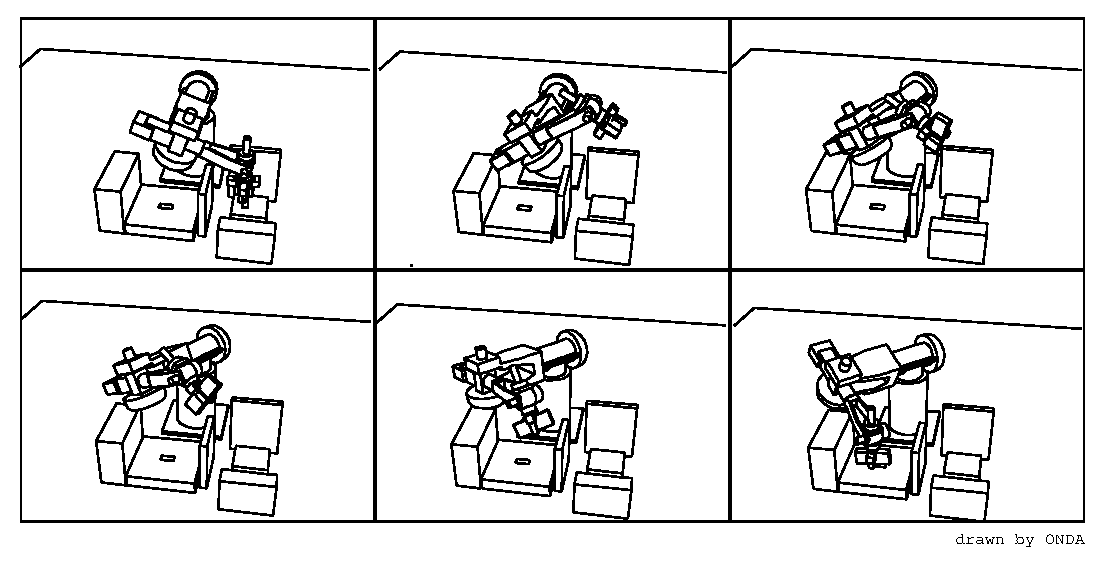
\includegraphics[width=150mm]{fig/eta3colavo.ps}
% \epsfile{file=fig/eta3colavo.ps,width=150mm}
%\mbox{
%\epsfxsize=15cm
%\epsfbox{fig/eta3colavo.ps}
%}
\caption{Animation of Collision Avoidance Path Planning}
\end{figure}

%\bibliography{/usr/users/matsui/biblio/lang,/usr/users/matsui/biblio/hirukawa}

\newpage


\section{Data Types}
\markright{\arabic{section}. Data Types}
Like other Lisps, it is data objects that are typed, not variables.
Any variable can have any object as its value.
Although it is possible to
declare the type of object which is bound to a variable, but usually
it is only advisory information to the compiler to generate faster code.
Numbers are represented as immediate values in pointers and all the others
are represented by objects referenced by pointers.

In the implementation of Sun4, a pointer or a number is represented by
a long word as depicted in fig.\ref{Pointer}.
Two bits at LSB of a pointer are used as tag bits to discriminate
between a pointer, an integer, and a float.
Since a pointer's tags are all zero and it can use all 32 bits for
addressing an object, EusLisp can utilize up to 4GB of process
address space.

\begin{figure}[hb]
\begin{center}
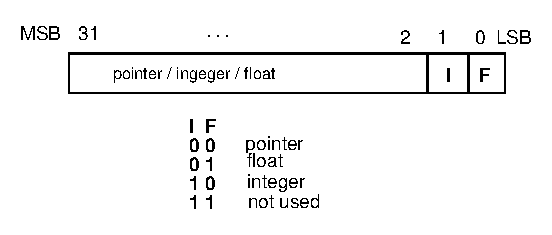
\includegraphics[width=10cm]{fig/pointer.ps}
% \epsfile{file=fig/pointer.ps}
%\mbox{
%\epsfxsize=10cm
%\epsfbox{fig/pointer.ps}
%}
\end{center}
\caption{\label{Pointer}Pointer and Immediate Value}
\end{figure}

\subsection{Numbers}

There are two kinds of numbers,
integer and float (floating-point number), both are represented
with 29 bits value and 1 bit sign.
Thus, integers range from -536,870,912 to 536,870,911.
Floats can represent plus/minus from 4.8E-38 to 3.8E38 with the
approximate accuracy of 6 digits in decimal, i.e.,
floating-point epsilon is approximately 1/1,000,000.

Numbers are always represented by immediate data, and not by objects.
This is the only exception of EusLisp's object orientation.
However, since numbers never waste heap memory, number crunching applications
run efficiently without causing garbage collection.

EusLisp does not have the character type,
and characters are represented by integers.
In order to write a program independent of character code sets,
%\#$\backslash$
\verb+#\+ reader dispatch macro is used.
However, when the character is read,
it is converted to numerical representation, and the printer does not
know how to reconvert it to
%\#$\backslash$
\verb+#\+ notation.

A number has two tag bits in a long word {Figure \ref{Pointer}},
which must be stripped off by shifting or masking 
when used in arithmetic computation.
Note that an integer should ignore two MSB bits by arithmetic shifting,
while a float should ignore two LSB bits by masking.
Byte swap is also necessary for an architecture like VAX which does not use
the rightmost byte as the least-significant mantissa byte.


\subsection{Objects}
Every data  other than number is represented by an object which is allocated
in heap. 
Each memory cell of an object has the object header and fixed number of 
slots for object variables.
Since vectors may consist of arbitrary number of elements,
they have 'size' slot immediately after the header.
Fig. \ref{ObjectFig} depicts the structures of object and vector, and their
header word.
Only the words indicated as {\em slot} and {\em element}
are accessible from users.

\begin{figure}[hbt]
\begin{center}
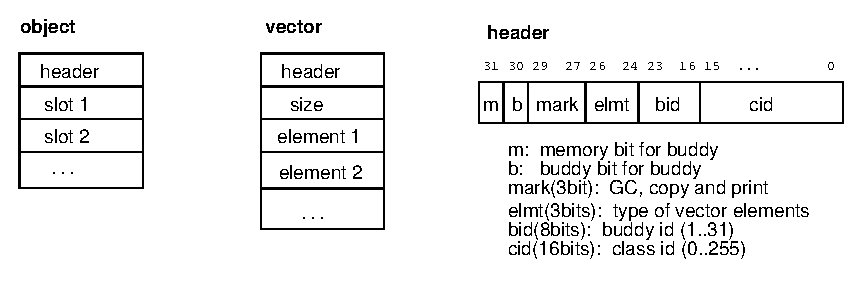
\includegraphics{fig/object.ps}
%\epsfile{file=fig/object.ps}
\end{center}
\caption{\label{ObjectFig}Structures of object, vector, and object header}
\end{figure}

A header is composed of six fields.
Two MSB bits, {\em m} and {\em b},
are used to indicate the side of the neighbor cell
in Fibonacci-buddy memory management.
There are three mark bits in the {\em mark} field, each of which
is used by the garbage collector to identify accessible cells,
by the printer to recognize circular objects in printing in {\tt \#n=} and
{\tt \#n\#} notations,
and by {\bf copy-object} to copy shared objects.
The {\em elmt} field discriminates one of seven possible data types
of vector elements, {\em pointer, bit, character, byte, integer, float}
and {\em foreign-string}.
Although {\em elmt} can be available in the class, 
it is provided in the header to make the memory manager independent of
the structure of a class and to make the element accessing faster.
The {\em bid} field represents the physical size of a memory cell.
31 different sizes up to 16 MB are represented by the five bits in this field.
%with relatively finer resolution than the binary buddy method.
The lower short word (16 bits) is used for the class id.
This is used to retrieve the class of an object via the system's class table.
This class id can be regarded as the type tag of traditional Lisps.
Currently only the lower 8 bits of the cid are used and the upper 8 bits
are ignored.
Therefore, the maximum number of classes is limited to 256, though
this limit can be raised up to 65536 by reconfiguring the EusLisp to allocate
more memory to the system's class table.

\subsection{Class Hierarchy}

The data structure of objects are defined by classes,
and their behaviors are defined by methods in the classes.
In EusLisp, a few dozens of classes have already been 
defined in tree structured
hierarchy as depicted in fig. \ref{ClassHierarchy}.
You can browse the real inheritance structure by the 
{\bf class-hierarchy} function.
The class 'object' at the leftmost is the ultimate super-class of
all the classes in EusLisp.
User-defined classes can inherit any of these built-in classes.

\begin{figure}
\small
\begin{verbatim}
object
     cons
          queue
     propertied-object
          symbol   -----  foreign-pod
          package
          stream
               file-stream
               broadcast-stream
          io-stream ---- socket-stream
          metaclass
               vectorclass
                    cstructclass
          read-table
          array
          thread
          barrier-synch
          synch-memory-port
          coordinates
               cascaded-coords
                    body
                    sphere
                    viewing
                         projection
                              viewing2d
                              parallel-viewing
                              perspective-viewing
                    coordinates-axes
               viewport
          line --- edge --- winged-edge
          plane
               polygon
                    face
                    hole
               semi-space
          viewer
          viewsurface  ----- tektro-viewsurface
     compiled-code
          foreign-code
          closure
          load-module
     label-reference
     vector
          float-vector
          integer-vector
          string
               socket-address
               cstruct
          bit-vector
          foreign-string
     socket-port
     pathname
     hash-table
     surrounding-box
     stereo-viewing
\end{verbatim}
\normalsize
\caption{\label{ClassHierarchy}Hierarchy of Predefined Classes}
\end{figure}

A class is defined the {\bf defclass} macro or by the {\bf defstruct} macro.

\ptext{
(defclass class-name \&key \= :super \hspace{15mm} \= class \\
 \> :slots \> () \\
 \> :metaclass \> metaclass \\
 \> :element-type \> t \\
 \> :size  -1\\ ) \\
(defstruct struct-name slots...) \\
(defstruct (struct-name [struct-options ...]) \\
\hspace{25mm}        (slot-name1 [slot-option...]) \\
\hspace{25mm}        (slot-name2 [slot-option...]) \\
\hspace{25mm}         ...) \\}

Methods are defined by the {\bf defmethod} special form.
{\bf Defmethod} can appear any times for a particular class.

\ptext{
(defmethod class-name  \\
 (:method-name1 (parameter...) . body1) \\
 (:method-name2 (parameter...) . body2) \\
 ...)
}

Field definitions for most of built-in classes are found in
{\tt *eusdir*/c/eus.h} header file.
{\tt (describe)} {\em class}) gives the description
of all the slots in {\em class}, namely, super class, slot names,
slot types, method list, and so on.
Definitions of built-in classes follow.
Note that the superclass of class {\bf object} is NIL
since it has no super class.

\ptext{
(defclass {\bf object} :super {\bf NIL} :slots ())
}

\ptext{
(defclass {\bf cons} :super {\bf object} :slots (car cdr))
}

\ptext{
(defclass {\bf propertied-object} :super {\bf object} \\
 \hspace{20mm} \=   :slots (plist)) \hspace{10mm} ;property list \\
}

\ptext{
(defclass {\bf symbol} :super {\bf propertied-object} \\
\hspace{20mm} :slots (\=value \hspace{15mm} \= ;specially bound value \\
 \>      vtype \>                ;const(0),var(1),special(2)  \\
 \>      function \>             ;global func def \\
 \>      pname               \>  ;print name string \\
 \>      homepkg)) \>            ;home package \\}

\ptext{
(defclass {\bf foreign-pod} :super {\bf symbol} \\
\hspace{20mm} :slots (\=podcode \hspace{15mm} \= ;entry code \\
 \>      paramtypes \>      ;type of arguments  \\
 \>      resulttype)) \\}


\ptext{
(defclass {\bf package} :super {\bf propertied-object} \\
\hspace{20mm} :slots (\= names \hspace{15mm} \= ;list of package name and nicknames\\
\>                   uses \>  ;spread use-package list \\
\>                   symvector \> ;hashed obvector \\
\>                   symcount \>  ;number of interned symbols \\
\>                   intsymvector \> ;hashed obvector of internal symbols \\
\>                   intsymcount \>  ;number of interned internal symbols \\
\>                   shadows \> ;shadowed symbols \\
\>                   used-by)) \>  ;packages using this package \\}

\ptext{
(defclass {\bf stream} :super {\bf propertied-object} \hspace{20mm} \\
\hspace{20mm} :slots (\= direction \hspace{3mm} \= ;:input or :output, nil if closed \\
  \>                   buffer  \>  ;buffer string \\
  \>                   count \> ;current character index \\
  \>                   tail)) \>  ;last character index \\
}

\ptext{
(defclass {\bf file-stream} :super {\bf stream} \\
\hspace{20mm} :slots (\= fd \hspace{10mm} \= ;file descriptor (integer)\\
 \>                    fname))\> ;file name str; qid for msgq \\
}

\ptext{
(defclass {\bf broadcast-stream} :super {\bf stream}\\
\hspace{20mm} :slots (destinations)) \hspace{10mm} ;streams to which output is delivered}

\ptext{
(defclass {\bf io-stream} \= :super {\bf propertied-object}\\
\>        :slots (instream outstream))}

\ptext{
(defclass {\bf socket-stream} \= :super {\bf io-stream}\\
\>        :slots (address)) \hspace{20mm} ; socket address}

\ptext{
(defclass {\bf read-table}  :super {\bf propertied-object} \\
\hspace{20mm}      :slots (\= syntax \hspace{10mm} \= ; byte vector representing character types \\
\>\> ; 0:illegal, 1:white, 2:comment, 3:macro\\
\>\> ; 4:constituent, 5:single\_escape\\
\>\> ; 6:multi\_escape, 7:term\_macro, 8:nonterm\_macro \\
\> macro \> ;character macro expansion function\\
\> dispatch-macro)) \\}

\ptext{
(defclass {\bf array} :super {\bf propertied-object} \\
\hspace{20mm} :slots (\= entity \hspace{12mm}\= ;simple vector storing array entity \\
 \>           rank  \> ;number of dimensions: 0-7 \\
 \>           fillpointer \>    ;pointer to push next element \\
 \>           offset      \>    ;offset for displaced array \\
 \>           dim0,dim1,dim2,dim3,dim4,dim5,dim6))  ;dimensions \\}

\ptext{
(defclass {\bf metaclass} :super {\bf propertied-object} \\
\hspace{20mm}   :slots   (\= name  \hspace{8mm} \= ;class name symbol \\
 \>           super   \>   ;super class \\
 \>           cix  \>      ;class id \\
 \>           vars  \>     ;var name vector including inherited vars \\
 \>           types  \>    ;type vector of object variables \\
 \>           forwards \>  ;components to which messages are forwarded \\
 \>           methods))  \>  ;method list \\ }

\ptext{
(defclass {\bf vectorclass} :super {\bf metaclass}  \\
\hspace{20mm} :slots (\= element-type  \hspace{4mm} \= ;vector element type 0-7\\
 \>                 size)) \>  ;vector size; 0 if unspecified \\ }

\ptext{
(defclass {\bf cstructclass} :super {\bf vectorclass}  \\
\hspace{20mm} :slots (\= slotlist))  \hspace{4mm} \= ;cstruct slot descriptors\\
}

\ptext{
(defclass {\bf vector} :super {\bf object} :slots (size))}

\ptext{
(defclass {\bf float-vector} :super {\bf vector} :element-type :float)}

\ptext{
(defclass {\bf string} :super {\bf vector} :element-type :char)}

\ptext{
(defclass {\bf hash-table} :super {\bf propertied-object} \\
\hspace{20mm}  :slots   (\= lisp::key \hspace{20mm}\= ;hashed key vector\\
\> value \> ; value vector\\
\> size \> ; the size of the hash table\\
\> count \> ; number of elements entered in the table\\
\> lisp::hash-function \> \\
\> lisp::test-function \\
\> lisp::rehash-size \\
\> lisp::empty  lisp::deleted \>) \\
}

\ptext{
(defclass {\bf queue} :super {\bf cons})}

\ptext{
(defclass {\bf pathname} :super {\bf propertied-object} \\
\hspace{20mm}  :slots   (\= lisp::host device \hspace{20mm}\= ; not used\\
\> directory \> ; list of directories\\
\> name \> ; file name before the last "."\\
\> type \> ; type field after the last "."\\
\> lisp::version) \> ; not used \\
}

\ptext{
(defclass {\bf label-reference} \hspace{8mm}  ;for reading \#n=, \#n\# objects \\
\hspace{20mm} \= :super {\bf object} \\
\>   :slots (label value unsolved next)) \\}

\ptext{
(defclass {\bf compiled-code} :super {\bf object} \\
\hspace{20mm}  :slots   (\= codevector \\
 \>          quotevector \\
 \>          type \hspace{15mm} \=    ;0=func, 1=macro, 2=special \\
 \>          entry))  \>  ;entry offset }

\ptext{
(defclass {\bf closure} \= :super {\bf compiled-code} \\
\>              :slots (env1 env2));environment}

\ptext{
(defclass {\bf foreign-code}  :super {\bf compiled-code}  \\
\hspace{20mm}  :slots   (\= paramtypes  \hspace{10mm} \=  ;list of parameter types\\
 \>              resulttype)) \> ;function result type}

\ptext{
(defclass {\bf load-module}  :super {\bf compiled-code}  \\
 \hspace{15mm}  :slots  (\= symbol-table \hspace{3mm} \= ;hashtable of symbols defined \\
 \>         object-file \> ;name of the object file loaded, needed for unloading \\
 \>         handle \> ;file handle returned by ''dlopen''}

\subsection{Type Specifier}
Though EusLisp does not have the {\bfx deftype} special form,
type names are used in declarations and functions requesting
to specify the type of results or contents,
as in {\bf coerce, map, concatenate, make-array}, etc.
Usually, class names can be used as type specifiers, as in
{\tt (concatenate cons "ab" "cd") = (97 98 99 100)},
where Common Lisp uses {\tt (quote list)} instead of {\tt cons}.

As EusLisp does not have classes to represent numbers,
types for numbers need to be given by keywords.
{\bfx :integer}, {\bfx integer}, {\bfx :int}, {\bfx fixnum},
or {\bfx :fixnum} is used to represent the integer type,
{\bfx :float} or {\bfx float}, the floating point number type.
As the {\emx element-type} argument of {\bfx make-array},
{\bfx :character}, {\bfx character}, {\bfx :byte}, and {\bfx byte}
are recognized to make strings.
Low level functions such as {\bfx defcstruct}, {\bfx sys:peek},
and {\bfx sys:poke}, also recognize
{\bfx :character}, {\bfx character}, {\bfx :byte}, or {\bfx byte}
for the byte access, and {\bfx :short} or {\bfx short} for short word access.
In any cases, keywords are preferable to lisp package symbols with the
same pname.

\newpage

\section{Forms and Evaluation}
\markright{\arabic{section}. Forms and Evaluation}
\subsection{Atoms}

A data object other than a cons is always an atom, no matter what complex
structure it may have.
Note that NIL, which is sometimes noted as () to represent an empty
list, is also an atom.
Every atom except a symbol is always evaluated to itself,
although quoting is required in some other Common Lisp implementations.

\subsection{Scoping}

Every symbol may have associated value.
A symbol is evaluated to its value determined in the current binding context.
There are two kinds of variable bindings;
the lexical or static binding and the special or dynamic binding.
Lexically bound variables are introduced by {\bf lambda} form or
{\bf let} and {\bf let*} special forms
unless they are declared special.
Lexical binding can be nested and the only one binding which is introduced
innermost level is visible, hiding outer lexical bindings and the special 
binding.
Special variables are used in two ways:
one is for global variables, and the other is for dynamically scoped
local variables which are visible even at the outside of
the lexical scope as long as the binding is in effect.
In the latter case, special variables are needed to be declared special.
The declaration is recognized not only by the compiler, but also by
the interpreter.
According to the Common Lisp's terms, special variables are said to have
indefinite scope and dynamic extent.
%\footnote{In Maclisp, all the variables are taken to be special by the
%interpreter, and lexical by the compiler if not declared special.
%In Etalisp, all variables are special and no declaration is recognized.}

Even if there exists a lexical variable in a certain scope,
the same variable name can be redeclared to be special in inner scope.
Function {\bf symbol-value} can be used to retrieve  the special values
regardless to the lexical scopes.
Note that {\bf set} function works only for special variable, i.e.
it cannot be used to change the value of lambda or let variables
unless they are declared special.

\begin{verbatim}
(let ((x 1))
   (declare (special x))
   (let* ((x (+ x x)) (y x))
      (let* ((y (+ y y)) (z (+ x x)))
         (declare (special x))
         (format t "x=~S y=~s z=~s~%" x y z) ) ) )
--> x=1 y=4 z=2
\end{verbatim}

A symbol can be declared to be a constant by {\bf defconstant} macro.
Once declared, an attempt to change the value signals an error thereafter.
Moreover, such a constant symbol is inhibited to be used as
the name of a variable even for a local variable.
NIL and T are examples of such constants.
Symbols in the keyword package are always declared to be constants
when they are created.
In contrast, {\bf defvar} and {\bf defparameter} macro declare
symbols to be special variables.
{\bf defvar} initializes the value only if the symbol is unbound,
and does nothing when it already has a value assigned,
while {\bf defparameter} always resets the value.

When a symbol is referenced and there is no lexical binding for the symbol,
its special value is retrieved.
However, if no value has been assigned to its special value yet,
unbound variable error is signaled.

\subsection{Generalized Variables}
Generally, any values or attributes are represented in slots of objects
(or in stack frames).
To retrieve and alter the value of a slot,
two primitive operations, {\em access} and {\em update}, must be provided.
Instead of defining two distinct primitives for every slot of objects,
EusLisp, like Common Lisp, provides uniform update operations
based on the generalized variable concept.
In this concept, a common form is recognized  either as a value access form
or as a slot location specifier.
Thus, you only need to remember accessing form for each slot and
update is achieved by {\bf setf} macro used in conjunction with the access form.
For example, {\tt (car x)} can be used to replace the value
in the car slot of {\tt x} when used with {\bf setf} as in {\tt (setf (car 
'(a b) 'c)},
as well as to take the car value out of the list.

This method is also applicable to all the user defined objects.
When a class or a structure is defined, the access and update forms
for each slot are automatically defined.
Each of those forms is defined as a macro whose name is the concatenation of
the class name and slot name.
For example, car of a cons can be addressed by {\tt (cons-car '(a b c))}.

\begin{verbatim}
(defclass person :super object :slots (name age))
(defclass programmer :super person :slots (language machine))
(setq x (instantiate programmer))
(setf (programmer-name x) "MATSUI"
      (person-age x) 30)
(incf (programmer-age x))
(programmer-age x)   --> 31
(setf (programmer-language x) 'EUSLISP
      (programmer-machine x) 'SUN4)
\end{verbatim}

Array elements can be accessed in the same manner.

\begin{verbatim}
(setq a (make-array '(3 3) :element-type :float))
(setf (aref a 0 0) 1.0 (aref a 1 1) 1.0 (aref a 2 2) 1.0)
a --> #2f((1.0 0.0 0.0) (0.0 1.0 0.0) (0.0 0.0 1.0))

(setq b (instantiate bit-vector 10))  --> #*0000000000
(setf (bit b 5) 1)
b --> #*0000010000
\end{verbatim}

In order to define special setf methods for particular objects,
{\bf defsetf} macro is provided.

\begin{verbatim}
(defsetf symbol-value set)
(defsetf get (sym prop) (val) `(putprop ,sym ,val ,prop))
\end{verbatim}

\subsection{Special Forms}

\begin{table}
\begin{center}
{\large
\begin{tabular}{|l l l|} \hline 
and & flet & quote \\
block & function & return-from\\
catch & go & setq \\
cond & if & tagbody \\
declare & labels & the \\
defmacro & let & throw \\
defmethod & let* & unwind-protect \\
defun & progn & while \\
eval-when & or & \\
\hline
\end{tabular} }
\end{center}
\caption{\label{SpecialForms}EusLisp's special forms}
\end{table}

All the special forms are listed in Table \ref{SpecialForms}.
{\bf macrolet, compiler-let,} and {\bf progv} have not been implemented.
Special forms are essential language constructs for the management of
evaluation contexts and control flows.
The interpreter and compiler have special knowledge to
process each of these constructs properly, while the application
method is uniform for all functions.
Users cannot add their own special form definition.

\subsection{Macros}

Macro is a convenient method to expand language constructs.
When a macro is called, arguments are passed to the macro body,
which is a macro expansion function, without being evaluated.
Then, the macro expansion function expands the arguments,
and returns the new form.
The resulted form is then evaluated again outside the macro.
It is an error to apply a macro or special form to a list of arguments.
{\bf Macroexpand} function can be used for the explicit macro expansion.

Though macro runs slowly when interpreted,
it speeds up compiled code execution,
because macro expansion is taken at compile-time only once
and no overhead is left to run-time.
Note that explicit call to eval or apply in the macro function may
produce different results between interpreted execution
and the compiled execution.

\subsection{Functions}

A function is expressed by a lambda form which is merely a list
whose first element is {\bf lambda}.
If a lambda form is defined for a symbol using {\bf defun}, it can be referred
as a global function name.
Lambda form takes following syntax.

\ptext{
(lambda (\= \{var\}* \\
\>  [\&optional \{var $|$ (var [initform])\}*] \\
\>  [\&rest form] \\
\>  [\&key \= \{var $|$ (var [initform]) $|$ ((keyword var) [initform])\}* \\
\> \> [\&allow-other-keys]] \\
\>  [\&aux \{var $|$ (var [initform])\}*]) \\
 \hspace{10mm} \{declaration\}* \\
 \hspace{10mm} \{form\}*) \\
}

There is no function type such as EXPR, LEXPR, FEXPR, etc.:
arguments to a function are always evaluated before its application,
and the number of acceptable arguments is determined by lambda-list.
Lambda-list specifies the sequence of parameters to the lambda form.
Each of {\bf \&optional, \&rest, \&key } and {\bf \&aux} has special
meaning in lambda-lists, and these symbols cannot be used as variable
names.
Supplied-p variables for \&optional or \&key parameters are not supported.

Since a lambda form is indistinguishable from normal list data,
{\bf function} special form must be used to inform the interpreter and
compiler the form is intended to be a function.
\footnote{In CLtL-2 a quoted lambda form is no longer a function.
Application of such a form is an error.}
{\bf Function} is also important to freeze the environment onto the function,
so that all the lexical variables can be accessible in the function
even the function is passed to another function of different lexical scope.
The following program does not work either interpretedly nor after compiled,
since {\tt sum} from the {\tt let} is invisible  inside lambda form.

\begin{verbatim}
(let ((x '(1 2 3)) (sum 0))
  (mapc '(lambda (x) (setq sum (+ sum x))) x))
\end{verbatim}

To get the expected result, it should be written as follows:
\begin{verbatim}
(let ((x '(1 2 3)) (sum 0))
   (mapc #'(lambda (x) (setq sum (+ sum x))) x ))
\end{verbatim}

\#' is the abbreviated notation of {\bf function},
i.e. {\tt \#'(lambda (x) x)} is equivalent to
{\tt (function (lambda (x) x))}.
Here is another example of what is called a funarg problem:

\begin{verbatim}
(defun mapvector (f v)
    (do ((i 0 (1+ i)))
       ((>= i (length v)))
       (funcall f (aref v i))))
(defun vector-sum (v)
    (let ((i 0))
       (mapvector #'(lambda (x) (setq i (+ i x))) v)
       i))
(vector-sum #(1 2 3 4)) --> 10 
\end{verbatim}

EusLisp's closure cannot have indefinite extent:
i.e. a closure can only survive as long as its outer extent is in effect.
This means that a closure cannot be used for programming of ``generators".
The following program does not work.

\begin{verbatim}
(proclaim '(special gen))
(let ((index 0))
   (setq gen #'(lambda () (setq index (1+ index)))))
(funcall gen)
\end{verbatim}

However, the same purpose is accomplished by object oriented programming,
because an object can hold its own static variables:
\begin{verbatim}
(defclass generator object (index))
(defmethod generator
 (:next () (setq index (1+ index)))
 (:init (&optional (start 0)) (setq index start) self))
(defvar gen (instance generator :init 0))
(send gen :next)
\end{verbatim}
\newpage

\section{Control Structures}
\markright{\arabic{section}. Control Structures}
\subsection{Conditionals}

Although {\bf and, or} and {\bf cond} are advised to be macros by Common Lisp,
they are implemented as special forms in EusLisp to improve
the interpreting performance.

\begin{refdesc}
\specialdesc{and}{\{form\}*}{
{\em Form}s are evaluated from left to right until NIL appears.
If all forms are evaluated to non-NIL, the last value is returned.}

\specialdesc{or}{\{form\}*}{
{\em Form}s are evaluated from left to right until non-NIL appears,
and the value is returned. If all forms are evaluated to NIL, 
NIL is returned.}

\specialdesc{if}{test then [else]}{
{\bf if} can only have single {\it then} and {\it else} forms.
To allow multiple {\em then} or {\em else} forms,
they must be grouped by {\bf progn}.}

\macrodesc{when}{test forms}{
Unlike {\bf if},
{\bf when} and {\bf unless} allow you to write multiple {\em forms}
which are executed when {\em test} holds ({\bf when}) or
does not {\em unless}.
On the other hand, these macros
cannot have the {\em else} forms.}

\macrodesc{unless}{test forms}{
is equivalent to {\tt(when (not {\em test}) . {\em forms})}.}

\specialdesc{cond}{{(test \{form\}*)}*}{
Arbitrary number of  cond-clauses can follow {\bf cond}.
In each clause, the first form, that is {\em test}, is evaluated.
If it is non-nil, the rest of the forms in that clause are evaluated sequentially,
and the last value is returned. 
If no forms are given after the {\em test}, the value of the {\em test} is returned.
When the {\em test} fails, next clause is tried until a {\em test} which is evaluated
to non-nil is found or all clauses are exhausted.
In the latter case, {\bf cond} returns NIL.}

\macrodesc{case}{key \{(\{label $|$ (\{lab\}*) \{form\}*)\}*}{
For the clause whose {\em label} matches with {\em key},
{\em form}s are evaluated and the last value is returned.
Equality between {\em key} and {\em label} is tested with {\bf eq}
or {\bf memq}, not with {\bf equal}.}

\end{refdesc}

\subsection{Sequencing and Lets}

\begin{refdesc}
\funcdesc{prog1}{form1 \&rest forms}{
{\em form1} and {\em forms} are evaluated sequentially, 
and the value returned by {\em form1} is returned as the value of {\bf prog1}.}

\specialdesc{progn}{\{form\}*}{
{\em Form}s are evaluated sequentially, and the value of the rightmost form
is returned.
{\bf Progn} is a special form because it has a special meaning when it
appeared at top level in a file.
When such a form is compiled, all inner forms are regarded as they appear
at top level.
This is useful for a macro which expands to a series of
{\bf defun}s or {\bf defmethod}s, which must appear at top level.}

\macrodesc{setf}{\{access-form value\}*}{
assigns {\em value} to a generalized-variable {\em access-form}.}

\specialdesc{let}{(\{var $|$ (var [value])\}*) \{declare\}* \{form\}*}{
introduces local variables.
All {\em value}s are evaluated and assigned to {\em var}s in parallel, i.e.,
{\tt (let ((a 1)) (let ((a (1+ a)) (b a)) (list a b)))} produces
(2 1).}

\specialdesc{let*}{(\{var $|$ (var [value])\}*) \{declare\}* \{form\}*}{
introduces local variables.
All {\em value}s are evaluated sequentially, and assigned to {\em var}s
i.e.,
{\tt (let ((a 1)) (let* ((a (1+ a)) (b a)) (list a b)))} produces
(2 2).}
\end{refdesc}

\subsection{Local Functions}
\begin{refdesc}
\specialdesc{flet}{ (\{(fname lambda-list . body)\}*) \{form\}*}{
defines local functions.}

\specialdesc{labels}{ (\{(fname lambda-list . body)\}*) \{form\}*}{
defines locally scoped functions. 
The difference between {\em flet} and {\em labels} is,
the local functions defined by {\em flet} cannot reference
each other or recursively, whereas {\em labels} allows such mutual references.}
\end{refdesc}

\subsection{Blocks and Exits}
\begin{refdesc}
\specialdesc{block}{tag \{form\}*}{
makes a lexical block from which you can exit by {\bf return-from}.
{\em Tag} is lexically scoped and is not evaluated.}

\specialdesc{return-from}{tag value}{
exits the block labeled by {\em tag}.
{\bf return-from} can be used to exit from a function or a method which
automatically establishes block labeled by its function or method name
surrounding the entire body.}

\macrodesc{return}{value}{
{\tt  (return x)} is equivalent to {\tt (return-from nil x)}. This is
convenient to use in conjunction with {\bf loop, while, do, dolist,}
and {\bf dotimes} which implicitly establish blocks labeled NIL.}

\specialdesc{catch}{ tag \{form\}*}{
establishes a dynamic block from which you can exit and return a value
by {\bf throw}. {\em Tag} is evaluated.
The list of all visible catch tags can be obtained by {\tt
sys:list-all-catchers}.}

\specialdesc{throw}{tag value}{
exits and returns {\em value} from a catch block.
{\em tag} and {\em value} are evaluated.}

\specialdesc{unwind-protect}{protected-form \{cleanup-form\}*}{
After the evaluation of {\em protected-form} finishes,
{\em cleanup-form} is evaluated.
You may make a block or a catch block outside the {\tt unwind-protect}.
Even {\bf return-from} or {\bf throw} is executed in {\em protected-form}
to escape from such blocks, {\em cleanup-form} is assured to be evaluated.
Also, if you had an error while executing {\em protected-form},
{\em cleanup-form} would always be executed by {\em reset}.}

\end{refdesc}

\subsection{Iteration}

\begin{refdesc}

\specialdesc{while}{test \{form\}*}{
While {\em test} is evaluated to non-nil,
{\em form}s are evaluated repeatedly.
{\bf While} special form automatically establishes a block by name of nil
around {\em form}s, and {\bf return} can be used to exit from the loop.}

\specialdesc{tagbody}{\{tag $|$ statement\}*}{
{\em tag}s are labels for {\bf go}.
You can use {\bf go} only in {\bf tagbody}.}

\specialdesc{go}{tag}{
transfers control to the form just after {\em tag}
which appears in a lexically scoped {\bf tagbody}.
{\bf Go} to the tag in a different {\bf tagbody}
across the lexical scope is inhibited.}

\macrodesc{prog}{(\{var $|$ (var [init])\}*) \{tag $|$ statement\}*}{
{\bf prog} is a macro, which expands as follows:
\ptext{
(block nil 
    (let {\em var}
	(tagbody
		{\em tag $|$ statement})))}
}

\macrodesc{do}{(\{(var init [next])\}*) (endtest [result])\{declare\} \{form\}
*}
{{\em var}s are local variables.
To each {\em var}, {\em init} is evaluated in parallel and assigned.
Next, {\em endtest} is evaluated and if it is true, {\bf do} returns
{\em result} (defaulted to NIL).
If {\em endtest} returns NIL, each {\em form} is evaluated sequentially.
After the evaluation of forms, {\em next} is evaluated and the value is
reassigned to each {\em var}, and the next iteration starts.}

\macrodesc{do*}{(\{var init [next]\}*) (endtest [result])\{declare\} \{form\}*}
{{\bf do*} is same as {\bf do} except that the evaluation of {\em init}
and {\em next}, and their assignment to {\em var} occur sequentially.}

\macrodesc{dotimes}{(var count [result]) \{forms\}*}{
evaluates {\em forms} {\em count} times.
{\em count} is evaluated only once.
In each evaluation, {\em var} increments from integer zero to
{\em count} minus one.}

\macrodesc{dolist}{(var list [result]) \{forms\}*}{
Each element of {\em list} is  sequentially bound to {\em var},
and {\em forms} are evaluated for each binding.
{\bf Dolist} runs faster than other iteration constructs
such as {\bf mapcar} and recursive functions,
since {\bf dolist} does not have to create a function closure or to apply it,
and no new parameter binding is needed.}

\macrodesc{until}{condition \{forms\}*}{
evaluates forms until {\em condition} holds.}

\macrodesc{loop}{\{forms\}*}{
evaluates {\em forms} forever.
To terminate execution, {\bf return-from, throw} or {\bf go} needed to be
evaluated in {\em forms}.}

\subsection{Predicates}

{\bf Typep} and {\bf subtypep} of Common Lisp are not provided, and should be
simulated by {\bf subclassp} and {\bf derivedp}.

\begin{refdesc}

\funcdesc{eq}{obj1 obj2}{returns T,
if {\em obj1} and {\em obj2} are pointers to the same object,
or the same numbers.
Examples: {\tt (eq 'a 'a)} is T, {\tt (eq 1 1)} is T,
{\tt (eq 1. 1.0)} is nil, {\tt (eq "a" "a")} is nil.}
\funcdesc{eql}{obj1 obj2}{
{\bf Eq} and {\bf eql} are identical since all the numbers in EusLisp are represented as
immediate values.}
\funcdesc{equal}{obj1 obj2}{
Checks the equality of any structured objects, such as strings, vectors or
matrices, as long as they do not have recursive references.
If there is recursive reference in {\em obj1} or {\em obj2},
{\bf equal} loops infinitely.}
\funcdesc{superequal}{obj1 obj2}{
Slow but robust {\bf equal}, since {\bf superequal} checks circular reference.}

\funcdesc{null}{object}{T if {\em object} is nil.
Equivalent to (eq {\em object} nil).}
\funcdesc{not}{object}{
{\bf not} is identical to {\bf null}.}
\funcdesc{atom}{object}{
returns NIL only if object is a cons.
{\tt (atom nil) = (atom '()) = T)}.
Note that {\bf atom} returns T for vectors, strings, read-table, hash-table, 
etc., no matter what complex objects they are.}
\funcdesc{every}{pred \&rest args}{
returns T if all {\em args} return T for {\em pred}.
{\bf Every} is used to test whether {\em pred} holds for every {\em args}.}
\funcdesc{some}{pred \&rest args}{
returns T if at least one of {\em args} return T for {\em pred}.
{\bf Some} is used to test whether {\em pred} holds for any of {\em args}.}
\end{refdesc}
\funcdesc{functionp}{object}{
T if {\em object} is a function object that can be given to
{\bf apply} and {\bf funcall}.
Note that macros cannot be {\em apply}'ed or {\em funcall}'ed.
{\bf Functionp} returns T, if {\em object} is
either a compiled-code with type=0, a symbol that has function definition,
a lambda-form, or a lambda-closure.
Examples: (functionp 'car) = T, (functionp 'do) = NIL} 
\funcdesc{compiled-function-p}{object}{
T if {\em object} is an instance of compiled-code.
In order to know the compiled-code is a function or a macro,
send {\tt :type} message to the object, and {\tt function} or {\tt macro}
is returned.}

\end{refdesc}

\newpage

\section{Object Oriented Programming}
\markright{\arabic{section}. Object-Oriented Programming}

The structures and behaviors of objects are described in
classes, which are defined by
{\bf defclass} macro and {\bf defmethod} special form.
{\bf defclass} defines the name of the class, its super class, and
slot variable names, optionally with their types and message forwarding.
{\bf defmethod} defines methods which will invoked when
corresponding messages are sent.
Class definition is assigned to the symbol's special value.
You may think of {\bf class} as 
the counter part of Common Lisp's {\bf structure}.
Slot accessing functions and {\bf setf} methods are automatically defined
for each slot by {\bf defclass}.

Most classes are instantiated from the built-in class {\bf metaclass}.
Class {\bf vector-class}, which is a subclass of {\bf metaclass},
is a metaclass for vectors.
If you need to use class-variables and class-methods,
you may make your own metaclass by subclassing {\bf metaclass},
and the metaclass name should be given to {\bf defclass} with
{\tt :metaclass} keyword.

Vectors are different from other record-like objects
because an instance of the vector can have arbitrary number of elements,
while record-like objects have fixed number of slots.
EusLisp's object is either a record-like object or a vector, not both
at the same time.

Vectors whose elements are typed or the number of elements are
unchangeable can also be defined by {\bf defclass}.
In the following example,
class {\tt intvec5} which has five integer elements is defined.
Automatic type check and conversion are performed when the elements are
accessed by the interpreter.
When compiled with proper declaration, faster accessing code is produced.

\begin{verbatim}
(defclass intvec5 :super vector :element-type :integer :size 5)
(setq x (instantiate intvec5))  --> #i(0 0 0 0 0)
\end{verbatim}

When a message is sent to an object, 
the corresponding method is searched for, first in its class,
and next in its superclasses toward {\bf object},
until all superclasses are exhausted.
If the method is undefined, forward list is searched.
This forwarding mechanism is introduced to simulate multiple inheritance.
If the search fails again, a method named {\tt :nomethod} is searched,
and the method is invoked with a list of all the arguments.
In the following example, the messages {\tt :telephone} and {\tt :mail} are
sent to {\tt secretary} slot object which is typed {\tt person},
and {\tt :go-home} message is sent to {\tt chauffeur} slot.

\begin{verbatim}
(defclass president :super object
                    :slots ((name :type string)
                            (age  :type :integer)
                            (secretary  :type person
                                        :forward (:telephone :mail))
                            (chauffeur  :forward (:go-home))))
\end{verbatim}

In a method, two more local variables,
{\bf class} and {\bf self}, become accessible.
You should not change either of these variables.
If you do that, the ones supplied by the system are hidden,
and {\bf send-super} and {\bf send self} are confused.


\subsection{Classes and Methods}

\begin{refdesc}

\longdescription{defclass}
{classname \&key \= :super object \` [macro] \\
\> :slots (\{var $|$ (var [:type type] [:forward selectors])\}*) \\
\> :metaclass metaclass \\
\> :element-type t \\
\> :size -1\\}
{creates or redefine a class.
When a class is redefined to have different superclass or slot variables,
old objects instantiated from the previous class definition will 
behave unexpectedly, since method definitions assume the new slots
disposition.}

\specialdesc{defmethod}{classname \{(selector lambda-list . body)\}*}{
defines one or more methods of {\em classname}. Each {\em selector}
must be a keyword symbol.}

\macdesc{defclassmethod}{classname \{(selector lambda-list . body)\}*}

\funcdesc{classp}{object}{T if {\em object} is a class object, that is,
an instance of class {\bf metaclass} or its subclasses.}

\funcdesc{subclassp}{class super}{
Checks {\em class} is a subclass of {\em super}.}

\funcdesc{vector-class-p}{x}{T if {\em x} is an instance of {\bf vector-class}.}

\funcdesc{delete-method}{class method-name}{
The method definition is removed from the specified class.}

\funcdesc{class-hierarchy}{class}{
prints inheritance hierarchy below {\em class}.}

\funcdesc{system:list-all-classes}{}{
lists up all the classes defined so far.}

\funcdesc{system:find-method}{object selector}{
tries to find a method specified by {\em selector} in the class of {\em object}
and in its superclass.
This is used to know whether {\em object} can respond to {\em selector}.}

\funcdesc{system:method-cache}{[flag]}{
Interrogates the hit ratio of the method cache,
and returns a list of two numbers, hit and miss.
If {\em flag} is NIL, method caching is disabled.
If non-nil flag is given, method cache is purged and caching is enabled.}

\end{refdesc}

\subsection{Message Sending}
\begin{refdesc}

\funcdesc{send}{object selector \{arg\}*}{
send a message consisting of {\em selector} and {\em arg} to {\em object}.
{\em object} can be anything but number.
{\em selector} must be evaluated to be a keyword.}

\funcdesc{send-message}{target search selector \{arg\}*}{
Low level primitive to implement {\bf send-super}.}

\macrodesc{send*}{object selector \&rest msg-list}{
{\bf send*} applies {\bf send-message} to a list of arguments.
The relation between {\bf send} and {\bf send*} is like the one
between {\bf funcall} and {\bf apply}, or {\bf list} and {\bf list*}.}

\funcdesc{send-all}{receivers selector \&rest mesg}{
sends the same message to all the receivers, and collects the result
in a list.}

\macrodesc{send-super}{selector \&rest msgs}{
sends {\em msgs} to self, but
begins method searching at the superclass of the class
where the method currently being executed is defined.
It is an error to {\em send-super} outside a method (i.e. in a function).}

\macrodesc{send-super*}{selector \&rest msg-list}{
{\bf send-super*} is apply version of send-super.}

\end{refdesc}

\subsection{Instance Management}

\begin{refdesc}

\funcdesc{instantiate}{class \&optional size}{
the lowest primitive to create a new object from a class.
If the class is a vector-class, {\em size} should be supplied.}

\macrodesc{instance}{class \&rest message}{
An instance is created, and the message is sent to it.}

\funcdesc{make-instance}{class \&rest var-val-pairs}{
creates an instance of {\em class} and sets its slot variables
according to {\em var-val-pairs}.
For example, {\tt (make-instance cons :car 1 :cdr 2)}
is equivalent to {\tt (cons 1 2)}.}

\funcdesc{copy-object}{object}{
{\bf copy-object} function is used to copy objects keeping the referencing
topologies even they have recursive references.
{\bf Copy-object} copies any objects accessible from {\em object}
except symbols and packages, which are untouched to keep the uniqueness
of symbols.
{\bf copy-object} traverses all the references in an object twice:
once to create new objects and to mark original objects that they have
already copied, and again to remove marks.
This two-step process makes copy-object work slower than copy-seq.
If what you wish to copy is definitely a sequence,
use of {\bf copy-seq} or {\bf copy-tree} is recommended.}

\funcdesc{become}{object class}{
changes the class of {\em object} to {\em class}.
The slot structure of both the old class and the new class must be
consistent. Usually, this can be safely used only for changing
class between binary vectors, for example from an integer-vector
to a bit-vector.}

\funcdesc{replace-object}{dest src}{
dest must be an instance of the subclass of src.}

\funcdesc{class}{object}{
returns the class object of {\em object}.
To get the name of the class, send :name message to the class object.}

\funcdesc{derivedp}{object class}{
{\bf derivedp} checks if an object is instantiated from {\em class}
or {\em class}'s subclasses.
{\bf subclassp} and {\bf derivedp} functions do not search in class hierarchy:
type check always finishes within a constant time.}

\funcdesc{slot}{object class (index $|$ slot-name)}{
Returns the named or indexed slot value.}

\funcdesc{setslot}{object class (index $|$ slot-name) value}{
{\bf Setslot} is a internal function and users should not use it.
Use, instead, combination of {\bf setf} and {\bf slot}.}

\end{refdesc}

\subsection{Basic Classes}

\begin{refdesc}
\classdesc{object}{}
{}
{Object is the most basic class that is located at the top of class hierarchy.
Since it defines no slot variables, it is no use to make an instance of
{\bf object}.}

\methoddesc{:prin1}{\&optional stream \&rest mesg}{
prints the object in the standard re-readable object format,
that is, the class name and the address, enclosed by angle brackets and
preceded by a pound sign.
Any subclasses of {\bf object} can use this method to print itself with
more comprehensive information  by using
{\bf send-super} macro specifying {\em mesg} string.
An object is re-readable if it begins with \#$<$,
followed by its class name, correct address, any lisp-readable information,
and \verb+>+.
Since every data object except numbers inherits {\bf object},
you can get print forms in this notation, even for symbols or strings.
Specifying this notation, you can catch data objects that you forgot
to {\bf setq} to a symbol, as long as there happened no garbage collection
after it is printed.}

\methoddesc{:slots}{}{
returns the list of variable-name and value pair of all the slots of the
object.
You can get the value of a specific slot by applying {\bf assoc} to this
list, although you cannot alter them.}

\classdesc{propertied-object}{object}
{plist}
{defines objects that have property list.
Unlike other Common Lisp, 
EusLisp allows any objects that inherit propertied-object to have property
lists, even if they are not symbols.}

\methoddesc{:plist}{\&optional plist}{
if {\em plist} is specified, it is set to the plist slot of this object.
Previous plist, if there had been one, is lost.
Legal plist should be of the form of
\verb+((indicator1 . value1) (indicator2 . value2) ...)+.
Each \verb+indicator+ can be any lisp form that are tested its equality
with the {\bf eq} function.
When a symbol is used for an indicator, use of keyword is recommended
to ensure the equality check will be performed interpacakge-widely.
{\bf :plist} returns the current plist.}

\methoddesc{:get}{indicator}{
returns the value associated with {\em indicator} in the property list.
\verb+(send x :get :y) == (cdr (assoc :y (send x :plist)))+.}

\methoddesc{:put}{indicator value}{
associates {\em value} to {\em indicator} in the plist.}

\methoddesc{:remprop}{indicator}{
removes {\em indicator} and value pair from the plist.
Further attempt to {\em :get} the value returns nil.}

\methoddesc{:name}{\&optional name}{
defines and retrieves the {\tt :name} property in the plist.
This property is used for printing.}

\methoddesc{:prin1}{\&optional stream \&rest mesg}{
prints the object in the re-readable form.
If the object has {\bf :name} property, it is printed after
the address of the object.}

\methoddesc{:slots}{}{
returns a list of variable and value pairs of this object.}

\methoddesc{:methods}{}{
returns a list of all method names defined for this object.
In other words, this object can accept method calls listed by :methods. }

\methoddesc{:get-val}{variable-name}{
returns the value of the slot designated by {\it variable-name}.
If the object does not have the variable-name slot, an error is reported.}

\methoddesc{:set-val}{variable-name value}{
sets {\it value} in the variable-name slot of this object.
If the object does not have the variable-name slot, an error is reported.}

\classdesc{metaclass}{propertied-object}
{name super cix vars types forwards methods}
{Metaclass defines classes. Classes that have own class variables
should be defined with {\bf metaclass} as their superclass.}
\methoddesc{:new}{}
{creates an instance of this class and returns it
after filling all the slots with NIL.}
\methoddesc{:super}{}{
returns the super class object of this class.
You cannot alter superclass once defclassed.}
\methoddesc{:methods}{}{
returns a list of all the methods defined in this class.
The list is composed of lists each of which describes the name of
the method, parameters, and body.}
\methoddesc{:method}{name}{
returns the method definition associated with {\em name}.
If not found, NIL is returned.}
\methoddesc{:method-names}{subname}{
returns a list of all the method names each of which contains
{\em subname} in its method name.
Methods are searched only in this class.}
\methoddesc{:all-methods}{}{
returns a list of all methods that are defined in this class and
its all the super classes.
In other words, an instance of this class can execute each of these
methods.}
\methoddesc{:all-method-names}{subname}{
returns a list of all the method names each of which matches with
{\em subname}.
The search is made from  this class up to {\bf object}.}
\methoddesc{:slots}{}{
returns the slot-name vector.}
\methoddesc{:name}{}{returns the name symbol of this class.}
\methoddesc{:cid}{}{
returns an integer that is assigned to every
instance of this class to identify its class.
This is an index to the system-internal class table, and is changed
when a new subclass is defined under this class.}
\methoddesc{:subclasses}{}{
returns a list of the direct subclass of this class.}
\methoddesc{:hierarchy}{}{
returns a list of all the subclasses defined under this class.
You can also call the {\bf class-hierarchy} function to get a comprehensive
listing of all the class hierarchy.}
\funcdesc{find-method}{object selector}{
searches for the method identified by {\em selector} in {\em object}'s
class and its super classes. This function is useful when object's
class is uncertain and you want to know whether the object can handle
the message without causing nomethod error.}
\end{refdesc}
\newpage

%\input{predicates}
\section{Arithmetic Functions}
\markright{\arabic{section}. Arithmetic}
\subsection{Arithmetic Constants}
\begin{refdesc}
\constdesc{most-positive-fixnum}{\#x1fffffff=536,870,911}
\constdesc{most-negative-fixnum}{-\#x20000000= -536,870,912}
\constdesc{short-float-epsilon}{
A floating point number on machines with IEEE floating-point format is
represented by 21 bit mantissa with 1 bit sign and 7 bit exponent with
1 bit sign.
Therefore, floating point epsilon is $2^{-21}= 4.768368 \times 10^{-7}$.}
\constdesc{single-float-epsilon}{same as {\bf short-float-epsilon}, $2^{-21}$.}
\constdesc{long-float-epsilon}{same as {\bf short-float-epsilon} since
there is no double or long float. $2^{-21}$.}
\constdesc{pi}{$\pi$, actually 3.14159203, not 3.14159265.}
\constdesc{2pi}{$2\times \pi$}
\constdesc{pi/2}{$\pi/2$}
\constdesc{-pi}{-3.14159203}
\constdesc{-2pi}{$-2\times \pi$}
\constdesc{-pi/2}{$\pi/2$}
\end{refdesc}

\subsection{Arithmetic Predicates}
\begin{refdesc}
\funcdesc{numberp}{object}{
T if {\em object} is number, namely integer or float.
Note that characters are also represented by numbers.}
\funcdesc{integerp}{object}{
T if {\em object} is an integer number.
A float can be converted to an integer by
{\bf round, trunc} and {\bf ceiling} functions.}
\funcdesc{floatp}{object}{T if {\em object} is a floating-point number.
An integer can be converted to a float by the {\bf float} function.}

\funcdesc{zerop}{number}{T if the number is integer zero or float 0.0.}
\funcdesc{plusp}{number}{equivalent to ($>$ number 0).}
\funcdesc{minusp}{number}{equivalent to ($<$ number 0).}

\funcdesc{oddp}{integer}{
The argument must be an integer.
T if {\em integer} is odd.}

\funcdesc{evenp}{integer}{
The argument must be an integer.
T if {\em integer} is an even number.}

\funcdesc{/=}{n1 n2}{
Both {\em n1} and {\em n2} must be numbers.
T if {\em n1} is not equal to {\em n2}.}

\funcdesc{=}{num1 num2 \&rest more-numbers}{
Both {\em n1} and {\em n2} must be numbers.
T if {\em n1} is equal to {\em n2}.}

\fundesc{$>$}{num1 num2 \&rest more-numbers}
\fundesc{$<$}{num1 num2 \&rest more-numbers}
\fundesc{$>=$}{num1 num2 \&rest more-numbers}
\funcdesc{$<=$}{num1 num2 \&rest more-numbers}{
These comparisons can only be applicable to numbers.
For numerical comparisons with tolerance, use functions prefixed
by {\bf eps} as described in the section \ref{Geometry}.}
\end{refdesc}

\subsection{Integer and Bit-Wise Operations}
Following functions request arguments to be integers.

\begin{refdesc}
\funcdesc{mod}{dividend divisor}{
returns remainder when {\em dividend} is divided by {\em divisor}.
{\tt (mod 6 5)=1, (mod -6 5)=-1, (mod 6 -5)=1, (mod -6 -5)=-1}.}

\funcdesc{1-}{integer}{
The compiler assumes the argument to be an integer.
$integer-1$ is returned.}

\funcdesc{1+}{integer}{
Arguments to 1+ and 1- must be an integer.
$integer+1$ is returned.}
\funcdesc{logand}{\&rest integers}{bitwise-and of {\em integers}.}
\funcdesc{logior}{\&rest integers}{bitwise-inclusive-or of {\em integers}.}
\funcdesc{logxor}{\&rest integers}{bitwise-exclusive-or of {\em integers}.}
\funcdesc{logeqv}{\&rest integers}{
{\bf logeqv} is equivalent to (lognot (logxor ...)).}
\funcdesc{lognand}{\&rest integers}{bitwise-nand of {\em integers}.}
\funcdesc{lognor}{\&rest integers}{bitwise-nor of {\em integers}.}
\funcdesc{lognot}{integer}{ bit reverse of {\em integer}.}
\funcdesc{logtest}{integer1 integer2}{
T if (logand {\em integer1 integer2}) is not zero.}

\funcdesc{logbitp}{index integer}{
T if {\em index}th bit of {\em integer} (counted from the LSB) is 1,
otherwise NIL.}

\funcdesc{ash}{integer count}{
Arithmetic Shift Left.
If {\em count} is positive, shift direction is left,
and if {\em count} is negative,
{\em integer} is shifted to right by abs({\em count}) bits.}

\funcdesc{ldb}{target position width}{
LoaD Byte.
Byte specifier for {\bf ldb} and {\bf dpb} does not exist in EusLisp.
Use a pair of integers instead.
The field of {\em width} bits at {\em position} within {\em target}
is extracted. For example, {\tt (ldb \#x1234 4 4)} is 3.}

\funcdesc{dpb}{value integer position width}{
DePosit byte.
{\em Width} bits of {\em value} is put in {\em integer}
at {\em position}th bits from LSB.}

\end{refdesc}


\subsection{Generic Number Functions}
\begin{refdesc}
\funcdesc{+}{\&rest numbers}{returns the sum of {\em numbers}.}
\funcdesc{-}{num \&rest more-numbers}{
If {\em more-numbers} are given, they are subtracted from {\em num}.
Otherwise, {\em num} is negated.}
\funcdesc{*}{\&rest numbers}{returns the product of {\em numbers}.}
\funcdesc{/}{num1 num2 \&rest more-numbers}{
{\em num1} is divided by {\em num2} and {\em more-numbers}.
The result is an integer if all the arguments are integers,
and an float if at least one of the arguments is a float.}
\funcdesc{abs}{number}{returns absolute number.}
\funcdesc{round}{number}{
rounds to the nearest integer.
{\tt (round 1.5)=2, (round -1.5)=2}.}

\funcdesc{floor}{number}{
rounds to the nearest smaller integer.
{\tt (floor 1.5)=1, (floor -1.5)=-2}.}

\funcdesc{ceiling}{number}{
rounds to the nearest larger integer.
{\tt (ceiling 1.5)=2, (ceiling -1.5)=-1}.}

\funcdesc{truncate}{number}{
rounds to the absolutely smaller and nearest integer.
{\tt (truncate 1.5)=1, (truncate -1.5)=-1}.}

\funcdesc{float}{number}{
returns floating-point representation of {\em number}.}

\funcdesc{max}{\&rest numbers}{
finds the maximum value among {\em numbers}.}

\funcdesc{min}{\&rest numbers}{
finds the minimum number in {\em numbers}.}

\funcdesc{random}{range \&optional (randstate *random-state*)}{
Returns a random number between 0 or 0.0 and {\em range}.
If {\em range} is an integer,
the result is truncated to an integer.
Otherwise, a floating value is returned.
Optional {\em randstate} can be specified
to get predictable random number sequence.
There is no special data type for random-state,
and it is represented with an integer vector of two elements.
}

\macrodesc{incf}{variable \&optional (increment 1)}{
{\em variable} is a generalized variable.
The value of {\em variable} is incremented by {\em increment},
and it is set back to {\em variable}.}
\macrodesc{decf}{variable \&optional decrement}{
{\em variable} is a generalized variable.
The value of {\em variable} is decremented by {\em decrement},
and it is set back to {\em variable}.}

\funcdesc{reduce}{func seq}{
combines all the elements in {\em seq} using the binary operator {\em func}.
For an example, {\tt (reduce \#'expt '(2 3 4)) = (expt (expt 2 3) 4)=4096}.}

\funcdesc{rad2deg}{radian}{Radian value is converted to degree notation.
\#R does the same thing at read time.
Note that the official representation of angle in EusLisp is radian
and every EusLisp function that accepts angle argument
requests it to be represented by radian.}
\funcdesc{deg2rad}{degree}{Conversion from degree to radian.
Also accomplished by \#D reader's dispatch macros.}
\end{refdesc}

\subsection{Trigonometric and Related Functions}
\begin{refdesc}
\funcdesc{sin}{theta}{{\em theta} is a float representing angle by radian.
returns $sin(theta)$.}
\funcdesc{cos}{theta}{{\em theta} is a float representing angle by radian.
returns $cos(theta)$.}
\funcdesc{tan}{theta}{{\em theta} is a float representing angle by radian.
returns $tan(theta)$.}
\funcdesc{sinh}{x}{ hyperbolic sine, that is,
$\frac{e^{x}-e^{-x}}{2}$.}
\funcdesc{cosh}{x}{ hyperbolic cosine, that is,
$\frac{e^{x}+e^{-x}}{2}$.}
\funcdesc{tanh}{x}{ hyperbolic tangent, that is,
$\frac{e^{x}+e^{-x}}{e^{x}-e^{-x}}$.}
\funcdesc{asin}{number}{arc sine of {\em number}.}
\funcdesc{acos}{number}{arc cosine of {\em number}.}
\funcdesc{atan}{y \&optional x}{
When {\bf atan} is called with one argument, its arctangent is calculated.
When called with two arguments, $atan(y/x)$ is returned.}
\funcdesc{asinh}{x}{hyperbolic arc sine.}
\funcdesc{acosh}{x}{hyperbolic arc cosine.}
\funcdesc{atanh}{x}{hyperbolic arc tangent.}

\funcdesc{sqrt}{number}{returns square root of {\em number}.}

\funcdesc{log}{number}{returns natural logarithm of {\em number}.}

\funcdesc{exp}{x}{returns exponential, $e^{x}$.}

\funcdesc{expt}{a x}{
returns {\em x}th power to {\em a}.}
\end{refdesc}

\newpage
\section{Symbols and Packages}
\markright{\arabic{section}. Symbols and Packages}

\subsection{Symbols}
A symbols is assured to be unique if it is interned in a package.
The uniqueness is tested by symbol's print-names.
There are no duplicated symbols in a package which have the same print-name
as other symbols in the package.
When EusLisp is running, there always is a special package called
the current package, which is referred by {\bf lisp:*package*}.
When a symbol without a package name is read by the reader,
the current package is searched for to locate the symbol with the same
print-name.
If no such symbol is found, search is continued in the packages listed
in the package use list of the current package.
If still no such symbol is found, 
a new symbol object with the designated print-name is created
and is interned in the current package.
The package can be specified by prefixing the package name followd by a colon(:).
If a symbol name is preceeded by a package name, the search begins
in the designated package.

Every symbol may have at most one home package.
If a symbol has no such home package, it is said to be an uninterned symbol.
Uninterned symbols can be created by the {\bf gensym} or {\bf make-symbol}
function, and they are prefixed by "\#:" when printed.
Since these symbols are not interned, two such symbols with the
same print-name are not guaranteed to be equal.

Usually, when the lisp reader encounters a symbol,
the reader converts the print-name string of the symbol to uppper case.
Thus, for example, if you input {\tt (symbol-name 'car)},
EusLisp responds {\tt "CAR"} instead of {\tt "car"}.
Note that {\tt (make-symbol "car")} returns $|${\tt car}$|$ instead of
{\tt car} or {\tt CAR}.
If you want the reader to make symbols constituted by lower case letters,
use reader's escapes, $\backslash$ and $|...|$.

\begin{refdesc}

\funcdesc{symbolp}{object}{ returns T if {\em object} is an
instance of CLASS symbol or its subclasses.}

\funcdesc{symbol-value}{symbol}{
gets {\em symbol}'s special value. Lexical (local) variables' 
values cannot be retrieved by this function.}

\funcdesc{symbol-function}{symbol}{
gets {\em symbol}'s global function definition.
Lexical (local) function cannot be taken by this function.}

\funcdesc{symbol-package}{sym}{
returns the package where {\em sym} is interned.}

\funcdesc{symbol-name}{sym}{
returns {\em sym}'s print-name.
Note that {\bf symbol-name} does not copy the pname string,
whereas {\bf string} does.
Thus, if you change the string returned by {\bf symbol-name},
the symbol becomes inaccessible through normal intern procedure.}

\funcdesc{symbol-plist}{sym}{
Returns {\em sym}'s property list (plist).
EusLisp's plist takes the same form as an association list,
which consists of dotted pairs of an attribute name and its value.
This is incompatible with Common Lisp definition which requests a plist
to have linear lists of attribute name and value.
In EusLisp, plist is not the unique facility of symbols.
Any objects instantiated from a class that inherits {\bf propertied-object}
can have property lists.
To set and retrieve these plists in propertied-objects,
{\bf propertied-object-plist} macro should be used instead of 
{\bf symbol-plist}.
However, {\bf get} and {\bf putprop} work for either object.}

\funcdesc{boundp}{symbol}{
Checks if {\em symbol} has a globally bound value.
Note that symbols used for local and object variables
always have bound value and {\bf boundp} cannot test the bound state
of these local variables.}
\funcdesc{fboundp}{symbol}{
Checks if {\em symbol} has a globally bound function definition.}
\funcdesc{makunbound}{symbol}{
{\em symbol} is forced to be unbound (to have no special value).
Note that lexical (local) variables always have values assigned and
cannot be {\em makunbound}ed.}

\funcdesc{get}{sym attribute}{
retrieves {\em sym}'s value associated with {\em attribute} in its plist.
{\tt = (cdr (assoc {\em attribute} (symbol-plist {\em sym})))}}
\funcdesc{putprop}{sym val attribute}{
Putprop should be replaced with the combination of {\bf setf} and {\bf get}.}
\funcdesc{remprop}{sym attr}{
removes attribute-value pair from {\em sym}'s property list.}

\specialdesc{setq}{\{var value\}*}{
assigns {\em value} to {\em var} which is either a symbol or a dotted-pair.
{\em Var} is searched for in the name spaces of local variables,
object variables, and special variables in this order unless explicitly
declared special.}

\funcdesc{set}{sym val}{
assigns {\em val} to the special value of {\em sym}.
{\bf Set} cannot assign values to local or object
variables.}

\specialdesc{defun}{symbol [documentation] lambda-list . body}{
defines a global function to {\em symbol}.
Use {\em flet} or {\em labels} for defining local functions.
If no {\em documentation} is given, a default documentation string
describing the lambda-list is entered.}

\specialdesc{defmacro}{symbol [documentation] lambda-list . body}{
defines a global macro.
EusLisp does not have facilities for defining locally scoped macros.}

\macrodesc{defvar}{var \&optional (init nil) doc}{
If {\em var} symbol has any special value, {\bf defvar} does nothing.
If {\em var} is unbound, it is declared to be special and
{\em init} is set to its value.}

\macrodesc{defparameter}{var init \&optional doc}{
{\em defparameter} declares {\em var} to be special and 
{\em init} is set to its value,
even if {\em var} already has value.}

\macrodesc{defconstant}{sym val \&optional doc}{
{\em defconstant} sets {\em val} as {\em sym}'s special value.
Unlike {\em defvar, defparameter} and {\em setq}, the value set by 
{\em defconstant} cannot be altered by these forms.
If the value of a constant symbol is tried to be changed,
an error is reported.
However, another {\em defconstant} can override the previous
constant value, issuing a warning message.}

\funcdesc{keywordp}{obj}{
T if {\em obj} is a symbol and its home package is {\bf KEYWORD}.}
\funcdesc{constantp}{symbol}{
T if the symbol is declared to be constant with defconstant macro.}

\funcdesc{documentation}{sym \&optional type}{
retrieves documentation string of {\em sym}.}

\funcdesc{gensym}{\&optional x}{
creates a new uninterned symbol composed of a prefix string and a suffix
number like {\tt g001}.
Uninterned symbols are denoted by the \#: package prefix indicating
no package is associated with the symbols.
Symbols with \#: prefix are unreadable symbols and
the reader cannot create references to these uninterned symbols.
{\em X} can either be a string or an integer,
which is used as the prefix or the suffix.}

\funcdesc{gentemp}{\&optional (prefix "T") (pkg *package*)}{
creates a new symbol interned in {\em pkg}.
In most applications, {\bf gensym} is preferable to {\bf gentemp}, because
creation of uninterned symbols is faster and uninterned symbols are
garbage collect-able.}

\end{refdesc}

\subsection{Packages}

Packages provide separate name spaces for groups of symbols.
Common Lisp introduced the package system in order to reduce the
symbol (function and variable name) conflict problems 
in the course of developing huge software systems
which require more than one programmer to work together.
Each package may have internal symbols and external symbols.
When a symbol is created in a package, it is always internal,
and it becomes external by {\bf export}. External symbols in different
packages are referenced by prefixing the package name and a single colon,
as {\tt x:*display*}, while referencing internal symbols in other packages
requires double colons, as {\tt sys::free-threads}.
In order to omit this package prefixing, a package may {\bfx import} symbols
from other packages.
Moreover, {\bfx use-package} allows importing all external symbols
from another package at once.
When symbols are exported or imported, symbol name conflicts can be detected,
since every symbol in any packages must have the unique print name.
{\bfx Shadow} allows creating a symbol with the same print name as the
existing symbol in a package by virtually removing the old symbol from 
the package.

EusLisp defines following eight packages;
\begin{description}
\item [lisp:] All the lisp functions, macros, constants, etc.
\item [keyword:] keyword symbols 
\item [unix:] unix system calls and library functions
\item [system:] system management or dangerous functions; nicknames=sys,si
\item [compiler:] EusLisp compiler; nicknames=comp
\item [user:] User's work space
\item [geometry:] geometric classes and functions
\item [xwindow:] X-window interface; nickname=x
\end{description}

These packages and user-defined packages are linked in the system's 
package list, which can be obtained by {\bf list-all-packages}.
Each package manages two hash tables to find and locate internal and
external symbols.
Also, a package records its name (string or symbol) and a list of nick names,
and a list of other packages that the package is using.
{\bf *Package*} is a special variable
that holds the current package for read and print.
If {\bfx *package*} is not {\tt user:},
top-level prompt changes to indicate the current package,
like {\tt mypkg:eus}\$.

\begin{refdesc}
\constdesc{*lisp-package*}{ Lisp package.}
\constdesc{*user-package*}{ User package.}
\constdesc{*unix-package*}{ Unix package.}
\constdesc{*system-package*}{ System Package.}
\constdesc{*keyword-package*}{ Keyword Package.}

\funcdesc{find-symbol}{string \&optional (package *package*)}{
finds and locates the symbol which has {\em string} as its print name
in {\em pacakge}. If found, the symbol is returned, NIL otherwise.}

\funcdesc{make-symbol}{string}{
makes a new uninterned symbol by the print name of {\em string}.}

\funcdesc{intern}{string \&optional (package *package*) (klass symbol)}{
tries to find a symbol whose print-name is same with {\em string}.
If the search succeeds, the symbol is returned.
If fails, a symbol whose print-name is {\em string} is newly made,
and is located in {\em package}.}

\funcdesc{list-all-packages}{}{
returns the list of all packages ever made.}

\funcdesc{find-package}{name}{
find the package whose name or nickname is equal to the {\em name} string.}

\funcdesc{make-package}{name \&key nicknames (use '(lisp))}{
makes a new package by the name of {\em name}.
{\em Name} can either be a string or a symbol.
If the package already exists, error is reported.}

\funcdesc{in-package}{pkg \&key nicknames (uses '(lisp))}{
changes the current pacakge (the value of {\bf *pacakge*})
to {\em pkg}.}

\funcdesc{package-name}{pkg}{
returns the string name of the {\em pkg} package.}

\funcdesc{package-nicknames}{pkg}{
returns a list of nicknames of {\em pkg}.}

\funcdesc{rename-package}{pkg new-name \&optional new-nicknames}{
changes the name of {\em pkg} to {\em new-name} and its nicknames 
to {\em new-nicknames}, which can either be a symbol, a string,
or a list of symbols or strings.}

\funcdesc{package-use-list}{pkg}{
returns the list of packages which are used by {\em pkg}.}

\funcdesc{packagep}{pkg}{
T if {\em pkg} is a package.}

\funcdesc{use-package}{pkg \&optional (curpkg *package*)}{
adds {\em pkg} to {\em curpkg}'s use-list.
Once added, symbols in {\em pkg} become visible from {\em curpkg}
without package prefix.}

\funcdesc{unuse-package}{pkg \&optional (curpkg *package*)}{
removes {\em pkg} from {\em curpkg}'s use-list.}

\funcdesc{shadow}{sym \&optional(pkg *package*)}{
makes a symbol interned in {\em pkg}, 
by hiding existing {\em sym}.}

\funcdesc{export}{sym \&optional (pkg *package*)}{
{\em sym} is a symbol or a list of symbols.
{\bf export} makes {\em sym} accessible from other packages as
external symbol(s).
Actually, {\em sym} is registered as an external symbol in {\em pkg}.
If a symbol is exported, it becomes accessible using a single colon ":"
as package marker, whereas unexported symbols require double colons.
In addition, exported symbols do not need colons when they are used
by {\bf use-package} or they are imported into the package.
Whether a symbol is exported or not is attributed to packages where
it is interned, not to each symbol.
So, a symbol can be internal in a package and external in another.
{\bf Export} checks {\em sym} to have name conflict with
symbols in other packages using {\em pkg}.
If there is  a symbol having the same print name with {\em sym},
``symbol conflict" error is reported.}

\funcdesc{unexport}{sym \&optional pkg}{
If {\em sym} is an external symbol in {\em pkg}, it is unexported
and becomes an internal symbol.}

\funcdesc{import}{sym \&optional (pkg *package*)}{
{\em sym} is a symbol or a list of symbols.
{\bf import} makes symbols defined in other packages
visible in {\em pkg} as an internal symbol without package prefix.
If there is already a symbol that has the same print name as {\em sym},
then an ``name conflict" error is reported.}

\macrodesc{do-symbols}{(var pkg) \&rest forms}{
repeats evaluatiing  forms for each binding of {\em var}
to symbols (internal or external) in {\em pkg}.}

\macrodesc{do-external-symbols}{(var pkg) \&rest forms}{
repeats evaluating forms for each binding of {\em var}
to external symbols in {\em pkg}.}

\macrodesc{do-all-symbols}{(var [result]) \&rest forms}{
repeats evaluating forms for each binding of {\em var}
to symbols in all packages.
Note that forms may be evaluated more than once to a symbol if it
appears more than one package.}

\end{refdesc}

\newpage

\section{Sequences, Arrays and Tables}
\markright{\arabic{section}. Sequences, Arrays and Tables}

\subsection{General Sequences}

Vectors (one dimensional arrays) and lists are generic sequences.
A string is a sequence, since it is a vector of characters.

For the specification of result type in
{\bf map, concatenate} and {\bf coerce},
use class name symbol, such as {\tt cons, string, integer-vector, float-vector},
etc. without quotes, 
since the class object is bound to the symbol.

\begin{refdesc}

\funcdesc{elt}{sequence pos}{
{\bf elt} is the most general function to get and put (in conjunction with
{\bf setf}) value at the specific position {\em pos} in {\em sequence}.
{\em Sequence} may be a list, or a vector of arbitrary
object, bit, char, integer, or float.
{\bf Elt} cannot be applied to a multi-dimensional array.}

\funcdesc{length}{sequence}{
returns the length of {\em sequence}.
For vectors, {\bf length} finishes in constant time, but
time proportional to the length is required for a list.
{\bf Length} never terminates if {\em sequence} is a circular list.
Use {\bfx list-length}, instead.
If {\em sequence} is an array with a fill-pointer, {\bf length}
returns the fill-pointer, not the entire size of the array entity.
Use {\bf array-total-size} to know the entire size of those arrays.}

\funcdesc{subseq}{sequence start [end]}{
makes a copy of the subsequence from {\em start}th through  ({\em end}-1)th inclusively
out of {\em sequence}.
{\em end} is defaulted to the length of {\em sequence}.}

\funcdesc{copy-seq}{sequence}{
does shallow-copying of {\em sequence}, that is, 
only the top-level references in {\em sequence} are copied.
Use {\bf copy-tree} to copy a nested list,
or {\bf copy-object} for deep-copying of a sequence
containing recursive references.}

\funcdesc{reverse}{sequence}{
reverse the order of  {\em sequence} and returns a new sequence of the
same type as {\em sequence}.}

\funcdesc{nreverse}{sequence}{
{\bf Nreverse} is the destructive version of {\bf reverse}.
{\bf Nreverse} does not allocate memory, while {\bf reverse} does.}

\funcdesc{concatenate}{result-type {sequence*}}{
concatenates all {\em sequence}s.
Each {\em sequence} may be of any sequence type.
Unlike {\bf append}, all the sequences including the last one are copied.
{\em Result-type} should be a class such as cons, string,
vector, float-vector etc.}

\funcdesc{coerce}{sequence result-type}{
changes the type of {\em sequence}.
For examples, {\tt (coerce '(a b c) vector) = \#(a b c)}  and 
{\tt (coerce "ABC" cons) = (a b c)}.
A new sequence of type {\em result-type} is created, and each element of
{\em sequence} is copied to it.
{\em result-type} should be one of vector, integer-vector, float-vector,
bit-vector, string, cons or other user-defined classes inheriting 
one of these.
Note that {\em sequence} is copied even if its type equals to {\em result-type}.}

\funcdesc{map}{result-type function seq \&rest more-seqs}{
{\em function} is applied to a list of arguments taken from {\em seq}
and {\em more-seqs} orderly, and the result is accumulated in a sequence
of type {\em result-type}.}

\funcdesc{fill}{sequence item \&key (:start 0) (:end (length sequence))}{
fills {\em item} from {\em start}th through ({\em end}-1)th in {\em sequence}.
}

\funcdesc{replace}{dest source \&key :start1 :end1 :start2 :end2}{
elements in {\em dest} sequence indexed between {\em start1} and {\em end1}
are replaced with elements in {\em source} indexed between 
{\em start2} and {\em end2}.
{\em start1} and {\em start2} are defaulted to zero, and
{\em end1} and {\em end2} to the length of each sequence.
If the one of subsequences is longer than the other,
its end is truncated to match with the shorter subsequence.}

\funcdesc{sort}{sequence compare \&optional key}{
{\em sequence} is destructively sorted using Unix's quick-sort subroutine.
{\em key} is not a keyword parameter.
Be careful with the sorting of a sequence which have same elements.
For example, {\tt (sort '(1 1) \#'>)} fails because comparisons
between 1 and 1 in both direction fail.
To avoid this problem, use functions like \#'$>=$ or \#'$<=$ for comparison.}

\funcdesc{merge}{result-type seq1 seq2 pred \&key (key \#'identity)}{
two sequences {\em seq1} and {\em seq2} are merged to form a single
sequence of {\em result-type} whose elements 
satisfy the comparison specified by {\em pred}.}

\funcdesc{merge-list}{list1 list2 pred key}{
merges two lists. Unlike {\bf merge} no general sequences are allowed 
for the arguments, but {\bf merge-list} runs faster than {\bf merge}.}

\end{refdesc}

Following functions consist of one basic function and its variants
suffixed by -if and -if-not.
The basic form takes at least the item and sequence arguments,
and compares item with each element in the sequence,
and do some processing,
such as finding the index,
counting the number of appearances, removing the item, etc.
Variant forms take predicate and sequence arguments,
applies the predicate to each element of sequence, and do something
if the predicate returns non-nil (-if version), or nil (-if-not version).

\begin{refdesc}

\funcdesc{position}{item seq \&key :start :end :test :test-not :key (:count 1)}{
finds {\em count}th appearance of {\em item} in {\em seq} and returns
its index.
The search begins from the {\em start}th element, ignoring elements before it.
By default, the search is performed by {\bf eql}, which can be altered
by the {\em test} or {\em test-not} parameter.}

\fundesc{position-if}{predicate seq \&key :start :end :key}

\fundesc{position-if-not}{predicate seq \&key :start :end :key}

\funcdesc{find}{item seq \&key :start :end :test :test-not :key (:count 1)}{
finds {\em count}th element between the {\em start}th element
and the {\em end}th element in {\em seq}.
The element found, which is eql to {\em item} if no {\em test} or
{\em test-not} other than \#'eql is specified, is returned.}

\funcdesc{find-if}{predicate seq \&key :start :end :key (:count 1)}{
finds {\em count}th element in {\em seq} for which {\em pred}
returns non nil.}
\fundesc{find-if-not}{predicate seq \&key :start :end :key}

\funcdesc{count}{item seq \&key :start :end :test :test-not :key}{
counts the number of {\em item}s which appear between the {\em start}th element
and the {\em end}th element in {\em seq}.}

\funcdesc{count-if}{predicate seq \&key :start :end :key}{
count the number of elements in {\em seq} for which {\em pred} returns
non nil.}
\fundesc{count-if-not}{predicate seq \&key :start :end :key}

\funcdesc{remove}{item seq \&key :start :end :test :test-not :key :count}{
creates a new sequence which has eliminated {\em count} (defaulted to infinity)
occurrences of of {\em item}(s) between the {\em start}th element
and the {\em end}th element in {\em seq}.
If you are sure that there is only one occurrence of {\em item},
{\em count=1} should be specified to avoid meaningless scan over the whole
sequence.}

\fundesc{remove-if}{predicate seq \&key :start :end :key :count}
\fundesc{remove-if-not}{predicate seq \&key :start :end :key :count}
\funcdesc{remove-duplicates}{seq \&key :start :end :key :test :test-not :count}{
removes duplicated items in {\em seq} and creates a new sequence.}

\funcdesc{delete}{item seq \&key :start :end :test :test-not :key :count}{
is same with {\bf remove} except that {\bf delete} modifies {\em seq}
destructively and does not create a new sequence.
If you are sure that there is only one occurrence of {\em item},
{\em count=1} should be specified to avoid meaningless scan over the whole
sequence.}

\fundesc{delete-if}{predicate seq \&key :start :end :key :count}
\funcdesc{delete-if-not}{predicate seq \&key :start :end :key :count}{
{\em count} for {\em remove}s and {\em delete}s is defaulted to 1,000,000.
If you have a long sequence and you want to delete an element which
appears only once, :count should be specified as 1.}

\funcdesc{substitute}{newitem olditem seq
 \&key :start :end :test :test-not :key :count}{
returns a new sequence which has 
substituted the {\em count} occurrence(s)
of {\em olditem} in {\em seq} with {\em newitem}.
By default, all the {\em olditems} are substituted.}

\fundesc{substitute-if}{newitem predicate seq \&key :start :end :key :count}
\fundesc{substitute-if-not}{newitem predicate seq \&key :start :end :key :count}

\funcdesc{nsubstitute}{newitem olditem seq \&key :start :end :test :test-not :key :count}
{substitute the {\em count} occurrences of {\em olditem} in {\em seq} with {\em newitem}
destructively. By default, all the {\em olditem}s are substituted.}
\fundesc{nsubstitute-if}{newitem predicate seq \&key :start :end :key :count}
\fundesc{nsubstitute-if-not}{newitem predicate seq \&key :start :end :key :count}

\end{refdesc}

\newpage

\subsection{Lists}

\begin{refdesc}
\funcdesc{listp}{object}{
returns T if object is an instance of cons or NIL.}
\funcdesc{consp}{object}{
equivalent to (not (atom object)). (consp '()) is nil.}
\funcdesc{car}{list}{
returns the first element in {\em list}. {\bf car} of NIL is NIL.
{\bf car} of atom is error.}
\funcdesc{cdr}{list}{returns the list which removed the first element
of {\em list}. {\bf cdr} of NIL is NIL.
{\bf cdr} of atom is error.}
\fundesc{cadr}{list}
\fundesc{cddr}{list}
\fundesc{cdar}{list}
\fundesc{caar}{list}
\fundesc{caddr}{list}
\fundesc{caadr}{list}
\fundesc{caaar}{list}
\fundesc{cdadr}{list}
\fundesc{cdadr}{list}
\fundesc{cdaar}{list}
\fundesc{cdddr}{list}
\fundesc{cdddr}{list}
\fundesc{cddar}{list}
\funcdesc{first}{list}{retrieves the first element in {\em list}.
{\bfx second, third, fourth, fifth, sixth, seventh, eighth} are also 
available.}
\funcdesc{nth}{count list}{
returns the {\em count}-th element in {\em list}.
Note that {\tt (nth 1 list)} is equivalent to {\tt (second list)},
and to {\tt (elt list 1)}.}

\funcdesc{nthcdr}{count list}{
applies {\bf cdr} {\em count} times to {\em list}.}

\funcdesc{last}{list}{
the last cons is returned, not the last element.}

\funcdesc{butlast}{list \&optional (n 1)}
{ returns a list which does not contain the last {\em n} elements.}

\funcdesc{cons}{car cdr}{
makes a new cons whose car is {\em car} and cdr is {\em cdr}.}

\funcdesc{list}{\{element\}*}{makes a list of {\em element}s.}

\funcdesc{list*}{\{element\}*}{
makes a list of {\em element}s, but the last element is consed in cdr:
for example, {\tt (list* 1 2 3 '(4 5)) = (1 2 3 4 5)}.}

\funcdesc{list-length}{list}{
returns the length of the {\em list}. {\em List} can be circular.}

\funcdesc{make-list}{size \&key (initial-element nil)}{
makes a list whose length is {\em size} and elements are {\em initial-element}.}

\funcdesc{rplaca}{cons a}{
replace the car of {\em cons} with a.
Use of {\bf setf} to {\bf car} is recommended.}

\funcdesc{rplacd}{cons d}{
replace the cdr of {\em cons} with d.
Use of {\bf setf} to {\bf cdr} is recommended.}

\funcdesc{memq}{item list}{
resembles {\bf member}, but test is always done by {\bf eq}.}

\funcdesc{member}{item list \&key :key (:test \#'eq) :test-not}
{The {\em list} is searched for an element that satisfies the {\em test}.
If none is found, NIL is returned; otherwise, the tail of {\em list} beginning
with the first element that satisfied the test is returned. The {\em list}
is searched on the top level only.}

\fundesc{assq}{item alist }
\funcdesc{assoc}{item alist \&key :key (:test \#'eq) :test-not}
{ searches the association list {\em alist}. The value returned is the
first pair in the {\em alist} such that the {\em car} of the pair satisfies
the {\em test}, or NIL if there is no such pair in the {\em alist}.}

\funcdesc{rassoc}{item alist}{
returns the first pair in {\em alist} whose cdr is equal to {\em item}.}

\funcdesc{pairlis}{l1 l2 \&optional alist}{
makes a list of pairs consing corresponding elements in {\em l1} and {\em l2}.
If {\em alist} is given, it is concatenated at the tail of the pair list
made from {\em l1} and {\em l2}.}

\funcdesc{acons}{key val alist}{
add the {\em key val} pair to {\em alist}, that is,
{\tt (cons (cons key val) alist)}.}

\funcdesc{append}{\{list\}*}{
appends {\em list} to form a new list.
All the elements in {\em list}, except the last list, are copied.}

\funcdesc{nconc}{\{list\}*}{
concatenates {\em list} destructively by replacing the last cdr of each
{\em list}.}

\funcdesc{subst}{new old tree}{
substitutes every {\em old} in {\em tree} with {\em new}.}

\funcdesc{flatten}{complex-list}{
{\em Complex-list} composed of atoms and lists of any depth
is transformed into a single level linear list which have all the elements
in {\em complex-list} at the top level.
For example, {\tt (flatten '(a (b (c d) e))) = (a b c d e)}}

\macrodesc{push}{item place}{
pushes item into a stack (list) bound to {\em place}.}

\macrodesc{pop}{stack}{
removes the first item from {\em stack} and returns it.
If {\em stack} is empty (nil), nil is returned.}

\macrodesc{pushnew}{item place \&key test test-not key}{
pushes {\em item} in the {\em place} list
if {\em item} is not a member of {\em place}.
The {\em test}, {\em test-not} and {\em key} arguments are
passed to the member function.}

\funcdesc{adjoin}{item list}{
The item is added at the head of the list if it is not included
in the list.}

\funcdesc{union}{list1 list2 \&key (test \#'eq) (test-not) (key \#'identity)}{
returns union set of two lists.}
\funcdesc{subsetp}{list1 list2 \&key (test \#'eq) (test-not) (key \#'identity)}
{tests if {\em list1} is a subset of {\em list2}, i.e. if each element
of {\em list1} is a member of {\em list2}.}

\funcdesc{intersection}{list1 list2
 \&key (test \#'eq) (test-not) (key \#'identity)}{
returns the intersection of two sets, {\em list1} and {\em list2}.}

\funcdesc{set-difference}{list1 list2
\&key (test \#'eq) (test-not) (key \#'identity)}{
returns the list whose elements are only contained in {\em list1}
and not in {\em list2}.}
\funcdesc{set-exclusive-or}{list1 list2
 \&key (test \#'eq) (test-not) (key \#'identity)}{
returns the list of elements that appear only either in {\em list1} or {\em list2}.}
\funcdesc{list-insert}{item pos list}{
Insert {\em item} as the {\em pos}'th element in {\em list} destructively.
If {\em pos} is bigger than the length of {\em list}, {\em item} is
nconc'ed at the tail.
For example, {\tt (list-insert 'x 2 '(a b c d)) = (a b x c d)}}

\funcdesc{copy-tree}{tree}{
returns the copy of {\em tree} which may be a nested list
but cannot have circular reference. Circular lists can be copied by
{\bf copy-object}.
Actually, {\bf copy-tree} is simply coded as {\tt (subst t t tree)}.}

\funcdesc{mapc}{func arg-list \&rest more-arg-lists}{
applies {\em func} to a list of N-th elements in {\em arg-list} and each of
{\em more-arg-lists}.
The results of application are ignored and {\em arg-list} is returned.}

\funcdesc{mapcar}{func \&rest arg-list}{
maps {\em func} to each element of {\em arg-list},
and makes a list from all the results.
Before using {\bf mapcar}, try {\bf dolist}.}

\funcdesc{mapcan}{func arg-list \&rest more-arg-lists}
{maps {\em func} to each element of {\em arg-list},
and makes a list from all the results by {\bf nconc}.
{\bf Mapcan} is suitable for filtering (selecting) elements
in {\em arg-list}, since nconc does nothing with NIL.}

\end{refdesc}
\newpage

\subsection{Vectors and Arrays}

Up to seven dimensional arrays are allowed.
A one-dimensional array is called vector.
Vectors and lists are grouped as sequence.
If the elements of an array is of any type, the array is said to be general.
If an array does not have fill-pointer, is not displaced to
another array, or is adjustable, the array is said to be simple.

Every array element can be recalled by {\bf aref} and set by {\bf setf} in
conjunction with aref.
But for simple vectors, there are simpler and faster access functions:
{\bf svref} for simple general vectors, {\bf char} and {\bf schar} for
simple character vectors (string), {\bf bit} and {\bf sbit} for
simple bit vectors.  When these functions are compiled,
the access is expanded in-line and no type check and boundary check are 
performed.

Since a vector is also an object,
it can be made by instantiating some vector-class.
There are five kinds of built-in vector-classes;
vector, string, float-vector, integer-vector and bit-vector.
In order to ease instantiation of vectors, the function make-array
is provided.
Element-type should be one of {\bf :integer, :bit, :character, :float, :foreign}
or user-defined vector class.
{\bf :initial-element} and {\bf :initial-contents} key word arguments are
available to set initial values of the array you make.

\begin{refdesc}

\constdesc{array-rank-limit}{7}
\constdesc{array-dimension-limit}{\#x1fffffff, logically, but stricter
limit is imposed by the physical or virtual memory size of the system.}

\funcdesc{vectorp}{object}{
An array is not a vector even if it is one dimensional.
T is returned for vectors, integer-vectors, float-vectors, strings,
bit-vectors or other user-defined vectors.}
\funcdesc{vector}{\&rest elements}{
makes a simple vector from {\em elements}.}

\longdescription{make-array}{
dims \&key \= (element-type vector) \` [function] \\
\> (initial-contents nil) \\
\> (initial-element nil) \\
\> (fill-pointer nil)  \\
\> (displaced-to nil) \\
\> (displaced-index-offset 0) \\
\> (adjustable nil)}
{makes a vector or array. 
{\em dims} is either an integer or a list.
If {\em dims} is an integer, a simple-vector is created.}

\funcdesc{svref}{vector pos}{
returns {\em pos}th element of {\em vector}.
{\em Vector} must be a simple general vector.}

\funcdesc{aref}{vector \&rest (indices)}{
returns the element indexed by {\em indices}.
{\bf Aref} is not very efficient
because it needs to dispatch according to the type of {\em vector}.
Type declarations should be given to improve the speed of compiled code
whenever possible.}

\funcdesc{vector-push}{val array}{
store {\em val} at the {\em fill-pointer}th slot in {\em array}.
{\em array} must have a {\em fill-pointer}.
After val is stored,
the fill-pointer is advanced by one to point to the next location.
If it exceeds the array boundary, an error is reported.}

\funcdesc{vector-push-extend}{val array}{
Similar to  {\bf vector-push} except that
the size of the array is automatically extended
when {\em array}'s fill-pointer reaches  the end.}

\funcdesc{arrayp}{obj}
{T if {\em obj} is an instance of array or vector.}

\funcdesc{array-total-size}{array}{returns the total number of elements
of {\em array}.}
\fundesc{fill-pointer}{array}
\fundesc{array-rank}{array}
\funcdesc{array-dimensions}{array}{
returns a list of array-dimensions.}

\funcdesc{array-dimension}{array axis}{
Axis starts from 0. {\bf array-dimension} returns the {\em axis}th
dimension of {\em array}.}

\funcdesc{bit}{bitvec index}{
returns the {\em index}th element of {\em bitvec}.
Use {\bf setf} and {\bf bit} to change an element of a bit-vector.}
\fundesc{bit-and}{bits1 bits2 \&optional result}
\fundesc{bit-ior}{bits1 bits2 \&optional result}
\fundesc{bit-xor}{bits1 bits2 \&optional result}
\fundesc{bit-eqv}{bits1 bits2 \&optional result}
\fundesc{bit-nand}{bits1 bits2 \&optional result}
\fundesc{bit-nor}{bits1 bits2 \&optional result}
\funcdesc{bit-not}{bits1 \&optional result}{
For bit vectors {\em bits1} and {\em bits2} of the same length,
their boolean and, inclusive-or,
exclusive-or, equivalence, not-and, not-or and not are returned, respectively.}

\end{refdesc}

\newpage

\subsection{Characters and Strings}

There is no character type in EusLisp;
a character is represented by an integer.
In order to handle strings representing file names,
use {\bf pathname}s described in \ref{Pathnames}.

\begin{refdesc}

\funcdesc{digit-char-p}{ch}{
T if {\em ch} is \#$\backslash$0 through \#$\backslash$9.}

\funcdesc{alpha-char-p}{ch}{
T if {\em ch} is \#$\backslash$A through \#$\backslash$Z or
\#$\backslash$a through \#$\backslash$z.}

\funcdesc{upper-case-p}{ch}{
T if {\em ch} is \#$\backslash$A through \#$\backslash$Z.}

\funcdesc{lower-case-p}{ch}{
T if {\em ch} is  \#$\backslash$a through \#$\backslash$z.}

\funcdesc{alphanumeric-p}{ch}{
T if {\em ch} is  \#$\backslash$0 through \#$\backslash$9,
\#$\backslash$A through \#$\backslash$Z
or \#$\backslash$a through \#$\backslash$z.}

\funcdesc{char-upcase}{ch}{
convert the case of {\em ch} to upper.}

\funcdesc{char-downcase}{ch}{
convert the case of {\em ch} to lower.}

\funcdesc{char}{string index}{
returns {\em index}th character in {\em string}.}

\funcdesc{schar}{string index}{
extracts a character from {\em string}. Use {\bf schar} only if the
type of {\em string} is definitely known and no type check is required.}

\funcdesc{stringp}{object}{
{\em string} is a vector of bytes (integers less than 256).}

\funcdesc{string-upcase}{str \&key start end}{
converts {\em str} to upper case string and returns a new string.}

\funcdesc{string-downcase}{str \&key start end}{
converts {\em str} to lower case string and returns a new string.}

\funcdesc{nstring-upcase}{str}{
converts {\em str} to upper case string destructively.}

\funcdesc{nstring-downcase}{str \&key start end}{
converts {\em str} to lower case string destructively.}

\funcdesc{string=}{str1 str2 \&key start1 end1 start2 end2}{
T if {\em str1} is equal to {\em str2}.
{\em string=} is case sensitive.}

\funcdesc{string-equal}{str1 str2 \&key start1 end1 start2 end2}{
tests equality of {\em str1} and {\em str2}.
{\bf string-equal} is not case sensitive.}

\funcdesc{string}{object}{
gets string notation of {\em object}. If {\em object} is a string, the {\em object}
is returned. If {\em object} is a symbol, its pname is copied and returned.
Note that (equal (string 'a) (symbol-pname 'a))==T, but
(eq (string 'a) (symbol-pname 'a))==NIL.
If object is number its string representation is returned
(this is incompatible with Common Lisp).
In order to get string representation for more complex objects,
use {\bf format} with NIL in the first argument.}

\fundesc{string$<$}{str1 str2}
\fundesc{string$<=$}{str1 str2}
\fundesc{string$>$}{str1 str2}
\fundesc{string$>=$}{str1 str2}

\fundesc{string-left-trim}{bag str}
\funcdesc{string-right-trim}{bag str}{
{\em str} is scanned from the left(or right),
and its elements are removed if
it is included in the {\em bag} list.
Once a character other than the ones in the {\em bag} is found,
further scan is aborted and the rest of {\em str}
is returned.}

\funcdesc{string-trim}{bag str}{
{\em Bag} is a sequence of character codes.
A new copy of {\em str} which does not contain characters specified in {\em bag}
in its both end is made and returned.}

\funcdesc{substringp}{sub string}{
T if string {\em sub} is contained in {\em string} as a substring.
Not case sensitive.}

\end{refdesc}

\subsection{Foreign Strings}
A foreign-string is a kind of byte-vector whose entity is held somewhere
outside EusLisp's heap.
While a normal string is represented by a sequence of bytes and its length,
a foreign-string holds the length and the address of the string entity.
Although foreign-string is a string,
some string and  sequence functions cannot be applicable.
Only {\bf length}, {\bf aref}, {\bf replace}, {\bf subseq} and {\bf copy-seq}
recognize the foreign-string, 
and application of other functions may cause a crash.

A foreign-string may refer to a part of I/O space usually
taken in /dev/a??d?? special file where ?? is either 32 or 16.
In case the device attached in one of these I/O space only responds
to byte access, {\bf replace} always copies element byte by byte,
which is relatively slow when a large chunk of memory is accessed
consecutively.

\begin{refdesc}
\funcdesc{make-foreign-string}{address length}{
makes an instance of foreign-string located at {\em address} 
and spanning for {\em length} bytes.
For example, {\tt (make-foreign-string (unix:malloc 32) 32)}
makes a reference to a 32-byte memory located outside EusLisp's heap.}

\end{refdesc}
\newpage

\subsection{Hash Tables}

Hash-table is a class to search for the value associated with a key,
as accomplished by {\bf assoc}.
For a relatively large problem,
hash-table performs better than assoc, since time required for searching remains constant even
the number of key-value pairs increases.
Roughly speaking, hash-table should be used in search spaces with
more than 100 elements, and assoc in smaller spaces.

Hash-tables automatically expands if the number of elements
in the table exceeds rehash-size.
By default, expansion occurs when a half of the table is filled.
{\bf sxhash} function returns a hash value which is independent
of memory address of an object, and hash values for {\bf equal} objects
are always the same.
So, hash tables can be re-loadable since they use sxhash as their default
hashing functions.
While sxhash is robust and safe,
it is relatively slow because it scans all the elements 
in a sequence or a tree.
For faster hashing, you may choose another hash function appropriate
for your application.
To change the hash function, send {\tt :hash-function} message
to the hash-table.
In simple cases, it is useful to change hash function from \#'{\bf sxhash}
to \#'{\bf sys:address}.
This is possible because the addresses of any objects
never change in a EusLisp process.

\begin{refdesc}

\funcdesc{sxhash}{obj}{
calculates the hash value for {\em obj}.
Two objects which are {\bf equal} are guaranteed to yield
the same hash value.
For a symbol, hash value for its pname is returned.
For numbers, their integer representations are returned.
For a list, sum of hash values for all its elements is returned.
For a string, shifted sum of each character code is returned.
For any other objects, {\bf sxhash} is recursively called to calculate
the hash value of each slot, and the sum of them is returned.}

\funcdesc{make-hash-table}{\&key (size 30) (test \#'eq) (rehash-size 2.0)}{
creates a hash table and returns it.}


\funcdesc{gethash}{key htab}{
gets the value that corresponds to {\em key} in {\em htab}.
{\bf Gethash} is also used to set a value to key by combining with {\bf setf}.
When a new entry is entered in a hash table, and the number of filled slots
in the table exceeds 1/rehash-size, then the hash table is automatically
expanded to twice larger size.}

\funcdesc{remhash}{key htab}{
removes a hash entry designated by {\em key} in {\em htab}.}

\funcdesc{maphash}{function htab }{
maps {\em function} to all the elements of {\em htab}.}

\funcdesc{hash-table-p}{x}{T if {\em x} is an instance of class hash-table.}

\classdesc{hash-table}{object}
{(key value count \\
\> hash-function test-function \\
\> rehash-size empty deleted)}{
defines hash table.
{\em Key} and {\em value} are simple-vectors of the same {\em size}.
{\em Count} is the number of filled slots in {\em key} and {\em value}.
{\em Hash-function} is defaulted to {\bf sxhash} and
{\em test-function} to {\bf eq}.
{\em Empty} and {\em deleted} are uninterned symbols to indicate
slots are empty or deleted in the {\em key} vector.}

\methoddesc{:hash-function}{newhash}{
changes the hash function of this hash table to {\em newhash}.
{\em Newhash} must be a function with one argument and returns an integer.
One of candidates for {\em newhash} is {\bf system:address}.}

\end{refdesc}

\subsection{Queue}

A queue is a data structure that allows insertion and retrieval of data
in the FIFO manner, i.e. the first-in first-out order.
Since the queue class is defined by extending the cons class,
ordinary list functions can be applied to a queue.
For example, caar retrieves the next element to be dequeued,
and cadr gets the element that is queued most recently.

\begin{refdesc}

\classdesc{queue}{cons}{(car cdr)}{
defines queue (FIFO) objects.}

\methoddesc{:init}{}{
initializes the queue to have no elements.}

\methoddesc{:enqueue}{val}{
puts val in the queue as the most recent element.}

\methoddesc{:dequeue}{\&optional (error-p nil)}{
retrieves the oldest value in the queue, and removes it of the queue.
If the queue is empty, it reports an error when error-p is non-nil,
or returns NIL otherwise.}

\methoddesc{:empty?}{}{returns T if the queue is empty.}
\methoddesc{:length}{}{returns the length of the queue.}

\end{refdesc}




\newpage


\section{Text Processing}

\subsection{Japanese Text}
Japanese characters are encoded in 16-bit, i.e. two bytes.
Inside EusLisp, there is no provision to handle Japanese 16-bit
character as a representation of Japanese.  They are just regarded
as a series of byte-encoded characters.
The following code will print a Japanese character "AI" that
means {\it love} in English, if you are using a terminal
that can display EUC kanji, like kterm.
\begin{verbatim}
(setq AI-str 
      (let ((jstr (make-string 2)))
          (setf (aref jstr 0) #xb0
	        (aref jstr 1) #xa6)
	  jstr))
(print AI-str)
\end{verbatim}

In a similar manner, (intern AI-str) will create a symbol
with its printname "AI".
\begin{verbatim}
(set (intern AI-str) "love")
\end{verbatim}

Conversion functions for different character codes and
Roman-ji representation are provided.

\begin{refdesc}
\funcdesc{romkan}{romanji-str}{Roman-ji representation is 
converted into EUC coded Japanese.
Numbers are converted into pronunciation in hiragana.}

\funcdesc{romanji}{kana-str}{kana-str which represents
Japanese in hiragana or in katakana coded in EUC
is converted into a roman-ji representation.
English alphabets and numbers are unchanged.}

\funcdesc{sjis2euc}{kana-str}{kana-str coded in shift-jis
is converted into EUC.}

\funcdesc{euc2sjis}{kana-str}{kana-str coded in EUC
is converted into shift-JIS.}

\funcdesc{jis2euc}{kana-str}{kana-str coded in EUC
is converted into JIS coding, which enters kana mode by
\verb+ESC\$B+ and exits by \verb+ESC(J+.
Note that there is no euc2jis function is provided yet.}

\funcdesc{kana-date}{time}{time is converted a Japanese
date pronunciation represented in roman-ji. The default time
is the current time.}

\funcdesc{kana-date}{time}{time is converted a Japanese
time pronunciation represented in roman-ji. The default time
is the current time.}

\funcdesc{hira2kata}{hiragana-str}{
hiragana-str is converted into katakana representation.}

\funcdesc{kata2hira}{katakana-str}{
katakana-str is converted into hiragana representation.}

\end{refdesc}

\subsection {ICONV - Character Code Conversion}

ICONV is a set of the gnu standard library functions for character
code conversion.  The interface is programmed in eus/lib/clib/charconv.c.


\begin{refdesc}
\funcdesc{iconv-open}{to-code from-code}{returns a descriptor for
converting characters from \it{from-code} to \it{to-code}.}
\end{refdesc}


\subsection{Regular Expression}

\begin{refdesc}

\funcdesc{regmatch}{regpat string}{searches for an occurence of a regular
expression, {\it regpat} in {\it string}.
If found, a list of the starting index and the ending index
of the found pattern is returned.
example;
(regmatch "ca[ad]+r" "any string ...") will look for cadr, caar, cadadr ...
 in the second argument.
}

\end{refdesc}

\subsection{Base64 encoding}

Base64 is an encoding scheme to represent binary data using only
printable graphic characters.  The scheme is applied to
uuencode/uudecode.  The following functions are defined in
lib/llib/base64.l.

\begin{refdesc}
\funcdesc{base64encode}{binstr}{
A binary string, {\it binstr } is converted to an ASCII string
consisting only of \[A-Za-z0-9+/=\] letters
according to the base-64 encoding rule.
The resulted string is 33\% longer than the original.
A newline is inserted every 76 characters.
One or two '=' characters are padded at the end to adjust the
length of the result to be a multiple of four.}

\funcdesc{base64decode}{ascstr}{
An ASCII string, {\it ascstr}, is converted to a binary string
according to the base-64 encodeing.
Error is reported if ascstr includes an invalid character.}
\end{refdesc}

\subsection{DES cryptography}
Linux and other UNIX employs the DES (Data Encryption Standard)
to encrypt password strings.
The function is provided in the libcrypt.so library.
lib/llib/crypt.l links this library and provides the following
functions for string encryption.
Note that the $2^56$ key space of DES is not large enough to
reject challenges by current powerful computers.  Note also
that only the encrypting functions are provided and no
rational decrypting is possible.

\begin{refdesc}
\funcdesc{crypt}{str salt}{
The raw function provided by libcrypt.so.
{\it Str} is encrypted by using the {\it salt} string.
{\it Salt} is a string of two characters, and used to randamize
the output of encryption in 4096 ways.
The output string is always 13 characters regardless to the
length of {\it str}.
In other words, only the first eight characters from {\it str}
are taken for encryption, and the rest are ignored.
The same string encrypted with the same salt is the same.
The same string yields different encryption result 
with different salts.
The salt becomes the first two characters of the resulted
encrypted string.}

\funcdesc{rcrypt}{str \&optional (salt (random-string 2))}{
The plain string, {\it str}, is converted into its encrypted
representation.  The {\it salt} is randomly generated if
not given.}

\funcdesc{random-string}{len \&optional random-string}{
This is a utility function to generate a random string
which constitutes of elements in the {\it random-string}.
By default, "A-Za-z0-9/." is taken for the {\it random-string}.
In order not to make mistakes between i, I, l, 1, O, 0, and o,
you can specify *safe-salt-string* for the {\it random-string}.}

\funcdesc{compcrypt}{input cryption}{
{\it Input} is a plain string and {\it cryption} is a encrypted
string.  {\it Input} is encrypted with the salt found in the {\it cryption}
and the result is compared with it.  If both are the same,
T is returnd, NIL, otherwise.}

\end{refdesc}

\section{Date and Time}

The time class defines both calendar time and time period.

\begin{refdesc}

\classdesc{time}{propertied-object}
{(micro second minute hour day month weekday year \\
\> timezone dst seconds)}{
defines time objects.
}

\methoddesc{:now}{}{
\verb+(instance time :now)+
creates a time object for the current time.}

\methoddesc{:init}{\&optional sec micro dst tzone}{
creates a time object which represents {\it sec} second
after January 1, 1970.}

\methoddesc{:make}{\&key (year 1970) (month 0) (day 1)
	(weekday 4) (hour 0) (minute 0) (second 0)  (micro 0)
	(timezone (* -9 3600)))}{
creates a time object which is represented
by a calendar notation.
The timezone is defaulted to JST.}

\methoddesc{:year}{}{returns the year component of the
time object.  Note that the year is represented in a full (four)
digit notation, not the least two digits.}

\methoddesc{:month}{}{returns the month component of the time object.
Note that the month begins from 0 for January.}

\methoddesc{:day}{}{returns the day component of the time object.
Note that the day begins from 1 for the first of a month.}

\methoddesc{:weekday}{}{returns the weekday component of the time object.
Note that the weekday begins from 0 for Sunday.}

\methoddesc{:hour}{}{returns the hour component of the time object
in 24-hour representation.
Note that the hour ranges from 0 to 23.}

\methoddesc{:minute}{}{returns the minute component of the time object.
Note that the hour ranges from 0 to 59.}

\methoddesc{:second}{}{returns the second component of the time object.
Note that the hour ranges from 0 to 59.}

\methoddesc{:seconds}{}{returns the seconds component of the time object.
Seconds represents time after the origin of the unix time, i.e.,
the midnight of January 1, 1970.}

\methoddesc{:year-day}{}{returns the number of days after the
beginning of the year. For example, year-day of a time object representing
February 2nd is 32.}

\methoddesc{:difference}{atime}{returns a new time object
representing the time difference of self from atime.}

\methoddesc{:add}{atime}{returns a new time object
representing the added time of self and atime.}

\end{refdesc}




 

\section{Streams and Input/Output}
\markright{\arabic{section}. Streams and I/O}

\subsection{Streams}

Echo-streams and concatenated-streams are not available.
Predefined streams are following:

\begin{description}
\item[*standard-input*] stdin fd=0
\item[*standard-output*] stdout fd=1 
\item[*error-output*] stderr fd=2 bufsize=1
\item[*terminal-io*] two-way stream made of 
{\bf *standard-input*} and {\bf *standard-output*}
\end{description}

\begin{refdesc}

\funcdesc{streamp}{object}{
Any object created from {\bfx stream}, {\bfx io-stream},
or their subclasses returns T.}
\funcdesc{input-stream-p}{object}{
T if {\em object} is a stream and capable of reading.}
\funcdesc{output-stream-p}{object}{
T if {\em object} is a stream and capable of writing.}
\funcdesc{io-stream-p}{object}{
T if {\em object} is a two-way stream.}

\longdescription{open}
{path \&key \= :direction :input \`[function]\\
 \> :if-exists :new-version \\
 \> :if-does-not-exist \\
 \> :permission \#o644 \\
 \> :buffer-size 512\\}{
{\bf Open} makes a stream associated with a file designated by {\em path}.
{\em path} may either be a string or a pathname.
Direction should be one of {\bf :input, :output} or {\bf :io}.
Several open options, {\bf :append, :new-version, :overwrite, :error}
and nil are allowed for {\bf :if-exists} parameter.
However, this parameter is ignored when {\em direction} is {\bf :input}.
Alternatives for {\bf :if-does-not-exist} are
{\bf :error, :create} and nil.
{\bf :new-version}, {\bf :rename} and {\bf :supersede}
are not recognized.
By default, the file is overwritten if {\em direction} is either
{\bf :output} or {\bf :io}  when the file exists.
For :input files, an error is reported when the file does not exist.
To know the existence of a file, {\bf probe-file} can be used.
Default value for {\bf buffer-size} is 512 bytes,
and \#O644 for {\bf :permission}.
SunOS4 allows to open as many as sixty files at the same time.
}

\macrodesc{with-open-file}{(svar path . open-options) \&rest forms}{
A file named {\em path} is opened with {\em open-options} and the
stream is bound to {\em svar}.
Then {\em forms} are evaluated.
The stream is automatically closed when evaluation of {\em forms} finishes
or exits with {\bf throw}, {\bf return-from} or error.
{\bf With-open-file} is a macro defined by {\bf unwind-protect} with {\bf close}
in its clean-up forms.}

\funcdesc{close}{stream}{closes the {\em stream}, and returns T if successful.
The stream may have already been closed, in which case nil is returned.
Streams are automatically closed by GC if there is no reference to
that stream object.}

% \fundesc{reset-stream}{s}

\funcdesc{make-string-input-stream}{string}{
makes an input stream from a string.}

\funcdesc{make-string-output-stream}{size}{
makes an output stream to a string of {\em size} length.
Actually, the length is automatically expanded, so {\em size} is only 
advisory information to allocate string at initialization.}

\funcdesc{get-output-stream-string}{string-stream}{
gets a string out of a {\em string-stream}.}

\funcdesc{make-broadcast-stream}{\&rest output-streams}{
makes a broad-cast stream which forwards all the messages written to
this stream to each of {\em output-streams}.}

\end{refdesc}
\newpage

%
% R E A D E R
%

\subsection{Reader}

Reader's global variables:

\begin{description}
\item[*read-base*] number base to be read; default is decimal ten
\item[*readtable*] current readtable which determines reader syntax
\end{description}

Reader's default macro characters:
\begin{tabbing}
{\bf (} \hspace{10mm} \=  read list \\
{\bf "} \>  read string \\
{\bf '} \>  read quoted expression \\
{\bf \#} \>  dispatch macro \\
{\bf ;} \>  comment until end of line \\
{\bf `} \>  back-quote \\
{\bf ,} \>  list-time eval \\
{\bf @} \>  append \\
{\bf \%} \>  read C-like mathematical forms \\
\end{tabbing}

Escape characters:

\begin{tabbing}
{\bf $\backslash$} \hspace{10mm} \=  single character escape \\
{\bf $|...|$} \>  multiple character escape \\
\end{tabbing}

When an unescaped symbol is read,
all the constituent characters are converted to upcase by default,
and upcase-character symbol is stored internally.
For example, 'abc and 'ABC are regarded as the same symbol.
Escape is necessary to distinguish between them.
'$|$ABC$|$, 'ABC and 'abc are identical,
while '$|$abc$|$ and 'abc are different symbols.
By default, even if you enter a symbol with upcase letters,
When symbols are printed,
EusLisp's printer converts them into lowercase from
internal upcase representation.
This conversion is
suppressed by setting {\bf *print-case*} to {\bf :UPCASE}.

Note that 10. is read as integer 10, not floating 10.0.
Since ':' is reserved for package marker, it must be escaped
when used as a constituent of a symbol, like '$|g:pcube|$.
This restriction is imposed not by the syntax of the character ':',
but by the attribute which determines the alphabetical order and the meaning of
the letter.
The attributes of characters are hardwired in the reader.
Thus, although you may change the syntax of a certain character by
creating a new readtable by {\bf copy-readtable} and
resetting the syntactic meaning for the character by {\bf set-syntax-from-char},
you cannot change its attribute anyway. 
In other words, digits are always digits, alphabets are alphabets,
and we cannot use letters like '\#\$\%@' to represent numbers.

String is denoted by two double quotes '"' at the beginning and at the end.
No case conversion is taken inside the quotes.
A back-slash '\' is used as an escape to include a double quote.
Therefore, "He said, \"I like Lisp.\"" is read as a string
including two double quotes.
To enter a back-slash, two back-slashes are needed.
Note that shift-JIS encoding of Japanese text is inadequate for this
read-string convention, since some characters happen to have the
code of a back-slash (\verb+#x5c+) as their second byte.
Use of EUC coding is preferrable.


{\bf \%} is an extended read-macro character specific to EusLisp.
Preceding \% to a mathematical formula written in infix notation,
the formula is converted to lisp's prefix form. For an instance,
{\tt \%(1 + 2 * 3 / 4.0)} is transformed to
{\tt (+ 1 (/ (* 2 3) 4.0))} and {\tt 2.5} is resulted.
C-like function calls and array references are converted to lisp forms, too,
thus, {\tt \%(sin(x) + a[1])}
is evaluated to {\tt  (+ (sin x) (aref a 1))}.
Functions having more than one arguments and arrays of more than two
dimeisions are notated as {\tt func(a b c ...)} and {\tt ary[1 2 3 ...]},
not {\tt func(a,b,c)} nor {\tt ary[1][2][3]}.
Relative expressions and assignments are also properly handled, so,
{\tt \%(a $<$ b)} is converted to {\tt ($<$ a b)},
and {\tt \%(a[0] = b[0] * c[0])} is to
{\tt (setf (aref b 0) (* (aref b 0) (aref c 0)))}.
A simple optimization is performed to reduce duplicated function calls and
array references.
{\tt \%(sin(x) + cos(x) / sin(x))} is converted into 
{\tt (let* ((temp (sin x))) (+ temp (/ (cos x) temp)))}.

Dispatch macros are  preceeded by the \verb+#+ character.
A number (integer) argument can be given between \verb+#+ and a dispatch macro
character.
This means that any digits (0 .. 9) cannot be defined as dispatch
macro characters.
Reader's standard dispatch macro characters follow:
\begin{description}
\item[{\tt \#nA(..)}] array
\item[{\tt \#B}] binary number
\item[{\tt \#D}] degree to radian conversion; \#D180 = 3.14
\item[{\tt \#F(...)}] floatvector
\item[{\tt \#nF((..))}] float array; \#2F((..) (..)) is matrix
\item[{\tt \#I(...)}] integer-vector
\item[{\tt \#nI((...))}] integer array
\item[{\tt \#J(...)}] general object \#J(myclass ....); obsolete
\item[{\tt \#O}] octal number
\item[{\tt \#P}] pathname
\item[{\tt \#R}] radian to degree conversion; \#R3.14 = 180.0
\item[{\tt \#S(classname slotname1 val1 slotname2 val2 ...)}] structure (any object)
\item[{\tt \#V(...)}]  vector \#V(vectorclass ...)
\item[{\tt \#X}] hexadecimal number
\item[{\tt \#(...)}] vector
\item[{\tt \#n\#}] label reference
\item[{\tt \#n=}] label definition	
\item[{\tt \#'}] FUNCTION; compiled-code or lambda-closure
\item[{\tt \#$\backslash$}] character
\item[{\tt \#,}] read-time evaluation
\item[{\tt \#+}] conditional read (positive)
\item[{\tt \#-}] conditional read (negative)
\item[{\tt \#*}] bit vector
\item[{\tt \#:}] uninterned symbol
\item[{\tt \#$|$...$|$\#}] comment; can be nested
\end{description}

Some reader functions have {\em eof-error-p, eof-value} and
{\em recursive-p} parameters.
The first two parameters control the behavior when the reader encounters
with end-of-file.
The default of {\em eof-error-p} is t, which causes an error at eof.
If you want to know the occurrence of eof and don't want the system's
error-handler to snatch control, specify nil to {\em eof-error-p}.
Thus, when an eof appears during reading, the reader returns
the {\em eof-value} instead of entering an error loop.
{\em Eof-value} is defaulted to nil.
So, you cannot know if nil is actually read, or eof appears.
To distinguish them, give a value which can never appear in the stream.
Use {\bf cons} or {\bf gensym} to make such unique data object.

{\em Recursive-p} is often used in read-macro functions,
which call reader recursively.
Non-nil value of {\em recursive-p} tells the reader that the read operation
has been started somewhere else and it should not reset
the internal table for reading forms labeled by {\tt \#n=} and {\tt \#n\#}.

\begin{refdesc}

\funcdesc{read}{\&optional stream (eof-error-p t) (eof-value nil) recursive-p}{
reads one S-expression.}

\funcdesc{read-delimited-list}{delim-char \&optional stream recursive-p}{
reads s-expression which is delimited by {\em delim-char}.
This is useful to read comma-separated list, or to read a sequence
terminated by a special character like {\tt \#$\backslash$]}.}

\funcdesc{read-line}{\&optional stream (eof-error-p t) (eof-value nil)}{
reads a line which is terminated by a {\tt \#$\backslash$newline}.
The string returned does not contain the last newline character.}

\funcdesc{read-char}{\&optional stream (eof-error-p t) (eof-value nil)}{
reads one character and returns its integer representation.}

\funcdesc{read-from-string}{string \&optional (eof-error-p t) (eof-value nil)}{
reads one s-expression from {\em string}.
Only the first s-expression can be read.
If successive read operations need to be performed on a string
containing more than one expression,
use string-stream made by {\bfx make-string-input-stream}.}

\funcdesc{unread-char}{char \&optional stream}{
puts the {\em char} back to the {\em stream}.
More than one characters cannot be put back successively.}

\funcdesc{peek-char}{\&optional stream (eof-error-p t) (eof-value nil)}{
reads a character from the {\em stream} without removing it from the buffer
of the {\em stream}.
This is equivalent to a {\em read-char} followed by a {\em unread-char}.}

\funcdesc{y-or-n-p}{\&optional format-string \&rest args}{
prints {\em format-string} and {\em args} on your terminal,
and asks ``y-or-n''.
Repeat query until your response begins with either of ``y'' or ``n'',
and returns T or NIL. Case does not matter.}

\funcdesc{yes-or-no-p}{\&optional stream}{
prints {\em format-string} and {\em args} on your terminal,
and asks ``yes-or-no''.
Repeat query until your response is either of ``yes'' or ``no'',
and returns T or NIL.
Case does not matter.}

\end{refdesc}

In the readtable manipulating functions, the default value of readtable
is the value of the global variable {\bf *readtable*}.

\begin{refdesc}

\funcdesc{readtable-p}{x}{T if {\em x} is an readtable.}
\funcdesc{copy-readtable}{\&optional from-readtable to-readtable}{
If no {\em to-readtable} is specified, a new one is created.
All the information in {\em from-readtable} is transferd to {\em to-readtable}.
The information included is, syntax table, read-macro table and
dispatch-macro table, each of which has 256 elements.}

\funcdesc{set-syntax-from-char}
{to-char to-char [to-readtable from-readtable]}
{copies syntax and read-macro definition of {\em from-char} in
{\em from-readtable} to that of {\em to-char} in {\em to-readtable}.}

\funcdesc{set-macro-character}{char func [non-teminating-p readtable]}{
defines {\em func} as the read-macro function for {\em char}.}
\funcdesc{get-macro-character}{char [readtable]}{
returns the read-macro function for {\em char}.}
\funcdesc{set-dispatch-macro-character}{dispchar char func [readtable]}{
defines {\em func} as the dispatch read-macro function for 
the combination of {\em dispchar} and {\em char}.}
\funcdesc{get-dispatch-macro-character}{dispchar char [readtable]}{
returns the dispatch read-macro function for 
the combination of {\em dispchar} and {\em char}.}
\end{refdesc}

%
% P R I N T E R
%

\newpage

\subsection{Printer}

The followings are special variables controlling printer's behaviors.

\begin{description}

\item[*print-case*] if this is {\tt :downcase},
all symbols are printed in lowercase
althought symbols are represented in uppercase
internally unless they are escaped.
\item[*print-circle*] print objects preserving recursive refernce
\item[*print-object*] print the details of all objects
\item[*print-structure*] print objects using \#s format.
\item[*print-level*] printable depth of a sequence
\item[*print-length*] printable length of a sequence
\item[*print-escape*] currently not used
\item[*print-pretty*] currently not used
\item[*print-base*] number base in printing; defaulted to decimal ten
\end{description}

In order to print objects containing recursive references 
so that they can be read back again,
print the objects with both {\bf *print-circle*} and
{\bf *print-structure*} set to T.
Although most of the user defined objects can be printed in re-readable forms,
classes, compiled-codes and packages cannot be dumped in that way,
because classes and compiled-code include unrelocatable
executable codes, and the rereading packages 
damages the consistency among symbols.

\begin{refdesc}

\funcdesc{print}{obj \&optional stream}{
is {\bf prin1} followed by {\bf terpri}.}

\funcdesc{prin1}{obj \&optional stream}{
outputs one s-expression in the format that they can be read back again
by {\bf read}.
The format includes slashes (escapes) and quotation marks.}

\funcdesc{princ}{obj \&optional stream}{
same as {\bf print} except that {\bf princ} does not add escape or quote.
Objects printed by {\bf princ} cannot be read back.
For example, the output of {\tt (princ 'abc)} is identical with that of
{\tt (princ "abc")} and the reader cannot distinguish between them.}

\funcdesc{terpri}{\&optional stream}{outputs \#$\backslash$newline and
flush {\em stream}.}

\funcdesc{finish-output}{\&optional stream}{flushes output stream.}

\fundesc{princ-to-string}{x \&optional (l 16)}
\funcdesc{prin1-to-string}{x \&optional (l 16)}
{makes a string-output-stream, writes to it, and get-output-stream-string.}

\funcdesc{format}{stream format-string \&rest args}{
{\bf Format} only recognizes $\sim$A(ascii), $\sim$S(S-expression), $\sim$D(decimal),
$\sim$X(hexadicimal), $\sim$O(octal), $\sim$C(character), $\sim$F(floating), $\sim$E(exponential),
$\sim$G(general float), $\sim$V(dynamic number parameter), $\sim$T(tab)
 and $\sim$\%(newline) format specifiers.
}
\begin{verbatim}
       (format t "~s ~s ~a ~a ~10,3f~%" "abc" 'a#b "abc" 'a#b 1.2)
       --->  "abc" |A#B| abc a#b     1.200
\end{verbatim}

\funcdesc{pprint}{obj \&optional (stream *standard-output*) (tab 0) (platen 75)}
{pretty-prints {\em obj}.}

\funcdesc{print-functions}{file \&rest fns}{
write the "defun" forms of function definitions of {\em fns} out to {\em file}.}

\fundesc{write-byte}{integer stream}
\fundesc{write-word}{integer stream}
\funcdesc{write-long}{integer stream}{
write {\em integer} as a one-, two- or four-byte binary.}

\funcdesc{spaces}{n \&optional stream}{
outputs spaces {\em n} times.}
%\fundesc{warning}{color format \&rest mesg}

\macrodesc{pf}{func \&optional stream *standard-output*)}{
pretty-prints a function. Compiled function cannot be printed.}

\funcdesc{pp-method}{class selector \&optional (stream *standard-output*)}{
pretty-prints the method defined in {\em class} by the name of
{\em selector}.}

\funcdesc{tprint}{obj tab \&optional (indent 0) (platen 79) (cpos 0)}
{print {\em obj} in tabular format.}

\funcdesc{print-size}{obj}{
returns inexact length of obj when it is printed.}


\end{refdesc}

\newpage

\subsection{InterProcess Communication and Network}\label{IPC}

EusLisp provides four kinds of IPC facilities,
{\em shared memory, message-queue, FIFO} and {\em socket}.
\footnote{Since the pipe, the traditional process communication
mechanism in Unix, is always used in conjunction with 'fork',
EusLisp provides the {\bf piped-fork} function explained in the section
\ref{UnixProcess}.}
Normally,  efficiency decreases in this order.
% SunOS implements pipe by using socket in the Unix domain.
If you are using multithread facility, synchronization functions
described in the section \ref{mthread} are also used for communications.
Availability of these facilities depends on the configuration and
the version of Unix.

\subsubsection{Shared Memory}
EusLisp supports the shared memory provided by SunOS's mmap,
not by System5's shmem.
Shared memory is allocated by the {\bf map-file} function.
{\bf Map-file} maps a file into the EusLisp process memory space
and an instance of {\bf foreign-string} is returned.
Data can be written and retrieved using string functions on this
foreign-string.
Since shared memory is allocated at system-dependent page boundary, 
you should not specify the map address.
Mapping a file with the {\bf :share} keyparameter set to NIL
or {\bf :private} set to T
means the file should be accessed privately (exclusively).
Since this is not useful for the purpose of memory sharing,
the default value of {\bf :share} key is T.
When a file is shared between two users, the read/write permission
must be properly set for both users.
Unfortunately, SunOS does not support file sharing through networks 
between different workstations.

Example programs to share a file of 64 byte length between two
euslisp are shown below.

\begin{verbatim}
;; Create a file of 64 bytes
(with-open-file (f "afile" :direction :output)  (princ (make-string 64) f))
;; Map it
(setq shared-string1 (map-file "afile" :direction :io))
;;
;; In another process
(setq shared-string2 (map-file "afile" :direction :io))
\end{verbatim}

Then, data written to {\tt shared-string1}
immediately appears in {\tt shared-string2}, and vice versa.
Writing to a foreign string can be made by 
{\bf replace} or {\bf setf} in conjunction with {\bf aref}.

\begin{refdesc}
\funcdesc{map-file}{filename \&key (direction :input) length (offset 0) (share t)
(address 0)}{
maps the file named {\em filename} to memory space.
{\em Filename} can be either of a local file, an NFS-mounted remote file,
or a memory device in {\tt /dev}.
A {\bfx foreign-string}, whose elements can be accessed by {\bf aref},
is returned.
Writing data into a foreign-string mapped by {\tt map-file} with 
{\em direction=:input} will result a segmentation fault.}
\end{refdesc}

\subsubsection{Message Queues and FIFOs}
A message-queue is created by {\bf make-msgq-input-stream} or {\bf make-msgq-output-stream}.
Each of these returns an instance of file-stream, which can then
accept read and print operations like other streams connected to files.
The {\tt fname} slot of message-queue stream is set to the key when it is
created.

To make a stream to FIFO,
you first create a FIFO node with {\bf unix:mknod} function
by setting its second argument {\em mode}=\#o10000,
and you open it as a normal file.
Message-queues and FIFOs are created locally on a machine and
only provide communication channels within the machine.

Note that message-queues and FIFOs are not removed from the system
even after the owner process terminates.
Explicit use of {\bf unix:msgctl} or {\bf ipcrm} command
is needed to delete them.

\begin{refdesc}
\funcdesc{make-msgq-input-stream}{key \&optional (buffer-size 128)}{
returns an input file-stream which is connected to a message-queue
identified by {\em key}.}

\funcdesc{make-msgq-output-stream}{key \&optional (buffer-size 128)}{
returns an output file-stream which is connected to a message-queue
identified by {\em key}.}

\end{refdesc}

\subsubsection{Sockets}
The socket is more versatile than other communication mechanisms
because it can operate either host-locally (in unix domain) or
network-widely (in internet domain).
Connection-oriented socket (SOCK\_STREAM) and
unconnected socket (SOCK\_DGRAM) are supported.
In both cases,
you must first create a socket address object
by {\bf make-socket-address} function,
which returns an instance of {\tt socket-address}.
In unix domain, a socket address is specified by a path-name
in the unix file system.
In internet domain, the address is specified by combining
the host machine name, the port number, and optionally the protocol number.
If the port number is defined in {\tt /etc/services}, it can be referred through
the symbol specified by the service name.
The function {\bf unix:getservbyname} can be used 
to retrieve the port number from the symbolic service name.
Port numbers less than 1024 are reserved for root users,
and non-priviledged users are advised to use port numbers greater than 1024 
for their private sockets.

Although connected streams provide bidirectional communication channels,
the connection establishment operation is asymmetric.
One endpoint is refered
to server and other to client.
The endpoint on the behalf of the server
(service access point) must be first established.
It is created by {\bf make-socket-port} function which returns an instance
of {\tt socket-port}.
The socket-port object is then used to accept connections from
one or more clients by {\bf make-server-socket-stream}.
A call to {\bf make-server-socket-stream} may be blocked
until a connection request from a client really happens.
Clients can make socket streams by
{\bf make-client-socket-stream} specifying a socket-address.

\begin{verbatim}
;;; an example of IPC through a socket stream:
;;; server side
(setq saddr  (make-socket-address :domain af_inet :host "etlic2" :port 2000))
(setq sport  (make-socket-port saddr))
(setq sstream (make-server-socket-stream sport))
;;;
;;; client side
(setq caddr (make-socket-address :domain af_inet :host "etlic2" :port 2000))
(setq cstream (make-client-socket-stream caddr))
\end{verbatim}

In applications like a database or an environment simulator for mobile
robots, {\em multiple connection service}
between one server and many clients is required.
This type of server can be programmed by the {\bf open-server} function.
From the current host name and given port number,
{\bf open-server} creates a socket port (service access point)
on which connection requests are listened for.
Since this port is attributed to be asynchronous,
{\bf open-server} is not blocked and returns immediately.
Thereafter, each connection request interrupts EusLisp's main loop,
and an socket-stream is created asynchronously.
This socket-stream also works in asynchronous mode:
the asynchronous input processing function which is the second argument
to {\bf open-server} is invoked whenever new data appear in this stream.
Up to 30 connections can be established so that
as many clients can access the server's data at the same time.

\begin{verbatim}
;; server side
(defun server-func (s) 
   (case (read s) ...    ;do appropriate jobs according to inputs
(open-server 3000 #'server-func)
... do other jobs in parallel
;; client-1 through client-N
(setq s (connect-server "etlmmd" 3000))
(format s "..." ...) (finish-output s)	;issue a command to the server
(read s)                                ;receive response
\end{verbatim}

In contrast to the {\it connection-oriented} streams which provide reliable
communication channels,
the {\it connectionless} sockets are unreliable: messages may be lost,
duplicated, and may arrive out-of-order.
The {\it connectionless} sockets, however, have advantages that they
do not need to assign file descriptor to each connection,
and sending process is never blocked even if the receiver is not
reading data and the buffer overflows.

To make connectionless sockets, use the following procedures.
Messages are transferred by the {\bf unix:sendto} and {\bf unix:recvfrom}.
\begin{verbatim}
;;; receiver side
(setq saddr  (make-socket-address :domain af_inet :host "etlic2" :port 2001))
(setq sock   (make-dgram-socket saddr))
(unix:recvfrom sock)
;;;
;;; client side
(setq caddr (make-socket-address :domain af_inet :host "etlic2" :port 2001))
(setq sock (unix:socket (send caddr :domain) 2 0))
(unix:sendto sock caddr "this is a message")
;;;
;;; how to use echo service which is registered in /etc/services.
(setq caddr (make-socket-address :domain af_inet :host "etlic2"
                                 :port (car (unix:getservbyname "echo"))))
(setq echosock (unix:socket (send caddr :domain) 2 0))
(unix:sendto echosock caddr "this is a message")
(unix:recvfrom echosock)  --> "this is a message"
\end{verbatim}


\begin{refdesc}

\funcdesc{make-socket-address}{\&key domain pathname host port proto service}{
makes a sockaddr structure.}

\funcdesc{make-socket-port}{sockaddr}{makes a server-side socket port
which is used to establish a connection with a client.}

\funcdesc{make-server-socket-stream}{sockport \&optional (size 100)}{
accepts a connection from a client and returns a two-way stream.}

\funcdesc{make-client-socket-stream}{sockaddr \&optional (size 100)}{
connects to a server port and returns a two-way stream.}

\funcdesc{open-server}{port remote-func}{
prepares a socket port designated by the host name and {\em port} 
in internetnet domain, and waits for the connection requests
asynchronously.
Each time a connection is requested, it is accepted and a new
socket-stream is opened.
When a message arrives at the socket-port, {\em remote-func}
is invoked with the socket port as the argument.}

\funcdesc{connect-server}{host port}{
This is a shorhand of successive calls to make-socket-address and
make-client-socket-stream.
A socket-stream for a client to communicate with the server
specified by {\em host} and {\em port} is returned.
The port is made in internet domain.}

\end{refdesc}

\subsection{Asynchronous Input/Output}

\begin{refdesc}

\funcdesc{select-stream}{stream-list timeout}{
finds a list of streams which are ready for input operation, in
{\em stream-list}.
NIL is returned if {\em timeout} seconds have expired before any 
streams become ready.
{\bf Select-stream} is useful when you choose active streams
out of a list of input-streams on which input operation becomes
possible asynchronously.
{\em Timeout} specifies the time when the select operation is aborted.
It can be a float number.
If no timeout is specified, select-stream blocks
until input arrives at least one stream.
If {\em timeout} is specified and no input appears on any streams,
select-stream aborts and returns NIL.
}

\macrodesc{def-async}{stream function}{
defines {\em function} to be called when data arrives at {\em stream}.
{\em stream} is either a file-stream or a socket-port.
When data comes to the file-stream or a connection request appears on 
the socket-port, {\em function} is invoked with the stream as its argument.
This macro installs a SIGIO handler that dispatches to user supplied
{\em function} which is expected to perform actual input operation,
and uses {\bf unix:fcntl} on {\em stream} to issue SIGIO
asynchronously when {\em stream} becomes ready to be read.}

\end{refdesc}

\newpage

\subsection{\label{Pathnames}Pathnames}

Pathnames give the way to analyze and compose file names OS-independently.
A typical path name is assumed to be consisted of following components:
host:device/directory1/.../directory-n/name.type.version.
Since EusLisp only runs on Unix, host, device and version fields are ignored.
The {\bf pathname} function decomposes a string into a list of directory
components, name and type, and returns a pathname object, which
is printed as a string prefixed by {\tt \#P}.

\begin{refdesc}

\funcdesc{pathnamep}{name}{
returns T if {\em name} is a pathname.}

\funcdesc{pathname}{name}{
{\em name} is pathname or string.
{\em name} is converted to pathname.
To indicate the last name is a directory name, don't forget to suffix with "/".
The inverse conversion is performed by {\em namestring}.}

\funcdesc{pathname-directory}{path}{
returns a list of directory names of {\em path}.
Root directory (/) is represented by :ROOT.
{\em path} can be either of string or pathname.}

\funcdesc{pathname-name}{path}{
returns the file-name portion of {\em path}.
{\em path} can be either of string or pathname.}

\funcdesc{pathname-type}{path}{
extracts the file-type portion out of {\em path}.
{\em path} can be either of string or pathname.}

\funcdesc{make-pathname}{\&key host device directory name type version
defaults}{
makes a new pathname from {\em directory}, {\em name} and {\em type}.
On unix, other parameters are ignored.}

\fundesc{merge-pathnames}{name
\&optional (defaults *default-pathname-defaults*))}
\funcdesc{namestring}{path}{
returns string representation of {\em path}.}
\fundesc{parse-namestring}{name}
\funcdesc{truename}{path}{
tries to find the absolute pathname for the file named {\em path}.}

\end{refdesc}


\subsection{\label{URL-Pathnames}URL-Pathnames}

URL-Pathname is an extension of pathname to have slots for a protocol
and a port.
A URL is composed of six components;
protocol, server, port, directories, filename, and file-type, like
\verb+http://shock2.etl.go.jp/matsui/index.html+.

\begin{refdesc}

\funcdesc{url-pathname}{name}{
{\em name} is pathname or string.
{\em name} is converted to pathname.
To indicate the last name is a directory name, don't forget to suffix with "/".
The inverse conversion is performed by {\em namestring}.}

\end{refdesc}





\subsection{File-name generation}

\begin{refdesc}

\funcdesc{digits-string}{n digits \&optional (base 10))}
{generates a string representing the integer {\it n} in n columns of
digits.
Zeros are padded before the number if n is too small to represent
in digits.}

\funcdesc{sequential-file-name}{head num extension \&optional (digits 4))}
{generates a filename string with an advancing number part.
This is similar to gentemp, but differs in that an extension can be specified
and the result is a string.}

\funcdesc{timed-file-name}{head extension \&optional (dt (unix:localtime)))}
{generates a filename string that consists of head, hour, minute, second,
and extension. For example, (timed-file-name "img" "jpg") generates
"img191015.jpg" at 7:10:15 pm.}

\funcdesc{dated-file-name}{head extension \&optional (dt (unix:localtime)))}
{generates a filename string formatted as
"headyymmmdd.extension", where yy is the lower two digits of the year,
mmm is the abbreviated month name, and dd is the date.}

\end{refdesc}
\newpage

\subsection{File System Interface}
\begin{refdesc}

\funcdesc{probe-file}{path}{checks if a file named {\em path} exists.}
\funcdesc{file-size}{path}{returns the size of the file named {\em path} 
in bytes.}
\funcdesc{directory-p}{path}{returns T if {\em path} is a directory,
NIL otherwise even {\em path} does not exist.}
\funcdesc{find-executable}{file}{
returns the full pathname for the Unix command named {\em file}.
{\em Find-executable} provides almost the same functionality with 
Unix's 'which' command that searches the executable file in your path list.}

\funcdesc{file-write-date}{file}{
returns the integer representation of the time
when the {\em file} was last modified.
String representation can be obtained by
{\tt (unix:asctime (unix:localtime (file-write-date {\em file})))}}

\fundesc{file-newer}{new old}{
returns T if the {\em new} file is modified more recently than
the {\em old} file.}

\funcdesc{object-file-p}{file}{returns T if the {\em file} is
an object file by looking at the file's magic number in the header.}

\funcdesc{directory}{\&optional (path ".")}{
makes a list of all the files in the {\em path}.}

\funcdesc{dir}{\&optional (dir ".")}{
prints file names in the specified directory.}

\end{refdesc}

\newpage

      


\section{Evaluation}
\markright{\arabic{section}. Evaluation}

\subsection{Evaluators}

In order to specify the behaviors upon an error and an interrupt(signal),
set an appropriate function to each of the special variables
{\bf *error-handler*} and {\bf *signal-handler*} in advance.
There is no correctable or continue-able error.
After analyzing errors you must abort the current execution by
{\bf reset} or appropriate {\bf throw} to upper level catchers.
{\bf reset} is equivalent to {\tt (throw 0 NIL)}, since EusLisp's top-level
creates catch frame named {\tt 0}.

Error handlers should be programmed as functions with three or four
arguments:  {\em code msg1 form \&optional (msg2)}.
{\em Code} is the error code which identifies system defined errors,
such as 14 for 'mismatch argument' or 13 for 'undefined function'.
These mappings are described in "c/eus.h".
{\em msg1} and {\em msg1} are messages displayed to the user.
{\em form} is the S-expression which caused the error.

Signal handlers should be programmed as functions receiving
two arguments: {\em sig} and {\em code}. 
{\em Sig} is the signal number ranging from 1 to 31, and {\em code}
is the minor signal code defined in signal-number dependent manners.

\verb+^+D ({\em end-of-file}) at the top-level terminates eus session.
This is useful when eus is programmed as a filter.

{\bf Eval-dynamic} is the function to find the dynamic value bound
to a symbol used as a let or lambda variable.
This is useful for debugging.

\begin{refdesc}

\funcdesc{identity}{obj}{
returns obj itself.
Note the difference between {\bf identity} and {\bf quote}.
{\bf identity} is a function whereas {\bf quote} is a special form.
Therefore, {\tt (identity 'abc)} is evaluated to {\tt abc} and
{\tt (quote 'abc) == (quote (quote abc))} is evaluated to {\tt 'abc}.
{\bf Identity} is often used as the default value for {\tt :key} parameters
of many generic sequence functions.}

\funcdesc{eval}{form [environment]}{
evaluates {\em} form and returns its value.
Hook function can be called before entering the evaluation,
if {\bf *evalhook*} is set to some function that accept form and environment.}

\funcdesc{apply}{func \&rest args}{
{\em func} is applied to {\em args}.
{\em Func} must be evaluated to be a function symbol (a symbol which has
a function definition), a lambda form, or a closure.
Macros and special forms cannot be applied.
The last element of {\em args} must be a list of arguments while other args
should be bare arguments.
Thus, if the last {\em args} is NIL, then apply is almost equivalent to
funcall, except that apply has one more arguments than funcall.
{\tt (apply \#'max 2 5 3 '(8 2)) --> 8}.}

\funcdesc{funcall}{func \&rest args}{
applies {\em func} to {\em args}.
The number of {\em args} must coincide to the number of arguments
the {\em func} requests.}

\specialdesc{quote}{obj}{evaluates to {\em obj} itself.}

\specialdesc{function}{func}{makes a function closure.
If {\em func} is a symbol, its function definition is retrieved.}

\funcdesc{evalhook}{hookfunc form [env]}
{evaluates {\em form} once after binding {\em hookfunc} to {\bf *evalhook*}.}

\funcdesc{eval-dynamic}{variable}{
finds the value of {\em variable} (symbol) on the stack.}

\funcdesc{macroexpand}{form}{
expands {\em form} if it is a macro call.
If {\em form} is expanded to a macro call again, 
expansion is repeated until non macro call results.}

\specialdesc{eval-when}{situation \{form\}*}{
Situation is a list of {\tt compile, load and eval}.
Forms are evaluated when the current
execution mode matches with situation.
{\bf eval-when} is important to control the behavior and environment
of the compiler.
If {\tt compile} is specified, {\em forms} are evaluated by the compiler
so that the result will affect the consequent compilation.
For example, {\em defmacro} should be evaluated by the compiler
in order to let the compiler expand macro calls at compile time.
If {\tt load} is given in the {\em situation} list,
{\em forms} are compiled to be loaded (evaluated) at load time,
i.e., compiled functions are defined at load time.
This is the normal effect that we expect to the compiler.
{\tt load} situation is used to control the compiler's environment.
If {\tt eval} is included in situation list, {\em forms}
are evaluated when their source code is loaded.}

\specialdesc{the}{type form}
{Declares {\em form} is of {\em type}.
{\em type} is either a class object, :integer, :fixnum, or :float.}

\specialdesc{declare}{declaration*}{
Each {\em declaration} is a list of a declaration specifier and an integer
or target symbols.
Declarations are important to let the compiler produce faster code.
\begin{description}
\item {special} declares special variables
\item {type} declares the type of variables; {\tt (type integer count)};
valid type specifiers are {\emx integer}, {\emx :integer} {\emx fixnum},
{\emx :float} and  {\emx float}. The {\bf type} keyword may be omitted
if type specifier is either one listed here. So {\tt (integer count)}
is a correct declaration. Other types (classes) such as {\em float-vector},
{\em integer-vector}, etc. need to be preceded by {\bf type}, as
{\tt (type float-vector vec1)}.
\item {ftype} declares the result type of functions
\item {optimize} set *optimize* parameter (0--3) of the compiler
\item {safety} set *safety* parameter (0--3) of the compiler
\item {space}  set *space* parameter (0--3) of the compiler
\item {inline} not recognized
\item {not-inline} not recognized
\end{description}
}
\funcdesc{proclaim}{proclamation}{
globally declares the types of variables and compiler options.
The same declarations are accepted as described for {\bf declare} special form.
However, {\bf proclaim} is a function of one argument and proclamation 
is evaluated.}

\funcdesc{warn}{format-string \&rest args}{
prints warning-message given as {\em format-string} and {\em args} to
*error-output*.}
\funcdesc{error}{format-string \&rest args}{
calls the current error-handler function bound to {\bf *error-handler*}.
The default error-handler 'euserror' first
prints arguments to {\bf *error-output*} using {\bf format},
then enters a new top level session.
The prompt shows you the depth of your error session.
{\bf Throw}ing to the number, you can go back to the lower level error
session.}
\end{refdesc}

In the multithread EusLisp, special variables are shared among threads
and the same {\bf *error-handler*} is referenced by different threads.
To avoid this inconvenience, multithread EusLisp provides
the {\bf install-error-handler} function which installs different
error handler for each thread.

\begin{refdesc}
\funcdesc{install-error-handler}{handler}{
installs the {\em handler} as the error handler of the current thread.}
\end{refdesc}

\newpage

\subsection{Top-level Interaction}

EusLisp's standard top-level read-eval-print loop is controlled by {\bf eustop}.
% which is also responsible for the initial loading of files.
When EusLisp is invoked,
{\bf eustop} tries to load the file named {\tt ".eusrc"} in your home directory
or the file specified by the {\tt EUSRC} environment variable.
It also tries to load a file named {\tt ".eusrc"} in the current working
directory.  So, if you are in your home directory, note that .eusrc is
loaded twice.
Then EusLisp loads files specified in its argument list.
After these loading, {\bf eustop} enters normal interactive session.

When {\bf *standard-input*} is connected to user's tty,
{\bf eustop} prints prompt generated by the {\bf toplevel-prompt} function.
The default toplevel-prompt prints {\tt "eus\$ "}.
The effect of changing the definition of toplevel-prompt appears
when eustop is invoked next time.
One way to change the prompt from the first time is to define
toplevel-prompt in your {\tt .eusrc} file.

Inputs are read from {\bf *terminal-io*} stream.
If the input is parenthesized, it is taken as a lisp form and
is evaluated by {\bf eval}.
Else if the first symbol of the input line has function definition,
the line is automatically parenthesized and evaluated.
If no function definition is found,
then its special value is examined and the value is printed.
If the symbol is unbound,
the line is regarded as UNIX command and passed to sh (Bourn's shell).
If sh cannot find corresponding unix command,
``command unrecognized" message is printed.
Thus, {\bf eustop} works both as a lisp interpreter and as a unix shell.
If you do not wish to execute the input as UNIX command,
you may escape the form by preceeding a comma ',' at the begining of the line.
This is also useful to see the dynamic value binding when
an error occured in the interpretive execution.
Since EusLisp adopts lexical scope,
we cannot examine the value of local variables outside of the scope
unless they are declared special.

If the environment variable, {\bf USE\_TOP\_SELECTOR}, is defined,
the toplevel input is read in an asynchronous manner using the {\tt select} 
library call.
The input stream ({\tt *standard-input*}) is registered to
the {\tt *top-selector*},
which is an instance of the {\bf port-selector} class,
together with the read-eval-print function ({\tt repsel})
Therefore arrival of key inputs invokes the evaluation of the {\tt repsel}.
This feature is particularly useful when EusLisp is to handle
multiple events, i.e., key inputs, X window events, and socket connection
requests, at the same time.
In order to exploit this asynchronous toplevel interaction,
users should never write a code that blocks  at  the {\tt read} operation.
Instead, the input stream should be registered to the {\tt *top-selector*}
with its handler function by using the {\tt :add-port} method.
The handler function is expected to read from the stream,
which is already known ready to return the input without blocking.

Note that Xwindow event handlers are defined to use the {\tt *top-selector*}
implicitly when {\tt USE\_TOP\_SELECTOR} is defined, and user programs do not
have to call {\tt x:window-main-loop} at all to catch X events.

Using the time-out of the select call, users may define a timer handler.
Each time the select call times out, the function
bound to {\tt *timer-job*} is invoked with no argument.
The timer interval is defined by *top-selector-interval*, which is 
defaulted to 10.0 second.
Note that the timer function invokation is not precisely periodic
when there are inputs to the *top-selector*.

In the toplevel interaction,
each line input is remembered in {\bf *history*} vector with a sequence
number.
You can recall a specific input by {\bf !} function
as if you were in csh.
The difference from csh's history is, you need at least one white space
between the exclamaition mark and the sequence number since {\bf !}
is a function, and you can edit the line interactively with control keys,
as in emacs.

\verb+^+D (EOF) terminates EusLisp normally.
To return abnormal termination code to upper level (usually a csh),
use {\bf exit} with an appropriate condition code.

{\bf eustop} sets a signal handler only for SIGINT and SIGPIPE,
and other signals are not caught.
Thus, signals such as SIGTERM or SIGQUIT cause EusLisp to terminate.
In order to catch these signals to avoid termination,
use {\bf unix:signal} function to set user-defined signal handlers.

\begin{refdesc}

\functiondescription{-}{}{variable}{current input.}
\functiondescription{+}{}{variable}{previous input.}
\functiondescription{++}{}{variable}{old input.}
\functiondescription{+++}{}{variable}{ancient input.}
\functiondescription{*}{}{variable}{previous result.}
\functiondescription{**}{}{variable}{old result.}
\functiondescription{***}{}{variable}{ancient result.}
\functiondescription{*prompt-string*}{}{variable}{prompt string used by
{\bf eustop}.}
\functiondescription{*program-name*}{}{variable}{
the command that invoked this EusLisp, possibly eus, eusx, eusxview
or user-saved euslisp.}

\funcdesc{eustop}{\&rest argv}{is the default toplevel loop.}

\funcdesc{eussig}{sig code}{is the default signal hander for SIGPIPE.
{\bf eussig} prints signal number upon its arrival and enters
another toplevel loop.}

\funcdesc{sigint-handler}{sig code}{
is the default signal handler for SIGINT (control-C).
It enters a new top level session.}

\funcdesc{euserror}{code message \&rest arg}{
the default error handler that 
prints {\em message} and enters a new error session.}

\funcdesc{reset}{}{
quits error loop and goes back to the outermost eustop session.}

\funcdesc{exit}{\&optional termination-code}{
terminates EusLisp process and returns {\em termination-code} (0..255)
as the process status code (0..255).}

\functiondescription{*top-selector*}{}{variable}{The port-selector
object to handle asynchronous function invocation according to
inputs from multiple streams.}

\funcdesc{h}{}{prints all the inputs remembered in {\bf *history*} vector 
with associated sequence numbers.}
\funcdesc{!}{\&optional (seq 0)}{
recalls the input line associated with the sequence number {\em seq}.
When {\em seq} is 0, the most recent command is recalled, and
if {\em seq} is negative, the line is specified relatively to the
current input.
The recalled line is printed and the cursor is located at the end of the line.
You can go backward by control-H (backspace) or control-B,
go forward by control-F or control-K,
go to the beginning of line by control-A, to the end of line by control-L.
control-C cancels the line editing. control-M (carriage-return) 
or control-J (line-feed)
finishes  editing the line and starts evaluation of the edited line.
If {\em seq} is not a number and is a symbol or a string,
the history list is searched toward old input,
and a command line which include the symbol or a string as a substring
is returned.}
\funcdesc{new-history}{depth}{
initializes {\bf *history*} vector to have {\em depth} length.
{\em Depth} input lines are remembered.
All the input lines recorded in the current {\bf *history*} are discarded.}

\end{refdesc}

\newpage

\subsection{Compilation}\label{compiler}

EusLisp compiler is used to speed the execution of Lisp programs.
You can expect 5 to 30 times faster execution and notable reduction of garbage
collection time elapsed by macro expansion.

Euscomp does optimization for arithmetic operation and vector access.
Sometimes proper type declarations are needed to inform
the compiler applicability of optimization.

{\bf Compile-function} compiles functions one by one.
{\bf Compile-file}  compiles an entire source file.
During the execution of {\bf Compile-file}, each form in a file
is read and evaluated.
This may change the current EusLisp environment.
For examples, {\bf defparameter}
may set a new value to a symbol and {\bf defun} may substitute the existing
compiled function with its non-compiled version.
To avoid these unexpected effects, use the {\bf eval-when} special form
without compile time situation,
or use {\bf euscomp} command to run the compiler as a separate process.

{\bf Euscomp} is a unix command, which is usually a symbolic link to {\bf eus}.
It recognizes several options.
-O flag indicates optimization of the C compiler.
Each of -O1,-O2, -O3 indicates optimization level of EusLisp compiler,
which is equivalent to proclaiming (optimize 1 or 2 or 3).
Each of -S0, -S1, -S2, -S3 set 0,1,2 and 3 to compiler:*safety*.
If *safety* is less than 2, no code for checking interrupt is emitted,
and you will lose control if the program enters an infinite loop.
If *safety* is zero, the number of required arguments is not checked.
-V flag is used to print function names when they are compiled (verbose).
-c flag prevents from forking and exec'ing cc.
-D pushes next argument to the {\bf *features*} list, which can be used for
conditional compilation in conjunction with \#- and \#+ read-macro.

The compiler translates EusLisp source program named as "xxx.l" 
into the intermediate C program file named "xxx.c" and the  header file
named "xxx.h".
Then the C compiler is run and "xxx.o" is generated.
Intermediate files "xxx.c" and "xxx.h" are left
for the purpose of cross compilation:
usually you only need to compile "xxx.c" files by cc unix command
when you wish to use the code on machines of different architecture.
Compiled code is loaded to EusLisp by '(load "xxx")'.

Each intermediate file refers to the "eus.h" header file, which is
supposed to be located in the {\tt *eusdir*/c} directory.
{\tt *eusdir*} is copied from the {\tt EUSDIR} environment variable.
If none is set, {\tt /usr/local/eus/} is taken as the default directory.

When compiled, intermediate C programs are usually much bigger than
the original source code. For example, 1,161 lines of "l/common.l"
lisp source expands to 8,194 lines of "l/common.c" and 544 lines of "l/common.h".
Compiling 1,000 lines of lisp source is not a hard task, but 
optimized compililation of nearly 10,000 lines of C program not only takes
long time (several minutes), but also consumes much disk space.
So if you are compiling relatively big programs, be sure your machine has
sufficient /var/tmp disk, otherwise CC may die.
Setting the {\tt TEMPDIR} environment variable to a bigger disk slice may help.

As the linkage is performed at load-time or at run-time,
no recompilation  is required even the eus kernel is updated.
On the other hand, run-time linkage may impose you another inconvenience.
Suppose you have two functions A and B in a file "x.l" and A calls B.
After compiling "x.l", you load "x.o" and tries to call A which internally
calles B.
Then you find a bug in B, and probably you would redefine B.
Here, you have compiled A and non-compiled B.
You may call A again, but nothing will change, since A still calls
old compiled B which is linked regidly when A first called B.
To avoid this problem, A must be redefined again,
or B must be redefined just after "x.o" is loaded and before A is called.

When a compiled-code is loaded, its top level code, which is normally
a series of defun, defmethod, etc.,  is excuted. This top level code
is defined as the entry function of the load module.
The compiler names the entry function,
and the loader has to know the exact name of this function.
To make the situation simple, both the compiler and the loader assume
the entry function name is identical to the basename of the object file.
For example, if you are compile and load "fib.l",
the compiler produce "fib(...)" as the entry function of "fib.c",
and the loader looks for "fib" in the "fib.o" object file.
Since the final object file is produced by "cc" and "ld" of unix, 
this entry function name has to satisfy the naming rule of C functions.
Therefore, you have to avoid C's reserved keywords
such as "int", "struct", "union", "register", "extern", etc., or
the private identifiers defined in "c/eus.h" such as "pointer", "cons",
"makeint", etc., to be used as the name of the file.
If you have to use one of these reserved words as the name of the
source file, you specify it for {\em :entry} arguments of
the compiler and the loader.


A restriction exists for the usage of closure:
{\bf return-from} special form in closures and clean-up forms in 
unwind-protect is not always correctly compiled.

{\bf Disassemble} is not implemented.
In order to analyze compiled code, see the intermediate C program
or use {\tt adb}.

\begin{refdesc}

\functiondescription{euscomp}{\{filename\}*}{unix-command}{
Invokes EusLisp compiler.}

\longdescription{compile-file}{srcfile \&key \= (:verbose nil) \hspace{43mm} \=  \`[function]\\
\> (:optimize 2) (:c-optimize 1) (:safety 1) \> {\rm ;optimization level} \\
\> (:pic t)  \> {\rm ;generate position independ-} \\
\>\>{ \rm ent code to build library} \\
\> (:cc t) \> {\rm ; run c compiler} \\
\> (:entry (pathname-name file)) \\}{
compiles a file.
".l" is assumed for the suffix of the {\em srcfile}.
If {\em :verbose} is T, names of functions and methods being compiled
are printed to make it easy to find the expressions where errors occurred.
{\em :Optimize, :c-optimize} and {\em :safety} specifies the optimization
levels. 
{\em :Pic} should be set T, unless the module is hard-linked in the
EusLisp core during the make stage.
}

\funcdesc{compile}{funcname}{compiles a function. {\bf Compile} first
prints the function definition into a temporary file.
The file is compiled by {\bf compile-file} and then is loaded by {\bf load}.
Temporary files are deleted.}

\funcdesc{compile-file-if-src-newer}{srcfile \&key compiler-options}{
compiles the {\em srcfile} if it is newer (more recently modified) than
its corresponding object file. The object file is supposed to have
the ".o" suffix.}

\functiondescription{*optimize*}{}{variable}{controls optimization level.}

\functiondescription{*verbose*}{}{variable}{
When set to non-nil, the name of a function or a method being compiled,
and the time required for the compilation are displayed.}

\functiondescription{*safety*}{}{variable}{
controls safety level.}

\end{refdesc}

\newpage
\subsection{Program Loading}
\begin{refdesc}

\longdescription{load}{fname \&key \= :verbose \hspace{20mm} \= *load-verbose* \\
 \> :package \>  *package* \\
 \> :entry  \>  (pathname-name fname) \\
 \> :symbol-input  \> "/usr/local/bin/eus" \\
 \> :symbol-output \> "a.out" \\
 \> :print \> nil \\
 \> :ld-option \> ""}{
{\bf Load} is the function
to read either a source file or an compiled object file into the
EusLisp process.
If the file specified by {\em fname} exists, it is loaded.
Whether the file is source or binary is automatically checked by seeing
its magic number.
If the file does not exist but a file with the file type '.o' exists,
the file is loaded as an object file.
%A file of file type '.q' is also
%read as a quote vector file (refer to the section for compilation)
on Sun based systems.
Else if a file with the '.l' suffix is found, it is loaded as a 
source program.
Therefore, there is a case where you specified "foo.so"
expecting "foo.l" is already compiled, but "foo.l" is 
actually loaded, since it has not yet been compiled in reality.
In other words, if you just specify a base-name of a file,
its compiled version is first tried to be loaded, and the source
file suffixed by ".l" is tried later.
If the file name is not specified in the absolute path by prefixing
the name with a slash "/",

{\bf load} searches for the file in the directories specified
by the {\bf *load-path*} global variable.
For example, if {\tt *load-path*} is {\tt ("/user/eus/" "/usr/lisp/")},
and {\tt "llib/math"} is given as {\em fname},
{\bf load} tries to find {\tt "/user/eus/llib/math.o", 
"/usr/lisp/llib/math.o", "/user/eus/llib/math.l"} and
{\tt "/usr/lisp/llib/math.l"}
in this order.
If no appropriate file could be found, an error is reported.

{\it :entry} option specifies the entry address to initialize the load module.
For example, {\tt :entry "\_myfunc"} option means that the execution begins
at {\tt \_myfunc}.
Default entry is the basename of the file loaded as described
in the section \ref{compiler}.
Library module names can be specified in {\bf :ld-option} option string.
For example, in order to link a module which uses suncore libraries,
{\bf :ld-option} {\tt "-lsuncore -lsunwindow -lpixrect -lm -lc"}
should be given. 
On non Solaris systems, ld runs twice when libraries are included;
once to determine the size of the linked module,
and again to link them actually with a proper memory allocation.

{\bf :symbol-input} and {\bf :symbol-output} options are used to 
solve references from one object module to another or to avoid duplicated
loading of libraries.
Suppose you have two object modules A and B which has reference to symbols
defined in A. You first load the module A specifying {\tt :symbol-output =
"a.out"}.
Symbol information generated by this linking is written to {\tt a.out}.
In order to load the module B, you have to specify
{\tt :symbol-input = "a.out"} to solve the references from B to A.}

On Solaris2 OS, the loading of compiled code is done by calling {\em dlopen}
in the dynamic loader library.
Application of {\em dlopen} is restricted to shared objects which are
compiled position independently with "-K pic" option.
Also,  since {\em dlopen} cannot open the same file twice,
load first does {\em dlclose} on the file already loaded.

{\bf :print} option decides whether load should produce output
to *standard-output* for each input expression.  This option is provided
to find which expression (usually defun, defmethod, etc.) results error
in loading.

\funcdesc{load-files}{\&rest files}{loads {\em files} successively
with setting {\tt :verbose} to T.}

\vardesc{*modules*}{holds a list of names of the modules that
have been loaded so far.}
\funcdesc{provide}{module-name}{adds {\em module-name} in {\tt *modules*}
as the name of the module being loaded. {\em module-name} should be
a symbol or a string. Calls to {\bf require} should appear at the beginning
of files that compose a complete modules.}
\funcdesc{require}{module-name \&optional file}{
loads {\em file} unless {\em module-name} is found in {\tt *modules*}.
{\bf provide} and {\bf require} control dependency among modules and
are used to avoid duplicated loading of basic modules.
Suppose you have one basic module named "A" and two application modules
named "B" and "C" which are independent from each other but rely on 
"A" module. At the beginning of each file, module name is declared
by {\bf provide}. Since "A" module does not depend on any other modules
it does not {\bf require} anything. 
{\tt (require "A" "a.o")} follows  calls to {\bf provide} in "B" and "C".
If you load "B" (more precisely, "b.o"), "a.o" is also loaded since
it is found in {\tt *modules*} and
two module names "A" and "B" are added to {\tt *modules*}.
Then if you load "C", "A" module is not loaded and "C" is added to
{\tt *modules*}.}

\longdescription{system:binload}{opath qpath \&optional \=
(entry (pathname-name opath)) \`[function] \\
\> (symfile "/usr/local/bin/eus")  \\
\> (symout "a.out") \\
\> (ldopt "")\\}{link-load a binary file.}

\fundesc{system:txtload}{fname}
\end{refdesc}

\newpage
\subsection{Debugging Aid}

\begin{refdesc}

\funcdesc{describe}{obj \&optional (stream *standard-output*)}{
{\bf Describe} prints the contents of an object slot by slot.}

\funcdesc{describe-list}{list \&optional (stream *standard-output*)}{
{\bf describe}s each element in {\em list}.}

\macrodesc{inspect}{obj}{
{\bf Inspect} is the interactive version of {\bf describe}.
It accepts subcommands to print each slot of an object,
to go deeper into a slot, or set a new value to a slot, etc.
Use '?' command to see the subcommand menu.}

\funcdesc{more} {\&rest forms}{
After evaluating forms
with the binding of *standard-output* to a temporary file,
the temporary file is output to *standard-output* with Unix's 'more' command.
{\bf More} is useful to see a long output generated by
functions like {\bf describe}.}

\funcdesc{break}{\&optional (prompt ":: ")}{
Enters a break loop.
Since the current binding context is in effect,
local variables can be seen by prefixing  "," to an input.
To end break, type control-D.}

\funcdesc{help}{topic}{
{\bf Help} prints the brief description on the topic which is usually
a function symbol.
The help description has been created from the reference manual (this
document).
The environment variable {\tt LANG} is referrenced to determine one
of two reference manuals, Japanese or English.
If {\tt LANG} is constituted either with {\tt "ja", "JA", "jp"},
 or {\tt "JP"}, Japanese is selected. Otherwise, English.
This determination is made when EusLisp start up.
The actual reading of the help document is made at the first time
when the 'help' is invoked to save memory if unnecessary.}

\funcdesc{apropos}{key}{
{\bf Apropos} is useful when you forget the exact name of a function or
a variable and you only know its partial or ambiguous name.
It prints all the symbols whose symbol-names include the
{\em key} as a substring. Case insensitive.}

\funcdesc{apropos-list}{key}{
is similar to {\bf appropos} but does no printing and returns the
result as a list.}

\funcdesc{constants}{\&optional (string  "") (pkg *package*)}{
lists every symbol in pkg which has defined constant and matches with
{\em string}.}

\funcdesc{variables}{\&optional (string  "") (pkg *package*)}{
lists every symbol in pkg which has global value assigned and matches with
{\em string}.}

\funcdesc{functions}{\&optional (string  "") (pkg *package*)}{
lists every symbol in pkg which has global function defined and matches with
{\em string}.}

\funcdesc{btrace}{\&optional (depth 10)}{
prints call history of {\em depth} levels.}
\fundesc{step-hook}{form env}
\funcdesc{step}{form}{
{\bf Step} and {\bf trace} work correctly only for functions, and not for macro
or special forms.}

\funcdesc{trace}{\&rest functions}{
begins tracing of {\em functions}.
Each time functions are called, their arguments and results are prited.}

\funcdesc{untrace}{\&rest functions}{stops tracing.}

\macrodesc{timing}{count \&rest forms}{
executes {\em forms} count times, and calculates time required for one
execution of forms.}

\macrodesc{time}{function}{
begins measurement of time elapsed by {\em function}.}

\funcdesc{sys:list-all-catchers}{}{
returns a list of all {\bf catch} tags.}

\funcdesc{sys:list-all-instances}{aclass [scan-sub]}{
scans in the overall heap, and collects all the instances of the specified class.
If {\em scan-sub} is NIL, then instances of exactly the {\em aclass} are
listed, otherwise, instances of {\em aclass} or its subclasses are collected.}

\funcdesc{sys:list-all-bindings}{}{scans bind stack,
and returns a list of all the accessible value bindings.}

\funcdesc{sys:list-all-special-bindings}{}{
scans the stack and list up all value bindings.}

\end{refdesc}

\newpage

\subsection{Dump Objects}
EusLisp's reader and printer are designed so that they can write any
objects out to files in the forms that are rereadable.
The objects may have mutual or recursive references.
This feature is enabled when {\tt *print-circle*} and {\tt *print-object*}
are set to T.
Following functions set these variables to T, open a file, and
print objects.
The most important application of these functions is to dump the
structures of 3D models that have mutual references.

\begin{refdesc}
\fundesc{dump-object}{file \&rest objects}
\funcdesc{dump-structure}{file \&rest objects}{
dumps objects to {\em file} in a format as they can be read back again.}

\funcdesc{dump-loadable-structure}{file \&rest symbols}{
dumps objects bound to symbols to {\em file}. The file can be read back
again by simply loading it.}
\end{refdesc}

\begin{verbatim}
(setq a (make-cube 1 2 3))

;; sample for dump-object
(dump-object "a-cube.ldump" a)
(with-open-file
  (f "a-cube.ldump" :direction :input)
  (setq a (read f)))
(print a)

;; sample for dump-structure
(dump-structure "a-cube.ldump" a)
(with-open-file
  (f "a-cube.ldump" :direction :input)
  (setq a (read f)))
(print a)

;; sample for dump-loadable-structure
(dump-loadable-structure "a-cube.l" a)
(load "a-cube.l")
(print a)
\end{verbatim}

\subsection{Process Image Saving}
This process image saving is no longer supported on Solaris2 based
EusLisp, since it heavily depends on Solaris's dynamic loading facility
which loads shared objects position-independently above the {\tt sbrk}
point.

\begin{refdesc}
\funcdesc{save}{path \&optional (symbol-file "") starter}{
{\bf Save} dumps the current EusLisp process environment to a file
which can be invoked as a Unix command later.
If a function name is specified for {\em starter},
the function is evaluated when the command begins execution.
Each command line argument is coerced to string in EusLisp and
they are passed to {\em starter} as its arguments, so that it can parse
the command line.
Be sure that you have closed all the streams except {\bf *standard-input*}
and {\bf *standard-output*}.
File open states cannot be saved.
Also, be sure you have not attempted {\bf mmap},
which unnoticeably happens when you make internetwork socket-stream.
Sun's network library always memory-maps NIS information such as
host-by-name table and locates them at the uppermost available location
of a process that cannot be saved.
When the saved image is run later, any access to the network library
fails and causes core dump.
Note that Xwindow also uses this library,
thus you cannot save your process image once you opened connection
to Xserver.}

\end{refdesc}

\subsection{Customization of Toplevel}
When EusLisp is invoked from Unix, execution is initiated by the toplevel
function bound to {\bf *toplevel*}.
This function is {\tt eustop} in {\tt eus} and {\tt xtop} in {\tt eusx}.
You can change this toplevel function by specifying your own 
function to the third argument to {\bf save}. \index{save}

The toplevel function should be programmed to accept arbitrary number of
arguments.
Each argument on the command line is coerced to a string and transfered
to the toplevel function.
The program below repeatedly reads expressions from the file given by
the first argument and pretty-prints them to the second argument file.

\begin{verbatim}
(defun pprint-copy (infile outfile)
  (with-open-file (in infile)
     (with-open-file (out outfile :direction :output)
        (let ((eof (cons nil nil)) (exp))
           (while (not (eq (setq exp (read in nil eof)) eof))
              (pprint exp out))))))
(defun pprint-copy-top (&rest argv)
   (when (= (length argv) 2)
      (pprint-copy (first argv) (second argv))))
\end{verbatim}

Once you defined these functions in EusLisp, 
{\tt (save "ppcopy" "" 'pprint-copy-top)} creates a unix executable command
named {\tt ppcopy}. 

In Solaris based EusLisp, the toplevel evaluator cannot change in this
manner, since {\bf save} is not available.
Instead, edit {\tt lib/eusrt.l} to define the custom toplevel evaluator
and set it to {\bf *toplevel*}.
{\tt lib/eusrt.l} defines initialization procedures evaluated
at every invocation of the EusLisp.

\subsection{Miscelaneous Functions}
\begin{refdesc}
\funcdesc{lisp-implementation-type}{}
{returns {\tt "EusLisp"}.}
\funcdesc{lisp-implementation-version}{}{
returns the name, the version and the make-date of this EusLisp.
This string is also printed at the opening of a session.
{\tt "MT-EusLisp 7.50 X 1.2 for Solaris Sat Jan  7 11:13:28 1995"}}
\end{refdesc}
\newpage



\newpage
\part{EusLisp Extensions}
\markboth{EusLisp version \eusversion Reference Manual (Part II)}{System Functions}
\section{System Functions}
\markright{\arabic{section}. System Functions}

\subsection{Memory Management}
The design of  memory management scheme affects much to the flexibility and
efficiency of object-oriented languages.
EusLisp allocates memory to any sort of objects
in a unified manner based on the {\em Fibonacci buddy method}.
In this method, each of large memory pools called chunks is split into
small cells which are unequally sized but aligned at Fibonacci numbers.
A memory chunk is a homogeneous data container for any types of
objects such as {\tt symbol, cons, string, float-vector}, etc.
as long as their sizes fit in the chunk.
A chunk has no special attributes,
like static, dynamic, relocatable, alternate, etc.
EusLisp's heap memory is the collection of chunks, and 
the heap can extend dynamically by getting new chunks from UNIX.
%In other words, there is no need to estimate the total amount of memory
%before EusLisp is invoked.
The expansion occurs either automatically on the fly
or on user's explicit demand by calling {\bf system:alloc} function.
When it is managed automatically, free memory size is kept
about 25\% of total heap size. % by default,
This ratio can be changed by setting a value between 0.1 and 0.9 to
the {\bf sys:*gc-margin*} parameter.

When all the heap memory is exhausted, mark-and-sweep type garbage collection
runs.
Cells accessible from the root (packages, classes and stacks) remain at the
same place where they were.
Other inaccessible cells are reclaimed and linked to the free-lists.
No copying or compactification occurs during GC.
When a garbage cell is reclaimed, its neighbor is examined
whether it is also free,
and they are merged together to form a larger cell if possible.
This merging, however, is sometimes meaningless,
since {\tt cons}, which is the most frequently called memory allocator,
requests the merged cell to be divided to the smallest cell.
Therefore, EusLisp allows to leave a particular amount of heap unmerged to speed up cons.
This ratio is determined by {\bf sys:*gc-merge*} parameter,
which is set to 0.3 by default.
With the larger {\bf sys:*gc-merge*}, the greater portion of  heap is left unmerged.
This improves the performance of consing,
since buddy-cell splitting rarely occurs when conses are requested.
This is also true for every allocation of relatively small cells,
like three dimensional float-vectors.

{\bf SYS:GC} invokes garbage collector explicitly, returning a list of two integers,
numbers of free words and total words (not bytes) allocated in the heap.
{\bf SYS:*GC-HOOK*} is a variable to hold a function that is called upon the
completion of a GC.  The hook function should receive two arguments
representing the sizes of the free heap and the total heap.

If "fatal error: stack overflow" is reported during  execution,
and you are convinced that the error is not caused by a infinite loop
or recursion, 
you can expand the size of the Lisp stack by {\bf sys:newstack}.
{\bf reset} should be performed before {\bf sys:newstack},
since it discards everything in the current stack such as
special bindings and clean-up forms of {\em unwind-protect}.
After a new stack is allocated, execution starts over from the point
of printing the opening message.
The default stack size is 65Kword.
The Lisp stack is different from the system stack.
The former is allocated in the heap, while the latter is allocated in
the stack segment by the operating system.
If you get "segmentation fault" error, it might be caused by the shortage
of the system stack.
You can increase the system stack size by the {\tt limit} csh command.

{\bf Sys:reclaim} and {\bf sys:reclaim-tree} function put cells occupied by objects
back to the memory manager, so that they can be reused later without
invoking garbage collection.
You must be assured that there remains no reference to the cell.

{\bf memory-report} and {\bf room} function display statistics on 
memory usage sorted by cell sizes and classes respectively.

%A user who tries to use {\bf address} and {\bf peek, poke} functions must be
%familiar with the structure of EusLisp data objects.
{\bf address} returns the byte address of the object and is useful
as a hash function when used with hash-table, since this address is
unique in the process.

{\bf Peek} and {\bf poke} are the functions to read/write data directly
from/to a memory location.
The type of access should be either of
{\bf :char, :byte, :short, :long, :integer, :float} and {\bf :double}.
For an instance, {\tt (SYS:PEEK (+ 2 (SYS:ADDRESS '(a b))) :short)}
returns class id of a cons cell, normally 1.

There are  several functions prefixed with 'list-all-'.
These functions returns the list of a system resource or environment,
and are useful for dynamic debugging.

\begin{refdesc}

\funcdesc{sys:gc}{}{
starts garbage collection, and returns a list of the numbers
of free words and total words allocated.}

\functiondescription{sys:*gc-hook*}{}{variable}{
Defines a function that is called upon the completion of a GC.}

\funcdesc{sys:gctime}{}{
returns a list of three integers: the count of gc invoked,
the time elapsed for marking cells (in 1/60 sec. unit),
and the time elapsed for reclamation (unmarking and merging).}

\funcdesc{sys:alloc}{size}{
allocates at least {\em size} words of memory in the heap,
and returns the number of words really allocated.}

\funcdesc{sys:newstack}{size}{
relinquishes the current stack,
and allocates a new stack of {\em size} words.}

\functiondescription{sys:*gc-merge*}{}{variable}{
is a memory management parameter.
{\bf *gc-merge*} is the ratio the ratio of heap memory  which is
left unmerged at GC.
This unmerged area will soon filled with smallest cells whose size is
the same as a cons.
The default value is 0.3.
The larger values, like 0.4, which specifies 40\% of free heap should be
unmerged, favors for consing but do harm to instantiating
bigger cells like float-vectors, edges, faces, etc.}

\functiondescription{sys:*gc-margin*}{}{variable}{
is a memory management parameter.
{\bf *gc-margin} determines the ratio of
free heap size versus the total heap.
Memory is acquired from UNIX so that the free space does not go 
below this ratio. The default value 0.25 means that 25\% of free space is
maintained at every GC.}

\funcdesc{sys:reclaim}{object}{
relinquishes {\em object} as a garbage.
It must be guaranteed that it is no longer referenced from any other objects.}

\funcdesc{sys:reclaim-tree}{object}{
reclaims all the objects except symbols traversable from {\em object}.}

\funcdesc{sys:btrace}{num}{
prints the back-trace information of {\em num} depth on the Lisp stack.}

\funcdesc{sys:memory-report}{\&optional strm}{
prints a table of memory usage report sorted by cell sizes
to the {\it strm} stream.}

\funcdesc{sys:room}{output-stream}{
outputs memory allocation information ordered by classes.}

\funcdesc{sys:address}{object}{
returns the address of {\it object} in the process memory space.
%This information is useful when it is sent to a user-coded C function.
}

\funcdesc{sys:peek}{[vector] address type}{
reads data at the memory location specified by {\em address}
and returns it as an integer.
{\em type} is one of {\bf :char, :byte, :short, :long, :integer, :float},
and {\bf :double}.
If no {\em vector} is given,
the address is taken in the unix's process space.
For example, since the a.out header is located at {\tt \#x2000} on SunOS4,
{\tt (sys:peek \#x2000 :short)} returns the magic number (usually {\tt \#o403}).
Solaris2 locates the ELF header at {\tt \#10000},
and {\tt (sys:peek \#x10000 :long)} returns {\tt \#xff454c46} whose
string representation is "ELF".

If {\em vector}, which can be a foreign-string,
is specified, address is recognized as an offset
from the vector's origin.
{\tt (sys:peek "123456" 2 :short)} returns short word
representation of "34", namely \#x3334 (13108).

Be careful about the address alignment:
reading short, integer, long, float, double word
at odd address may cause bus error by most CPU architectures.}

\funcdesc{sys:poke}{value [vector] address value-type}{
writes {\it value} at the location specified by {\it address}.
Special care should be taken since
you can write to anywhere in the process memory space.
Writing to outside the process space surely causes segmentation fault.
Writing short, integer, long, float, double word
at odd address causes bus error.}

\funcdesc{sys:list-all-chunks}{}{
list up all allocated heap chunks. Not useful for other than the implementor.}

\funcdesc{sys:object-size}{obj}{
counts the number of cells and words accessible from {\em obj}.
All the objects reference-able from obj are traversed,
and a list of three numbers is returned:
the number of cells, 
the number of words logically allocated to these objects
(i.e. accessible from users),
and the number of words
physically allocated including headers and extra slots for memory management.
Traversing stops at symbols, i.e. objects referenced from a symbol such as
property-list or print-name string are not counted.}

\end{refdesc}

\newpage
\subsection{Unix System Calls}

EusLisp assorts functions which directly correspond to
the system calls and library functions of UNIX operating system.
For further detail of these functions, consult UNIX system interface
reference (2).
These low-level functions defined in {\tt *unix-package*} are sometimes dangerous.
Use higher level functions defined in other packages if possible.
For example, use IPC facilities described in the section \ref{IPC}
instead of {\tt unix:socket, unix:bind, unix:connect}, and so on.

\subsubsection{Times}
\begin{refdesc}
\funcdesc{unix:ptimes}{}{
a list of five elements, elapsed time, system time, user time,
subprocess's system time, subprocess's user time, is returned.
Unit is always one sixtieth second.
This function is obsolete and use of {\bf unix:getrusage} is recommended.}

\funcdesc{unix:runtime}{}{
Sum of the process's system and user time is returned.
Unit is 1/60 second.}

\funcdesc{unix:localtime}{}{
Current time and date is returned in an integer vector.
Elements are second, minute, hour, day-of-a-month, year, weekday.}

\funcdesc{unix:asctime}{ tm\_intvector}{
Converts localtime represented with an integer-vector into a string notation.\\
{\tt (unix:asctime (unix:localtime))} returns a string representation of
the current real time.}

\end{refdesc}

\subsubsection{Process}
\begin{refdesc}
\funcdesc{unix:getpid}{}{
returns the process id (16bit integer) of this process.}

\funcdesc{unix:getppid}{}{
returns the process id of the parent process.}

\funcdesc{unix:getpgrp}{integer}{
returns the process group id.}

\funcdesc{unix:setpgrp}{integer}{
sets a new process group id.}

\funcdesc{unix:getuid}{}
{gets user id of this process.}

\funcdesc{unix:geteuid}{}{
returns the effective user id of this process.}

\funcdesc{unix:getgid}{}{
returns the group id of this process.}

\funcdesc{unix:getegid}{}{
returns the effective group id of this process.}

\funcdesc{unix:setuid}{integer}{
sets effective user id of this process.}

\funcdesc{unix:setgid}{integer}{
sets the effective group id of this process.}


\funcdesc{unix:fork}{}{
creates another EusLisp. 0 is returned to the subprocess and the pid of
the forked process is returned to the parent process.
Use {\bf system:piped-fork} described in section \ref{UnixProcess}
to make a process connected via pipes.}

\funcdesc{unix:vfork}{}{
forks another EusLisp, and suspends the parent process from execution
until the new EusLisp process terminates.}

\funcdesc{unix:exec}{path}{
replaces executing EusLisp with another program.}

\funcdesc{unix:wait}{}{
waits for the completion of one of subprocesses.}

\funcdesc{unix:exit}{code}{
terminates execution and returns {\em code} as its completion status.
Zero means normal termination.}

\functiondescription{sys:*exit-hook*}{}{variable}{
Defines a function that is called just before the process is exited.}

\funcdesc{unix:getpriority}{which who}{
returns the highest priority (nice value) enjoyed by this process.
{\em Which} is one of 0(process), 1(process-group) or 2(user).}

\funcdesc{unix:setpriority}{which who priority}{
sets priority 
of the resource determined by {\em which} and {\em who}.
{\em which} is one of 0(process), 1(process-group) or 2(user).
{\em who}  is  interpreted relative to {\em which}
(a process identifier
for $which=0$, process group  identifier  for  $which=1$,
and  a  user ID for $which=2$.
A zero value of who denotes
the current process, process group, or user.
To lower the priority  (nice value) of your EusLisp process,
{\tt (unix:setpriority 0 0 10)} will sets the nice value to 10.
Bigger nice value makes your process get less favored.}

\funcdesc{unix:getrusage}{who}{
returns list of system resource usage information about {\em who} process.
Elements are ordered as follows:
More comprehensive display is obtained by {\bf lisp:rusage}.}
{\small
\begin{verbatim}
    float ru_utime (sec.) /* user time used */
    float ru_stime (sec.) /* system time used */
    int  ru_maxrss;       /* maximum resident set size */
    int  ru_ixrss;        /* currently 0 */
    int  ru_idrss;        /* integral resident set size */
    int  ru_isrss;        /* currently 0 */
    int  ru_minflt;       /* page faults without physical I/O */
    int  ru_majflt;       /* page faults with physical I/O */
    int  ru_nswap;        /* number of swaps */
    int  ru_inblock;      /* block input operations */
    int  ru_oublock;      /* block output operations */
    int  ru_msgsnd;       /* messages sent */
    int  ru_msgrcv;       /* messages received */
    int  ru_nsignals;     /* signals received */
    int  ru_nvcsw;        /* voluntary context switches */
    int  ru_nivcsw;       /* involuntary context switches */
\end{verbatim}
}

\funcdesc{unix:system}{[command]}{
executes {\em command} in a sub shell.
{\em command} must be recognizable by Bourn-shell.}

\funcdesc{unix:getenv}{env-var}{
gets the value for the environment variable {\em env-var}.}

\funcdesc{unix:putenv}{env}{
adds {\em env} in the process's environment variable list.
{\em env} is a string which equates var to value
like {\tt "VARIABLE=value"}.}

\funcdesc{unix:sleep}{time}{
suspends execution of this process for {\em time} seconds.}

\funcdesc{unix:usleep}{time}{
suspends execution of this process for {\em time} micro-seconds
({\bf u} represents micro).
{\bf Usleep} is not available on Solaris2 or other Sys5 based systems.}

\end{refdesc}

\subsubsection{File Systems and I/O}
\begin{refdesc}

\funcdesc{unix:uread}{stream [buffer] [size]}{
reads {\em size} bytes from {\em stream}.
{\em stream} may either be a stream object or an integer representing fd.
If {\em buffer} is given, the input is stored there.
Otherwise, input goes to the buffer-string in  {\em stream}.
Therefore, if {\em stream} is fd, {\em buffer} must be given.
{\bf unix:uread} never allocates a new string buffer.
{\bf unix:uread} returns the byte count actually read.}

\funcdesc{unix:write}{stream string \&optional size}{
writes {\em size} bytes of {\em string} to {\em stream}.
If {\em size} is omitted, the full length of {\em string} is output.}

\fundesc{unix:fcntl}{stream command argument}
\fundesc{unix:ioctl}{stream command buffer}
\fundesc{unix:ioctl\_}{stream command1 command2}
\fundesc{unix:ioctl\_R}{stream command1 command2 buffer [size]}
\fundesc{unix:ioctl\_W}{stream command1 command2 buffer [size]}
\fundesc{unix:ioctl\_WR}{stream command1 command2 buffer [size]}
\funcdesc{unix:close}{fd}{
close a file specifying its file descriptor {\em fd}.}
\funcdesc{unix:dup}{fd}{
returns the duplicated file descriptor for {\em fd}.}
\funcdesc{unix:pipe}{}{creates a pipe.
An io-stream for this pipe is returned.}
\funcdesc{unix:lseek}{stream position [whence 0]}{
sets the file pointer for {\em stream} at {\em position} counted
from {\em whence}.}

\funcdesc{unix:link}{path1 path2}{makes a hard link.}

\funcdesc{unix:unlink}{path}{removes a hard link to the file specified by {\em path}.
If no reference to the file lefts, it is deleted.}

\funcdesc{unix:mknod}{path mode}{makes inode in a file system.
{\em path} must be a string, not a pathname object.}
\funcdesc{unix:mkdir}{path mode}{makes directory in a file system.
{\em path} must be a string, not a pathname object.}
\funcdesc{unix:access}{path mode}{
checks the access rights to {\em path}.}
\funcdesc{unix:stat}{path}{
gets inode information of {\em path} and
returns a list of integers  described below.}
{\small
\begin{verbatim}
  st_ctime	; file last status change time
  st_mtime	; file last modify time
  st_atime	; file last access time
  st_size	; total size of file, in bytes
  st_gid	; group ID of owne
  st_uid	; user ID of owner
  st_nlink	; number of hard links to the file
  st_rdev	; the device identifier (special files only)
  st_dev	; device file resides on
  st_ino	; the file serial number
  st_mode	; file mode
\end{verbatim}
}
\funcdesc{unix:chdir}{path}{changes the current working directory to {\em path}.}
\funcdesc{unix:getwd}{}{gets current working directory.}

\funcdesc{unix:chmod}{path integer}{
changes access mode (permission) for {\em path}.}
\funcdesc{unix:chown}{path integer}{
changes the owner of the file {\em path}.}

\funcdesc{unix:isatty}{(stream $|$ fd)}{
returns T if {\em stream} is connected to a tty-type
device (a serial port or a pseudo tty) .}

\funcdesc{unix:msgget}{key mode}{
creates or allocates a message queue which is addressed by {\em key}.}
\fundesc{unix:msgsnd}{qid buf [mtype [flag]]}
\fundesc{unix:msgrcv}{qid buf [size [mtype [flag]]]}

\funcdesc{unix:socket}{domain type \&optional proto}{creates a socket
whose name is defined in {\it domain} and whose abstract type is {\em type}.
{\em type} should be one of 1 (SOCK\_STREAM),
2 (SOCK\_DGRAM), 3 (SOCK\_RAW), 4 (SOCK\_RDM) and 5 (SOCK\_SEQPACKET).}
\funcdesc{unix:bind}{socket name}{
associates {\em name} to {\em socket}.
{\em name} should be a unix path-name if the socket is defined in unix-domain.}
\funcdesc{unix:connect}{socket addr}{
connects {\em socket} to another socket specified by {\em addr}.}
\funcdesc{unix:listen}{socket \&optional backlog}{
begins to accept connection request on {\em socket}.
{\em backlog} specifies the length of the queue waiting for the establishment
of connection.}
\funcdesc{unix:accept}{socket}{accepts the connection request on {\em socket}
and returns a file-descriptor on which messages can be exchanged
bidirectionally.}
\funcdesc{unix:recvfrom}{socket \&optional mesg from flag}{
receives a datagram message from {\em socket}.
The socket must be assigned a name by {\bf unix:bind}.
{\em mesg} is a string in which the incoming message will be stored.
If {\em mesg} is given, {\bf recvfrom} returns the number of bytes received.
If it is omitted, a new string is created for the storage of the message
and returned.}
\funcdesc{unix:sendto}{socket addr mesg \&optional len flag}{
sends a datagram message to another socket specified by {\em addr}.
{\em Socket} must be a datagram-type socket which has no name assigned.
{\em Mesg} is a string to be sent and {\em len} is the length of
the message counting from the beginning of the string.
If omitted, whole string is sent.
}

\funcdesc{unix:getservbyname}{servicename}{
returns the service number (integer) for {\em servicename} registered
in {\tt /etc/services} or in NIS database.}

\funcdesc{unix:gethostbyname}{hostname}{
returns the list  of ip address of {\em hostname} and its address type
(currently always AF\_INET==2).}

\funcdesc{unix:syserrlist}{errno}{
returns a string describing the error information for the error code
{\em errno}.}

\end{refdesc}


\subsubsection{Signals}

\begin{refdesc}
\funcdesc{unix:signal}{signal func [option]}{
installs the signal handler {\em func} for {\em signal}.
In BSD4.2 systems, signals caught during system call processing
cause the system call to be retried.
This means that if the process is issuing a read system call,
signals are ignored.
If {\em option=2} is specified,
signals are handled in the system-5 manner,
which causes the system call to fail. }

\funcdesc{unix:kill}{pid signal}{
sends a signal to a process named by {\em pid}.}

\funcdesc{unix:pause}{}{
suspends execution of this process until a signal arrives.}

\funcdesc{unix:alarm}{time}{
sends an alarm clock signal (SIGALRM 14) after {\em time} seconds.
Calling {\bf unix:alarm} with {\em time}=0 resets the alarm clock.}

\funcdesc{unix:ualarm}{time}{
same as {\bf unix:alarm} except that the unit of {\em time} is micro seconds.
{\bf ualarm} is not available on Solaris2 or on other Sys5 based systems.}

\funcdesc{unix:getitimer}{timer}{
One Unix process is attached with three interval timers, i.e.,
a real-time timer that decrements as the real time passes,
a virtual-timer that decrements as the process executes in the user space,
and a prof-timer that decrements as the kernel executes on behalf of
the user process.
{\em timer} is either  0 ({\tt ITIMER\_REAL}), 1 ({\tt ITIMER\_VIRTUAL}),
or 2({\tt ITIMER\_PROF}).
A list of two elements is returned,  the value of the timer in second
and the interval. Both are floating-point numbers.}

\funcdesc{unix:setitimer}{timer value interval}{
sets {\em value} and {\em interval} in {\em timer}.
{\em timer} is eiterh  0 ({\tt ITIMER\_REAL}), 1 ({\tt ITIMER\_VIRTUAL}),
or 2({\tt ITIMER\_PROF}).
{\tt ITIMER\_REAL} delivers SIGALRM when {\em value} expires.
{\tt ITIMER\_VIRTUAL} delivers SIGVTALRM, and 
{\tt ITIMER\_PROF} delivers SIGPROF.}

\funcdesc{unix:select}{inlist outlist exceptlist timeout}{
{\em inlist, outlist} and {\em exceptlist} are bitvectors
indicating file descriptors whose I/O events should be tested.
For example, if {\em inlist}=\#b0110, {\em outlist}=\#b100,
and {\em exceptlist}=NIL,
then whether it is possible to read on fd=1 or 2, or to write on fd=2
is tested.
{\em Timeout} specifies seconds for which {\bf select} is allowed to
wait.
Immediately after
incoming data appear on one of the ports specified in {\em inlist},
or writing become available on one of the ports specified in {\em outlist},
or exceptional condition arises in one of the ports specified in
{\em exceptlist},
{\bf select} returns the number of ports that are available for I/O
operation, setting ones for the possible port s
in each of {\em inlist, outlist and exceptlist}.}

\funcdesc{unix:select-read-fd}{read-fdset timeout}{
I/O selection is usually meaningful only for input operation.
{\bf unix:select-read-fd} is a short-hand for
{\tt select fdset nil nil timeout}.
{\em Read-fdset} is not a bit-vector,
 but an integer that specifies the reading fd set.}

\end{refdesc}

\subsubsection{Multithread}
There is no way to create bound threads. Therefore only one signal stack
and one interval timer are available in a EusLisp process.
On Solaris2, the main top-level runs in a separated thread.

\begin{refdesc}
\funcdesc{unix:thr-self}{}{returns the id (integer) of the thread currently
running.}

\funcdesc{unix:thr-getprio}{id}{returns the execution priority of the thread
specified by {\em id}.}
\funcdesc{unix:thr-setprio}{id newprio}{sets the execution priority of
the thread specified by {\em id} to {\em newprio}.
The smaller numerical value of {\em newprio} means the higher priority.
In other words,
a thread with a numerically greater {\em newprio} gets less access to CPU.
Users cannot raise the execution priority higher than
the process's nice value, which is usually 0.}

\funcdesc{unix:thr-getconcurrency}{}{
returns the concurrency value (integer) which represents the number
of threads that can run concurrently.}
\funcdesc{unix:thr-setconcurrency}{concurrency}{
The concurrency value is the number of LWP in the process.
If the concurrency is 1, which is the default, many threads you created
are assigned to one LWP in turn even though all of them are runnable.
If the program is running on a multi-processor machine and you want
to utilize more than one CPU at the same time,
you should set a value bigger than one to {\em concurrency}.
Note that a big concurrency value let the operating system consume
more resource. Usually {\em concurrency} should be smaller than or
equal to the number of processors.}

\funcdesc{unix:thr-create}{func arg-list \&optional (size 64*1024)}{
creates a new thread with {\em size} words of Lisp stack and
{\em size} bytes of C stack,
and let it apply {\em func} to {\em arg-list}.
The thread cannot return any results to the caller.
Use of this function is discouraged.}

\end{refdesc}

\subsubsection{Low-Level Memory Management}
\begin{refdesc}
\funcdesc{unix:malloc}{integer}{
allocates memory outside EusLisp memory space.}
\funcdesc{unix:free}{integer}{
deallocates a  memory block allocated by {\em unix:malloc}.}
\fundesc{unix:valloc}{integer}
\fundesc{unix:mmap}{address length protection share stream offset}
\fundesc{unix:munmap}{address length}
\fundesc{unix:vadvise}{integer}

\end{refdesc}

\subsubsection{IOCTL}
Although Unix controls terminal device by a set of commands (second argument) to 
{\tt ioctl}, EusLisp provides them in the forms of function to eliminate
to reference the include files and or'ing argument with the command codes.
For the detail, refer to the {\em termio} manual pages of Unix.

There are two sets of terminal io-controls: TIOC* and TC*.
Be careful about the availability of these functions on your operating system.
Basically, BSD supports TIOC* io-controls and Sys5 supports TC*.
\begin{description}
\item{SunOS 4.1} Both TIOC* and TC*
\item{Solaris2} only TC*
\item{mips, ultrix?} only TIOC*
\end{description}

\begin{refdesc}

\funcdesc{unix:tiocgetp}{stream [sgttybuf]}{gets parameters.}
\funcdesc{unix:tiocsetp}{stream sgttybuf}{sets parameters.}
\fundesc{unix:tiocsetn}{stream [sgttybuf]}
\fundesc{unix:tiocgetd}{stream [sgttybuf]}
\funcdesc{unix:tiocflush}{stream}{flushes output buffer}
\funcdesc{unix:tiocgpgrp}{stream integer}{gets process group id.}
\funcdesc{unix:tiocspgrp}{stream integer}{sets process group id.}
\fundesc{unix:tiocoutq}{stream integer}
\fundesc{unix:fionread}{stream integer}
\fundesc{unix:tiocsetc}{stream buf}
\fundesc{unix:tioclbis}{stream buf}
\fundesc{unix:tioclbic}{stream buf}
\fundesc{unix:tioclset}{stream buf}
\fundesc{unix:tioclget}{stream buf}

\funcdesc{unix:tcseta}{stream buffer}{sets terminal parameters immediately.}
\funcdesc{unix:tcsets}{stream buffer}{sets terminal parameters.}
\funcdesc{unix:tcsetsw}{stream buffer}{sets terminal parameters after all
characters queued for output have been transmitted.}
\funcdesc{unix:tcsetsf}{stream buffer}{sets terminal parameters after all
characters queued for output have been transmitted and all characters
queued for input are discarded.}
\fundesc{unix:tiocsetc}{stream buffer}
\fundesc{unix:tcsetaf}{stream buffer}
\fundesc{unix:tcsetaw}{stream buffer}
\fundesc{unix:tcgeta}{stream buffer}
\fundesc{unix:tcgets}{stream buffer}
\fundesc{unix:tcgetattr}{stream buffer}
\fundesc{unix:tcsetattr}{stream buffer}
\end{refdesc}

\subsubsection{Keyed Indexed Files}
Recent Unix provides with the {\em dbm} or {\em ndbm} library
for the management of keyed index files.
Making use of this library, you can build a data base  that is composed
of many pairs  of key and datum association.
Following functions are defined in clib/ndbm.c.
On Sun, it should be compiled by {\tt cc -c -Dsun4 -Bstatic},
and loaded into EusLisp by {\tt (load "clib/ndbm" :ld-option "-lc")}.

\begin{refdesc}
\funcdesc{dbm-open}{dbname mode flag}{
{\bf Dbm-open} must be called first to create a data base file,
and to begin read/write operations to the data base.
{\em Dbname} is the name of the data base.
Actually, ndbm manager creates two files which have suffixes {\tt ".pag"}
and {\tt ".dir"}.
{\em Mode} specifies file-open mode; 0 for read-only access, 1 for write-only,
and 2 for read-write; also \#x200 should be {\em or}ed when you create
the file  at the first time.
{\em Flag} gives access permission that is changed by chmod.
\#o666 or \#o664 is good for {\em flag}.
{\bf Dbm-open} returns an integer that identifies the data base in the process.
This value is used by other dbm functions to identify the data base.
In other words, you can open several data bases at the same time.}

\funcdesc{dbm-store}{db key datum mode}{
stores {\em key-datum} association in {\em db}.
{\em Db} is an integer to identify the data base.
{\em Key and datum} are strings.
{\em Mode} is 0 (insert) or 1 (replace).}

\funcdesc{dbm-fetch}{db key}{
retrieves datum that is associated with {\em key} in {\em db}.}

\end{refdesc}

\newpage
\subsection{\label{UnixProcess}Unix Processes}

In order to launch unix commands from EusLisp,
use the {\bf unix:system} function.
{\bf Piped-fork} creates a subprocess whose standard input and standard output
are connected to EusLisp's bidirectional stream through pipes.
{\bf Piped-fork} returns the stream.
Following is a function to count the number of lines contained in a file
by using {\tt "wc"}.
\begin{verbatim}
(defun count-lines (file) (read (piped-fork "wc" file)))
\end{verbatim}

The next example creates eus process on another workstation identified by "etlic0"
and provides a port for distributed computation.

\begin{verbatim}
(setq ic0eus (piped-fork "rsh" "etlic0" "eus"))
(format ic0eus "(list 1 2 3)~%")
(read ic0eus) --> (1 2 3)
\end{verbatim}

For source code editing, you can call {\tt ez} from the EusLisp.
The screen editor ez communicates with EusLisp through message-queues.
If you have an ez process already running in parallel with the EusLisp,
{\bf ez} restarts ez and it gains the terminal control. 
By issuing esc-P or esc-M commands in ez,
texts are sent back and evaluated by EusLisp.
This is useful for the debugging since entire file does not need to be
loaded when you add a little modification to the file.
Similar function is available on emacs by M-X run-lisp command.

\begin{refdesc}
\funcdesc{cd}{\&optional (dir (unix:getenv "HOME"))}{
changes the current working directory.}

\funcdesc{ez}{\&optional key}{
enters display editor ez, and reads Lisp forms from it, and evaluates
them.}

\funcdesc{piped-fork}{\&optional (exec) \&rest args}{
forks a process, and makes a two-way stream between the current EusLisp and the
subprocess. Exec is the file name of a unix command and args are arguments
to the command.  If exec (string) includes one or more space, it is
assumed a shell command, and executed by /bin/sh calling the unix:system function.
If no exec is given, another euslisp is created as the subprocess.}

\funcdesc{xfork}{exec \&key (stdin *standard-input*) (stdout *standard-output*) \\
(stderr *error-output*) (args nil)}{
forks a process, replaces its stdin, stdout, and stderr streams to specified ones,
and exec's "exec" with the args arguments.
piped-fork is roughly equivalent to
\verb~ (xfork exec :stdin (unix:pipe) :stdout (unix:pipe))~
Though xfork returns an io-stream to stdin and stdout with their
directions reversed,
it is not always useful unless they are pipes. 
The name of this function, xfork (cross-fork), comes from this reversed io-stream,
namely, the io-stream's input comes from the stdout of the subprocess and the output
comes from the stdin. }


\funcdesc{rusage}{}{prints resource usage of this process.}
\end{refdesc}

\newpage

\subsection{Adding Lisp Functions Coded in C}

Programs that heavily refer to C include files or frequently access arrays
perform better or are more clearly described
if written in C or other languages rather than in EusLisp.
EusLisp provides the way to link programs coded in C.

If you want to define EusLisp function written in C,
each EusLisp-callable C-function must be coded to accept three arguments:
the context pointer, the number of arguments and the pointer to the Lisp
argument block.
These arguments must be named as {\tt ctx, n} and {\tt argv},
since the macros in {\tt c/eus.h} assume these names.
The C program must include {\tt *eusdir*/c/eus.h}.
The programmer should be familiar with the types and macros
described there.
The entry function should be named by the basename of the source file.

A sample code for C function AVERAGE which computes the arithmetic
average of arbitrary number of floats is shown below.
In this example, you can see how to get float values from arguments,
how to make the pointer of a float,
how to set a pointer in the special variable AVERAGE,
and how to define a function and a symbol in the entry function {\tt ave}.
Compile this program by {\tt 'cc -c -Dsun4 -DSolaris2 -K pic'}.
{\tt -Dsun4} and {\tt -DSolaris2} are needed
to chose proper definitions in {\tt c/eus.h}.
{\tt -K pic} is needed to let the c compiler generate position independent
code necessary for the loadable shared object. 
Then the resulted '.o' file can be loaded into EusLisp.
More complete examples can be found in {\tt *eusdir*/clib/*.c},
which are defined and loaded in the same manner described here.

\begin{verbatim}
/* ave.c */
/* (average &rest numbers) */
#include "/usr/local/eus/c/eus.h"
static pointer AVESYM;
pointer AVERAGE(ctx,n,argv)
context *ctx;
int n;
pointer argv[];
{ register int i;
  float sum=0.0, a, av;
  pointer result;
  numunion nu;
  for (i=0; i<n; i++) {
    a=ckfltval(argv[i]);
    sum += a;} /*get floating value from args*/
  av=sum/n;
  result=makeflt(av);
  AVESYM->c.sym.speval=result;  /*kindly set the result in symbol*/
  return(result);}

ave(ctx,n,argv)
context *ctx;
int n;
pointer argv[];
{ char *p;
  p="AVERAGE";
  defun(ctx,p,argv[0],AVERAGE);
  AVESYM=intern(ctx,p,strlen(p),userpkg); /* make a new symbol*/
  }     

\end{verbatim}

\subsection{Foreign Language Interface}

Functions written in C without concern about linking with EusLisp
can be loaded onto EusLisp, too.
These functions are called foreign functions.
Such programs are loaded by
{\bf load-foreign} macro which returns an instance of {\bf foreign-module}.
External symbol definitions in the object file is registered
in the module object.
{\bf Defforeign} is used to make entries to  C functions
to be called from EusLisp.
{\bf Defun-c-callable} defines lisp functions callable from C.
C-callable functions have special code piece called {\em pod-code}
for converting parameters and transferring control to the corresponding
EusLisp function.
{\bf Pod-address} returns the address of this code piece which
should be informed to C functions.

Here is an example of C program and its interface functions to EusLisp.
\begin{verbatim}
/* C program named cfunc.c*/

static int (*g)();	/* variable to store Lisp function entry */

double sync(x)
double x;
{ extern double sin();
  return(sin(x)/x);}

char *upperstring(s)
char *s;
{ char *ss=s;
  while (*s) { if (islower(*s)) *s=toupper(*s); s++;}
  return(ss);}

int setlfunc(f)      /* remember the argument in g just to see */
int (*f)();          /* how Lisp function can be called from C */
{ g=f;}

int callfunc(x)      /* apply the Lisp function saved in g to the arg.*/
int x;
{ return((*g)(x));}

;;;; Example program for EusLisp's foreign language interface
;;;; make foreign-module
(setq m (load-foreign "cfunc.o"))

;; define foreign functions so that they can be callable from lisp
(defforeign sync m "sync" (:float) :float)
(defforeign toupper m "upperstring" (:string) :string)
(defforeign setlfunc m "setlfunc" (:integer) :integer)
(defforeign callfunc m "callfunc" (:integer) :integer)

;; call them
(sync 1.0)	--> 0.841471
(print (toupper "abc123"))  --> "ABC123"

;; define a test function which is callable from C.
(defun-c-callable TEST ((a :integer)) :integer
      (format t "TEST is called, arg=~s~%" a)
      (* a a))    ;; return the square of the arg
;;  call it from C
;;setlfunc remembers the entry address of Lisp TEST function.
(setlfunc (pod-address (intern "TEST")))
(callfunc 12)  --> TEST is called, arg=12  144
\end{verbatim}
  
Data representations in EusLisp are converted to those of C in the following
manners:
EusLisp's 30-bits integer (including character)
is sign-extended and passed to a C function via stack.
30-bit float is extended to double and passed via stack.
As for string, integer-vector and float-vector,
only the address of the first element is passed on the stack,
and the entire array remains uncopied.
The string can either be a normal string or a foreign-string.
A string may contain null codes, though it is guaranteed
that the string also has a null code at the end.
EusLisp does not know how to pass arrays of more than one dimension.
Every array of more than one dimension has correspoiding one dimensional
vector that holds the entire elements linearly.
This vector is obtained by the {\bf array-entity} macro.
Also, note that a two-dimensional matrix should be transposed
if it is sent to the FORTRAN subroutines, since rows and columns
are ordered oppositely in FORTRAN.

Since EusLisp's representation of floating-point numbers is always single
precision, conversion is required when you pass a vector of double precision
floating point numbers.
For this purpose, the conversion functions,
{\bf double2float} and {\bf float2double} are provided
by {\tt clib/double.c}.
For an instance, if you have a 3x3 float-matrix and want to pass it to a C
function named cfun as a matrix of double, use the following forms.
\begin{verbatim}
     (setq mat (make-matrix 3 3))
     (cfun (float2double (array-entity mat)))
\end{verbatim}

Struct in C can be defined by the {\bf defcstruct} macro.
{\bf Defcstruct} accepts struct-name followed by 
field definition forms.

\begin{verbatim}
     (defcstruct <struct-name>
        {(<field> <type> [*] [size])}*)
\end{verbatim}
For example, following struct definition is represented by the next defcstruct.
\begin{verbatim}
     /* C definition */
     struct example {
        char  a[2];
        short b;
        long  *c;
        float *d[2];};

     /* equivalent EusLisp definition */
     (defcstruct example
        (a :char 2)
        (b :short)
        (c :long *)
        (d :float * 2))
\end{verbatim}

\begin{refdesc}

\macrodesc{load-foreign}{objfile \&key symbol-input symbol-output (symbol-file objfile) ld-option)}
{loads an object module written in languages other than EusLisp.
In Solaris2, {\bf load-foreign} just calls {\bf load} with a null string
as its {\em :entry} parameter.
A compiled-code object is returned.
This result is necessary to make entries to the functions in the module by
{\bf defforeign} called later on.
Libraries can be specified in {\em ld-option}.
However, the symbols defined in the libraries cannot be captured
in the default symbol-output file.
In order to allow EusLisp to call functions defined in the libraries,
{\em symbol-output} and {\em symbol-file} must be given explicitly.
(These arguments are not needed if you are not going to call the library
functions directly from EusLisp, i.e. if you are  referring them only from
functions in {\em objfile}).
{\bf Load-foreign} links {\em objfile} with libraries specified and global
symbols in EusLisp which is in core, and writes the linked object in
{\em symbol-output}.
Then, symbols in {\em symbol-file} are searched and listed in the
foreign-module. Since {\em symbol-file} is defaulted to be {\em objfile},
only the symbols defined in {\em objfile} are  recognized if {\em symbol-file}
is not given. To find all the global entries both in {\em objfile} and
libraries, the linked (merged) symbol table resulted from the first link
process of load-foreign must be examined.
For this reason, an identical file name must be given both to {\em symbol-output}
and to {\em symbol-file}.

As shown below, the intermediate symbol file can be removed
by {\bf unix:unlink}.
However, if you are loading more than one foreign modules both of which 
refer to the same library, and if you want to avoid loading
the library duplicatedly, you have to use {\em symbol-input} argument.
Suppose you have loaded all the functions in "linpack.a" in the above
example and you are going to load another file "linapp.o" that calls functions
in "linpack.a".
The following call of load-foreign should be issued before you
unlink "euslinpack".
{\tt (load-foreign "linapp.o" :symbol-input "euslinpack")}
See {\tt *eusdir*/llib/linpack.l} for more complete examples of
{\bf load-foreign} and {\bf defforeign}.
}
\begin{quote}
\begin{verbatim}
(setq linpack-module
    (load-foreign "/usr/local/eus/clib/linpackref.o"
        :ld-option  "-L/usr/local/lib -llinpack -lF77 -lm -lc"
        :symbol-output "euslinpack"
        :symbol-file "euslinpack"
        ))
(unix:unlink "euslinpack")
\end{verbatim}
\end{quote}

\macrodesc{defforeign}{funcname module cname paramspec resulttype}{
makes a function entry in a foreign language module.
{\em funcname} is a symbol to be created in EusLisp.
{\em module} is  a compiled-code object returned by {\bf load-foreign}.
{\em cname} is the name of the C-function defined in the foreign program.
It is a string like "\_myfunc". 
%Note that Sun's cc unconditionally prefixes the function name with  "\_".
{\em paramspec} is a list of parameter type specifications
which is used for the data type conversion and coercion when arguments are
passed from EusLisp to the C function.
{\em Paramspec} can be NIL if no data conversion or type check is required.
One of {\bf :integer, :float , :string}, or {\em (:string n)} must be
given to {\em resulttype}.
{\bf :Integer} means that the c function returns either char, short or
int (long).
{\bf :Float} should be specified both for float and double.
{\bf :String} means the C function returns a pointer to a string,
and EusLisp should add a long-word header to the  string to accomodate it
as a EusLisp string.
The length of the string is found by {\em strlen}.
Note that the writing a header just before the string may cause
a disastrous result.
On the other hand, {\bf (:string n)} is safer but slower because
a EusLisp string of length {\bf n} is newly created and the contents of
C string is copied there.
{\tt (:string 4)} should be used for a C function that returns a pointer
to an integer.  The resulted integer value of the result can be obtained by
{\tt (sys:peek result :long)}, where result is a variable set to the
result of the C function.
You may also specify {\tt (:foreign-string [n])} for C functions
that return a string or a struct.
The result is a foreign-string whose content is held somewhere outside
EusLisp control.
If the result string is null-terminated and the length of the string
is known by strlen, you don't need to specify the length [n].
However, if the result contains null codes, which is usual for structs,
the length of the foreign-string should be explicitly given.
Whether you should use (:string n) or (:foreign-string n) is not
only the matter of speed, but the matter of structure sharing.
The difference is whether the result is copied or not.

Fortran users should note that every argument to a Fortran function or a
subroutine is passed by call-by-reference.
Therefore, even a simple integer or float type argument must be  put
in a integer-vector or a float-vector before it is passed to Fortran.}

\macrodesc{defun-c-callable}{funcname paramspec resulttype . body}{
defines a EusLisp function that can be called from foreign language code.
{\em funcname} is a symbol for which a EusLisp function is defined.
{\em paramspec} is a list of type specifiers as in {\bf defforeign}.
Unlike {\bf defforeign}'s paramspec, {\bf defun-c-callable}'s paramspec
cannot be omitted unless the function does not receive any argument.
{\em :integer} should be used for all of int, short and char types
and {\em :float} for both of float and double.
{\em resulttype} is the type of the Lisp function.
{\em resulttype} can be omitted unless you need type check or type coercion from integer
to float.
{\em body} is lisp expressions that are executed when this function is
called from C.
The function defined by {\bf defun-c-callable} can be called from Lisp
expressions, too.
{\bf Defun-c-callable} returns {\em funcname}.
It looks like a symbol, but it is not, but an instance of {\bfx foreign-pod}
which is a subclass of symbol.}


\funcdesc{pod-address}{funcname}{
returns the address of a foreign-to-EusLisp interface code of the
c-callable Lisp function {\em funcname} defined by {\bf defun-c-callable}.
This is used to inform a foreign language program of the
location of a Lisp function.}

\macrodesc{array-entity}{array-of-more-than-one-dimension}{
returns one-dimensional vector which holds all the elements of
a multi-dimensional array.
This is needed to pass a multi-dimensional or general array to a foreign function,
although a simple vector can be passed directly.}

\funcdesc{float2double}{float-vector [doublevector]}{
converts a float-vector to double precision representation.
The result is of type float-vector but the length is twice as much as the
first argument.}

\funcdesc{double2float}{doublevector [float-vector]}{
A vector of double precision numbers is converted to single precision
float-vector.}

\end{refdesc}


\newpage
\section{Multithread\label{mthread}}
\markright{\arabic{section}. Multithread}

The multithread is the concurrent and asynchronous programming facility
on the Solaris operating system. 
Asynchronous programming is required for programs to respond to
external events via multiple sensors occurring independently of
the program's state.
Parallel programming is effective to improve performance of
computation bound processing such as image processing and interference
checking in path planning.

\subsection{Design of Multithread EusLisp}
\subsubsection{ Multithread in Solaris 2 operating system}
Multithread EusLisp (MT-Eus) runs on the Solaris 2 operating system
with one or more processors.  Solaris's threads are units for allocating
CPU in a traditional UNIX process, having shared memory and different
contexts. %{\cite Solaris-thread}.
The thread library provided by the Solaris OS allocates each
thread to a single LWP (light weight process), which is a kernel
resource.
The Unix kernel schedules the allocation of  LWPs to one or more
physical CPUs based on thread priorities assigned to each thread. 
Fig.\ref{threadmodel} depicts the relations between threads, LWPs, and CPUs.
Two major changes in the design of the contexts and the memory management
of EusLisp have been made to upgrade it to multithread capabilities.

\subsubsection{Context Separation}
MT-Eus allocates private stacks and contexts  to each threads
so that they can run independently of each other. Objects
such as symbols and conses are allocated in the shared heap
memory as in sequential EusLisp.
Therefore, thread-private data such as block labels,
catch tags, and local variables 
are protected from other threads, whereas  values (objects) 
pointed by global variables are visible to all threads allowing
information exchange among threads.

\begin{figure}[b]
\begin{center}
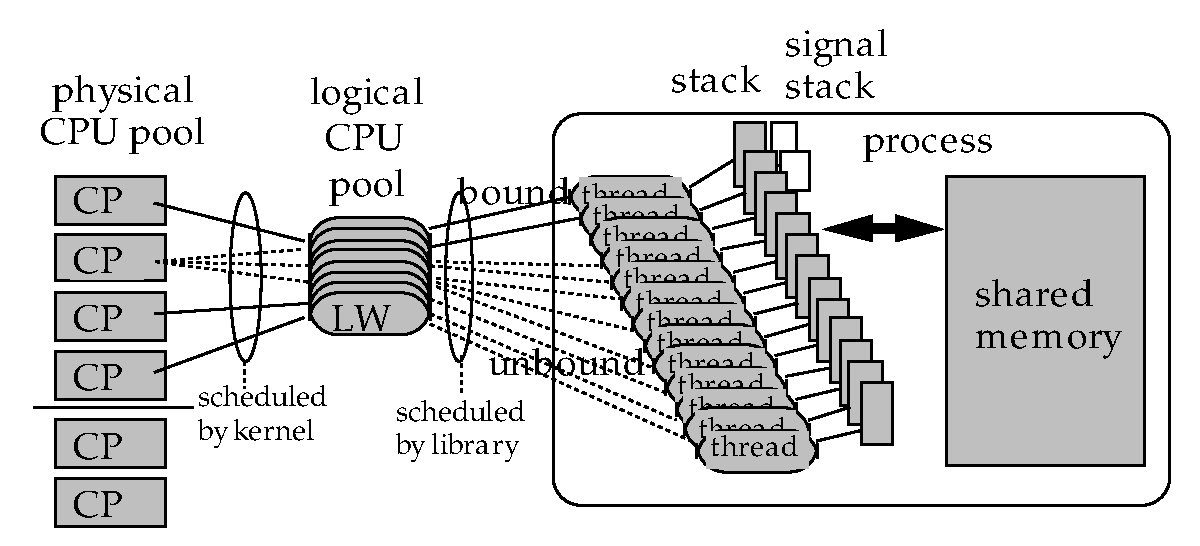
\includegraphics[width=13cm]{fig/threadfig.ps}
%\mbox{
%\epsfxsize=13cm
%\epsfbox{fig/threadfig.ps}
%}

\caption{Solaris operating system's thread model}\label{threadmodel}
\end{center}
\end{figure}

A context consists of a C-stack, a binding-stack and frame 
pointers that chain lexical blocks such as {\tt lambda, block, catch,
let, flet}, and so on,  and is established when a new thread
is created. Since more than one context can be active at
the same time on a real multi-processor machine, we cannot
hold a single pointer to the current context in a global variable.
Rather we have to add one more argument to every internal
function to transfer the context pointer  from the topmost eval
to the memory manager at the bottom.

\subsubsection{Memory Management}
EusLisp adopts a Fibonacci buddy memory management scheme in a
single heap for every type of object. 
After running programs having
different memory request characteristics, we have been convinced that
Fibonacci buddy can allocate objects of various sizes equally fast,
garbage-collects quickly without copying , and exhibits high memory
utilization (the internal loss is 10 to 15\% and the
external loss is negligible).
For multithreading, the second point, i.e., non-copying GC, is very
important.
If addresses of objects were changed by copying-GC, pointers in the
stack and CPU registers of all thread contexts would have to be
redirected to new locations, which is impossible or very difficult. 

All memory allocation requests are handled by the {\tt alloc} function at the
lowest level.
{\tt Alloc} does mutex-locking because it manipulates the global
database of free lists.
Since we cannot predict when a garbage
collection begins and which thread causes it, every thread must prepare
for sporadic GCs.  All pointers to living objects have to be arranged
to be accessible by the GC anytime to prevent them from being reclaimed
as garbage.  This is done by storing the pointers to the most recently
allocated objects in fixed slots of each context, instead of trusting
they are maintained on the stacks.

Fig. \ref{parathreads} illustrates flow of threads requesting memory and forked inside
GC to process marking and sweeping in parallel.
Note that threads that do not request memory or manipulate pointers
can run in parallel with the GC,
improving real-time response of the low-level tasks such as signal
processing and image acquisition.

\begin{figure}
\begin{center}
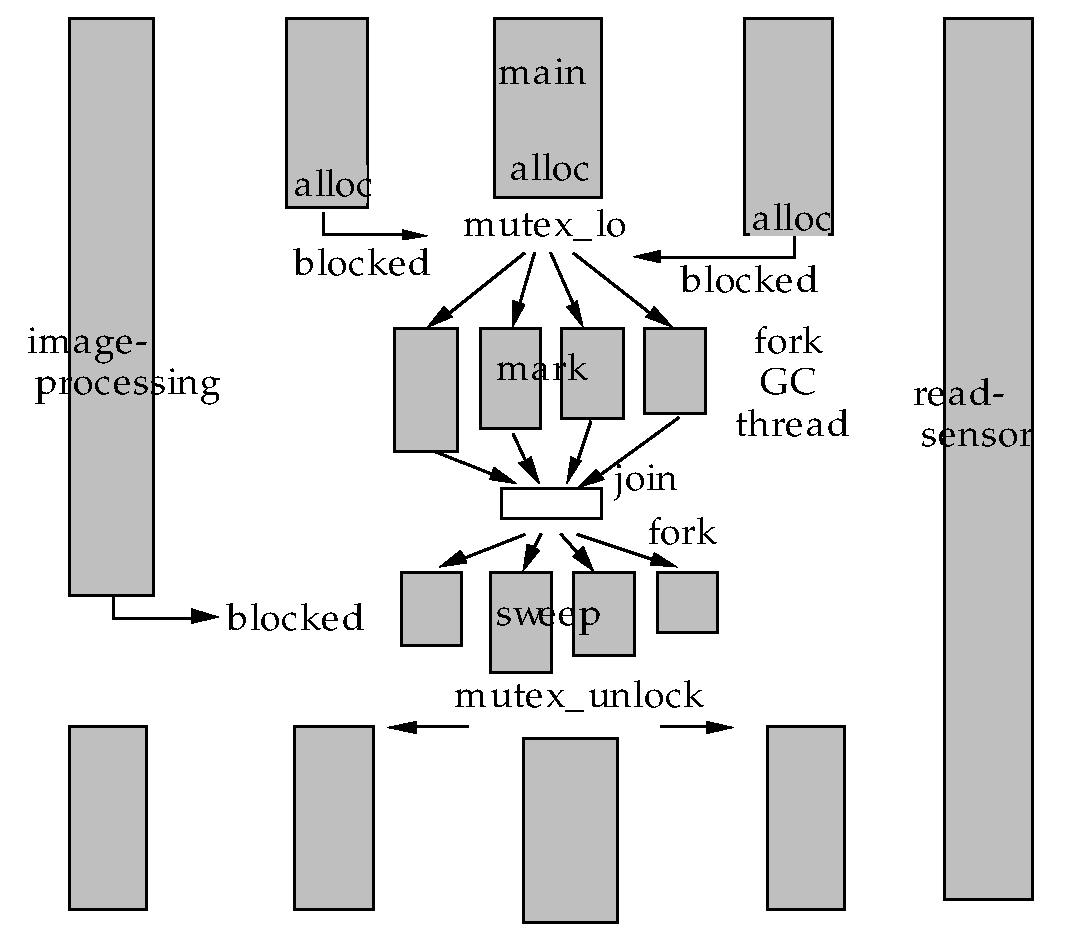
\includegraphics[width=120mm]{fig/parathreads.ps}
%\epsfile{file=fig/parathreads.ps,width=120mm}
\caption{Parallel threads requesting memory and GC running in parallel}\label{parathreads}
\end{center}
\end{figure}

\subsection{Asynchronous and Parallel Programming Constructs}
\subsubsection{Thread Creation and Thread Pool}
In order for Solaris to execute a program in parallel on many
processors, the program needs to be written as a collection
of functions, each of which is executed by a thread dynamically
created in a process.  Although the time required for thread
creation is faster than process creation, it takes a few
mili-seconds for EusLisp to start off a thread after allocating
stacks and setting a page attribute for detecting stack-overflow.
Since this delay, which should be compared to a function invocation,
is intolerable, sufficient number of threads are created by
the {\tt make-thread} function beforehand and put in 
the system's thread pool,
eliminating the need for system calls at evaluation time.
Each thread in the thread pool is represented by a thread object,
as depicted in Fig.\ref{threadobj},
consisted of thread-id, several semaphores for synchronization,
and slots for argument and evaluation result transfer.

\begin{figure}
\begin{center}
\begin{tabular}{c c}
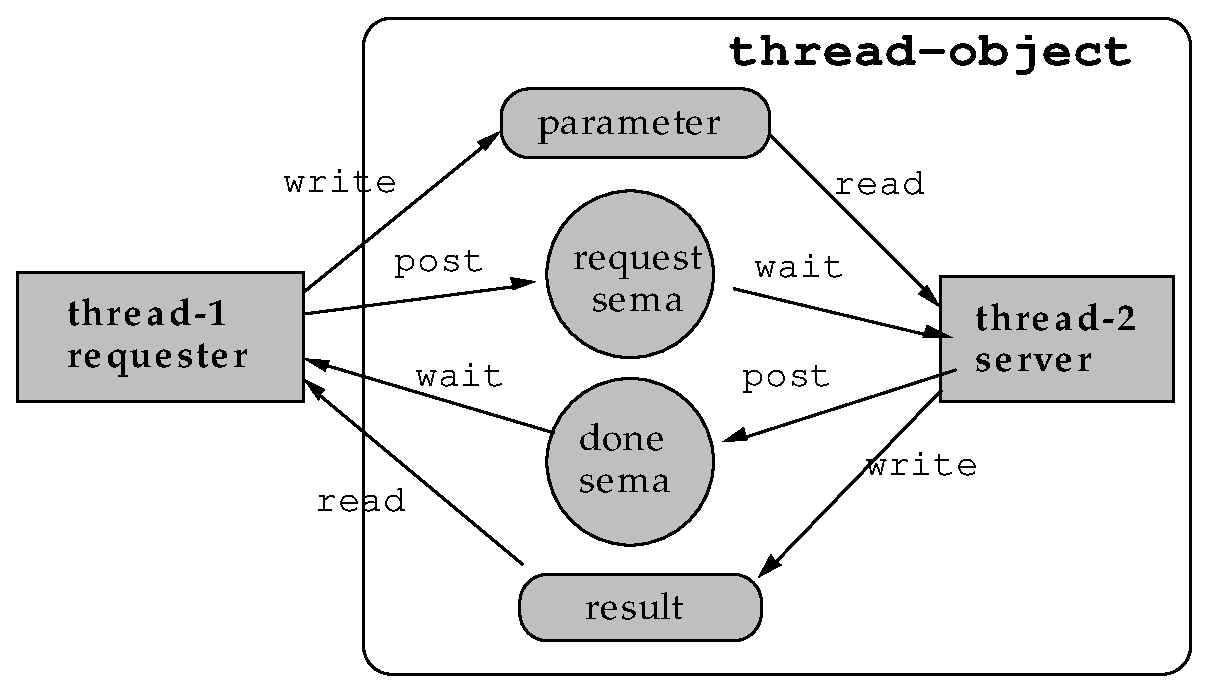
\includegraphics[width=7.5cm]{fig/threadobj.ps} &
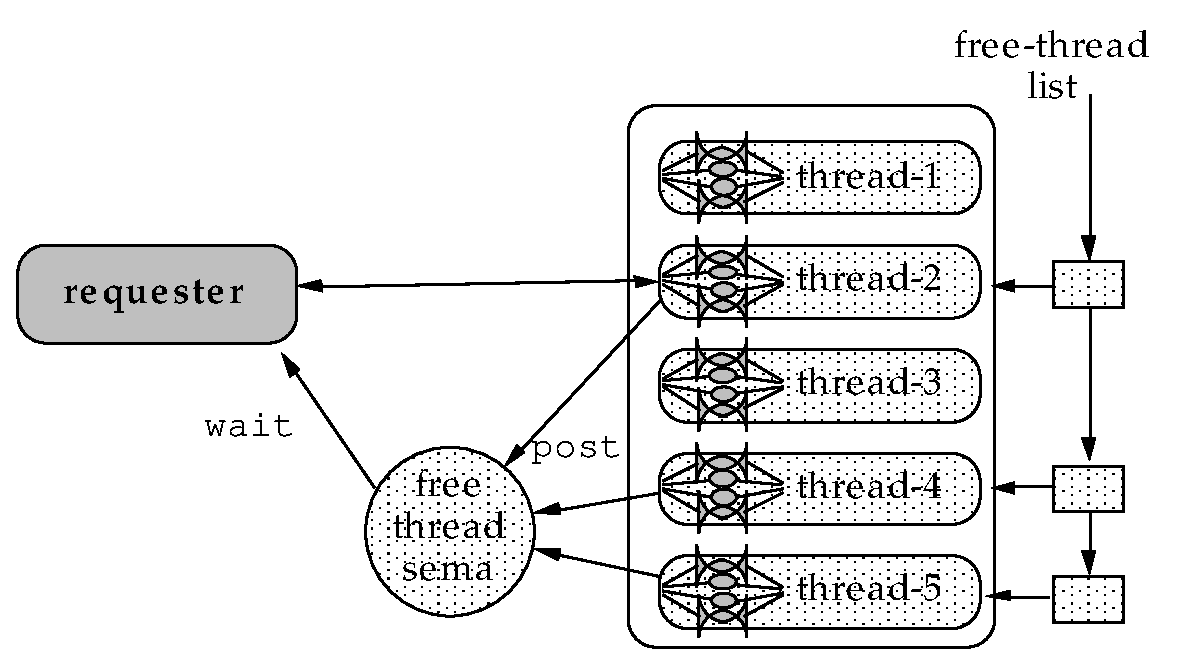
\includegraphics[width=7.5cm]{fig/threadpool.ps} \\
%\epsfile{file=fig/threadobj.ps,width=7.5cm} &
%\epsfile{file=fig/threadpool.ps,width=7.5cm} \\
\end{tabular}
\end{center}
\caption{\label{threadobj}Thread-object for transferring control and data between threads (left) and the collection of threads put in the thread-pool.}
\end{figure}

\subsubsection{Parallel Execution of Threads}
For the allocation of parallel computation to threads, the thread function
is used.
Thread takes one free thread out of the thread pool,
transfers arguments via shared memory, wakes up the thread by signaling
the semaphore as indicated in fig. \ref{threadobj},
and returns a thread object to the caller without blocking.
The woken-up thread begins evaluation of
the argument running in parallel to the calling thread.
The caller uses
{\tt wait-thread} to receive the evaluation result from the forked thread.
The {\tt plist} macro is a more convenient form to describe parallel 
evaluation of arguments.
{\tt Plist} attaches threads to evaluate each argument
and lists up results after waiting for all threads to finish evaluation.

\subsubsection{Synchronization primitives}
MT-Eus has three kinds of synchronization primitives,
namely {\em mutex locks, condition variables}, and {\em semaphores}.
Mutex locks  are used to serialize accesses to shared variables
between threads.
Condition variables allow a thread to wait for a condition to become
true in a mutex-locked section by temporarily releasing and re-acquiring 
the lock.
Semaphores are used to inform occurrences of events, or to control
sharing of finite resources.
These synchronization primitives cause voluntary context switching,
while the Solaris kernel generates involuntary task switching
on a time-sliced scheduling basis.

\begin{figure}
\begin{center}
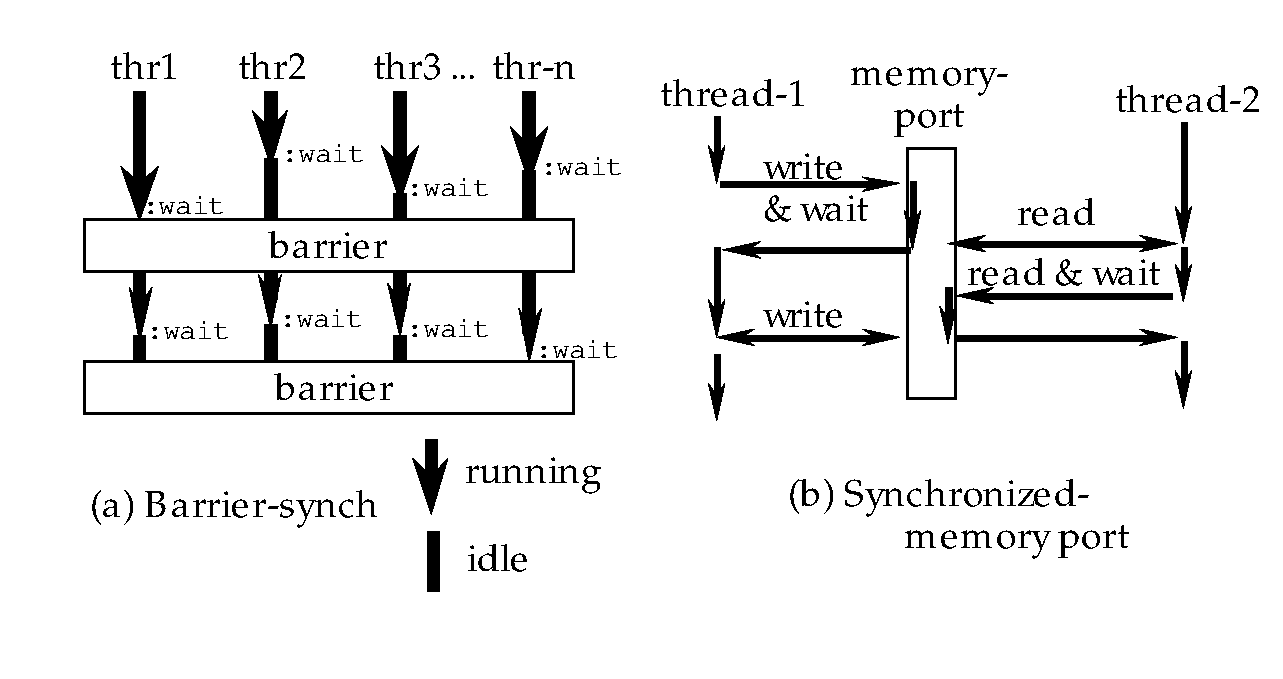
\includegraphics[width=130mm]{fig/synchports.ps}
%\epsfile{file=fig/synchports.ps,width=130mm}
\caption{Barrier synchronization and synchronozed memory port}
\label{synchports}
\end{center}
\end{figure}

\subsubsection{Barrier synchronization}
{\em Barrier-synch} is a mechanism for more than two threads to synchronize
at the same time (Fig. \ref{synchports}).
For this purpose, an instance of the barrier class
is created and threads that participate in
the synchronization register themselves in the object.
Then, each thread sends the {\tt :wait} message to the barrier object,
and the thread is blocked.
When the last thread registered in the object sends its
{\tt :wait} message, the waits are released and all waiting
threads get a return value of T.
Barrier-sync plays an important role of global clocking in a
multi-robot simulation.

\subsubsection{Synchronized memory port}
Synchronized memory port is a kind of stream to exchange data
between threads (Fig. \ref{synchports}).
Since all threads in a process share the
heap memory, if one thread binds an object to a global variable,
it  instantly becomes visible to other threads.
However, shared memory lacks capability to send events that the
global data is updated. Synchronized memory port ensures this 
synchronization for accessing a shared object. A synchronized
memory port object consists of one buffer slot and two semaphores
used for synchronizing  read and write.

\subsubsection{Timers}
Real-time programs often require functions to execute at
predetermined timing or to repeat in particular intervals.
Sequential EusLisp could run user' functions triggered by
signals generated periodically by Unix's interval timers.
This preemption can cause deadlock in MT-Eus,
because interruption may occur within a mutex-ed block.
Therefore, control must be transferred at secured points
such as at the beginning of {\tt eval}.
To avoid delays caused by the above synchronization,
MT-Eus also provides signal-notification via semaphores.
In other words, the signal function takes either a function or
a semaphore that is called or posted upon the signal arrival.
Since the semaphore is posted at the lowest level, latency
for synchronization is minimal.

The following a example image processing program
coded by using the multithread facilities.
Image input thread and filtering
threads are created. samp-image takes image data periodically
by waiting for samp-sem to be posted every 33msec.
Two threads synchronize via read-and-write of a thread-port.
Filter-image employs two more threads for parallel computation
of filtering.

\begin{quote}
\begin{verbatim}
(make-threads 8)
(defun samp-image (p)
   (let ((samp-sem (make-semaphore)))
        (periodic-sema-post 0.03 samp-sem)
        (loop (sema-wait samp-sem)
              (send p :write (read-image))))
(defun filter-image (p)
  (let (img)
       (loop (setf img (send p :read))
             (plist (filter-up-half img)
                    (filter-low-half img)))))
(setf port (make-thread-port))
(setf sampler (thread #'samp-image port))
(setf filter (thread #'filter-image port))
\end{verbatim}
\end{quote}

\subsection{Measured Parallel Gains}

Table. \ref{paragain} shows the parallel execution performance
measured on a Cray Supserserver configured with 32 CPUs.
Linear parallel gain was obtained for the compiled Fibonacci function,
because there is no shared memory access and  the program code
is small enough to be fully loaded onto the cache memory of
each processor.
Contrally, when the same program was interpreted, linearly
high performance could not be attained, since memory access
scatters. Further, some programs that frequently refer to 
shared memory and request memory allocation cannot exhibit better
performance than a single processor execution.
This can be understood as the result of frequent  cache memory
purging.

\begin{table}
\begin{center}
\begin{tabular}{|l|r|r|r|r|c|}  \hline
processors & 1 & 2 & 4 & 8 & GC (ratio) \\ \hline
(a) compiled Fibonacci & 1.0 & 2.0 & 4.0 & 7.8 & 0 \\ \hline
(b) interpreted Fibonacci & 1.0 & 1.7 & 2.7 & 4.4 & 0 \\ \hline
(c) copy-seq & 1.0 & 1.3 & 0.76 & 0.71 & 0.15 \\ \hline
(d) make-cube & 1.0 & 0.91 & 0.40 & 0.39 &  0.15 \\ \hline
(e) interference-check & 1.0 & 0.88 & 0.55 & 0.34 & 0.21 \\ \hline
\end{tabular} \\
\caption{\label{paragain}Parallel gains of programs executed on multi-processors}
\end{center}
\end{table}

\subsection{Thread creation}
A thread is a unit for assigning computation, usually evaluation
of a lisp form.
Threads in EusLisp are represented by instances of
the {\bf thread} class.
This object is actually a control port of a thread 
to pass arguments and result, and let it start evaluation,
rather than the thread's entity representing the context.

\begin{refdesc}

\funcdesc{sys:make-thread}{num \&optional (lsize 32*1024) (csize lsize)}{
creates {\em num} threads with {\em lsize} words of Lisp stack
and {\em csize} words of C stack, and put them in the system's
thread pool.
All the threads in the thread pool is bound to sys:*threads*,
which is extended each time {\bf make-thread} is called.
By the {\bf thread} function, a computation is assigned to one
of free threads in the thread pool.
Therefore it is not a good idea to change stack sizes
from thread to thread,
since you cannot control which thread is assigned to a specific
computation.}

\vardesc{sys:*threads*}{
returns the list of all the threads created by {\bf make-threads}.}

\funcdesc{sys::free-threads}{}{
returns the list of threads in the
free thread pool.
If the result is NIL, new commitment of a task to a thread
is blocked until any currently running threads finish evaluation
or new threads are created by {\bf make-thread} in the free thread pool.}

\funcdesc{sys:thread}{func \&rest args}{
picks up one free thread from the thread pool, and assigns it
for evaluation of {\em (func . args)}.
{\bf Sys:thread} can be regarded as asynchronous {\bf funcall},
since {\bf sys:thread} applies {\em func} to the spread list
of {\em args} but it does not accept the result of the
function application.
Rather, {\bf sys:thread} returns the thread object assigned to
the funcall, so that the real result can be obtained later
by {\bf sys:wait-thread}.}
\begin{quote}
\begin{verbatim}
(defun compute-pi (digits) ...)
(setq trd (sys:thread \#'compute-pi 1000)) ;assign compute-pi to a thread
...  ;; other computation 
(sys:wait-thread trd) ;get the result of (compute-pi 1000)
\end{verbatim}
\end{quote}

\funcdesc{sys:thread-no-wait}{func \&rest args}{
assigns computation to one of free threads.
The thread is reclaimed in the free thread pool when
it finishes evaluation without being {\bf wait-thread}'ed.}

\funcdesc{sys:wait-thread}{thread}{
waits for {\em thread} to finish evaluation of funcall given
by the {\bf sys:thread} function, and retrieves the result
and returns it.
{\bf Sys:wait-thread} is mandatory if the thread is assigned
evaluation by {\bf sys:thread} because the thread is not returned
to the free thread pool until it finishes transferring the result.}
 
\macrodesc{sys:plist}{\&rest forms}{evaluates {\em forms} by different
threads in parallel and waits for the completion of all evaluation,
and the list of results is returned.
{\bf Sys:plist} may be regarded as {\em parallel-list} except that
each form listed must be a function call.}


\end{refdesc}

\subsection{Synchronization}

Among Solaris operating systems four synchronization primitives for
multithread programs, EusLisp provides mutex locks, conditional variables,
and semaphores. Reader-writer lock is not available now.

Based on these primitives, higher level synchronization mechanisms,
such as synchronized memory port and barrier synchronization, are realized.

\begin{refdesc}
\funcdesc{sys:make-mutex-lock}{}{
makes a mutex-lock and returns it. A mutex-lock is represented by an
integer-vector of six elements.}
\funcdesc{sys:mutex-lock}{mlock}{
locks the mutex lock {\em mlock}.
If the {\em mlock} is already locked by another thread,
{\em mutex-lock} waits for the lock to be released.}

\funcdesc{sys:mutex-unlock}{mlock}{
releases {\em mlock} and let one of other threads waiting for this
lock resume running.}

\macrodesc{sys:mutex}{mlock \&rest forms}{
Mutex-lock and mutex-unlock have to be used as a pair.
{\bf Mutex} is a macro that brackets a critical section.
{\em Mlock} is locked
before evaluating {\em forms} are evaluated,
and the lock is released when the evaluation finishes.
This macro expands to the following progn form.
Note that {\bf unwind-protect} is used to ensure unlocking
even an error occurs during the evaluation of {\em forms}.
}
\begin{quote}
\begin{verbatim}
  (progn
      (sys:mutex-lock mlock)
      (unwind-protect
          (progn . forms)
          (sys:mutex-unlock mlock)))
\end{verbatim}
\end{quote}

\funcdesc{sys:make-cond}{}{makes a condition variable object
which is an integer vector of four elements.
The returned condition variable is in unlocked state.}

\funcdesc{sys:cond-wait}{condvar mlock}{
waits for {\em condvar} to be signaled.
If {\em condvar} has already been acquired by another thread,
it releases {\em mlock} and waits for {\em condvar} to be signaled.}
\funcdesc{sys:cond-signal}{condvar}{signals the {\em condvar} condition variable.}
\funcdesc{sys:make-semaphore}{}{makes a semaphore object
which is represented by an integer vector of twelve elements.}
\funcdesc{sys:sema-post}{sem}{ signals {\em sem}.}
\funcdesc{sys:sema-wait}{sem}{waits for the {\em sem} semaphore to be posted.}

\classdesc{sys:barrier-synch}{propertied-object}{
threads n-threads count barrier-cond threads-lock count-lock}
{represents a structure for barrier-synchronization. Threads waiting
for the synchronization are put in {\em threads} which is mutually excluded
by {\em threads-lock}.
When a {\bf barrier-synch} object is created,
{\em count} is initialized to zero.
Synchronizing threads are put in the {\em threads} list by sending {\tt :add}
message.
Sending {\tt :wait} to this barrier-sync object causes {\em count} to be
incremented, and the sending thread is put in the wait state.
When all the threads in {\em threads} send the {\tt :wait} message,
the waits are unblocked and all threads resume execution.
The synchronization is implemented by the combination of
the {\em count-lock} mutex-lock and the {\em barrier-cond}
condition-variable.}

\methoddesc{:init}{}{initializes this barrier-synch object. Two mutex-lock
and one condition-variable are created.}
\methoddesc{:add}{thr}{adds the {\em thr} thread in the {\em threads} list.}
\methoddesc{:remove}{thr}{removes the {\em thr} thread of the {\em threads} list.}
\methoddesc{:wait}{}{waits for all threads in the {\em threads} list
to issue {\tt :wait}.}

\classdesc{sys:synch-memory-port}{propertied-object}{
sema-in sema-out buf empty lock}{
realizes the one-directional synchronized memory port,
which synchronizes for two threads
to transfer datum via this object.
Control transfer is implemented by using semaphores.}

\methoddesc{:read}{}{reads datum buffered in this synch-memory-port.
If it has not been written yet, the :read blocks.}
\methoddesc{:write}{datum}{writes {\em datum} in the buffer.
Since only one word of buffer is available,
if another datum has already been written and not yet read out,
:write waits for the datum to be transferred by :read.}
\methoddesc{:init}{}{initializes this synch-memory-port
where two semaphores  are created and :write is made acceptable.}

\end{refdesc}

\markboth{EusLisp version \eusversion Reference Manual (Part III)}{Geometric/Robot Functions}
\newpage
\section{Geometric Functions}
\markright{\arabic{section}. Geometric Functions}

\subsection{Float-vectors}

A float-vector is a simple vector whose elements are specialized to
floating point numbers.
A float-vector can be of any size.
When {\em result} is specified in an argument list,
it should be a float-vector that holds the result.

\begin{refdesc}

\funcdesc{float-vector}{\&rest numbers}{
makes a new float-vector whose elements are {\em numbers}.
Note the difference between {\tt (float-vector 1 2 3)} and {\tt \#F(1 2 3)}.
While the former create a vector each time it is called, the latter
does when it is read.}

\funcdesc{float-vector-p}{obj}{
returns T if {\em obj} is a float-vector.}

\funcdesc{v+}{fltvec1 fltvec2 \&optional result}{
adds two float-vectors.}

\funcdesc{v-}{fltvec1 \&optional fltvec2  result}{
subtract float-vectors. If fltvec2 is omitted, fltvec1 is negated.}

\funcdesc{v.}{fltvec1 fltvec2}{computes the inner product of two float-vectors.}

\funcdesc{v*}{fltvec1 fltvec2 \&optional result}{
computes the outer product of two float-vectors.}

\funcdesc{v.*}{fltvec1 fltvec2 fltvec3}{
computes the scaler triple product [A,B,C]=(V. A (V* B C))=(V. (V* A B) C).}

\funcdesc{v$<$}{fltvec1 fltvec2}{
returns T if every element of fltvec1 is smaller  than
the corresponding element of fltvec2.}

\funcdesc{v$>$}{fltvec1 fltvec2}{
returns T if every element of fltvec1 is larger than
the corresponding element of fltvec2.}

\funcdesc{vmin}{\&rest fltvec}{
finds the smallest values for each dimension in {\em fltvec},
and makes a float-vector from the values.
{\bf Vmin} and {\bf vmax} are used to find the minimal bounding box
from coordinates of vertices.}

\funcdesc{vmax}{\&rest fltvec}{
finds the greatest values for each dimension in {\em fltvec},
and makes a float-vector from the values.}

\funcdesc{minimal-box}{v-list minvec maxvec [err]}{
computes the minimal bounding box for a given vertex-list,
and stores results in {\em minvec} and {\em maxvec}.
If a floating number err is specified, the minimal box is grown
by the ratio, i.e. if the err is 0.01, each element of minvec is decreased
by 1\% of the distance between minvec and maxvec,
and each element of maxvec is increased by 1\%.
{\bf Minimal-box} returns the distance between minvec and maxvec.}

\funcdesc{scale}{number fltvec \&optional result}{
the scaler {\em number} is multiplied to the every element of fltvec.}

\funcdesc{norm}{fltvec}{$|fltvec|$}
\funcdesc{norm2}{fltvec}{$|fltvec|^2=({\bf v.} fltvec fltvec)$}
\funcdesc{normalize-vector}{fltvec [result]}{
normalizes {\em fltvec} to have the norm 1.0.}
\funcdesc{distance}{fltvec1 fltvec2}{
returns the distance $|fltvec-fltvec2|$ between two float-vectors.}
\funcdesc{distance2}{fltvec1 fltvec2}{
$|fltvec-fltvec2|^2$}

\funcdesc{homo2normal}{homovec \&optional normalvec}{
A homogeneous vector {\em homovec} is converted to its normal representation.}

\funcdesc{homogenize}{normalvec \&optional homovec}{
A normal vector {\em normalvec} is converted to its homogenous representation.}

\funcdesc{midpoint}{p p1 p2 \&optional result}{
{\em P} is float, and {\em p1} and {\em p2} are float-vectors of the same
dimension.
A point $(1-p) p1 + p p2$, which is the point
that breaks {\em p1-p2} by the ratio $p:(1-p)$, is returned.}

\funcdesc{rotate-vector}{fltvec theta axis \&optional result}{
rotates 2D or 3D {\em fltvec} by {\em theta} radian around {\em axis}.
{\em Axis} can be one of {\em :x, :y, :z, 0, 1, 2} or NIL.
When {\em axis} is NIL, {\em fltvec} is taken to be two dimensional.
To rotate a vector around an arbitrary axis in 3D space, 
make a rotation matrix by the {\bf rotation-matrix} function and
multiply it to the vector.}

\end{refdesc}

\subsection{Matrix and Transformation}

A matrix is a two-dimensional array whose elements are all floats.
In most functions a matrix can be of any size,
but the {\bf v*, v.*}, {\bf Euler-angle} and {\bf rpy-angle} functions
can only handle three dimensional matrices.
{\bf Transform, m*} and {\bf transpose} do not restrict
the matrices to be square,
and they operate on general n*m size matrices.

Functions that can accept result parameter
places the computed result there, and no heap is wasted.
All matrix functions are intended for the transformation in the normal
coordinate systems, and not in the homogeneous coordinates.

The {\bf rpy-angle} function decomposes a rotation matrix into three components
of rotation angles around z, y and x axes of the world coordinates.
The {\bf Euler-angle} function is similar to {\bf rpy-angle} but
decomposes into rotation angles around local z, y and again z axes.
Both of these functions return two solutions since angles can be
taken in the opposite directions.

\begin{verbatim}
; Mat is a 3X3 rotation matrix.
(setq rots (rpy-angle mat))
(setq r (unit-matrix 3))
(rotate-matrix r (car rots) :x t r)
(rotate-matrix r (cadr rots) :y t r)
(rotate-matrix r (caddr rots) :z t r)
;--> resulted r is equivalent to mat
\end{verbatim}

To keep track of pairs of a position and a orientation in 3D space, use
the {\bf coordinates} and {\bf cascaded-coords} classes
detailed in the section \ref{Coordinates}.

\begin{refdesc}
\funcdesc{matrix}{\&rest elements}{
makes a new matrix from {\em elements}.
Row x Col = (number of elements) x (length of the 1st element).
Each of {\em elements} can be of any type of sequence.
Each sequence is lined up as a row vector in the matrix.}

\funcdesc{make-matrix}{rowsize columnsize \&optional init}{
makes a matrix of $rowsize \times columnsize$.}

\funcdesc{matrixp}{obj}{
T if {\em obj} is a matrix, i.e. {\em obj} is a two dimensional array
and its elements are floats.}

\funcdesc{matrix-row}{mat row-index}{
extracts a row vector out of matrix {\em mat}.
{\bf matrix-row} is also used to set a vector in a particular row
of a matrix using in conjunction with {\bf setf}.}
\funcdesc{matrix-column}{mat column-index}{
extracts a column vector out of {\em mat}.
{\bf matrix-column} is also used to set a vector in a particular
column of a matrix using in conjunction with {\bf setf}.}
\funcdesc{m*}{matrix1 matrix2 \&optional result}{
concatenates {\em matrix1} and {\em matrix2}.}
\funcdesc{transpose}{matrix \&optional result}{
transposes {\em matrix}, i.e. columns of {\em matrix} are exchanged with
{\em rows}.}
\funcdesc{unit-matrix}{dim}{
makes an identity matrix of {\em dim} $\times$ {\em dim}.}
\funcdesc{replace-matrix}{dest src}{
replaces all the elements of dest matrix with ones of src matrix.}

\funcdesc{scale-matrix}{scalar mat}{
multiplies {\em scaler} to all the elements of {\em mat}.}

\funcdesc{copy-matrix}{matrix}{
makes a copy of {\em matrix}.}

\funcdesc{transform}{matrix fltvector \&optional result}{
multiplies {\em matrix} to {\em fltvector} from the left.}
\funcdesc{transform}{fltvector matrix \&optional result}{
multiplies {\em matrix} to {\em fltvector} from the right.}

\funcdesc{rotate-matrix}{matrix theta axis \&optional world-p result}{
multiplies a rotation matrix from the left (when world-p is non-nil)
or from the right (when world-p is nil).
When a matrix is rotated by {\bf rotate-matrix},
the rotation axis {\bf :x, :y, :z} or 0,1,2
may be taken either in the world coordinates or in the local coordinates.
If {\em world-p} is specified nil, it means rotation along the
axis in the local coordinate system and the rotation matrix is multiplied
from the right.
Else if worldp is non-nil, the rotation is made in the
world coordinates and the rotation matrix is multiplied from the left.
If NIL is given to {\em axis}, {\em matrix} should be two dimensional and
the rotation is taken in 2D space where {\em world-p} does not make sense.}

\funcdesc{rotation-matrix}{theta axis \&optional result}{
makes a 2D or 3D rotation matrix around {\em axis} which can be any of
:x, :y, :z, 0, 1, 2, a 3D float-vector or NIL.
When you make a 2D rotation matrix, axis should be NIL.}

\funcdesc{rotation-angle}{rotation-matrix}{
extracts a equivalent rotation axis and angle from {\em rotation-matrix}
and a list of float and float-vector is returned.
NIL is returned when {\em rotation-matrix} is a unit-matrix.
Also if the rotation angle is too small, the result may have errors.
When {\em rotation-matrix} is 2D,  the single angle value is returned.}

\funcdesc{rpy-matrix}{ang-z ang-y ang-x}{
makes a rotation matrix defined by roll-pitch-yaw angles.
First, a unit-matrix is rotated by ang-x radian along X-axis.
Next, ang-y around Y-axis and finally ang-z around Z-axis.
All the rotation axes are taken in the world coordinates.}

\funcdesc{rpy-angle}{matrix}{
extracts two triplets of roll-pitch-yaw angles of {\em matrix}.}

\funcdesc{Euler-matrix}{ang-z ang-y ang2-z}{
makes a rotation matrix defined by three Euler angles.
First, a unit-matrix is rotated {\em ang-z} around Z-axis, next, {\em ang-y}
around Y-axis and finally {\em ang2-z} again around Z-axis.
All the rotation axes are taken in the local coordinates.}

\funcdesc{Euler-angle}{matrix}{
extracts two tuples of Euler angles.}

%\funcdesc{set-matrix-row}{mat row-index values}{
%puts values in the {\em row-index}th row of matrix {\em mat}.}

%\funcdesc{set-matrix-column}{mat column-index values}{
%put values in the {\em column-index}th column of of matrix {\em mat}.}
\end{refdesc}

\subsection{LU decomposition}
{\bf lu-decompose} and {\bf lu-solve} are provided to solve
simultaneous linear equations.
First, {\bf lu-decompose} decomposes a matrix into a lower triangle matrix
and an upper triable matrix.
If the given matrix is singular, {\bf LU-decompose} returns NIL, otherwise
it returns the permutation vector which should be supplied to {\bf LU-solve}.
{\bf Lu-solve} computes the solution for a LU matrix with a given constant vector.
This method is efficient if solutions for many combinations 
of different constant vectors and the same factor matrix are required.
%These functions are coded in C, and they computes a solution
%for a 3*3 matrix within 3 milli-sec on sun3.
{\bf Simultaneous-equation} would be  more handy when you wish to get
only one solution.
{\bf Lu-determinant} computes a determinant of a lu-decomposed matrix.
{\bf Inverse-matrix} function computes an inverse matrix using {\bf lu-decompose}
once, and {\bf lu-solve} n times.
Computation time for a 3*3 matrix is estimated to be 4 milli-sec.

\begin{refdesc}

\funcdesc{lu-decompose}{matrix \&optional result}{
performs lu-decomposition of {\em matrix}.}

\funcdesc{lu-solve}{lu-mat perm-vector bvector [result]}{
solves a linear simultaneous equations which has already been lu-decomposed.
{\em perm-vector} should be the result returned by {\bf lu-decompose}.}

\funcdesc{lu-determinant}{lu-mat perm-vector}{
computes the determinant value for a matrix which has already been 
lu-decomposed.}

\funcdesc{simultaneous-equation}{mat vec}{
solves a linear simultaneous equations whose coefficients are described in
{\em mat} and constant values in {\em vec}.}

\funcdesc{inverse-matrix}{mat}{
makes the inverse matrix of the square matrix, {\em mat}.}

\funcdesc{pseudo-inverse}{mat}{
computes the pseudo inverse matrix using the singular value decomposition.}

\end{refdesc}

\newpage

\subsection{\label{Coordinates}Coordinates}

Coordinate systems and their transformations are represented by
the {\bf coordinates} class.
Instead of 4*4 (homogeneous) matrix representation,
coordinate system in EusLisp is represented by a combination of
a 3*3 rotation matrix and a 3D position vector
mainly for speed and generality.

\begin{refdesc}

\classdesc{coordinates}{propertied-object}
{(pos :type float-vector \\
\>  rot :type array)}
{defines a coordinate system with a pair of a position vector and a 3x3
rotation matrix.}

\funcdesc{coordinates-p}{obj}{
returns T when obj is an instance of coordinates class or its subclasses.}

\methoddesc{:rot}{}{
returns the 3X3 rotation matrix of this coords.}

\methoddesc{:pos}{}{
returns the 3-D position vector of this coords.}

\methoddesc{:newcoords}{newrot &optional newpos}{
updates the coords with newrot and newpos. Whenever a condition that changes
the state of this coords occurs,
this method should be called with the new rotation
matrix and the position vector.
This message may invoke another :update method to propagate the event.
If newpos is not given, newrot is given as a instance of coordinate class.
}

\methoddesc{:replace-coords}{newrot &optional newpos}{
changes the rot and pos slots to be updated without calling newcoords method.
If newpos is not given, newrot is given as a instance of coordinate class.
}

\metdesc{:coords}{}

\methoddesc{:copy-coords}{\&optional dest}{
If dest is not given, :copy-coords makes another coordinates object
which has the same rot and pos slots. If dest is given, rot and pos of
this coordinates is copied to the dest coordinates.}

\methoddesc{:reset-coords}{}{
forces the rotation matrix of this coords to be identity matrix, and pos
vector to be all zero.}

\metdesc{:worldpos}{}
\metdesc{:worldrot}{}
\methoddesc{:worldcoords}{}{
Computes the position vector, the rotation matrix and the coordinates
of this object represented in the world coordinates. The coordinates class
is always assumed to be represented in world, these method can simply return
pos, rot and self.  These methods are provided for the compatibility with
cascaded-coords class which cannot be assumed to be represented in world.}

\methoddesc{:copy-worldcoords}{\&optional dest}{
First, worldcoords is computed, and it is copied to dest. If no dest
is specified, a coordinates object to store the result is newly created.}

\methoddesc{:rotate-vector}{vec}{
A vector is rotated by the rotation of this coords, i.e., an orientation
vector represented in this coords is converted to the representation
in the world.
The position of this coords does not affect rotation.}

\methoddesc{:transform-vector}{vec}{
A vector in this local coords is transformed to the representation in the world.}

\methoddesc{:inverse-transform-vector}{vec}{
A vector in the world is inversely transformed to the representation in this
local coordinate system.}

\methoddesc{:transform}{ trans \&optional (wrt :local)}{
Transform this coords by the trans represented in wrt coords.
Trans must be of type coordinates, and wrt must be one of keywords
{\tt :local, :parent, :world} or an instance of coordinates.
If wrt is {\tt :local}, the trans is applied from the right to this coords,
and if wrt is {\tt :world} or {\tt :parent},
the trans is multiplied from the left.
Else, if wrt is of type coordinates, the trans represented in the wrt
coords is first transformed to the representation in the world, and  it
is applied from the left.}

\methoddesc{:move-to}{trans \&optional (wrt :local)}{
Replaces the rot and pos of the coords with trans represented in wrt.}

\methoddesc{:translate}{ p \&optional (wrt :local)}{
changes the position of this object
relatively with respective to wrt coords.}

\methoddesc{:locate}{ p \&optional (wrt :local)}{
Changes the location of this coords with the parameter represented in wrt.
If wrt is {\tt :local}, then the effect is identical to 
{\bf :translate} with {\em wrt}={\tt :local}.}

\methoddesc{:rotate}{ theta axis \&optional (wrt :local)}{
Rotates this coords relatively by {\em theta} radian around the {\em axis}.
{\em Axis} is one of axis-keywords ({\tt :x, :y} and {\tt :z}) or an arbitrary float-vector.
{\em Axis} is considered to be represented in the {\em wrt} coords.
Thus, if {\em wrt}={\tt :local} and {\em axis}={\tt :z},
the coordinates is rotated around the z
axis of this local coords, and {\em wrt}={\tt :world} or {\tt :parent},
the coords is rotated around the z axis of world coords.
In other words, if {\em wrt}={\tt :local},
a rotation matrix is multiplied from the right of this coords,
and if {\em wrt}={\tt :world} or {\tt :parent},
a rotation matrix is multiplied from the left.
Note that even {\em wrt} is either {\tt :world} or {\tt :parent},
the {\em pos} vector of this coordinates does not change.
For the true rotation around the world axis,
an instance of coordinates class representing the
rotation should be given to {\bf :transform} method.}

\methoddesc{:orient}{ theta axis \&optional (wrt :local)}{
forces setting rot.
This is an absolute version of :{\bf rotate} method.}

\methoddesc{:inverse-transformation}{}{
makes a new coords that is inverse to self.}

\methoddesc{:transformation}{ coords (wrt :local)}{
makes the transformation (an instance of coordinates) between this coords
and the coords given as the argument.
If {\em wrt}={\tt :local},
the result is represented in local coords,
i.e., if the resulted transformation is given
as an argument to :transform with {\em wrt}={\tt :local},
this coords is transformed
to be identical with the coords.}

\methoddesc{:Euler}{ az1 ay az2}{
sets rot with Euler angles, that are,
rotation angles around z ({\em az1},
y ({\em ay}) and again z {\em az2} axis of
this local coordinates system.}

\methoddesc{:roll-pitch-yaw}{roll pitch yaw}{
sets rot with roll-pitch-yaw angles:
rotation angles around x ({\em yaw}), y ({\em pitch}) and z ({\em roll})
axes of the world coordinate system.}

\methoddesc{:4x4}{\&optional mat44}{
If a matrix of 4x4 is given as {\em mat44},
it is converted to coordinates representation with a 3x3 rotation matrix and
a 3D position vector.
If {\em mat44} is not given, this coordinates is converted to 4x4
matrix representation.}

\longdescription{:init}{\&key \= :pos \hspace{8mm} \= \#f(0 0 0)
 \`[method] \\
 \> :rot \> \#2f((1 0 0) (0 1 0) (0 0 1)) \\
 \> :rpy \> roll pitch yaw \\
 \> :Euler \> az ay az2 \\
 \> :axis \>  rotation-axis \\
 \> :angle \> rotation-angle \\
 \> :4X4   \> 4x4 matrix \\
 \> :coords \> another coordinates \\
 \> :properties \>  a list of (ind . value) pair \\
 \> :name \> name property \\}{
initializes this coordinates object and sets rot and pos.
The meaning of each keyword follows:
\begin{description}
\item[:dimension] 2 or 3 (default is 3)
\item[:pos] specifies a position vector (defaulted to \#f(0 0 0))
\item[:rot] specifies a rotation matrix (defaulted to a unit-matrix)
\item[:Euler] gives a sequence of three elements for Euler angles
\item[:rpy] gives a sequence of three elements for roll-pitch-yaw
\item[:axis] rotation axis (:x,:y,:z or an arbitrary float-vector)
\item[:angle] rotation angle (used with :axis)
\item[:wrt] where the rotation axis is taken (default is :local)
\item[:4X4] 4X4 matrix is used to specify both pos and rot
\item[:coords] copies pos and rot from coords
\item[:name] set :name property 
\end{description}
{\tt :Angle} can only be used in conjunction with the {\tt :axis}
that is determined in the {\tt :wrt} coordinates.
Without regard to {\tt :wrt}, {\tt :Euler} always specifies
the Euler angles, {\em az1, ay} and {\em az2}, 
defined in the local coordinates,
and {\tt :rpy} specifies the angles around
{\em z}, {\em y} and {\em x} axes of the world coordinates.
Two or more of {\tt :rot, :Euler, :rpy, :axis} and {\tt :4X4}
cannot be specified simultaneously, although no error is reported.
Sequences can be supplied to the {\tt :axis} and {\tt :angle} parameters,
which mean successive rotations around the given axes.
List of pairs of an attribute and its value can be given as {\tt :properties}
argument. These pairs are copied in the plist of this coordinates.}

\subsection{CascadedCoords}

\classdesc{cascaded-coords}{coordinates}
{(parent descendants worldcoords manager changed)}
{defines a linked coordinates. {\bf Cascaded-coords} is often abbreviated
as {\bfx cascoords}.}

\methoddesc{:inheritance}{ }{
returns the inheritance tree list describing all the descendants of the
cascoords.
If {\tt a} and {\tt b} are the direct descendants of this coords,
and {\tt c} is a descendant of {\tt a}, {\tt ((a (c)) (b))} is returned.}

\methoddesc{:assoc}{childcoords \&optional relative-coords}{
{\em childcoords} is associated to this cascoords as a descendant.
If childcoords has been already assoc'ed to some other cascoords, first
childcoords is dissoc'ed since each cascoords can have only one parent.
The orientation or location of childcoords in the world does not change.}

\methoddesc{:dissoc}{childcoords}{
dissociates (removes) {\em childcoords} from the descendants list of this coords.
The orientation or location of childcoords in the world does not change.}

\methoddesc{:changed}{}{
informs this coords that the coordinates of parent has changed,
and the re-computation of worldcoords is needed when it is requested later.}

\methoddesc{:update}{ }{
is called by the {\bf :worldcoords} method
to recompute the current worldcoord.}

\methoddesc{:worldcoords}{}{
returns a coordinates object which represents this coord in the world
by concatenating all the cascoords from the root to this coords.
The result is held in this object and reused later.
Thus, you should not modify the resulted coords.}

\methoddesc{:worldpos}{}{returns rot of this coordinates represented in
the world.}

\methoddesc{:worldrot}{}{returns pos of this coordinates represented in
the world.}

\methoddesc{:transform-vector}{vec}{
Regarding {\em vec} represented in this local coords,
transforms it to the representation in the world.}

\methoddesc{:inverse-transform-vector}{vec}{
{\em vec} represented in the world is inversely transformed into the
representation in this local coords.}

\methoddesc{:inverse-transformation}{}{
makes an instance of coordinates which represents inverse transformation
of this coord.}

\metdesc{:transform}{trans  \&optional (wrt :local)}
\metdesc{:translate}{fltvec \&optional (wrt :local)}
\metdesc{:locate}{fltvec \&optional (wrt :local)}
\metdesc{:rotate}{theta axis \&optional (wrt :local)}
\methoddesc{:orient}{theta axis \&optional (wrt :local)}{
Refer to the descriptions in class {\bf coordinates}.}

\fundesc{make-coords}{\&key :pos :rot :rpy :Euler :angle :axis :4X4 :coords :name}

\fundesc{make-cascoords}{\&key :pos :rot :rpy :Euler :angle :axis :4X4 :coords :name}
\fundesc{coords}{\&key :pos :rot :rpy :Euler :angle :axis :4X4 :coords :name}
\funcdesc{cascoords}{\&key :pos :rot :rpy :Euler :angle :axis
:4X4 :coords :name}{
All these functions make new coordinates or cascaded-coordinates.
For the keyword parameter, see {\bf :init} method of class coordinates.}
\funcdesc{transform-coords}{coords1 coords2 \&optional (coords3 (coords))}{
Coords1 is applied (multiplied) to the coords2 from the left.
The product is stored in coords3.}
\funcdesc{transform-coords*}{\&rest coords}{
concatenates transformations listed in {\em coords}.
An instance of coordinates that represents the concatenated transformation
is returned.}
\funcdesc{wrt}{coords vec}{
transforms {\em vec} into the representation in {\em coords}.
The result is equivalent to
{\tt (send {\em coords} :trans\-form-\-vec\-tor {\em vec})}.}
\end{refdesc}



\section{$@4v2?%b%G%j%s%05!G=(J}

\subsection{$@4v2?%b%G%j%s%0$N4pK\5!G=(J}

$@K\@a$G=R$Y$k5!G=$KBP1~$9$k%=!<%9%U%!%$%k$O!"(J\ $geopack.l$\ $@$G$"$k!#(J

\subsubsection{$@4pK\=hM}4X?t(J}

\begin{description}
\item[vplus {\em vertices}]\hfill\\
vertices$@$O(J3$@<!85%U%m!<%H%Y%/%?$N%j%9%H!#A4(Jvertices$@$NOB$r5a$a$k!#(J
\item[vector-mean {\em vertices}]\hfill\\
3$@<!85%U%m!<%H%Y%/%?$N%j%9%H(Jvertices$@$N=E?4$r5a$a$k!#(J
\item[triangle {\em a b c \&optional (normal \#f(0 0 1))}]\hfill\\
a,b,c $@$O(J3$@<!85%U%m!<%H%Y%/%?$G$"$j!"(J3$@3Q7A$,7A@.$5$l$k!#(Jtriangle$@$O$3$N(J3$@3Q(J
$@7A$NLL@Q$N(J2$@G\$KEv$?$kNL$r5a$a$k!#(Jnormal$@$O!"$3$N(J3$@E@$,:\$C$F$$$kJ?LL$N@55,(J
$@2=$5$l$?K!@~%Y%/%H%k$rI=$9!#K!@~$N8~$-$K$7$?$,$C$F!"(Jtriangle$@$O@5!"$^$?$OIi(J
$@$NCM$H$J$k!#(Ja,b,c $@$,H?;~7W2s$j$KJB$s$G$$$k;~!"(Jtriangle$@$O@5$G$"$k!#(Ja,b,c $@$,(J
$@;~7W2s$j$KJB$s$G$$$l$PIi$G$"$k!#$^$?!"(Jtriangle$@$,@5$G$"$l$P!"(Jc $@$OD>@~(Jab$@$N:8(J
$@B&$K$"$j!"Ii$G$"$l$PD>@~(Jab$@$N1&B&$K$"$k$3$H$,$o$+$k!#(J
\item[triangle-normal {\em a b c}]\hfill\\
$@H?;~7W2s$j$KJB$s$@(J3$@E@(Ja,b,c $@$N:\$kJ?LL$N@55,2=$5$l$?K!@~%Y%/%?$r5a$a$k!#(J
\item[vector-angle {\em v1 v2 normal}]\hfill\\
2$@$D$NJ}8~%Y%/%?(Jv1,v2 $@$N$J$93QEY!J%i%8%"%s!K$r5a$a$k!#(Jv1, v2, normal$@$O$$$E$l(J
$@$bA00J$F@55,2=$5$l$F$$$kI,MW$,$"$k!#(J
\item[face-normal-vector {\em vertices \&optional rotatep}]\hfill\\
1$@J?LL>e$N(J3$@<!85%U%m!<%H%Y%/%?$N%j%9%H(Jvertices$@$+$i@55,2=$5$l$?K!@~%Y%/%?$r(J
$@5a$a$k!#(Jvertices$@$N:G=i$NMWAG$H:G8e$NMWAG$,F10l$NE@$rI=$9;~!"(Jrotatep $@$r(Jnil
$@$K$7$F8F$V!#(Jrotatep!=nil$@$G$"$l$P!"(Jvertices$@$N:G=i$NMWAG$r:G8e$K%"%Z%s%I$7$F(J
$@K!@~%Y%/%?$r7W;;$9$k!#(J
\item[farthest {\em p points}]\hfill\\
p $@$O%U%m!<%H%Y%/%?!"(Jpoints$@$O%U%m!<%H%Y%/%?$N%j%9%H$G$"$k!#(Jpoints$@$NCf$+$i!"(J
p $@$+$i:G$b1s$$E@$rC5$9!#(J
\item[farthest-pair {\em points}]\hfill\\
points$@$NCf$+$i!"8_$$$K:G$b3V$?$C$?E@BP$rC5$9!#(J
\item[maxindex {\em fv}]\hfill\\
3$@<!85%U%m!<%H%Y%/%?(Jfv$@$N(J3$@$D$NMWAG$N$&$A!"@dBPCM$N:G$bBg$-$$MWAG$N%$%s%G%C(J
$@%/%9(J(0,1,2) $@$r5a$a$k!#(J
\item[random-vector {\em \&optional (range 1.0)}]\hfill\\
3$@<!856u4V$N(Jrange $@$NHO0OFb$G0lMM$KJ,I[$7$?:BI8$r:n@.$9$k!#(J
\item[random-normalized-vector ()]\hfill\\
$@@55,2=$5$l$?%i%s%@%`%Y%/%?$r5a$a$k!#(J(note:$@6K:BI8$rMQ$$$F7W;;$9$Y$-$G$"$k!K(J
\item[random-vectors {\em n range}]\hfill\\
-range/2<x,y,z<range/2$@$N6u4V$K0lMM$KJ,I[$7$?(Jn$@8D$N%i%s%@%`%Y%/%?$r5a$a$k!#(J
\end{description}

\subsubsection{$@4v2?%b%G%k$N$?$a$N%/%i%9(J}

$@K\@a$G$O!"4v2?%b%G%j%s%0$H$=$l$K4p$E$/=hM}$r9T$J$&$?$a$N%/%i%9$K$D$$$F=R$Y$k!#(J
\\ [2.0cm]
{\jLarge surrounding-box}
\\ [0.5cm]

\begin{description}

\item[{\jlarge \bf description}]\hspace{1cm}
\begin{description}
\item[] $@M?$($i$l$?$9$Y$F$N#3<!85$NE@$,$=$NCf$K4^$^$l!"(J
$@%(%C%8$,(Jx,y,z $@<4$KJ?9T$G$"$k$h$&$J:G>.$ND>J}BN$N%/%i%9!#(J
$@43>D8!::$NA0=hM}Ey$KMQ$$$k!#(J
\end{description}

\item[{\jlarge \bf super class}]\hspace{1cm}
\begin{description}
\item[object] ()
\end{description}

\item[{\jlarge \bf slots}]\hspace{1cm}
\begin{description}
\item{minpoint}
\item{maxpoint}
\end{description}

\item[{\jlarge \bf methods}]\hspace{1cm}
\begin{description}
\item[:inner (point)] point $@$,$3$N(Jbox $@Fb$K4^$^$l$k;~(Jt,$@$=$&$G$J$$$H$-(Jnil $@!#(J
\item[:grow (rate)]
$@$?$H$($P(Jrate=0.01 $@$N$H$-!"(Jbox $@$r8=:_$NBg$-$5$+$i(J1\%$@$U$/$i$^$;$k!#(J
\item[:volume ()] $@$3$N(Jbox $@$NBN@Q!#(J
\item[:vectors (vlist)]
floatvector $@$N%j%9%H(Jvlist $@$+$i!"(Jbox $@$N(Jminpoint, maxpoint $@$r@_Dj$9$k!#(J
\item[:vectors2 (v1 v2)]
2$@$D$N(Jfloatvector,v1,v2 $@$+$i(Jminpoint,maxpoint $@$r@_Dj$9$k!#(J
\end{description}

\end{description}

\vfill
\pagebreak
{\jLarge line}
\\ [0.5cm]
\begin{description}

\item[{\jlarge \bf description}]\hspace{1cm}
\begin{description}
\item[] $@D>@~$N%/%i%9!#(J
\end{description}

\item[{\jlarge \bf super class}]\hspace{1cm}
\begin{description}
\item[object] ()
\end{description}

\item[{\jlarge \bf slots}]\hspace{1cm}
\begin{description}
\item[pvert] $@DL2a$9$kE@!#%5%V%/%i%9(Jedge$@$G$O!"%(%C%8$N;OE@!#(J
\item[nvert] $@DL2a$9$kE@!#%5%V%/%i%9(Jedeg$@$G$O!"%(%C%8$N=*E@!#(J
\end{description}

\item[{\jlarge \bf methods}]\hspace{1cm}
\begin{description}
\item[:vertices ()] pvert $@$H(Jnvert $@$N%j%9%H!#(J
\item[:point (parameter)] pvert $@$r(J0.0,nvert $@$r(J1.0 $@$KBP1~$5$;$?$H$-$N(J
$@%Q%i%a%?I=8=$+$i@~J,>e$NE@$N:BI8$r5a$a$k!#$9$J$o$A!"(J
$pvert=(x_{p},y_{p},z_{p})$, $nvert=(x_{n},y_{n},z_{n})$\ $@$H$7!"(J
$@$3$N(J2$@E@$rDL$kD>@~$r!"(J

\begin{equation}
\left(
\begin{array}{c}
x \\ y \\ z \\ 1
\end{array} \right)=\left(
\begin{array}{cc}
(1-t) & t
\end{array} \right) \left(
\begin{array}{cc}
x_{p} & x_{n} \\
y_{p} & y_{n} \\
z_{p} & z_{n} \\
1 & 1
\end{array} \right)
\end{equation}
$@$HI=$7$?$H$-!"(J\ $t$\ $@$rM?$($l$P:BI8(J\ $(x,y,z)$\ $@$rJV$9!#(J
\item[:parameter (point)] :point$@$N5U$GE@$N:BI8$+$i%Q%i%a%?$r5a$a$k!#(J
\item[:box ()]
\item[:boxtest (box)]
:box$@$O$3$N%(%C%8$,4^$^$l$k(Jsurrounding-box $@$r:n@.$9$k!#(J:boxtest$@$O$^$:<+J,(J
$@$N(Jsurrounding-box $@$r:n@.$7!"B>$N(Jbox $@$H$N43>D$r8!::$9$k!#(J
\item[:foot(point)]
$@E@(J\ $point=(x_{1},y_{1},z_{1})$\ $@$+$i$3$ND>@~$K2<$m$7$??b@~$NB-$N%Q%i%a!<%?(J
\ $t$\ $@$rJV$9!#$3$l$O!"(J
\begin{equation}
t=\frac{(x_{n}-x_{p})(x_{1}-x_{p})+(y_{n}-y_{p})(y_{1}-y_{p})
+(z_{n}-z_{p})(z_{1}-z_{p})}
{(x_{n}-x_{p})^{2}+(y_{n}-y_{p})^{2}+(z_{n}-z_{p})^{2}}
\end{equation}
$@$K$h$jM?$($i$l$k!#!J(JRef.$@LpLn7rB@O:Cx!"?^7A$H<0!"(Jp.178$@!"9VCL<R!K(J
\item[:distance(point)]
$@E@(Jpoint$@$+$i$3$ND>@~$^$G$N5wN%$rJV$9!#$3$l$O!"(Jpoint$@$+$i$3$ND>@~$K2<$m$7$?(J
$@?b@~$NB-$H(Jpoint$@$N5wN%$+$i5a$a$F$$$k!#(J
\item[:common-perpendicular(l)]
$@D>@~(J\ $l$\ $@$H$N6&DL?b@~$r5a$a$k!#JV$9CM$O!"(J2$@D>@~$H$N8rE@$N%j%9%H(J
$@$G$"$k!#(J2$@D>@~$,J?9T$N$H$-$O!"(Jparallel$@$rJV$9!#$3$l$O!"0J2<$NMM$K5a$a$F$$$k!#(J
2$@D>@~$,7PM3$9$k(J2$@E@$r$=$l$>$l(J\ $(x_{11},y_{11},z_{11})$\ 
$(x_{12},y_{12},z_{12})$, $(x_{21},y_{21},z_{21})$\ $(x_{22},y_{22},z_{22})$
\ $@$H$7!"$3$N(J2$@D>@~$N6&DL?b@~(J
$@$H$N8rE@$r(J\ $(x_{31},y_{31},z_{31})$\ $(x_{32},y_{32},z_{32})$\ $@$H$9$k$H!"(J
\begin{equation}
(x_{12}-x_{11}\ y_{12}-y_{11}\ z_{12}-z_{11})^{T}
(x_{32}-x_{31}\ y_{32}-y_{32}\ z_{32}-z_{31})=0 \label{eq:suityoku1}
\end{equation}
\begin{equation}
(x_{22}-x_{21}\ y_{22}-y_{21}\ z_{22}-z_{21})^{T}
(x_{32}-x_{31}\ y_{32}-y_{32}\ z_{32}-z_{31})=0 \label{eq:suityoku2}
\end{equation}
\begin{equation}
\left(
\begin{array}{c}
x_{31} \\ y_{31} \\ z_{31} \\ 1
\end{array} \right)=\left(
\begin{array}{cc}
(1-t_{1}) & t_{1}
\end{array} \right) \left(
\begin{array}{cc}
x_{11} & x_{12} \\
y_{11} & y_{12} \\
z_{11} & z_{12} \\
1 & 1
\end{array} \right)
\label{eq:online1}
\end{equation}
\begin{equation}
\left(
\begin{array}{c}
x_{32} \\ y_{32} \\ z_{32} \\ 1
\end{array} \right)=\left(
\begin{array}{cc}
(1-t_{2}) & t_{2}
\end{array} \right) \left(
\begin{array}{cc}
x_{21} & x_{22} \\
y_{21} & y_{22} \\
z_{21} & z_{22} \\
1 & 1
\end{array} \right)
\label{eq:online2}
\end{equation}
$@$,@.N)$9$k!#(J\ $X_{ij}=(x_{ij},y_{ij},z_{ij})^{T}$\ $@$H$*$-!"(J
(\ref{eq:suityoku1}),(\ref{eq:suityoku2})$@<0$K(J
(\ref{eq:online1}),(\ref{eq:online2})$@<0$rBeF~$9$k$H!"(J
\begin{displaymath}
(X_{12}-X_{11})^{T}(X_{12}-X_{11})t_{1}-(X_{12}-X_{11})^{T}(X_{22}-X_{21})t_{2}
=(X_{12}-X_{11})^{T}(X_{21}-X_{11})
\end{displaymath}
\begin{displaymath}
(X_{12}-X_{11})^{T}(X_{22}-X_{21})t_{1}-(X_{22}-X_{21})^{T}(X_{22}-X_{21})t_{2}
=(X_{22}-X_{21})^{T}(X_{21}-X_{11})
\end{displaymath}
$@$H$J$j!"$3$l$+$i(J\ $t_{1},t_{2}$\ $@$r5a$a!"$=$l$i$r(J(\ref{eq:online1}),
(\ref{eq:online2})$@$KBeF~$9$k$3$H$K$h$j!"6&DL?b@~$H$N(J2$@8rE@$,5a$^$k!#(J
$@!J(JRef.$@LpLn7rB@O:Cx!"?^7A$H<0!"(Jp.178$@!"9VCL<R!K(J
\item[:init (\&key :pvertex :nvertex)]
\end{description}

\end{description}
\vfill
\pagebreak
{\jLarge edge}
\\ [0.5cm]
\begin{description}

\item[{\jlarge \bf description}]\hspace{1cm}
\begin{description}
\item[] 2$@$D$ND:E@(Jpvert $@$+$i(Jnvert $@$K8~$+$&%(%C%8$N%/%i%9!#(Jwing$@>pJs$r4^$^$J$$!#(J
\end{description}

\item[{\jlarge \bf super class}]\hspace{1cm}
\begin{description}
\item[line] (pvert nvert)
\end{description}

\item[{\jlarge \bf slots}]\hspace{1cm}
\begin{description}
\item[pface] $@%(%C%8$N:8B&$NLL(J
\item[nface] $@%(%C%8$N1&B&$NLL(J
\item[(angle float)] pface $@$H(Jnface $@$,$J$93QEY(J
\end{description}
% picture= edge.tex
% \begin{figure}
\begin{minipage}[b]{16cm}
\begin{picture}( 391, 320)
\large\tt
\put( 203.4, 152.8){nface}
\put( 102.2, 152.8){pface}
\put( 152.8,  51.6){pvert}
\put( 152.8, 253.9){nvert}
\thicklines
\put( 168.6, 101.2){\line( 1,-1){  84.3}}
\put( 168.6, 101.2){\line(-1,-1){  84.3}}
\put( 168.6, 101.2){\vector( 0, 1){ 118.0}}
\put( 168.6, 219.2){\line( 1, 1){  84.3}}
\put(  84.3, 303.5){\line( 1,-1){  84.3}}
\end{picture}
\end{minipage}
% \end{figure}

\item[{\jlarge \bf methods}]\hspace{1cm}
\begin{description}
\item[:pvertex (f)]
\item[:nvertex (f)] f $@$O(Jpface $@$^$?$O(Jnface $@!#(Jf $@$K$H$C$F$N(Jpvert,nvert $@$r5a$a$k!#(J
\item[:pface ()] pface$@$rJV$9!#(J
\item[:nface ()] nface $@$rJV$9!#(J
\item[:binormal (f)]
f $@$O(Jpface $@$^$?$O(Jnface $@!#(Jf$@$NK!@~$H$3$N%(%C%8$NN>J}$KD>8r$9$k@55,2=$5$l$?J}8~%Y(J
$@%/%?$r7W;;$9$k!#(J
\item[:angle ()] angle
\item[:set-angle ()] $@LL4V$N3QEY!J(J2$@LL3Q!K$r7W;;$7$F(Jangle $@$KF~$l$k!#(J
\item[:invert ()] $@%(%C%8$NJ}8~$r5UE>$5$;$k!#$9$J$o$A!"(Jpface $@$H(Jnface $@$r(J
$@8r49$9$k!#(J
\item[:set-face (pv nv f)] pvert,nvert $@$KBP1~$9$k(Jpface $@$^$?$O(Jnface $@$r(J
$@%;%C%H$9$k!#(J
\item[:distance (point)] $@E@(Jpoint$@$H!"(Jedge$@>e$N:G6aE@$H$N5wN%$r5a$a$k!#(J
point$@$+$i$3$N(Jedge$@$K2<$m$7$??b@~$NB-$,$3$N(Jedge$@>e$K>h$k$H$-$O$=$NB-$H$N5wN%!"(J
$@$=$&$G$J$$$H$-$O!"6a$$J}$NC<E@$H$N5wN%$G$"$k!#(J
\item[:init (\&key :pface :nface :pvertex :nvertex)]
\end{description}

\end{description}

\vfill
\pagebreak
{\jLarge plane}
\\ [0.5cm]

\begin{description}

\item[{\jlarge \bf description}]\hspace{1cm}
\begin{description}
\item[] $@6-3&$N$J$$J?LL$N%/%i%9(J
\end{description}

\item[{\jlarge \bf super class}]\hspace{1cm}
\begin{description}
\item[object] ()
\end{description}

\item[{\jlarge \bf slots}]\hspace{1cm}
\begin{description}
\item[(normal :type floatvector)] 
\item[(distance :type float) )]
\end{description}

\item[{\jlarge \bf methods}]\hspace{1cm}
\begin{description}
\item[:normal ()] normal
\item[:distance (point)] point$@$H$3$NJ?LL$N5wN%$r7W;;$9$k!#(J
\item[:intersection (pv nv)]
2$@E@(Jpv,nv $@$K$h$C$FI=8=$5$l$kD>@~$H$3$NJ?LL$H$N8rE@$r%Q%i%a!<%?$GJV$9!#(J
$@$9$J$o$A!"(J$pvert=(x_{p},y_{p},z_{p})$,\ $nvert=(x_{n},y_{n},z_{n})$\ 
$@$H$7!"$3$N(J2$@E@$rDL$kD>@~$r!"(J

\begin{equation}
\left(
\begin{array}{c}
x \\ y \\ z \\ 1
\end{array} \right)=\left(
\begin{array}{cc}
(1-t) & t
\end{array} \right) \left(
\begin{array}{cc}
x_{p} & x_{n} \\
y_{p} & y_{n} \\
z_{p} & z_{n} \\
1 & 1
\end{array} \right)
\end{equation}
$@$H$*$$$?$H$-!"J?LL(J

\begin{equation}
\left(
\begin{array}{cccc}
a & b & c & d
\end{array} \right) \left(
\begin{array}{c}
x \\ y \\ z \\ 1
\end{array} \right) = 0
\end{equation}
$@$H$N8rE@$K$*$1$k%Q%i%a!<%?(J\ $t$\ $@$NCM!"(J

\begin{equation}
t=\frac{ax_{p}+by_{p}+cz_{p}+d}{(ax_{p}+by_{p}+cz_{p})-(ax_{n}+by_{n}+cz_{n})}
\end{equation}
$@$rJV$9!#(J
\item[:foot (point)]
$@E@(J\ $point=(x_{1},y_{1},z_{1})$\ $@$+$iJ?LL(J\ $ax+by+cz+d=0$\ $@$K9_$m$7$??b@~$NB-(J
\ $(x_{0},y_{0},z_{0})$\ $@$r5a$a$k!#$3$l$O!"(J
\begin{equation}
\left(
\begin{array}{c}
x_{0} \\ y_{0} \\ z_{0}
\end{array}
\right) = \left(
\begin{array}{c}
x_{1} \\ y_{1} \\ z_{1}
\end{array}
\right) + t \left(
\begin{array}{c}
a \\ b \\ c
\end{array}
\right)
\end{equation}
$@$H$*$-!"$3$l$r(J\ $ax_{0}+by_{0}+cz_{0}+d=0$\ $@$KBeF~$7$F!"(J
\begin{equation}
t=-\frac{ax_{1}+by_{1}+cz_{1}+d}{a^{2}+b^{2}+c^{2}}
\end{equation}
$@$H%Q%i%a!<%?(J\ $t$\ $@$NCM$r5a$a$k$3$H$K$h$jF@$i$l$k!#(J
\item[:intersect-edge (edge)]
edge$@$H$N8rE@$N%Q%i%a!<%?$H:BI8$r%j%9%H$K$7$FJV$9!#(J

\item[:init (normal apoint)]
$@K!@~$,(Jnormal$@$G!"E@(Japoint$@$rDL$k$h$&$JJ?LL$rDj5A$9$k!#(J
\end{description}

\end{description}
\vfill
\pagebreak
{\jLarge closed-region}
\\ [0.5cm]
\begin{description}

\item[{\jlarge \bf description}]\hspace{1cm}
\begin{description}
\item[] $@%(%C%8$K$h$C$F0O$^$l$?J?LL$NNN0h$N%/%i%9(J
$@LL$O4pK\E*$KJ?LLJ}Dx<0$H%(%C%8$r0O$`%(%C%8!"D:E@$N%k!<%W$GI=8=$5$l$k!#(J
$@J?LLJ}Dx<0$O(Jplane $@$KJ];}$5$l!"(Jclosed-region $@$O%k!<%W$rJ];}$9$k!#(J
edges $@$H(Jvertices$@$OLL$rJ*BN$N30It$+$i(J
$@D/$a$?;~!"H?;~7W2s$j$KJB$V$h$&$J%j%9%H$G$"$k!#JL$N8@$$J}$G$O!"(Jedges,
vertices$@$N=g$K%k!<%W$rIA$/$h$&$K$M$8$r2s$9$H$M$8$,?J$`J}8~$,J*BN$N30It$9(J
$@$J$o$ALL$NK!@~J}8~$G$"$k!#$3$N%k!<%W$K$h$C$F%(%C%8!"D:E@$r$?$I$k$3$H$,$G$-$k(J
$@$N$G!"(Jedge$@$K$O%&%#%s%0>pJs$rJ];}$7$J$$!#(J
\end{description}

\item[{\jlarge \bf super class}]\hspace{1cm}
\begin{description}
\item[plane] ((normal :type floatvector) (distance :type float))
\end{description}

\item[{\jlarge \bf slots}]\hspace{1cm}
\begin{description}
\item[convexp] $@FLB?3Q7A$N$H$-(JT
\item[edges] $@LL$NFbIt$,%(%C%8$N:8B&$K$J$k$h$&$KJB$Y$?%(%C%8$N%j%9%H(J
\item[vertices] $@LL$NFbIt$,%(%C%8$N:8B&$K$J$k$h$&$KJB$Y$?D:E@$N%j%9%H!#(J
$v_{1},v_{2},\cdots,v_{n},v_{1})$\ $@$H:G8e$K@hF,$NMWAG$,:F$S8=$l$k$3$H$KCm0U!#(J
\item[(model-normal :type floatvector)]
\item[(model-distance :type float))]
\end{description}

\item[{\jlarge \bf methods}]\hspace{1cm}
\begin{description}
\item[:box ()] $@$3$NJDNN0h$r4^$`(Jsurrounding-box $@$r:n@.$9$k!#(J
\item[:boxtest (box)]
\item[:edges ()] edges
\item[:vertices ()] vertices
\item[:insidep (point)]
point $@$,$3$NJDNN0hFb$K$"$k$H$-(Jinside, $@30It$N;~(Joutside,$@6-3&>e$N;~(Jborder.
$@FLB?3Q7A$N$H$-!"E@$,$9$Y$F$N%(%C%8$N:8B&$K$"$k$+$I$&$+$rD4$Y$k!#FL$G$J$$(J
$@$H$-$OE@$,JU$r8+9~$`3QEY$NAmOB$r7W;;$7!"(J2$@&P$N$H$-FbIt!"(J0$@$N$H$-30It$HH=(J
$@Dj$7$F$$$k!#(J
\item[:intersect-point-vector (point vnorm)]
$@E@(Jpoint $@$+$i@55,2=%Y%/%?(Jvnorm $@$NJ}8~$K8~$+$&H>D>@~$H$N8r:9$r5a$a$k!#(J
$@H>D>@~$HJDNN0h$,J?9T$N$H$-$O!"7k2L$O(Jparallel$@$K$J$k!#(J
vnorm$@$NJ}8~$HJDNN0h$NK!@~%Y%/%?$NFb@Q$,@5!JIi!K$N$H$-$O!"(Jpoint$@$,JDNN0h(J
$@$+$i8+$FK!@~%Y%/%?$N8~$/B&!JH?BPB&!K$K$"$l$P!"H>D>@~$HJDNN0h$O8r$o$i$J$$(J
$@$N$G!"7k2L$O(Joutside$@$K$J$k!#5U$K!"H>D>@~$HJDNN0h$,8r$o$k$H$-$O!"$=$N8rE@$K(J
$@BP$7$F!"(J:insidep$@$N7k2L(J(inside, outside, border) $@$rJV$9!#(J
$@!J?^(J\ref{fig:intersect-point}\ $@;2>H!K(J
% picture = intersect-point.tex
\begin{figure}
\begin{minipage}[b]{16cm}
\begin{picture}( 388, 287)(20,0)
\Large\tt
\put(  17.0,  12.0){p= -(ax+by+cz+d)/dnm  $@J,;R$OE@$NJDNN0h$+$i$N5wN%!#(J
p$@$,@5$J$i8r$o$k!#(J}
\put(  14.5,  45.7){dnm= au+by+cw dnm$@$,@5$J$iH>D>@~$HJDNN0h$NK!@~%Y%/%?$O(J
$@F1$88~$-(J}
\put( 119.0, 113.1){ax+by+cz+d=0}
\put( 216.0, 198.3){(a,b,c)}
\put( 123.3, 232.0){(u,v,w)}
\put( 237.9, 253.1){(x,y,z)}
\thicklines
\put( 223.4, 255.5){\vector(-3,-2){  42.2}}
\put( 231.9, 263.9){\line(-1,-1){  16.9}}
\put( 215.0, 263.9){\line( 1,-1){  16.9}}
\put( 198.1, 145.9){\vector( 0, 1){  67.5}}
\put(  97.0, 112.1){\line( 5,-2){  84.3}}
\put( 265.6, 129.0){\line(-2, 3){  33.7}}
\put( 265.6, 129.0){\line(-5,-3){  84.3}}
\put( 147.6, 196.5){\line( 5,-1){  84.3}}
\put( 147.6, 145.9){\line(-3,-2){  50.6}}
\put( 147.6, 196.5){\line( 0,-1){  50.6}}
\end{picture}
\end{minipage}
\label{fig:intersect-point}
\end{figure}
\item[:intersect-line (p1 p2)]
$@@~J,(Jp1-p2 $@$H$N8r:9$r5a$a$k!#8r:9$,$J$$$H$-(Jnil,$@8r:9$9$k;~!"8rE@$N%Q%i%a%?(J
$@$H8rE@$N:BI8$N%j%9%H$rJV$9!#(J
\item[:intersect-edge (e)]
$@%(%C%8$H$N8rE@!#7k2L$O(J:intersect-line $@$HF1$8!#(J
\item[:intersect-face (fac)]
$@LL(Jfac $@$H$3$NLL$H$N8r:9!#(Jt $@$^$?$O(Jnil $@!#(J
\item[:transform-normal (trans)]
trans $@$O%/%i%9(Jcoordinates $@$N%$%s%9%?%s%9$G$"$j!":BI8JQ49$rI=$9!#K!@~%Y%/%?(J
$@$rJQ49$9$k!#(J
\item[:reset-normal ()]
vertices$@$+$i(Jnormal$@$*$h$S(Jdistance$@$r7W;;$9$k!#(J
\item[:invert ()] $@$3$NLL$NFb!"30$rH?E>$9$k!#(J
\item[:area ()] $@$3$NJDNN0h$NLL@Q$r7W;;$9$k!#(J
\item[:volume (point)] point$@$H$3$NJDNN0h$G:n$i$l$k?mBP$NBN@Q(J
\item[:centroid ()] $@$3$NJDNN0h$N=E?40LCV(J
\item[:perimeter] $@<~0OD9(J
\item[:init (\&key :vertices :edges :normal :distance)]
\end{description}

\end{description}
\vfill
\pagebreak
{\jLarge face}
\\ [0.5cm]
\begin{description}

\item[{\jlarge \bf description}]\hspace{1cm}
\begin{description}
\item[] $@B?LLBN$NLL$N%/%i%9!#(J 
\end{description}

\item[{\jlarge \bf super class}]\hspace{1cm}
\begin{description}
\item[closed-region] (convexp edges vertices)
\end{description}

\item[{\jlarge \bf slots}]\hspace{1cm}
\begin{description}
\item[holes] $@LL$K6u$$$?7j!#(J
\item[pbody] $@$3$NLL$,:n@.$5$l$?(Jprimitive\ body$@$X$N%]%$%s%?!#(J
\item[type] $@LL$N%?%$%W(J
\end{description}

\item[{\jlarge \bf methods}]\hspace{1cm}
\begin{description}
\item[:all-edges]
\item[:all-vertices] $@$3$NLL>e$NA4$F$N%(%C%8!&D:E@!"A4$F$NFbIt%k!<%W$rJV$9!#(J
\item[:insidep {\em point}]
\item[:area] $@LL@Q$r5a$a$k!#(J
\item[:centroid {\em \&optional reference-point}] $@LL$N=E?4$r5a$a$k!#(J
$@7j$b9MN8$9$k!#(J
\item[:invert]
\item[:enter-hole {\em hole}] $@7j$rEPO?$9$k!#(J
\item[:init {\em \&key :normal :distance :edges :vertices :holes}]
\end{description}

\end{description}
\vfill
\pagebreak
{\jLarge hole}
\\ [0.5cm]
\begin{description}

\item[{\jlarge \bf description}]\hspace{1cm}
\begin{description}
\item[] $@7j$N%/%i%9!#(J 
\end{description}

\item[{\jlarge \bf super class}]\hspace{1cm}
\begin{description}
\item[closed-region] (convexp edges vertices)
\end{description}

\item[{\jlarge \bf slots}]\hspace{1cm}
\begin{description}
\item[myface] $@7j$,B0$9$k(Jface$@%*%V%8%'%/%H(J
\end{description}

\item[{\jlarge \bf methods}]\hspace{1cm}
\begin{description}
\item[:face]
\item[:enter-face {\em face}]
\item[:init {\em \&key :normal :distance :edges :vertices :face}]
\end{description}

\end{description}
\vfill
\pagebreak
{\jLarge body}
\\ [0.5cm]
\begin{description}

\item[{\jlarge \bf description}]\hspace{1cm}
\begin{description}
\item[] $@B?LLBN$N%/%i%9!#(J
\end{description}

\item[{\jlarge \bf super class}]\hspace{1cm}
\begin{description}
\item[cascaded-coords] (parent descendants worldcoords manager)
\end{description}

\item[{\jlarge \bf slots}]\hspace{1cm}
\begin{description}
\item[faces] $@LL$N%j%9%H!#(J
\item[edges] $@%(%C%8$N%j%9%H!#(J
\item[vertices] $@D:E@$N%j%9%H!#(J
\item[model-vertices] $@D:E@$N%j%9%H!#(J:translate $@Ey$GF0$+$7$F$bITJQ!#(J
\item[box]
\item[convexp] $@FLB?3Q7A$N$H$-(JT
\item[evertedp]
\item[csg] body$@$N7A>u$,JQ99$5$l$?MzNr$r<($9(JCSG$@>pJs!#(J
\end{description}

\item[{\jlarge \bf methods}]\hspace{1cm}
\begin{description}
\item[:newcoords {\em rot pos}]
\item[:vertices]
\item[:faces]
\item[:edges]
\item[:box]
\item[:volume {\em \&optional (reference-point \#f(0 0 0))}] $@BN@Q7W;;(J
\item[:centroid {\em \&optional (reference-point \#f(0 0 0))}] $@=E?47W;;(J
\item[:possibly-interfering-faces {\em box}] $@43>D$7$F$$$k2DG=@-$N$"$kLL$r(J
box$@%F%9%H$GC5$9!#(J
\item[:common-box {\em body}]
$@<+J,<+?H$H(Jbody$@$H$N:G>.6&DLH"$rJV$9!#(J
\item[:insidep {\em point}]
\item[:intersect-face {\em face}]
\item[:intersectp {\em body}] $@<+J,<+?H$H(Jbody $@$H$N43>D%A%'%C%/$r$9$k!#(Jt$@$N$H$-(J
$@43>D$,$"$k!#(J
\item[:evert] body$@$NN"I=$rH?E>$5$;$k!#(J
\item[:init {\em \&key :faces :edges :vertices}] :init$@$K$h$C$F:n@.$5$l$?(J
body$@$O!"(J*bodies*$@%j%9%H$K(Jpush$@$5$l$k!#(J
\item[:translate-vertices {\em vector}]
$@:BI87O$H$OFHN)$K!"D:E@!J(Jmodel-vertices$@!K$N0LCV$r0\F0$9$k!#(J
\item[:rotate-vertices {\em radian axis}]
$@F1MM$K!"D:E@$N0LCV$r(Jaxis $@<4!J(J:x,:y or :z$@!K$^$o$j$K2sE>$9$k!#(J
\item[:magnify {\em scale}]
\item[:csg {\em \&optional newcsg}] csg$@>pJs$rJV$9!#(Jnewcsg$@$,$"$l$P!"(Jcsg$@$NCM(J
$@$r99?7$7$F!"?7$7$$CM$rJV$9!#(J
\end{description}

\end{description}

\clearpage
\subsection{$@AGN)BN$N:n@.(J}

\begin{description}
\item[make-plane {\em :normal :point :distance}]
\item[make-prism {\em bottom-vertices sweep \&key name color}]\hfill\\
$@ClBN$N@8@.!#ClBN$H$O!"(J\ $2\frac{1}{2}$\ $@J*BN$N$3$H!#(J
bottom-vertices $@$ODlLL$ND:E@(J\ $V_{1},V_{2},\cdots,V_{n}$\ 
$@$N%j%9%H!#(J\ $V_{1},V_{2},\cdots,V_{n}$\ $@$O!"$3$N=g$KDlLL$r30$+$i8+$F(J
$@H?;~7W2s$j$K2s$k!#(Jsweep $@$O!"A]0z%Y%/%?!JNc$($P!"(J\#f(0 0 50)$@!K$^$?$O(J
$@C1$KClBN$N9b$5!#:BI886E@$O!"%o!<%k%I$N(J\#f(0 0 0)$@!#(J

% picture = make-prism.tex
\begin{figure}[h]
\begin{picture}( 286, 236)
\thicklines
\put(  21.9, 158.5){\line( 0,-1){  84.3}}
\put(  21.9, 158.5){\line( 1, 1){  50.6}}
\put(  72.5, 209.1){\line( 5, 1){  84.3}}
\put( 156.8, 226.0){\line( 1,-1){  50.6}}
\put(  21.9, 158.5){\line( 4,-3){  67.5}}
\put(  89.4, 107.9){\line( 2, 3){  33.7}}
\put( 123.1, 158.5){\line( 5, 1){  84.3}}
\put(  89.4, 107.9){\line( 0,-1){  84.3}}
\put( 123.1, 158.5){\line( 0,-1){  84.3}}
\put( 207.4, 175.4){\line( 0,-1){  84.3}}
\thinlines
\put(  72.5, 209.1){\line( 0,-1){ 101.2}}
\put( 156.8, 226.0){\line( 0,-1){ 101.2}}
\put( 156.8, 124.8){\line(-5,-1){  84.3}}
\put(  72.5, 107.9){\line(-3,-2){  50.6}}
\put( 156.8, 124.8){\line( 3,-2){  50.6}}
\thicklines
\put(  21.9,  74.2){\line( 4,-3){  67.5}}
\put( 123.1,  74.2){\line(-2,-3){  33.7}}
\put( 207.4,  91.1){\line(-5,-1){  84.3}}
\large\tt
\put( 208.4,  75.2){V1}
\put( 124.1,  58.3){V2}
\put(  90.4,   7.7){V3}
\put(   6.1,  58.3){V4}
\put( 141.0, 108.9){Vm}
\put( 248.9, 127.5){sweep}
\put( 231.0,  92.7){\vector( 0, 1){  84.3}}
\put(  21.9, 158.5){\line( 0,-1){  84.3}}
\put(  21.9, 158.5){\line( 1, 1){  50.6}}
\put(  72.5, 209.1){\line( 5, 1){  84.3}}
\put( 156.8, 226.0){\line( 1,-1){  50.6}}
\put(  21.9, 158.5){\line( 4,-3){  67.5}}
\put(  89.4, 107.9){\line( 2, 3){  33.7}}
\put( 123.1, 158.5){\line( 5, 1){  84.3}}
\put(  89.4, 107.9){\line( 0,-1){  84.3}}
\put( 123.1, 158.5){\line( 0,-1){  84.3}}
\put( 207.4, 175.4){\line( 0,-1){  84.3}}
\thinlines
\put(  72.5, 209.1){\line( 0,-1){ 101.2}}
\put( 156.8, 226.0){\line( 0,-1){ 101.2}}
\put( 156.8, 124.8){\line(-5,-1){  84.3}}
\put(  72.5, 107.9){\line(-3,-2){  50.6}}
\put( 156.8, 124.8){\line( 3,-2){  50.6}}
\thicklines
\put(  21.9,  74.2){\line( 4,-3){  67.5}}
\put( 123.1,  74.2){\line(-2,-3){  33.7}}
\put( 207.4,  91.1){\line(-5,-1){  84.3}}
\put( 208.4,  75.2){V1}
\put( 124.1,  58.3){V2}
\put(  90.4,   7.7){V3}
\put(   6.1,  58.3){V4}
\put( 141.0, 108.9){Vm}
\put( 248.9, 127.5){sweep}
\put( 231.0,  92.7){\vector( 0, 1){  84.3}}
\end{picture}
\caption{make-prism}
\end{figure}
\item[make-cylinder {\em radius height \&key segments name color}]\hfill\\
$@1_Cl$N@8@.!#(Jradius $@$ODlLL$NH>7B!#(Jheight $@$O9b$5!#(Jsegment$@?t$N(Jdefault$@$O!"(J12$@!#(J
$@:BI886E@$O!"DlLL$NCf?4!#(J

% picture = make-cylinder.tex
\begin{figure}[h]
\begin{picture}( 388, 236)
\thicklines
\put( 185.5,  50.6){\vector(-1,-1){  16.9}}
\put( 185.5,  50.6){\vector( 0, 1){  16.9}}
\large\tt
\put( 321.4, 119.0){height}
\put( 303.5,  50.6){\vector( 0, 1){ 134.9}}
\put( 237.1,  17.9){radius}
\put( 185.5,  50.6){\vector( 1, 0){  33.7}}
\thinlines
\put( 134.9,  67.5){\line(-1,-1){  16.9}}
\thicklines
\put( 118.0, 168.6){\line( 0,-1){ 134.9}}
\thinlines
\put( 219.2,  84.3){\line(-1, 0){  50.6}}
\put( 168.6,  84.3){\line(-2,-1){  33.7}}
\put( 219.2, 219.2){\line( 0,-1){ 134.9}}
\thicklines
\put( 252.9, 185.5){\line( 0,-1){ 134.9}}
\put( 236.1,  33.7){\line( 0, 1){ 134.9}}
\put( 202.4,  16.9){\line( 0, 1){ 134.9}}
\put( 252.9,  50.6){\line(-1,-1){  16.9}}
\put( 202.4,  16.9){\line( 2, 1){  33.7}}
\put( 151.8,  16.9){\line( 1, 0){  50.6}}
\put( 118.0,  33.7){\line( 2,-1){  33.7}}
\thinlines
\put( 134.9, 202.4){\line( 0,-1){ 134.9}}
\thicklines
\put( 151.8,  16.9){\line( 0, 1){ 134.9}}
\thinlines
\put( 168.6, 219.2){\line( 0,-1){ 134.9}}
\thicklines
\put( 134.9, 202.4){\line(-1,-1){  16.9}}
\put( 168.6, 219.2){\line(-2,-1){  33.7}}
\put( 219.2, 219.2){\line(-1, 0){  50.6}}
\put( 252.9, 202.4){\line(-2, 1){  33.7}}
\put( 252.9, 185.5){\line( 0, 1){  16.9}}
\put( 252.9, 185.5){\line(-1,-1){  16.9}}
\put( 202.4, 151.8){\line( 2, 1){  33.7}}
\put( 202.4, 151.8){\line(-1, 0){  50.6}}
\put( 151.8, 151.8){\line(-2, 1){  33.7}}
\put( 118.0, 185.5){\line( 0,-1){  16.9}}
\thinlines
\put( 252.9,  67.5){\line(-2, 1){  33.7}}
\thicklines
\put( 185.5,  50.6){\line( 3,-1){  50.6}}
\end{picture}
\caption{make-cylinder}
\end{figure}
\item[make-cube {\em xsize ysize zsize \&key name color}]\hfill\\
$@D>J}BN$N@8@.!#(Jxsize,ysize,zsize $@$O$=$l$>$l(J3$@JU$ND9$5!#:BI886E@$O!"(J
$@=E?4$K0lCW!#(J
\begin{figure}[h]
\begin{picture}( 304, 152)
\large\tt
\put( 253.9, 102.2){zsize}
\put( 135.9,  17.9){ysize}
\put( 237.1,  51.6){xsize}
\put( 168.6,  84.3){\vector( 1, 0){  33.7}}
\put( 168.6,  84.3){\vector(-1,-1){  16.9}}
\put( 168.6,  84.3){\vector( 0, 1){  33.7}}
\put( 134.9,  67.5){\line( 1, 0){ 101.2}}
\put( 134.9,  67.5){\line(-1,-1){  33.7}}
\put( 134.9, 134.9){\line( 0,-1){  67.5}}
\thicklines
\put( 101.2,  33.7){\line( 1, 0){ 101.2}}
\put( 236.1,  67.5){\line(-1,-1){  33.7}}
\put( 236.1, 134.9){\line( 0,-1){  67.5}}
\put( 236.1, 134.9){\line(-1,-1){  33.7}}
\put( 202.4, 101.2){\line( 0,-1){  67.5}}
\put( 101.2, 101.2){\line( 1, 0){ 101.2}}
\put( 134.9, 134.9){\line( 1, 0){ 101.2}}
\put( 101.2, 101.2){\line( 1, 1){  33.7}}
\put( 101.2, 101.2){\line( 0,-1){  67.5}}
\end{picture}
\caption{make-cube}
\end{figure}
\item[make-cone {\em top bottom-vertices \&key name color}]\hfill\\
$@B?3Q?m$N@8@.!#(Jtop $@$O!"D:E@$N:BI8!#(Jbottom-vertices $@$O!"(Jmake-prism $@$N9`;2>H!#(J
\begin{figure}[h]
\begin{picture}( 320, 169)
\small\tt
\put( 186.5, 136.2){top}
\put( 237.1,  51.9){=bottom}
\put( 102.2,  51.9){V4}
\put( 135.9,  18.2){V3}
\put( 186.5,  18.2){V2}
\put( 220.2,  51.9){V1}
\put( 185.5,  67.5){\line( 1,-1){  16.9}}
\put( 151.8,  67.5){\line( 1, 0){  33.7}}
\put( 151.8,  67.5){\line(-1,-1){  16.9}}
\put( 168.6, 134.9){\line( 1,-4){  16.9}}
\put( 168.6, 134.9){\line(-1,-4){  16.9}}
\put( 151.8,  33.7){\line(-1, 1){  16.9}}
\put( 185.5,  33.7){\line(-1, 0){  33.7}}
\put( 202.4,  50.6){\line(-1,-1){  16.9}}
\put( 168.6, 134.9){\line( 2,-5){  33.7}}
\put( 168.6, 134.9){\line( 1,-6){  16.9}}
\put( 168.6, 134.9){\line(-1,-6){  16.9}}
\put( 134.9,  50.6){\line( 2, 5){  33.7}}
\end{picture}
\caption{make-cone}
\end{figure}
\clearpage
\item[make-solid-of-revolution {\em points \&key (segments 16) name key}]
\hfill\\
$@2sE>BN$N@8@.!#(J\ $points=(V_{1},V_{2},\cdots,V_{n})$\ $@$r@\B3$7$?@^@~$r(J
z $@<42s$j$K2sE>$7$?J*BN$r@8@.$9$k!#(Jpoints$@$N(Jy$@:BI8$O#0$K$7$F$*$/$3$H!#(J
% picture = make-revolution
\begin{figure}[h]
\begin{picture}( 219, 169)
\put(  67.5,  33.7){\line( 1, 0){  50.6}}
\small\tt
\put( 135.9,  35.1){V5}
\put( 152.8,  51.9){V4}
\put( 152.8,  85.7){V3}
\put( 135.9, 119.4){V2}
\put( 119.0, 136.2){V1}
\put(  67.5, 134.9){\line( 1, 0){  33.7}}
\thicklines
\put( 134.9,  50.6){\line(-1,-1){  16.9}}
\put( 134.9,  84.3){\line( 0,-1){  33.7}}
\put( 118.0, 101.2){\line( 1,-1){  16.9}}
\put( 118.0, 118.0){\line( 0,-1){  16.9}}
\put( 101.2, 134.9){\line( 1,-1){  16.9}}
\put(  16.9,  67.5){\vector( 1, 0){ 185.5}}
\put(  67.5,  16.9){\vector( 0, 1){ 134.9}}
\end{picture}
\caption{make-solid-of-revolution}
\end{figure}
\item[convex-hull-3d {\em vertices}]\hfill\\
$@D:E@Ns$+$iFLJq$r:n@.$9$k!#(J
\item[make-torus {\em points \&key (segments 16) name color}]
\item[make-icosahedron] {\em \&optional radius}]
\item[make-dodecahedraon {\em \&optional radius}]
\item[make-gdome]
\end{description}
\subsection{$@J*BN4V$N=89g1i;;(J}

$@=89g1i;;$K$O!"OB(J(union)$@!"@Q(J(intersection)$@!":9(J(difference)$@!"$*$h$S(J
$@J?LL$K$h$kJ,N%(J(cut)$@$,$"$k!#$3$l$i$r<B9T$9$k4X?t$O!"(J

\begin{description}
\item[cut-body {\em abody plane}] abody$@$r(Jplane$@$G@ZCG$7$?$H$-$N(J
$@@ZCGLL$r(Jface$@$H$7$F:n@.$7JV$9!#(J
\item[body+ {\em body1 \&rest more-bodies}]\hfill
\item[body* {\em body1 \&rest more-bodies}]\hfill
\item[body- {\em body1 \&rest more-bodies}]\hfill
\item[body/ {\em body cutting-plane}]\hfill
\end{description}
$@$G!"$$$E$l$b4X?t(J\ $compose-body$\ $@$r8F$S=P$9!#$3$l$i$N7W;;$N2aDx$G$O!"(J
$@85$NJ*BN$K$O2?$i$NJQ99$b2C$($J$$!#=>$C$F!"9g@.$,ESCf$G<:GT$7$?$H$7$F$b(J
$@85$NJ*BN$O2?$N1F6A$b<u$1$J$$!#$3$NJ}K!$r:N$C$?7k2L$H$7$F!"Hs>o$KJ#;($J(J
$@J*BN$HC1=c$JJ*BN$NOB$r$H$k$h$&$J>l9g$K$O!"A4BN$NJ#@=$,:n$jD>$5$l$k$3$H(J
$@$+$i=hM}$K;~4V$,$+$+$k!#(J

$@8=:_$N%P!<%8%g%s$G$O!"=89g1i;;$r;\$9(J2$@J*BN$N$$$E$l$+$NLL$I$&$7$,F10l(J
$@J?LL>e$K:\$C$F$$$k!"$"$k$$$O!"Hs>o$K6a$$MM$J>l9g$K$O!"=89g1i;;$,=PMh$J$$!#(J
\clearpage
\subsection{$@J*BN4V$N@\?($K$h$k94B+$NF3=P(J}

\subsubsection{$@%"%k%4%j%:%`$N35MW(J}
$@J*BN$,<+M36u4V$K$"$k$H$9$k$H!"$=$NJ*BN$K$OG$0U$NHy>.JQ0L$,2DG=$G$"$k$,!"(J
$@B>$NJ*BN$KBP$7$FNO$rH/@8$9$k$3$H$O=PMh$J$$!#(J
$@5U$K!"J*BN$,==J,=E$$J*BN$K8GDj$5$l$F$$$k>l9g$O!"$=$NJ*BN$OJQ0L$9$k$3$H$O(J
$@=PMh$J$$$,!"8GDj$7$F$$$kJ*BN$KBP$7$FG$0U$NNO$rH/@8$9$k$3$H$,2DG=$G$"$k!#(J
$@$3$NN>6KC<$N4V$N>uBV$H$7$F!"N>B&94B+$5$l$?J*BN$N>l9g$r9M$($k$H!"(J
$@94B+>r7o$OHy>.JQ0L$HNO$K4X$9$kF1<!J}Dx<0$K$J$j!"(J
$@$=$N2r$G$"$k5v$5$l$kHy>.JQ0L$N=89g$HH/@82DG=$JNO$N=89g$OD>8rJd6u4V$K$J$k!#(J
$@$^$?!"J*BN$,JRB&94B+$5$l$F$$$k>l9g$O!"J*BN$KBP$9$k94B+>r7o$OF1<!ITEy<0$K$J$j!"(J
$@5v$5$l$kHy>.JQ0L$HH/@82DG=$JNO$N=89g$OAPBPFLB?LL?m$K$J$k!#(J

$@K\@a$G$O!"$3$l$iJRB&94B+$dN>B&94B+$r6hJL$9$k$3$H$J$/!"(J
$@G$0U$N7A>u$NB?LLBN$,B>$NB?LLBN$KG$0U$N>uBV$G@\?($7$F$$$k>l9g$K!"(J
$@$=$NEy2A94B+E@$N0LCV$H!"3F!9$NE@$K$*$1$k94B+>r7o$r5a$a$k%W%m%0%i%`(J
$@$K$D$$$F@bL@$9$k!#(J
$@%H%C%W%l%Y%k$N$_;H$&IaDL$N%f!<%6!<$O!"(Jc-body$@$N@bL@$N$_FI$a$P==J,$G$"$k!#(J
$@$3$l$i$N%W%m%0%i%`$r;H$&$?$a$K$O!"(J
$eus/llib/model2const.l$\ $@$r%m!<%I$9$kI,MW$,$"$k!#(J
$@%W%m%0%i%`$NA4BN9=B$$r(JFig.\ref{fig:constraint-program}$@$K<($9!#(J

\begin{figure}[h]
\begin{center}
\epsfile{file=fig-program.ps,width=8cm}
\end{center}
\caption{Structure of the Algorithm}
\label{fig:constraint-program}
\end{figure}
\vfill
\clearpage
\subsubsection{$@%$%s%W%j%a%s%F!<%7%g%s(J}
\vspace{1.0cm}
{\jLarge c-body}
\\ [0.5cm]
\begin{description}

\item[{\jlarge \bf description}]\hspace{1cm}
\begin{description}
\item[] $@94B+>r7o$r3JG<$9$k%9%m%C%H$rDI2C$7$?(Jbody$@$N%5%V%/%i%9(J
\end{description}

\item[{\jlarge \bf super class}]\hspace{1cm}
\begin{description}
\item[body] ()
\end{description}

\item[{\jlarge \bf slots}]\hspace{1cm}
\begin{description}
\item[constraint] $@Ey2A94B+E@$H94B+>r7o(J
\end{description}

\item {\jlarge \bf methods}
\\ [0.5cm]
{\bf :constraint (b)} self$@$H(Jb$@$NEy2A94B+E@$H94B+%Y%/%H%k$r5a$a$k(J 
\begin{enumerate}
\item {\bf if}\ self$@$HB?LLBN(Jb$@$N3F!9$N6K>.H"$,43>D$7$J$$(J\ {\bf then}
\begin{description}
\item self$@$OB?LLBN(Jb$@$H@\?($7$F$$$J$$(J
\item $@%"%k%4%j%:%`=*N;(J
\end{description}
\item {\bf if} b$@$+$i<u$1$k94B+$r4{$K5a$a$F$$$k(J {\bf then} return constraint
\item mycontact\ $\leftarrow$\ (send self {\bf :contact-vertices} b)\ $+$\ 
(send self {\bf :contact-edges} b)
\item hiscontact\ $\leftarrow$\ (send b {\bf :contact-vertices} self)\ $+$\ 
(send b {\bf :contact-edges} self)
\item constraint $\leftarrow$ constraint $+$
{\bf contact-to-constraint}\ (mycontact\ hisconstact)
\item return constraint
\end{enumerate}
{\bf :contact (b)} self$@$H(Jb$@$N@\?($NEy2A94B+E@$rJV$9!#(J
\begin{enumerate}
\item {\bf if} b$@$+$i<u$1$k94B+$r4{$K5a$a$F$$$k(J {\bf then} 
return $@Ey2A94B+E@(J
\item constraint $\leftarrow$ constraint $+$ (send self {\bf :constraint} b)
\item return b$@$+$i<u$1$k94B+$NEy2A94B+E@$N0LCV$N%j%9%H(J
\end{enumerate}
{\bf :draw-constraint (\&optional b (arrow-length 30.0))}
b$@$+$i<u$1$k94B+>r7o$rLp0u$G2hLL$KI=<($9$k!#(J
b$@$r;XDj$7$J$$$H!"$3$l$^$G$K5a$a$?94B+$rA4$FI=<($9$k!#(J
$@Lp0u$ND9$5$r(Jarrow-length$@$G;XDj$9$k$3$H$b=PMh$k!#(J
\vfill
\clearpage
{\bf :contact-vertices (b)} b$@$K@\?($7$F$$$k(Jself$@$ND:E@!"(J
$@BP1~$9$k(Jb$@$N@\?(LL!"FL=89g$NOB=89g$GI=8=$7$?(Jself$@$N6aK5$r5a$a$k(J
\begin{enumerate}
\item cbox\ $\leftarrow$\ self$@$HB?LLBN(Jb$@$N3F!9$N6K>.H"$N6&DL=89g(J
\item {\bf if}\ cbox$@$,6u=89g(J\ {\bf then}
\begin{description}
\item self$@$OB?LLBN(Jb$@$H@\?($7$F$$$J$$(J
\item $@%"%k%4%j%:%`=*N;(J
\end{description}
\item myvertices\ $\leftarrow$\ cbox$@$K4^$^$l$k(Jself$@$ND:E@$N%j%9%H(J
\item hisfaces\ $\leftarrow$\ cbox$@$K4^$^$l$k(Jb$@$NLL$N%j%9%H(J
\item {\bf for\ each}\ v\ $\leftarrow$\ myvertices$@$NA4$F$NMWAG(J
\begin{description}
\item {\bf if}\ v$@$,!"(Jhisfaces$@$N$I$l$+$K@\?($7$F$$$k(J\ {\bf then}
conp\ $\leftarrow$\ conp\ $+$\ (self$@$N@\?(D:E@(Jv\ \ b$@$N@\?(LL$N0l$D(J)
\end{description}
\item {\bf for\ each}\ p\ $\leftarrow$\ conp$@$NA4$F$NMWAG(J
\begin{description}
\item p\ $\leftarrow$\ (self$@$N@\?(D:E@(J\ \ b$@$N@\?(LL$N0l$D(J
\ \ self$@$N@\?(D:E@$rC<E@$H$9$kNG$N%j%9%H(J)
\end{description}
\item {\bf for\ each}\ p\ $\leftarrow$\ conp$@$NA4$F$NMWAG(J
\begin{description}
\item (send p {\bf :to-convex})
\end{description}
\item return\ conp
\end{enumerate}
\begin{itemize}
\item $@%9%F%C%W#6$O!"(Jself$@$N@\?(D:E@$K!"$=$l$,:\$k(Jself$@$NNG$X$N%P%C%/%]%$%s%?(J
$@$rIU$1$F$$$k!#(J
\item $@%9%F%C%W#7$O!"(Jself$@$N6aK5$,FL$G$J$$>l9g$K!"$=$l$rFL=89g$NOB=89g$K(J
$@JQ49$7$F$$$k!#(J
\end{itemize}
{\bf :contact-edges (b)} b$@$K@\?($7$F$$$k(Jself$@$NNG$NFbE@!"(J
$@BP1~$9$k(Jb$@$N@\?(LL!"FL=89g$NOB=89g$GI=8=$7$?(Jself$@$N6aK5$r5a$a$k(J
\begin{enumerate}
\item cbox\ $\leftarrow$\ self$@$HB?LLBN(Jb$@$N3F!9$N6K>.H"$N6&DL=89g(J
\item {\bf if}\ cbox$@$,6u=89g(J\ {\bf then}
\begin{description}
\item self$@$OB?LLBN(Jb$@$H@\?($7$F$$$J$$(J
\item $@%"%k%4%j%:%`=*N;(J
\end{description}
\item myedges\ $\leftarrow$\ cbox$@$K4^$^$l$k(Jself$@$NNG$N%j%9%H(J
\item hisfaces\ $\leftarrow$\ cbox$@$K4^$^$l$k(Jb$@$NLL$N%j%9%H(J
\item {\bf for\ each}\  e\ $\leftarrow$\ myedges$@$NA4$F$NMWAG(J
\begin{description}
\item {\bf for\ each}\ f\ hisfaces$@$NA4$F$NMWAG(J
\begin{description}
\item {\bf if} e$@$,J?9T$G$J$$LL(Jf$@$N$I$l$+$NNG$H@\?($7$F$$$k!"$+$D!"(J
$@@\?(E@$,(Jconp$@$NMWAG$G$O$J$$(J\ {\bf then}
\begin{description}
\item {\bf if}\ e$@$N(J2$@LL3Q$NJ?LL3Q$,(J\ $\pi$\ $@$h$j>.$5$$(J\ {\bf then}
\begin{description}
\item conp\ $\leftarrow$\ conp\ $+$\ 
($@@\?($7$F$$$k(Jself$@$NNG>e$NE@(J\ \ b$@$N@\?(LL$N0l$D(J\ \ (($@@\?($7$F$$$k(Jself$@$NNG(J)))
\end{description}
\item {\bf else}
\begin{description}
\item conp\ $\leftarrow$\ conp\ $+$\ 
($@@\?($7$F$$$k(Jself$@$NNG>e$NE@(J\ \ b$@$N@\?(LL$N0l$D(J
\ \ (($@@\?($7$F$$$k(Jself$@$NNG$N(Jp$@LL(J)\ ($@@\?($7$F$$$k(Jself$@$NNG$N(Jn$@LL(J)))
\end{description}
\end{description}
\end{description}
\end{description}
\item return\ conp
\end{enumerate}

\end{description}
\vfill
\clearpage
{\Large surrounding-box}
\\ [0.5cm]
{\jlarge \bf methods}
\begin{description}
\item[{\bf :contact(box)}]
self$@$H(Jbox$@$,@\?($7$F$$$k$+$I$&$+$r%A%'%C%/$9$k!#@\?($7$F$$$k>l9g$O!"(J
$@N><T$N6&DLH"$r!"$7$F$$$J$$>l9g$O(Jnil$@$rJV$9!#(J
\begin{enumerate}
\item clearance\ $\leftarrow$\ $@Hy>.%Y%/%H%k(J
\item v1\ $\leftarrow$\ (max\ self$@$N:G>.E@(J\ box$@$N:G>.E@(J)\ $-\ clearance$
\item v2\ \ $\leftarrow$\ (min\ self$@$N:GBgE@(J\ box$@$N:G>.E@(J)\ $+\ clearance$
\item {\bf if}\ v1$@$,(Jv2$@$h$j>.$5$$(J\ {\bf then}
\begin{description}
\item return\ v1$@$r:G>.E@!"(Jv2$@$r:GBgE@$H$9$kH"(J
\item {\bf else}\ return\ nil
\end{description}
\end{enumerate}
\end{description}
\vfill
\clearpage
{\Large edge}
\\ [0.5cm]
{\jlarge \bf methods}
\\ [0.5cm]
{\bf :boxcontact(box)}self$@$,(Jbox$@$H@\?($7$F$$$k$+$I$&$+$r%A%'%C%/$9$k!#(J
$@@\?($7$F$$$k$H$-$ON><T$N6&DLH"$r!"$7$F$$$J$$$H$-$O(Jnil$@$rJV$9!#(J
\begin{enumerate}
\item return\ (send\ box\ {\bf :contact}\ self$@$r4^$`:G>.H"(J)
\end{enumerate}
{\bf :neighborpoints(point)}self$@$N6aK5$rI=$9<!$N#3E@$N%j%9%H$rJV$9!#(J
self$@>e$NE@$G(Jpoint$@$H$O0[$J$kE@!"(Jself$@$N(Jpface$@>e$NE@!"(Jself$@$N(Jnface$@>e$NE@!#(J
\begin{enumerate}
\item p1\ $\leftarrow$\ (send\ self\ {\bf :anothervertex}\ point)
\item p2\ \ $\leftarrow$\ $point\ +\ pface$$@$NK!@~%Y%/%H%k(J\ $\times\ 
(pvert\ -\ nvert)$
\item p3\ \ $\leftarrow$\ $point\ +\ nface$$@$NK!@~%Y%/%H%k(J\ $\times\ 
(nvert\ -\ pvert)$
\item return\ (p1\ p2\ p3)
\end{enumerate}
{\bf :contact(e)}self$@$NFbE@$HNG(Je$@$H$N@\?(E@$r5a$a$k!#(J
$@@\?($7$F$$$J$$>l9g$O!"(Jnil$@$rJV$9!#(J
\begin{enumerate}
\item {\bf if}\ self$@$H(Je$@$,3F!9:\$k#2D>@~$,J?9T(J\ {\bf then}\ return\ nil
\begin{description}
\item p1\ $\leftarrow$\ self$@$H(Je$@$,3F!9:\$k#2D>@~$N6&DL?b@~$N!"(Jself$@B&$NB-(J
\item p2\ $\leftarrow$\ self$@$H(Je$@$,3F!9:\$k#2D>@~$N6&DL?b@~$N!"(Je$@B&$NB-(J
\item {\bf if}\ p1$@$H(Jp2$@$N5wN%$,Hy>.CM$h$j>.$5$$!"(J
p1$@$,(Jself$@$NN>C<E@$h$jHy>.5wN%0J>eFbB&!"$+$D!"(J\\
p2$@$,(Je$@$NN>C<E@$h$jHy>.5wN%0J>e30B&$G$O$J$$(J
\ {\bf then}\ return\ p1
\end{description}
\end{enumerate}
\begin{itemize}
\item self$@$H(Je$@$,=E$J$k>l9g$O!"(Jself$@$OI,$:B>$NNG$H8r:9$9$k$N$G!"(J
$@@\?(E@$r=P$9I,MW$O$J$$!#(J
\item p1$@$H(Jself$@$NN>C<E@$N5wN%$,Hy>.5wN%0J2<$N>l9g$O!"(J
self$@$ND:E@$HNG(Je$@$N@\?($KAjEv$9$k$N$G!"@\?(E@$r=P$9I,MW$O$J$$!#(J
\item p2$@$,NG(Je$@$NHy>.5wN%L$K~30B&$N>l9g$r4^$a$J$$$H!"(J
$@?tCM7W;;8m:9$G@\?(E@$,5a$^$i$J$$$3$H$,$"$k!#(J
\end{itemize}
{\bf :anothervertex(point)}point$@$HF10lE@$G$O$J$$(Jself$@$rC<E@$rJV$9!#(J
\begin{enumerate}
\item {\bf if}\ pvert$@$H(Jpoint$@$N5wN%$,Hy>.5wN%$h$jBg$-$$(J\ {\bf then}\ 
\begin{description}
\item return\ pvert
\item {\bf else}\ nvert
\end{description}
\end{enumerate}
\vfill
\clearpage
{\Large plane}\\
\\ [0.5cm]
{\jlarge \bf methods}
\\ [0.5cm]
{\bf :separation(mypoints\ hispoints)}
$@LL(Jself$@$,(Jmypoints$@$H(Jhispoints$@$NJ,N%LL$K$J$k$+$I$&$+$r%A%'%C%/$9$k!#(J
$@J,N%LL$K$J$k>l9g$O!"(Jmypoints$@B&$K8~$/MM$KId9g$r9g$o$;$?!"(Jself$@$N(J
$@K!@~%Y%/%H%k$rJV$9!#J,N%LL$K$J$i$J$$>l9g$O!"(Jnil$@$rJV$9(J
\begin{enumerate}
\item {\bf if}\ mypoints$@$NA4$F$NE@$N(Jself$@$+$i$N5wN%$,F1Id9g(J\ {\bf then}
\begin{description}
\item sign\ $\leftarrow$\ $@5wN%$NId9g(J
\item {\bf if}\ hispoints$@$NA4$F$NE@$N(Jself$@$+$i$N5wN%$,F1Id9g(J\ {\bf then}
\begin{description}
\item return\ sign\ $\times$\ self$@$NK!@~%Y%/%H%k(J
\end{description}
\end{description}
\item return\ nil
\end{enumerate}
\vspace{2.0cm}
{\Large closed-region}\\
\\ [0.5cm]
{\jlarge \bf methods}
\\ [0.5cm]
{\bf :boxcontact(box)}self$@$,(Jbox$@$H@\?($7$F$$$k$+$I$&$+$r%A%'%C%/$9$k!#(J
$@@\?($7$F$$$k$H$-$ON><T$N6&DLH"$r!"$7$F$$$J$$$H$-$O(Jnil$@$rJV$9!#(J
\begin{enumerate}
\item return\ (send\ box\ {\bf :contact}\ self$@$r4^$`:G>.H"(J)
\end{enumerate}
{\bf :contactp(p)}$@E@(Jp$@$,(Jself$@$K@\?($7$F$$$k$+$I$&$+$r%A%'%C%/$9$k!#(J
$@@\?($7$F$$$k$H$-$O(Jinside$@!"6-3&>e$N$H$-$O(Jborder$@!"@\?($7$F$$$J$$$H$-$O(J
outside$@$rJV$9!#(J
\begin{enumerate}
\item d\ $\leftarrow$\ p$@$H(Jself$@$H$N5wN%(J
\item {\bf if}\ d$@$,Hy>.CM$h$jBg$-$$(J\ {\bf then}\ return\ outside
\item {\bf else}
\begin{description}
\item point\ $\leftarrow$\ p$@$+$i(Jself$@$X9_$m$7$??b@~$NB-(J
\item {\bf for each} e $\leftarrow$ self$@$N(Jedges
\begin{description}
\item {\bf if} (send e {\bf :distance} point)$@$,Hy>.CM$h$j>.$5$$(J
{\bf then} return border
\end{description}
\item return\ (send\ self\ {\bf :insidep}\ ip)
\end{description}
\end{enumerate}
\vfill
\clearpage
{\Large face}\\
\\ [0.5cm]
{\jlarge \bf methods}
\\ [0.5cm]
{\bf :contactp(p)}$@E@(Jp$@$,(Jself$@$K@\?($7$F$$$k$+$I$&$+$r%A%'%C%/$9$k!#(J
$@@\?($7$F$$$k$H$-$O(Jinside$@!"6-3&>e$N$H$-$O(Jborder$@!"@\?($7$F$$$J$$$H$-$O(J
outside$@$rJV$9!#(J
\begin{enumerate}
\item result $\leftarrow$ (send-super {\bf :contactp} p)
\item {\bf if} result$@$,(Jinside$@$G$O$J$$(J {\bf then} return result
\item {\bf for each} h $\leftarrow$ self$@$N(Jholes
\begin{description}
\item result $\leftarrow$ (send h {\bf :contactp} p)
\item {\bf if} result$@$,(Jinside {\bf then} return outside
\item {\bf if} result$@$,(Jborder {\bf then} return border
\item return inside
\end{description}
\end{enumerate} 
{\bf :contact-edge(e1)}$@NG(Je1$@$H(Jself$@$,J?9T$G$J$$$H$-!"(J
e1$@$H(Jself$@$N$I$l$+$NNG$H$N@\?(E@$rJV$9(J
\begin{enumerate}
\item {\bf if}\ e1$@$H(Jself$@$,J?9T(J\ {\bf then}\ return\ nil
\item {\bf for\ each}\ e2\ $\leftarrow$\ self$@$N(Jedges
\begin{description}
\item foot\ $\leftarrow$\ (send\ e1\ {\bf :contact}\ e2)
\item {\bf if}\ foot$@$,(Jnil$@$G$J$$(J\ {\bf then}\ return\ foot 
\end{description}
\end{enumerate}
\vfill
\clearpage
{\jLarge constrained-point}
\\ [0.5cm]
\begin{description}
\item[{\jlarge \bf description}]\hspace{1cm}
\begin{description}
\item[] $@Ho94B+E@$N%/%i%9(J
\end{description}

\item[{\jlarge \bf super class}]\hspace{1cm}
\begin{description}
\item[object] ()
\end{description}

\item[{\jlarge \bf slots}]\hspace{1cm}
\begin{description}
\item[myvertex] $@Ho94B+E@$N:BI8(J
\item[hisface] $@Ho94B+E@$K$*$1$k94B+J*BN$NLL$N0l$D(J
\item[myneighborhood] $@Ho94B+E@$K$*$1$k<+J,$N6aK5(J
\end{description}

\end{description}
{\jlarge \bf methods}\\
\begin{description}
\item[:to-convex\ ()] self$@$N6aK5$rFL6aK5$NOB$KJ,2r$9$k(J 
\begin{enumerate}
\item count\ $\leftarrow$\ self$@$N6aK5$N(Jor-edge$@$N?t(J
\item {\bf if}\ count=0\ {\bf then}
\begin{description}
\item self$@$N6aK5(J\ $\leftarrow$\ 
(vertex\ hisface\ ((myedge11\ and\ myedge12\ $\cdots$)))
\end{description}
{\bf else}
\begin{description}
\item {\bf if}\ count=1\ {\bf then}
\begin{description}
\item (send\ self\ {\bf :divide1}\ or-edge)
\end{description}
\item {\bf else}
\begin{description}
\item (send\ self\ {\bf :dividen}\ or-edge)
\end{description}
\end{description}
\end{enumerate}
\item[:divide1\ (or-edge)] or-edge$@$,0l$D$@$1$"$k(Jself$@$N6aK5$r(Jor-edge$@$N(J
p-face$@$H(Jn-face$@$N3F!9$G@ZCG$7$?FL6aK5$r5a$a!"$=$l$i$N%j%9%H$G(J
{\bf myneighborhood}$@%9%m%C%H$r<!$N7A$KCV49$9$k!#(J\\
((myedge11\ and\ myedge12\ $\cdots$)\ or\ (myedge21\ and\ myedge22\ $\cdots$))
\\
\begin{enumerate}
\item {\bf for\ each}\ or-edge-face\ $\leftarrow$\ or-edge$@$N(Jp-face$@$H(Jn-face
\begin{description}
\item eset\ $\leftarrow$\ or-edge-face$@$N30$K=P$J$$!"6aK5$N(Jand-edge$@$N%j%9%H(J
\item flist\ $\leftarrow$\ or-edge-face$@$N30$K=P$J$$!"6aK5$N(Jface$@$N%j%9%H(J
\item {\bf if}\ flist$@$NMWAG?t$,(J2$@$h$jB?$$(J\ {\bf then}
\begin{description}
\item ip\ $\leftarrow$\ or-edge-face$@$K@ZCG$5$l$?LL$NNG$G!"(Jself$@$N(Jmyvertex$@$r(J
$@C<E@$K$7$J$$NG$H(Jor-edge-face$@$N8rE@(J
\item {\bf if}\ ip$@$HNY$N(Jand-edge$@$H$N5wN%$,>/$7$O$"$k(J\ {\bf then}
\begin{description}
\item self$@$N(Jmyvertex$@$H(Jip$@$rN>C<E@$H$9$kNG$r(Jeset$@$KDI2C$9$k(J
\end{description}
\end{description}
\item esets\ $\leftarrow$\ esets\ $+$\ eset
\end{description}
\item {\bf myneighborhood}\ $\leftarrow$\ esets
\end{enumerate}
\item[:dividen\ (or-edge)] or-edge$@$,(J2$@$D0J>e$"$k6aK5$rFL6aK5$KJ,3d$7!"(J
$@$=$l$i$N%j%9%H$G(J{\bf myneighborhood}$@%9%m%C%H$r<!$N7A$KCV49$9$k!#(J\\
((myedge11\ and myedge12$\cdots$)\ or\ (myedge21\ and\ myedge22$\cdots$)
\ $\cdots$\ (face1)\ or\ (face2)\ $\cdots$))\\

\begin{enumerate}
\item elist\ $\leftarrow$\ $@6aK5$rI=$9(Jedge$@$N%j%9%H$+$i%9%?!<%H(J
$@$N(Jor-edge$@$r=|$$$?%j%9%H(J
\item flist\ $\leftarrow$\ ($@%9%?!<%H$N(Jor-edge$@$N0lJ}$NLL(J)
\item {\bf while}\ elist$@$,6u%j%9%H$G$J$$(J\ {\bf do}
\begin{description}
\item ee\ $\leftarrow$\ flist$@$N@hF,MWAG$NLL$X$N%P%C%/%]%$%s%?$N$D$$$?NG(J
\item anotherface\ $\leftarrow$\ ee$@$NH?BPB&$NLL(J
\item {\bf if}\ ee$@$,(Jand-edge\ {\bf then}
\begin{description}
\item flist\ $\leftarrow$\ flist\ $+$\ anotherface
\item eset\ $\leftarrow$\ eset\ $+$\ ee
\end{description}
\item {\bf else}\ ;\ ee$@$,(Jor-edge$@$N>l9g(J
\begin{description}
\item {\bf if}\ eset$@$KNG$,4^$^$l$k(J\ {\bf then}
\begin{description}
\item {\bf if}\ flist$@$NMWAG?t$,(J2$@$h$jB?$$(J\ {\bf then}
\begin{description}
\item n-point\ $\leftarrow$\ flist$@$N@hF,$H:G8e$NMWAG$NLL$N8r@~>e(J
$@$K$"$j!"6aK5$N6-3&LL>e$K$"$kE@(J
\item eset\ $\leftarrow$\ eset\ $+$\ $@@\?(E@$H(Jn-point$@$rC<E@$H$7!"(Jflist$@$N(J
$@@hF,$H:G8e$NLL$K%P%C%/%]%$%s%?$r;}$C$?NG(J
\end{description}
\item esets\ $\leftarrow$\ esets + eset
\end{description}
\item {\bf else}
\begin{description}
\item esets\ $\leftarrow$\ esets\ $+$\ flist
\end{description}
\item eset\ $\leftarrow$\ $@6u%j%9%H(J
\item flist\ $\leftarrow$\ anotherface
\end{description}
\item elist\ $\leftarrow$\ elist\ $-$\ ee
\end{description}
\item {\bf if}\ eset$@$KNG$,4^$^$l$k(J\ {\bf then}
\begin{description}
\item esets\ $\leftarrow$\ esets\ $+$\ eset
\item {\bf else}
\begin{description}
\item esets\ $\leftarrow$\ esets\ $+$\ flist
\end{description}
\end{description}
\item {\bf myneighborhood}\ $\leftarrow$\ esets
\end{enumerate}
\vfill
\clearpage
\item[:analyse-contact(hispoint)]
$@<+J,$N@\?(E@$H$=$N6aK5$rI=$9(Jself$@$HAj<j$N@\?(E@$H$=$N6aK5$rI=$9(Jhispoint
$@$+$i!"<+J,$KBP$9$k@\?(>r7o$r5a$a$k(J
\begin{enumerate}
\item {\bf for\ each}\ $(mine,his)$\ $\leftarrow$\ self$@$N9=@.MWAG$NFL6aK5$H(J
hispoint$@$N9=@.MWAG$NFL6aK5$NA4$F$NAH9g$;(J
\begin{description}
\item {\bf if}\ mine$@$,LL(J\ {\bf then}\ and-cond\ $\leftarrow$\ 
and-cond\ $+$\ {\bf face-contact}(mine\ -1.0)
\end{description}
\begin{description}
\item {\bf if}\ his$@$,LL(J\ {\bf then}\ and-cond\ $\leftarrow$\ 
and-cond\ $+$\ {\bf face-contact}(his\ 1.0)
\end{description}
\begin{description}
\item {\bf if}\ $@NG$HNG$N@\?((J\ {\bf then}\ and-cond\ $\leftarrow$\ 
and-cond\ $+$\ {\bf edge-edge-contact}($@@\?(E@(J\ mine\ his)
\item {\bf if}\ $@NG$HD:E@$N@\?((J\ {\bf then}\ and-cond\ $\leftarrow$\ 
and-cond\ $+$\ {\bf edge-vertex-contact}($@@\?(E@(J\ mine\ his)
\item {\bf if}\ $@D:E@$HNG$N@\?((J\ {\bf then}\ and-cond\ $\leftarrow$\ 
and-cond\ $+$\ {\bf edge-vertex-contact}($@@\?(E@(J\ his\ mine)$@$N$=$l$>$l$N(J
$@MWAG$NId9g$rH?E>$7$?%j%9%H(J
\item {\bf if}\ $@D:E@$HD:E@$N@\?((J\ {\bf then}\ and-cond\ $\leftarrow$\ 
and-cond\ $+$\ {\bf vertex-vertex-contact}($@@\?(E@(J\ mine\ his)
\end{description}
\item return\ ($@@\?(E@(J\ and-cond)
\end{enumerate}
\begin{itemize}
\item $@%9%F%C%W#3$G(Jand-cond$@$KDI2C$9$k$N$O!"DI2C$5$l$kMWAG$,(Jand-cond$@$K(J
$@4^$^$l$F$$$J$$$H$-$N$_!#(J
\end{itemize}
\end{description}
\vspace{2.0cm}
{\bf :draw-constraint} {\em \&optional (length 30.0)}\\
$@$3$NE@$K$*$1$k94B+$rLp0u$G2hLL$KI=<($9$k!#(J
$@Lp0u$ND9$5$r(Jlength$@$G;XDj$9$k$3$H$b=PMh$k!#(J
\vfill
\clearpage
{\large \bf $@4X?t(J}
\vspace{1.0cm}\\
{\bf contact-to-constraint(mycontact\ hiscontact)}\\
$@Aj<j$K@\?($7$F$$$k<+J,$ND:E@$HNG>e$NE@$N%j%9%H(Jmycontact$@$H(J
$@<+J,$K@\?($7$F$$$kAj<j$ND:E@$HNG>e$NE@$N%j%9%H(Jhiscontact$@$+$i!"(J
$@<+J,$,<u$1$k94B+>r7o$r5a$a$k4X?t(J\\
{\bf return}\ =\ {\bf (($@@\?(E@(J\ \ (($f_{11}\ or\ f_{12}\ \cdots$)\ and\ 
($f_{21}\ or\ f_{22}\ \cdots$)\ $\cdots$))\ $\cdots$)}
\begin{enumerate}
\item {\bf while}\ mycontact$@$,6u%j%9%H$G$J$$(J\ {\bf do}
\begin{description}
\item point\ $\leftarrow$\ mycontact$@$NMWAG$N0l$D(J
\item {\bf if}\ point$@$HF1$8E@$,(Jhiscontact$@$NMWAG$K$"$k(J\ {\bf then}
\begin{description}
\item anotherpoint\ $\leftarrow$\ $@BP1~$9$kE@$H$=$N6aK5(J
\item constraints\ $\leftarrow$\ constraints\ $+$\ (send\ point\ 
{\bf :analyse-contact}\ anotherpoint)
\item hiscontact\ $\leftarrow$\ hiscontact\ $-$\ another-point
\end{description}
\item {\bf else}
\begin{description}
\item constraints\ $\leftarrow$\ constraints\ $+$\ 
(point\ (($@<+J,$ND:E@$,@\?($7$F$$$kAj<j$NLL$NK!@~%Y%/%H%k(J)))
\end{description}
\item mycontact\ $\leftarrow$\ mycontact\ $-$\ point
\end{description}
\item {\bf while}\ hiscontact$@$,6u%j%9%H$G$J$$(J\ {\bf do}
\begin{description}
\item point\ $\leftarrow$\ hiscontact$@$NMWAG$N0l$D(J
\item constraints\ $\leftarrow$\ constraints\ $+$\ 
(point\ (($@Aj<j$ND:E@$,@\?($7$F$$$k<+J,$NLL$NK!@~%Y%/%H%k$N5U8~$-$N%Y%/%H%k(J)))
\item hiscontact\ $\leftarrow$\ hiscontact\ $-$\ point
\end{description}
\item return\ constraints
\end{enumerate}
{\bf face-contact\ (face\ sign)}
$@LL(Jface$@$K$h$k94B+>r7o$r5a$a$k!#(Jface$@$,<+?H$NLL$N$H$-$O(Jsign$@$O(J\ $-1.0$\ $@!"(J
$@Aj<j$NLL$N$H$-$O(J\ $1.0$$@!#(J
\begin{enumerate}
\item return\ (list\ face$@$NK!@~%Y%/%H%k(J\ $\times$\ sign)
\end{enumerate}
{\bf edge-edge-contact\ (point\ myedge\ hisedge)}
$@@\?(E@(Jpoint$@$K$*$1$k<+J,$N6aK5$rI=$9NG(Jmyedge$@$HAj<j$N6aK5$r(J
$@I=$9NG(Jhisedge$@$+$i!"$3$N@\?(E@$K$h$k94B+>r7o$r5a$a$k(J
\begin{enumerate}
\item mypoints\ $\leftarrow$\ (send\ myedge\ {\bf :neighborpoints}\ point)
\item hispoints\ $\leftarrow$\ (send\ hisedge\ {\bf :neighborpoints}\ point)
\item {\bf if} myedge$@$H(Jhisedge$@$,J?9T(J {\bf then} return nil
\item s-plane\ $\leftarrow$\ myedge$@$H(Jhisedge$@$r4^$`LL(J
\item return\ (\ (send\ s-plane\ {\bf :separation}\ mypoints\ hispoints)\ )
\end{enumerate}
\vfill
\clearpage
{\bf edge-vertex-contact\ (point\ myedge\ hisvertex)}
$@@\?(E@(Jpoint$@$K$*$1$k<+J,$N6aK5$rI=$9NG(Jmyedge$@$HAj<j$N6aK5$r(J
$@I=$9D:E@(Jhisvertex$@$+$i!"$3$N@\?(E@$K$h$k94B+>r7o$r5a$a$k(J
\begin{enumerate}
\item mypoints\ $\leftarrow$\ (send\ myedge\ {\bf :neighborpoints}\ point)
\item hispoints\ $\leftarrow$\ hisvertex$@$N:\$C$F$$$kNG$NH?BPB&$ND:E@$N%j%9%H(J
\item {\bf for\ each}\ f\ $\leftarrow$\ myedge$@$N:\$k#2$D$NLL(J
\begin{description}
\item c-vector\ $\leftarrow$\ (send f\ {\bf :separation}\ mypoints\ hispoints)
\item {\bf if}\ c-vector$@$,(Jnil$@$G$J$$(J\ {\bf then}\ 
or-cond\ $\leftarrow$\ or-cond\ $+$\ c-vector
\end{description}
\item {\bf for\ each}\ $p1,p2$\ $\leftarrow$\ myedge$@>e$NE@!"(Jhispoints$@$N(J
$@Cf$+$i0[$J$k#2E@$NAH9g$;(J
\begin{description}
\item s-plane\ $\leftarrow$\ $point,p1,p2$\ $@$N#3E@$N:\$kLL(J
\item c-vector\ $\leftarrow$\ 
(send s-plane\ {\bf :separation}\ mypoints\ hispoints)
\item {\bf if}\ c-vector$@$,(Jnil$@$G$J$$(J\ {\bf then}\ 
or-cond\ $\leftarrow$\ or-cond\ $+$\ c-vector
\end{description}
\item return\ or-cond
\end{enumerate}
{\bf vertex-vertex-contact\ (point\ myvertex\ hisvertex)}
$@@\?(E@(Jpoint$@$K$*$1$k<+J,$N6aK5$rI=$9D:E@(Jmyvertex$@$HAj<j$N6aK5$r(J
$@I=$9D:E@(Jhisvertex$@$+$i!"$3$N@\?(E@$K$h$k94B+>r7o$r5a$a$k(J
\begin{enumerate}
\item mypoints\ $\leftarrow$\ myvertex$@$N:\$C$F$$$kNG$NH?BPB&$ND:E@$N%j%9%H(J
\item hispoints\ $\leftarrow$\ hisvertex$@$N:\$C$F$$$kNG$NH?BPB&$ND:E@$N%j%9%H(J
\item bothpoints\ $\leftarrow$\ myvertex$@$H(Jhisvertex$@$N=EJ#$r=|$$$?OB=89g(J
\item {\bf for\ each}\ $p1,p2$\ $\leftarrow$\ bothpoint
$@$NCf$+$i0[$J$k#2E@$NAH9g$;(J
\begin{description}
\item s-plane\ $\leftarrow$\ $point,p1,p2$\ $@$N#3E@$N:\$kLL(J
\item c-vector\ $\leftarrow$\ 
(send s-plane\ {\bf :separation}\ mypoints\ hispoints)
\item {\bf if}\ c-vector$@$,(Jnil$@$G$J$$(J\ {\bf then}\ 
or-cond\ $\leftarrow$\ or-cond\ $+$\ c-vector
\end{description}
\item return\ or-cond
\end{enumerate}
\vfill
\clearpage
\subsubsection{$@7W;;Nc(J}
$@K\%W%m%0%i%`$K$h$C$F!"Ey2A94B+E@$N0LCV$H!"3F!9$NE@$K$*$1$k94B+>r7o$r(J
$@5a$a$?Nc$r<!$K<($9!#(J
Fig.\ref{fig:bilateral}$@$ON>B&94B+$NNc!"(J
Fig.\ref{fig:unilateral}$@$OJRB&94B+$NNc$G$"$k!#(J
\begin{figure}[h]
\begin{center}
\epsfile{file=fig-bilateral.ps,width=15cm}
\end{center}
\caption{Bilateral constraint}
\label{fig:bilateral}
\end{figure}
\begin{verbatim}
(setq x (make-cube 200 200 100))
(setq y (make-cube 100 100 300))
(setq ana (body- x y))
(send y :constraint ana)
(hidd y ana)
(send y :draw-constraint)
\end{verbatim}
\vfill
\clearpage
\begin{figure}[h]
\begin{center}
\epsfile{file=fig-unilateral.ps,width=15cm}
\end{center}
\caption{Unilateral constraint}
\label{fig:unilateral}
\end{figure}
\begin{verbatim}
(setq x (make-prism '(#f(-80 0 -50) #f(-80 -25 0) #f(-80 -100 0)
		      #f(-80 -100 25) #f(-80 100 25) #f(-80 100 0)
		      #f(-80 25 0))
		    #f(160 0 0)))
(setq mizo (make-prism '(#f(-100 0 -50) #f(-100 25 0) #f(-100 100 0)
			 #f(-100 100 -100) #f(-100 -100 -100) #f(-100 -100 0)
			 #f(-100 -25 0))
		       #f(200 0 0)))
(send x :constraint mizo)
(hidd x mizo)
(send x :draw-constraint mizo 20.0)
\end{verbatim}
\vfill
\clearpage
Fig.\ref{fig:peg-in-hole}$@$O!"7j$K$Z%0$rF~$l$k:n6HCf$N94B+>uBV$NNc$G$"$k!#(J
\begin{figure}[h]
\epsfile{file=fig-peg-in-hole1.ps,width=8cm}
\epsfile{file=fig-peg-in-hole2.ps,width=8cm}
\epsfile{file=fig-peg-in-hole3.ps,width=8cm}
\epsfile{file=fig-peg-in-hole4.ps,width=8cm}
\caption{Peg in a hole}
\label{fig:peg-in-hole}
\end{figure}
\subsubsection{$@J88%(J}
$@K\@a$NFbMF$O!"<!$NO@J8$K$h$C$F$$$k!#(J
$@K\@a$N%W%m%0%i%`$rMQ$$$F3X2qEy$GH/I=$5$l$k:]$O!"(J
$@$4;2>H2<$5$kMM$*4j$$$7$^$9!#(J
\begin{itemize}
\item $@HfN1@nGn5W!">>0f=S9@!"9b@%T"9n!"(J
$@B?LLBN4V$N@\?($K$h$k94B+>r7o$r4v2?%b%G%k$+$iF3=P$9$k0lHLE*$J%"%k%4%j%:%`!"(J
$@F|K\%m%\%C%H3X2q;o!"#94,!"#49f!"#1#9#9#1!#(J
\end{itemize}
\vfill
\clearpage
\subsection{$@J*BN4V$N@\?($K$h$k94B+$N2r@O(J}

\subsubsection{$@%"%k%4%j%:%`$N35MW(J}
$@A0@a$G=R$Y$?MM$K!"Ho94B+J*BN$H94B+J*BN$N7A>u$OB?LLBN!"(J
$@N><T$N4V$KK`;$$OF/$+$J$$$H2>Dj$9$k$H!"Ho94B+J*BN$KBP$9$k94B+>r7o$O0lHL$K!"(J
\begin{equation}
\bigcap_{k=1}^{L} \bigcap_{i=1}^{N(k)}\ \bigcup_{j=1}^{M(k,i)}\ 
F_{kij}^{T}J_{k}\left(
\begin{array}{c}
\Delta X \\ \Omega
\end{array}
\right)\geq 0
\label{eq:ippannokosoku}
\end{equation}
$@$GM?$($i$l$k!#$3$3$K!"(J$L$$@$OEy2A94B+E@$N?t!"(J
$N(k)$$@$O3FEy2A94B+E@$K$*$1$kO@M}@Q>r7o$N?t!"(J$M(k,i)$$@$OO@M}OB>r7o$N?t$G$"$k!#(J
$@$^$?!"(J$F_{kij}:3\times 1$$@$O94B+K!@~%Y%/%H%k!"(J
$J_{k}:3\times 6$$@$O!"J*BN:BI87O$GI=$5$l$?Hy>.JQ0L(J$\Delta X$$@!&2sE>(J$\Omega$$@$r(J
$@Ey2A94B+E@$r86E@$H$9$k:BI87O$GI=$5$l$?Hy>.JQ0L(J$\Delta X_{k}$
$@$KJQ49$9$k%d%3%S9TNs$G$"$k!#(J
$@J,G[B'$rMQ$$$FO@M}OB$rA0$K=P$9$H!"(J(\ref{eq:ippannokosoku})$@<0$O!"(J
\begin{equation}
\bigcup_{p=1}^{Q}\ C_{p}\ \left(
\begin{array}{c}
\Delta X \\ \Omega
\end{array}
\right)\geq 0
\label{eq:matrix-form}
\end{equation}
$@$H$$$&7A$K$+$1$k!#$3$3$K!"(J$Q=\Pi_{k,i}M(k,i)$$@!"(J
$C_{p}:n\times 6$ $@$O(J$F_{kij}^{T}J_{k}$$@$r9T%Y%/%H%k$H$9$k9TNs$G$"$k!#(J
$n$$@$O(J$p$$@$K0MB8$7$F7h$^$k?t$G$"$k$,!"$3$3$G$O4JC1$N$?$aC1$K(J$n$$@$H5-$7$?!#(J
(\ref{eq:ippannokosoku})$@<0$N2r$O!"3F!9$N!"(J
\begin{equation}
C_{p}\ \left(
\begin{array}{c}
\Delta X \\ \Omega
\end{array}
\right)\geq 0
\label{eq:each-matrix-form}
\end{equation}
$@$H$$$&O"N)@~7AITEy<0$N2r$NOB=89g$K$J$k!#(J
(\ref{eq:each-matrix-form})$@<0$N2r$OFLB?LL?m$K$J$k$,!"(J
$@2r$r5a$a$k$N$KI,MW$J7W;;NL$O(J$r=rank\ C_{p}$$@$K0MB8$9$k!#(J
$@$=$3$G!"$^$:9TNs(J$C_{p}$$@$r!"(J
\begin{equation}
C_{p}=\ \left(
\begin{array}{cc}
U_{1} & U_{2}
\end{array}
\right) \left(
\begin{array}{cc}
D_{rr} & O \\
O & O
\end{array}
\right) \left(
\begin{array}{c}
V_{1}^{T} \\
V_{2}^{T}
\end{array}
\right)
\label{eq:svd}
\end{equation}
$@$HFC0[CMJ,2r$9$k$3$H$K$h$j!"(J$C_{p}$$@$NNm6u4V$rJ,N%$9$k!#(J
$@$3$3$K!"(J$U_{1}:n\times r$$@!"(J$U_{2}:n\times (6-r)$$@!"(J
$V_{1}:6\times r$$@!"(J$V_{2}:6\times (6-r)$$@$OD>8r9TNs!"(J
$D_{rr}:r\times r$$@$OBP3Q9TNs$G$"$k!#(J
(\ref{eq:each-matrix-form})$@<0$N2r$O!"(J$C_{p}$$@$NNm6u4V$H!"(J
$V_{1}$$@$NNs%Y%/%H%k$GD%$i$l$k(J$r$$@<!85@~7AItJ,6u4V$K$*$1$k2r$ND>OB$K$J$k!#(J
$@8e<T$O!"(J
\begin{equation}
U_{1}D_{rr}V_{1}^{T}V_{1}W_{r}
=U_{1}D_{rr}W_{r}\stackrel{\rm def}{=}
\left(
\begin{array}{c}
H_{1}^{T} \\ \vdots \\ H_{n}^{T}
\end{array}
\right) W_{r}
\geq O
\label{eq:pointed-cone}
\end{equation}
$@$J$kO"N)@~7AITEy<0$N2r(J$W_{r}$$@$G$"$k!#(J
$rank\ U_{1}D_{rr}=r$$@$G$"$k$N$G!"$3$N2r$O86E@$r!VD:E@!W$H$9$kFLB?LL?m$K$J$j!"(J
\begin{equation}
W_{r}=\left(
\begin{array}{ccc}
E_{1} & \cdots & E_{m}
\end{array}
\right) \left(
\begin{array}{c}
\epsilon_{1} \\ \vdots \\ \epsilon_{m}
\end{array}
\right)
\label{eq:pointed-cone-solution}
\end{equation}
$@$H$$$&HsIi#1<!7k9g$GI=8=$5$l$k!#(J
$@$3$3$K!"(J$E_{j}:r\times 1$ $@$OFLB?LL?m$NB&JU$NJ}8~$rI=$9%Y%/%H%k!"(J
$\epsilon_{j}$$@$OHsIi$N%9%+%i!<!"(J$m$$@$OB&JU$N?t$G$"$k!#(J
$@:G=*E*$J(J(\ref{eq:each-matrix-form})$@<0$N2r$O!"(J$C_{p}$$@$NNm6u4V$NMWAG$r2C$($F!"(J
\begin{equation}
\left(
\begin{array}{c}
\Delta X \\ \Omega
\end{array}
\right) =V_{1} \left(
\begin{array}{ccc}
E_{1} & \cdots & E_{m}
\end{array}
\right) \left(
\begin{array}{c}
\epsilon_{1} \\ \vdots \\ \epsilon_{m}
\end{array}
\right) + \left(
\begin{array}{cc}
V_{2} & -V_{2}
\end{array}
\right) \left(
\begin{array}{c}
\epsilon_{m+1} \\ \vdots \\ \epsilon_{m+2(6-r)}
\end{array}
\right)
\label{eq:finalsolution}
\end{equation}
$@$HI=$5$l$k!#(J
$V_{1}E_{j}$$@$O94B+>uBV$rJQ2=$5$;$kHy>.JQ0L$KBP1~$7!"(J
$V_{2}$$@$OA4$F$NEy2A94B+E@$H$N@\?(>uBV$r0];}$9$kHy>.JQ0L$KBP1~$9$k!#(J
$@$3$N<0$O!"@\?($K$h$j94B+$r<u$1$?J*BN$K5v$5$l$kG$0U$NHy>.JQ0L$,!"(J
$m+2(6-r)$$@8D$NHy>.JQ0L$NHsIi#1<!7k9g$GI=$5$l$k$3$H$r<($7$F$$$k!#(J
$@$3$l$O:G>.$N?t$N4pDl$G$"$k!#(J
$@$3$N$H$-!"Ho94B+J*BN$,94B+J*BN$KBP$7$F(J
$@H/@82DG=$JNO(J$F$$@!"%H%k%/(J$T$$@$N=89g$O!"(J
(\ref{eq:finalsolution})$@<0$NAPBPFLB?LL?m$G!"(J
\begin{equation}
\left(
\begin{array}{ccc}
V_{1}(E_{1}\ \cdots\ E_{m}) & V_{2} &  -V_{2}
\end{array}
\right)^{T}
\left(
\begin{array}{c}
F \\ T
\end{array}
\right) \leq 0
\label{eq:force}
\end{equation}
$@$J$kO"N)ITEy<0$N2r$K$J$k!#(J

$@K\@a$G$O!"(Jc-body$@$N%a%=%C%I(J$:constraint$$@$G5a$a$?(J(\ref{eq:ippannokosoku})$@<0(J
$@$+$i2r$G$"$k(J(\ref{eq:finalsolution})$@<0$r5a$a$k%W%m%0%i%`!"(J
(\ref{eq:force})$@<0$N2r$r5a$a$k%W%m%0%i%`$r@bL@$9$k!#(J
$@$3$l$i$N%W%m%0%i%`$r;H$&$?$a$K$O!"(J
$eus/llib/solve-inequalities.l$\ $@$r%m!<%I$9$kI,MW$,$"$k!#(J
$@K\%"%k%4%j%:%`$N<gMWItJ,$O(J$C$$@$G%$%s%W%j%a%s%H$5$l$F$*$j!"(J
$Euslisp$$@$NB>8@8l%$%s%?!<%U%'%$%9$rMQ$$$F%j%s%/$7$F$$$k!#(J
$C$$@$NItJ,$O(J$eus/cone$$@$H$$$&(Jdirectory$@$K$"$j!"(J
\begin{verbatim}
 % cd eus/cone
 % make cone
 % make install
\end{verbatim}
$@$r<B9T$9$k$3$H$K$h$C$F!"%i%$%V%i%j!<$,:n$i$l$k!#(J
$@%j%s%/$9$k:]$K$O(J$convexconeref.o$$@$H$$$&%*%V%8%'%/%H%U%!%$%k$,(J
$@2?=h$+$KI,MW$G$"$k!#>\:Y$O!"(Jeus/llib/solve-inequalities.l\ $@$r;2>H$5$l$?$$!#(J

$@%$%s%W%j%a%s%F!<%7%g%s>e$N@)Ls$+$i!"Ey2A94B+>r7o$N?t$O:GBg#3#2$H$J$C$F$$$k!#(J
\vfill
\clearpage
\subsubsection{$@%$%s%W%j%a%s%F!<%7%g%s(J}
\vspace{1.0cm}
{\jLarge c-body}
\\ [0.5cm]
\begin{description}

\item[{\jlarge \bf description}]\hspace{1cm}
\begin{description}
\item[] $@94B+>r7o$r3JG<$9$k%9%m%C%H$rDI2C$7$?(Jbody$@$N%5%V%/%i%9(J
\end{description}

\item[{\jlarge \bf super class}]\hspace{1cm}
\begin{description}
\item[body] ()
\end{description}

\item[{\jlarge \bf slots}]\hspace{1cm}
\begin{description}
\item[motion] $@5v$5$l$kHy>.JQ0L(J
\item[force] $@H/@82DG=$JNO(J
\end{description}

\item {\jlarge \bf methods}
\\ [0.5cm]
\begin{description}
\item[:motion ()] self$@$KBP$9$k94B+>r7o$r2r$$$F!"5v$5$l$kHy>.JQ0L$r5a$a$k!#(J
\item[:force ()] self$@$K5v$5$l$kHy>.JQ0L$+$i!"H/@82DG=$JNO$r5a$a$k!#(J
\item[:draw-motion (b)] self$@$H(Jb$@$,@\?($7$F$$$k$H$-$K!"(Jself$@$K5v$5$l$kHy>.JQ0L(J
$@$rI=<($9$k!#(J
\end{description}
\end{description}
\vfill
\clearpage
\subsubsection{$@7W;;Nc(J}
$@K\%W%m%0%i%`$K$h$C$F!"(J(\ref{eq:finalsolution})$@<0$G(J
$@I=$5$l$k2r$r5a$a$?Nc$r0J2<$K<($9!#(J

Fig.\ref{fig:trigonalprism}$@$K!"#33QCl$,%F!<%V%k$N>e$K:\$C$F$$$kNc$r<($9!#(J
$@$3$N>l9g!"2r$O<!<0$GI=$5$l$k!#(J
\begin{equation}
\left(
\begin{array}{c}
\Delta X \\ \Omega
\end{array}
\right) = \left(
\begin{array}{ccc}
0.0 & 0.0 & 0.0 \\
0.0 & 0.0 & 0.0 \\
2.31 & 6.00 & 2.31 \\
-.0308 & 0.08 & -.0308 \\
.0923 & 0.0 & -0.923 \\
0.0 & 0.0 & 0.0
\end{array}
\right) \left(
\begin{array}{c}
\epsilon_{1} \\ \epsilon_{2} \\ \epsilon_{3}
\end{array}
\right) + \left(
\begin{array}{cccccc}
-10. & 10. & 0.0 & 0.0 & 0.0 & 0.0 \\
0.0 & 0.0 & -10. & 10. & 0.0 & 0.0 \\
0.0 & 0.0 & 0.0 & 0.0 & 0.0 & 0.0 \\
0.0 & 0.0 & 0.0 & 0.0 & 0.0 & 0.0 \\
0.0 & 0.0 & 0.0 & 0.0 & 0.0 & 0.0 \\
0.0 & 0.0 & 0.0 & 0.0 & 0.1 & -0.1
\end{array}
\right) \left(
\begin{array}{c}
\epsilon_{4} \\ \epsilon_{5} \\ \epsilon_{6} \\
\epsilon_{7} \\ \epsilon_{8} \\ \epsilon_{9}
\end{array}
\right)
\end{equation}
$@?^$K<($7$F$"$k$N$O!"94B+>r7o!"N%C&F0:n$N0l$D!"94B+$r0];}$9$kJB?J$H2sE>$G$"$k!#(J
\begin{figure}[h]
\begin{center}
\epsfile{file=fig-onthetable-0.ps,width=7cm}
\epsfile{file=fig-onthetable-m1.ps,width=7cm}\\
\epsfile{file=fig-onthetable-mt.ps,width=7cm}
\epsfile{file=fig-onthetable-mr.ps,width=7cm}
\end{center}
\caption{Possible motions of a trigonal prism}
\label{fig:trigonalprism}
\end{figure}
\vfill
\clearpage
Fig.\ref{fig:peg-in-a-hole}$@$K3QCl$,7j$KF~$C$F$$$kNc$r<($9!#(J
$@$3$N>l9g!"2r$O<!<0$GI=$5$l$k!#(J
\begin{equation}
\left(
\begin{array}{c}
\Delta X \\ \Omega
\end{array}
\right) = \left(
\begin{array}{ccc}
0.0 & 0.0 & 0.0 \\
3.87 & -8.66 & -3.87 \\
2.24 & 5.0 & -2.24 \\
.0894 & 0.0 & -.0894 \\
0.0 & 0.0 & 0.0 \\
0.0 & 0.0 & 0.0
\end{array}
\right) \left(
\begin{array}{c}
\epsilon_{1} \\ \epsilon_{2} \\ \epsilon_{3}
\end{array}
\right)
\end{equation}
$@$3$NNc$G$O!"94B+>uBV$rJQ$($J$$F0:n$OB8:_$;$:!"(J
$@G$0U$NF0:n$O?^$K<($7$?MM$J#3$D$NF0:n$+$i@8@.$5$l$k!#(J
\begin{figure}[h]
\begin{center}
\epsfile{file=fig-peg-naname-0.ps,width=7cm}
\epsfile{file=fig-peg-naname-m1.ps,width=7cm}\\
\epsfile{file=fig-peg-naname-m2.ps,width=7cm}
\epsfile{file=fig-peg-naname-m3.ps,width=7cm}
\end{center}
\caption{Possible motions of a peg in a hole}
\label{fig:peg-in-a-hole}
\end{figure}
\vfill
\clearpage
\subsubsection{$@J88%(J}
$@K\@a$NFbMF$O!"<!$NO@J8$K$h$C$F$$$k!#(J
$@K\@a$N%W%m%0%i%`$rMQ$$$F3X2qEy$GH/I=$5$l$k:]$O!"(J
$@$4;2>H2<$5$kMM$*4j$$$7$^$9!#(J
\begin{itemize}
\item $@HfN1@nGn5W!">>0f=S9@!"9b@%T"9n!"(J
$@B?LLBN4V$N@\?($K$h$k94B+>r7o$N9bB.2rK!$H$=$NN%C&F0:n7W2h$X$N1~MQ!"(J
$@F|K\%m%\%C%H3X2q;o!"7G:\M=Dj!#(J
\end{itemize}

\subsection{\label{Contact}Bodies in Contact}

The method and functions described in this subsection require
{\bf contact/model2const.l, con\-tact/in\-e\-qual\-i\-ties.l,
 contact/drawconst.l}.

\begin{refdesc}

\classdesc{body}{object}{()}{defines a three dimensional shape.}

\methoddesc{:constraint}{b}{returns self's constraint
when self is in contact with {\em b}.}

\funcdesc{constrained-motion}{c}{returns the possible motions
which satisfy the constraint {\em c}.}

\funcdesc{constrained-force}{m}{returns the force which is applicable
from the constrained body to the constraining body.}

\funcdesc{draw-constraint}{c}{draws the constraint {\em c}.}

\funcdesc{draw-motion}{m a b}{draws the possible motions of {\em a}
in contact with {\em b}. Type the return key for drawing.}
\end{refdesc}
Example\\
\begin{verbatim}
;;
;;      peg in a hole with 6 contact points
;;
(in-package "GEOMETRY")
(load "view")
(load "../model2const.l" :package "GEOMETRY")
(load "../inequalities.l" :package "GEOMETRY")
(load "../drawconst.l" :package "GEOMETRY")

(setq x (make-prism '(#f(50 50 0) #f(50 -50 0) #f(-50 -50 0) #f(-50 50 0))
                    #f(0 0 200)))
(setq x1 (copy-object x))
(send x1 :translate #f(0 0 -100))
(send x1 :worldcoords)
(setq a1 (make-prism '(#f(100 100 -150) #f(100 -100 -150)
                       #f(-100 -100 -150) #f(-100 100 -150))
                     #f(0 0 150)))
(setq ana (body- a1 x1))
(send x :translate #f(0 -18.30127 -18.30127))
(send x :rotate -0.523599 :x)
(send x :worldcoords)

(setq c (list (send x :constraint ana)))
(setq m (constrained-motion c))
(setq f (constrained-force m))

(hidd x ana)
(draw-constraint c)
(draw-motion m)
\end{verbatim}
\clearpage
The following figures shows examples of constraints.
The small arrows in the figures designate the constraints for the pegs.
\\ 

\begin{figure}[h]
%\epsfile{file=fig/fig-peg-in-hole1.ps,width=7.9cm}
\mbox{
\epsfxsize=7.5cm
\epsfbox{fig/fig-peg-in-hole1.ps}
}
%\epsfile{file=fig/fig-peg-in-hole2.ps,width=7.9cm}\\
\mbox{
\epsfxsize=7.5cm
\epsfbox{fig/fig-peg-in-hole2.ps}
}
%\epsfile{file=fig/fig-peg-in-hole3.ps,width=7.9cm}
\mbox{
\epsfxsize=7.5cm
\epsfbox{fig/fig-peg-in-hole3.ps}
}
%\epsfile{file=fig/fig-peg-in-hole4.ps,width=7.9cm}
\mbox{
\epsfxsize=7.5cm
\epsfbox{fig/fig-peg-in-hole4.ps}
}
\caption{Constraints for a peg in a hole.}
\label{fig:peg-in-hole}
\end{figure}

\clearpage

The following figures shows an example of the possible motions
of a peg in a hole.
The example corresponds to the above program.\\

\begin{figure}[h]
\begin{center}
%\epsfile{file=fig/fig-peg-naname-m1.ps,width=7.9cm}
\mbox{
\epsfxsize=7.5cm
\epsfbox{fig/fig-peg-naname-m1.ps}
}
%\epsfile{file=fig/fig-peg-naname-m2.ps,width=7.9cm}\\
\mbox{
\epsfxsize=7.5cm
\epsfbox{fig/fig-peg-naname-m2.ps}
}
%\epsfile{file=fig/fig-peg-naname-m3.ps,width=7.9cm}
\mbox{
\epsfxsize=7.5cm
\epsfbox{fig/fig-peg-naname-m3.ps}
}
%\epsfile{file=fig/fig-peg-naname-m4.ps,width=7.9cm}
\mbox{
\epsfxsize=7.5cm
\epsfbox{fig/fig-peg-naname-m4.ps}
}
\end{center}
\caption{Possible motions of a peg in a hole}
\label{fig:peg-in-a-hole}
\end{figure}

\clearpage

\subsection{Voronoi Diagram of Polygons}

\begin{refdesc}

\hfill {\em Author: Philippe PIGNON, ETL Guest Researcher}

The program is written in COMMON LISP. I used the method of Fortune, 
 "A sweepline algorithm for Voronoi diagrams", in Proceedings of
the 2nd Annual ACM symposium on computational geometry, 1986, 313-322.
I adapted it to the polygonal case. This is a sample file with short
explanations
This program was written under Electrotechnical EUSLISP environment,
so graphic connections are provided for it. 
However, you can use it with any COMMON-LISP; you'll then have to write your
own display functions to replace those given in utilities.l file (see below)

{\bf PURPOSE:} Computation of the voronoi diagram of a set of polygons.
Please read the above quoted reference to understand the vocabulary and
method used. No explanations about the program itself  will be given here.

{\bf INPUT:} A list of polygons coordinates plus an enclosing frame.
\begin{verbatim}
DATA= (
       (x11 y11 x12 y12 x13 y13 ...) first polygon,
                                     counterclocwise enumeration of vertices
       (x21 y21 x22 y22 x23 y23 ...) second polygon
               ... 
       (xn1 yn1 xn2 yn2 xn3 yn3 ...) nth polygon
	     
       (xf1 yf1 xf2 yf2 xf3 yf3 xf4 yf4) enclosing frame
      )
\end{verbatim}
Enclosing frame can occur anywhere in data, and should be clockwise enumerated
for outside-inside marking consistency (see below). Polygons must be simple,
non intersecting. Aligned or flat edges are not accepted. 
Neither are isolated points or segments.

{\bf OUTPUT:} *diagram*: a list of doubly connected edges list
(cf utilities.l file). Each edge is a symbol, with  property list
including the following fields:
\begin{verbatim}
(start <pointer to a vertex>)
       (end <pointer to a vertex>)
       (pred <pointer to an edge>)
       (succ <pointer to an edge>)
       (left <pointer to a site>)
       (right <pointer to a site>)
       (type <:endpoint or :point-point or :segment-segment or :point-segment>)
       (outflag <t or nil>)
\end{verbatim}
A $vertex$ is a symbol whose property list contains the field "pos".
This field itself contains a cons $(x y)$, (real) planar coordinates
of the vertex.
$Pred$ and $succ$ field give counterclockwise predecessor and successor
according to the dcel formalism (see Shamos and Preparata,
Computational Geometry: An introduction, 1985, pp 15-17).
A $site$ is also a symbol, whose property list also contains relevant
information.
Sites describe original input data; they can be of type
:point (a polygon vertex) or segment (a polygon edge).

$Type$ is the gender of the bisector, determined by the type of the sites
it separates.
By convention, outside is the right side of a start-end edge.
The voronoi diagram computes ouside as well as inside bisectors.
Sort on outflag to keep the ones you want.

\funcdesc{pv}{data}{
Compute the Voronoi diagram of polygons from the $data$ with the above format.}

{\bf SAMPLE:}
In order to run the program on a short  sample, 
please perform the following steps:
\\
0- Copy the following files in your environment:
\\
\begin{tabular}{ll}
utilities.l & Geometric utility functions, plus EUSX graphic functions\\
polygonalvoronoi.l & The program.\\
testdata.l & Demonstration data, with the above format.  
\end{tabular}
\\
1- If you do not use EUS, edit the utilities.l file and
modify the "compatibility package" according to the instructions.
\\
2- Compile and/or load the following 3 files:
\\
\begin{tabular}{ll}
utilities.l\\
polygonalvoronoi.l\\
testdata.l & This file contains demonstration data,with the above format
\end{tabular}
\\
3- (pv demoworld)  run the program on demonstration data. 
The global variable *diagram* contains the bisectors of the voronoi diagram.

Under EUSX only (eus with XWindow interface), do the following
to display the resulting diagram:
\begin{verbatim}
       (make-display)          ;;Initializes the *display* window object
       (dps demoworld *thick*) ;; Shows original data in thick lines
       (dbs *diagram*)         ;; Shows the result
\end{verbatim}

\end{refdesc}

\newpage
\section{Viewing and Graphics}
\markright{\arabic{section}. Viewing and Graphics}

\subsection{Viewing}
A viewing object manages viewing coordinate system
whose origin is located at the position of a virtual camera,
{\em -z} axis is oriented to the objects observed, and xy-plane is the
projection screen.
Since viewing inherits class cascaded-coords,
it accepts coordinates transformation message
such as {\bf :translate, :rotate} and {\bf :transform}.
Also, it can be attached to another object derived from cascaded-coords,
allowing the simulation of the camera-on-mobile-object system.
The main purpose of viewing is to transform vectors represented in the world
to the camera coordinates system.
The transformation is taken in the opposite direction against usual coordinate
transformation where vectors in the local coordinates are transformed into the
representation in the world.
Therefore, viewing holds the inversed left-handed transformation in
the viewcoords slot, which is usually referred as the viewing coordinate system.

\begin{figure}
\begin{center}
%\epsfile{file=fig/viewcoords.ps,height=10cm}
\mbox{
\epsfsize=10cm
\epsfbox{fig/viewcoords.ps}
}
\end{center}
\caption{viewing coords and projection planes}
\end{figure}

\begin{refdesc}

\classdesc{viewing}{cascaded-coords}{(viewcoords)}
{defines the viewing transformation.}

\methoddesc{:viewpoint}{}{
returns the position vector of the origin of this viewing.}

\methoddesc{:view-direction}{}{
returns the vector from the origin of the viewing to the center of screen.
This is the z-axis direction of the viewing coordinates.}

\methoddesc{:view-up}{}{
returns y-axis vector of this viewing represented in the world coords.
Y-axis is the upward direction in the viewport.}
\methoddesc{:view-right}{}{
returns x-axis vector of this viewing represented in the world coords.
X-axis is in horizontal direction to the right in the viewport.}

\methoddesc{:look}{from \&optional (to \#f(0 0 0))}{
{\bf :look} conveniently sets the viewing coords as the eye is located
at {\em from} and looking at {\em to} point.}

% \metdesc{:makeviewcoords}{ ax ay az vpoint}
\longdescription{:init}{
\&key  \= :target \hspace{12mm} \=  \#f(0 0 0) \` [method]\\
       \> :view-direction \> nil \\
       \> :view-up \>  \#f(0.0 0.0 1.0)) \\
       \> :view-right \>  nil \\
       \> \&allow-other-keys}{
Since viewing inherits cascaded-coords, all the {\em :init} parameters
such as {\em :pos}, {\em :rot}, {\em :Euler}, {\em :rpy}, etc. can be
used to specify the location and the orientation of the viewing coordinates.
However, viewing's {\em :init} provides easier way to determine the
rotation.
If only {\em :target} is given, view-line (-z axis) is determined to
pass the viewpoint and {\em :target} point, and the {\em :view-right}
vector is determined so that the x-axis is parallel to the xy-plane of the
world coordinates.
You may specify {\em :view-direction} instead of {\em :target} to get the
same effect.
If you give {\em :view-up} or {\em :view-right} parameter in addition to
{\em :target} or {\em :view-direction},
you can determine all the three rotation parameters by yourself.}

\end{refdesc}

\subsection{Projection}

Class {\bf parallel-projection and perspective-projection} process
projection transformation, which is represented with a 4X4 matrix,
i.e., the transformation is taken in the three dimensional homogeneous
coordinates.
Class {\bf projection} is an abstract class for both of these.
Since these projection classes inherit the viewing class,
two coordinates transformation, world-to-viewing and projection
can be performed at the same time.
By sending the {\tt  :project3} message with a 3D vector to a projection object,
a float-vector of four elements is returned.
{\bf Homo2normal} function is used to convert this homogeneous vector
to the normal representation.
The result is a vector represented in so called normalized device coordinates
(NDC), in which a visible vector ranges within -1 to 1
in each of x,y, and z dimensions.
For the simulation of real cameras in a robot world,
the perspective projection is used more often than the parallel-projection.
Perspective-projection defines a few more parameters.
{\tt Screenx} and {\tt screeny} are the sizes of the window on the
viewing plane on which observed objects are projected,
and with the larger screen, the wider space is projected.
{\tt Viewdistance} which defines the distance between the viewpoint
and the viewplane also concerns with the viewing angle.
The larger viewdistance maps the smaller region to the window on the view plane.
{\tt Hither} and {\tt yon} parameters determine the distance to the front and back
depth clipping planes.
Objects outside these two planes are clipped out.
Actually, this clipping procedure is performed by the viewport object.

\begin{refdesc}

\classdesc{projection}{viewing}
{(screenx screeny hither yon projection-matrix)}
{defines projection transformation with a 4x4 matrix.}

\methoddesc{:projection}{\&optional pmat}{
if {\em pmat} is given, it is set to the {\em projection-matrix} slot.
{\bf :projection} returns the current 4x4 projection matrix.}
\methoddesc{:project}{vec}{
{\em Vec} is a three-dimensional homogeneous float-vector of four elements.
{\em Vec} is transformed by projection-matrix,
and the resulted homogeneous representation is returned.}
\methoddesc{:project3}{vec}{
{\em Vec} is a normal 3D float-vector.
{\em Vec} is homogenized and transformed by projection-matrix,
and the resulted homogeneous representation is returned.}
\methoddesc{:view}{ vec}{
applies viewing transformation and projection transformation to {\em vec}
successively.
The resulted homogeneous representation is returned.}
\methoddesc{:screen}{xsize (\&optional (ysize xsize))}{
changes the size of the viewing screen.
The larger the size, the wider view you get.}
\methoddesc{:hither}{ depth-to-front-clip-plane}{
determines the distance from the viewpoint to the front-clipping plane.
Objects before the front-clipping (hither) plane are clipped out.}
\methoddesc{:yon}{ depth-to-back-clip-plane}{
changes the distance between the viewpoint and
the back-clipping plane.
Objects behind the back-clipping (yon) plane are clipped out.}
\methoddesc{:aspect}{\&optional ratio}{
Aspect ratio is the ratio between screen-y and screen-x.
If {\em ratio} is given,
the aspect ratio is changed by setting screen-y to screen-x * {\em ratio}.
{\bf :aspect} returns the current aspect ratio.}
\longdescription{:init}{
\&key \= :hither  \hspace{5mm} \= 100.0 \`[method]\\
      \> :yon    \> 1000.0 \\
      \> :aspect \> 1.0  \\
      \> :screen \> 100.0 \\
      \> :screen-x  \> screen \\
      \> :screen-y \> (* screen-x aspect) \\
      \>  \&allow-other-keys}{
initializes viewing and projection.}

\vspace{5mm}

\classdesc{parallel-viewing}{projection}{()}{
defines parallel projection.
{\bf Hid} (the hidden-line elimination function)
cannot handle parallel projection.}

\metdesc{:make-projection}{}

\classdesc{perspective-viewing}{projection}
{(viewdistance)}{defines a perspective projection transformation.}

\metdesc{:make-projection}{ }
\methoddesc{:ray}{u v}{
returns the normalized direction-vector pointing (u,v) on
the normalized screen from the viewpoint.}
\methoddesc{:viewdistance}{\&optional vd}{
Viewdistance is the distance between viewpoint and the screen.
If {\em vd} is given, it is set to viewdistance.
The viewdistance corresponds to the focal length of a camera.
The greater the viewdistance, the more zoomed-up view you get.
{\bf :viewdistance} returns the current viewdistance.}
\methoddesc{:view-angle}{\&optional ang}{
set screen size so that the prospective angle of the diagonal of the
screen becomes {\em ang} radian.
Note that angles somewhat between 20 degree (approx. 0.4 rad.)
and 50  degree  (0.9 rad.) can generate a natural perspective view.
Wider angle generates a skewed view, and narrower a flat view like
orthogonal (parallel) viewing.
{\bf :view-angle} returns current or new view angle in radian.}
\methoddesc{:zoom}{\&optional scale}{
If {\em scale} is given, the screen is changed relatively to the
current size by {\em scale}
(the viewdistance is unchanged).
If you give 0.5 for {\em scale}, you get two times as wide view as before.
{\bf :zoom} returns new view angle in radian.}
\methoddesc{:lookaround}{alfa beta}{
translates and rotates the viewpoint.
The center of rotation is taken at 
the midst of the hither plane and the yon plane on the viewline.
The viewing coordinates is rotated {\em alfa} radian around world's z-axis
and {\em beta} radian around x-axis locally.
{\bf :lookaround} allows you to move around the object in the center of
viewing.}
\methoddesc{:look-body}{bodies}{
changes view direction, screen sizes, and hither/yon so that all the
{\em bodies} fit in the viewport.
Viewpoint does not change.
View direction is chosen so that the viewing line penetrate the center
of the bounding box of all bodies.}
\metdesc{:init}{ \&key (:viewdistance 100.0) \&allow-other-keys}

\end{refdesc}

\subsection{Viewport}

Class {\bf viewport} performs three-dimensional viewport clipping in
the normalized device coordinates, and maps the result into the device
dependent coordinates.
The viewport is the term representing the visible rectangular area
on a screen.
The physical size (dots in x and y) of a viewport should be given with 
{\bf :init} message as the {\em :width} and {\em :height} arguments.
{\em :xcenter} and {\em :ycenter} arguments determine
the physical location of the viewport.
These two parameters actually decide the location where objects are drawn
on the screen when you are using a primitive display device like tektronics
4014 on which every dimension must be given absolutely to the origin of the
screen.
If you are using more sophisticated display device like Xwindows where
locations can be determined relatively to the parent window, you need not
to change viewport's parameters to move the viewport.
These parameters are independent of the actual display location.

Viewport class assumes the origin of the viewport at the lower-left corner of
the rectangular area and y-axis extends to the upper direction.
Unfortunately, in many window systems and display devices, the origin is taken
at the upper-left corner and y-axis extends to the lower direction.
To work around this problem, a negative value should be given to the
{\em :height} parameter.

\begin{refdesc}

\funcdesc{homo-viewport-clip}{v1 v2}{
{\em V1} and {\em v2}, which are two homogeneous vectors with four elements,
represent a line in 3-D space.
The line is clipped at the boundary of $x=-1, x=1, y=-1, y=1, z=0, z=1$,
and a list of two vectors are returned.
If the line lies completely outside the viewport, NIL is returned.}

\classdesc{viewport}{coordinates}{()}
{viewport transformation maps the NDC (normalized device coordinates)
 to device specific coordinates.
Inheriting the {\bf coordinates} class, the {\tt viewport} defines
the size and the relative position of the projection screen.}

\methoddesc{:xcenter}{\&optional xcenter}{
X coordinates of the center of this viewport.}
\methoddesc{:ycenter}{\&optional ycenter}{
Y coordinates of the center of this viewport.}
\methoddesc{:size}{\&optional size}{
List of sizes in x direction and y direction.}
\methoddesc{:width}{ \&optional width}{width of this viewport.}
\methoddesc{:height}{ \&optional height}{height of this viewport.}
\methoddesc{:screen-point-to-ndc}{p}{
{\em p} is a float-vector representing the location in the physical screen.
{\em p} is transformed into the representation in the normalized-device
coordinates.}
\methoddesc{:ndc-point-to-screen}{p}{
NDC representation in this viewport, {\em p}, is transformed into
the physical address on the screen.}
\methoddesc{:ndc-line-to-screen}{p1 p2 \&optional (do-clip t)}{
Two 3D float-vectors, {\em p1} and {\em p2}, define a line in NDC.
These two end points are transformed to the representation in 
the screen space.
If {\em do-clip} is non-nil, the line is clipped.}
\methoddesc{:init}{\&key (xcenter 100) (ycenter 100) (size 100)
(width 100) (height 100)}
{makes a new viewport object.}

\end{refdesc}

\subsection{Viewer}
To get a drawing  on a screen, four objects are needed:
(1) objects to be drawn, (2) a viewing which defines the viewing coordinates
and the projection, (3) a viewport for clipping in NDC and
the transformation from NDC to physical screen coordinates,
and (4) a viewsurface which performs drawing functions on
a physical display device.
A {\bf viewer} object holds a viewing, a viewport and a viewsurface object,
and controls successive coordinates transformation. 
Functions {\bf draw} and {\bf hid} described in section \ref{Drawings}
use the instances of viewer.

\begin{refdesc}

\classdesc{viewer}{object}
{(eye :type viewint) \\
\> (port :type viewport) \\
\> (surface :type viewsurface)} 
{defines the cascaded coordinates transformation from the viewing via
the viewport to the viewsurface.}

\methoddesc{:viewing}{\&rest msg}{
If {\em msg} is given, {\em msg} is sent to the viewing (eye) object,
Otherwise, the viewing (eye) object is returned.}
\methoddesc{:viewport}{\&rest msg}{
If {\em msg} is given, {\em msg} is sent to the viewport (port) object,
Otherwise, the viewport (port) object is returned.}
\methoddesc{:viewsurface}{\&rest msg}{
If {\em msg} is given, {\em msg} is sent to the viewsurface (surface) object,
Otherwise, the viewsurface (surface) object is returned.}
\methoddesc{:adjust-viewport}{}{
When the size of viewsurface has been changed, {\bf :adjust-viewport}
changes viewport transformation sending a proper message to port.}
\methoddesc{:resize}{width height}{
changes the size of viewsurface by sending :resize message to the viewsurface
and :size message to viewport.}
\methoddesc{:draw-line-ndc}{ p1 p2 \&optional (do-clip t)}{
draws a line whose two end points {\em p1, p2} are defined in NDC.}
\methoddesc{:draw-polyline-ndc}{polylines \&optional color}{
draws polylines whose end points are defined in NDC.}
\methoddesc{:draw-star-ndc}{center \&optional (size 0.01) color}{
draws a cross mark in NDC.}
\methoddesc{:draw-box-ndc}{low-left up-right \&optional color}{
draws a rectangle in NDC.}
\methoddesc{:draw-arc-ndc}{point width height angle1 angle2 [color]}{
draws an arc in NDC.
The viewsurface object bound in this viewer must accept {\bf :arc} message.}
\methoddesc{:draw-fill-arc-ndc}{ point width height angle1 angle2 [color]}{
draws a filled-arc in NDC.}
\methoddesc{:draw-string-ndc}{position string [color]}{
draws {\em string} at {\em position} defined in NDC.}
\metdesc{:draw-image-string-ndc}{position string [color]}
\metdesc{:draw-rectangle-ndc}{position width height [color]}
\metdesc{:draw-fill-rectangle-ndc}{point width height [color]}
\methoddesc{:draw-line}{p1 p2 \&optional (do-clip t)}{
draws a line whose two end points {\em p1, p2} are defined in the world
coordinates.}
\methoddesc{:draw-star}{position \&optional (size 0.01) color}{
draws a cross at {\em position} located in the world.}
\methoddesc{:draw-polyline}{vlist \&optional color}{
draws polylines whose end points {\em vlist} are defined in the world.}
\methoddesc{:draw-box}{center \&optional (size 0.01)}{
draws a rectangular at {\em center}in the world.}
\methoddesc{:draw-arrow}{p1 p2}{
draws an arrow from {\em p1} to {\em p2}.}
\metdesc{:draw-edge}{edge}
\metdesc{:draw-edge-image}{edge-image}
\metdesc{:draw-faces}{face-list \&optional (normal-clip nil)}
\metdesc{:draw-body}{body \&optional (normal-clip nil)}
\methoddesc{:draw-axis}{coordinates \&optional size}{
draws coordinates axes whose length is {\em size}.}
\methoddesc{:draw}{\&rest things}{
draws 3D geometric objects.
If the object is a 3D float-vector, a small cross is drawn at the position.
If it is a list of 3D float-vectors, it is taken as a polyline.
If {\em thing} accepts {\tt :draw} message,
the method is invoked with this viewer as its argument.
If the object defines {\tt :drawners} method,
the {\bf :draw} message is sent to the result of {\tt :drawners}.
{\tt Line, edge, polygon, face}, and {\tt body} objects are drawn
by corresponding {\em :draw-xxx} methods defined in viewer.}
\methoddesc{:erase}{\&rest things}{
draws {\em things} with background color.}
\methoddesc{:init}{\&key :viewing :viewport :viewsurface}{
sets {\em viewing, viewport} and {\em viewsurface} to {\tt eye, port},
and {\tt surface} slots of this viewer.}

\longdescription{view}{\&key \= (size 500) (width size) (height size)
\`[function] \\
\> (x 100) (y 100) \\
\> (title "eusx") \\
\> (border-width 3) \\
\> (background 0) \\
\> (viewpoint \#f(300 200 100)) (target \#f(0 0 0)) \\
\> (viewdistance 5.0)  (hither 100.0) (yon 10000.0) \\
\> (screen 1.0) (screen-x screen) (screen-y screen) \\
\> (xcenter 500) (ycenter 400) \\}
{creates a new viewer and pushes it in *viewers* list.}

\end{refdesc}

\newpage
\subsection{\label{Drawings}Drawings}

\begin{refdesc}

\funcdesc{draw}{[viewer] \&rest thing}{
draws {\em thing}s in {\em viewer}.
{\em Thing} can be any of coordinates, body, face, edge, float-vector,
list of two float-vectors.
If you are running {\tt eusx}, 
{\tt (progn (view) (draw (make-cube 10 20 30)))}
 draws a cube in a xwindow.}

\funcdesc{draw-axis}{[viewer] [size] \&rest thing}{
draws coordinate-axes of {\em thing}s in {\em viewer} with {\em size}
as the length of each coordinates-axis.
{\em Thing} can be any object derived from coordinates.}

\funcdesc{draw-arrow}{p1 p2}{
draws an arrow pointing from p1 to p2 in {\tt *viewer*}.}

\funcdesc{hid}{[viewer] \&rest thing }
{draws hidden-line eliminated image in {\em viewer}.
{\em Thing} can be of face or body.}

\funcdesc{hidd}{[viewer] \&rest thing }{
is same as {\bf hid}, except that {\bf hidd} draws hidden lines
with dashed-lines.}

\funcdesc{hid2}{body-list viewing}{
Generate hidden-line eliminated image represented by edge-image objects.
The result is bound to {\bf *hid*}.}

\funcdesc{render}{\&key bodies faces (viewer *viewer*) (lights *light-sources*)\\
(colormap *render-colormap*) (y 1.0)}{
does ray-tracing for {\em bodies} and {\em faces} and generates
hidden-surface removed images.
viewing, viewport, and viewsurface are taken from {\em viewer}.
{\em lights} is a list of {\tt light-source} objects.
{\em colormap} is xwindow's colormap object.
Each of bodies and faces must have color attribute assigned.
This can be done by sending {\tt :color} message with the name of
color LUT defined in the {\em colormap}.
Currently this function works only in Xlib environment.
See examples in {\tt demo/renderdemo.l}.}

\funcdesc{make-light-source}{pos \&optional (intensity 1.0)}{
make a light-source object located at {\em pos}.
{\em intensity} is magnifying ratio which multiplies default light
intensity. In order to determine the intensity more precisely,
use {\tt :intensity} method of a light-source.}

\macrodesc{tektro}{file \&rest forms}{
opens file for {\tt *tektro-port*} stream, and evaluates forms.
This is used in order to redirect the output of tektro drawings to a file.}

\macrodesc{kdraw}{file \&rest forms}{
{\bf Kdraw} is a macro to produce a [ik]draw-readable postscript file.
{\bf Kdraw} opens {\em file} in {\tt :output} mode,
makes a kdraw-viewsurface and a viewport with which {\tt *viewer*} is replaced,
and evaluates {\em forms}.
Each of {\em forms} is a call to any of drawing functions like {\tt draw} or {\tt hid}.
Drawing messages from these forms are redirected to a {\tt kdraw-viewsurface}, 
which transforms the messages into postscript representations
that {\tt idraw} or {\tt kdraw} can recognize, and stores them in {\em file}.
When  {\tt idraw} or {\tt kdraw} is invoked and {\em file} is opened,
you see the identical figure you drew in a EusViewer window.
The figure can be modified by {\tt idraw}'s facilities,
and the final drawing can be incorporated into a \LaTeX document
using the {\tt epsfile} environment.}

\macrodesc{pictdraw}{file \&rest forms}{
{\bf Pictdraw} is a macro to produce picture files in the Macintosh
PICT format. 
% {\bf Pictdraw} opens {\em file} in {\tt :output} mode,
% \mbox{
% \epsfsize=10cm
% \epsfbox{environment}}
}

\macrodesc{pictdraw}{file \&rest forms}{
{\bf Pictdraw} is a macro to produce picture files for Macintosh
in PICT format. 
{\bf Pictdraw} opens {\em file} in {\tt :output} mode
makes a pictdraw-viewsurface and a viewport with which {\tt *viewer*} is replaced,
and evaluates {\em forms}.
Each of {\em forms} is a call to any of drawing functions like {\tt draw} or {\tt hid}.
Drawing messages from these forms are redirected to a {\tt kdraw-viewsurface}, 
which transforms the messages into PICT format
that {\tt macdraw} or {\tt teachtext} of Macintosh can recognize,
and stores them in {\em file}.
}

\funcdesc{hls2rgb}{hue lightness saturation \&optional (range 255)}{
Color representation in HLS (Hue, Lightness, and Saturation)
is converted to RGB representation.
HLS is often referred to as HSL.
{\em Hue} represents a color around a rainbow circle (from 0 to 360).
0 for red, 45 for yellow, 120 for green, 240 for blue, 270 for magenta, 
and 360 again for red, etc.
{\em Lightness} is a value between 0.0 and 1.0, representing
from black to white.
The color of lightness value of 0 is always black regardless to
the hue and saturation, and the lightness value 1.0 is always white.
{\em Saturation} is a value between 0.0 and 1.0, and represents the
strength of the color. 
The greater the saturation value, the divider the color,
and small saturation values generate weak, dull tone colors.
{\em Range} limits the RGB values.
If you are using a color display which can assign 8bit value to each of
red, green and blue, {\em range} should be 255.
If you use Xwindow, which virtually assigns 16bits integers to RGB,
you should specify {\em range} to 65535.
Note the difference between HSV and HLS.
In HLS, vivid (rainbow) colors are defined with lightness=0.5.}
\funcdesc{rgb2hls}{red green blue \&optional (range 255)}{
RGB representation of a color is converted into the corresponding
representation in HLS.}

\end{refdesc}

\subsection{Animation}
\index{animation}
EusLisp's animation facility provides the pseudo real-time
graphics on stock workstations without graphics accelerators.
The basic idea is the quick playback of a series of images which have been
generated after long computation.
Images are retained in two ways:
one is to keep a number of xwindow pixmaps each of which holds a complete
pixel image, and the other is to keep line segment data obtained by
hidden-line elimination.
The former is faster and the only way for rendered images,
but not suitable for a long animation since it requires much memory
in the X server.
The latter is more memory efficient and suitable for storing data in disks,
but the performance is degraded
when the number of line segments increases.

In either way, the user provide a function which gives new configurations
to the objects to be drawn and generates drawing on {\tt *viewer*}.
{\bf pixmap-animation} calls this function as many times as
specified by the {\em count} argument.
After each call, the content of {\tt *viewsurface*}, which is assumed to
be an xwindow, is copied to a newly created Xwindow pixmap.
These pixmaps are played back by {\bf playback-pixmaps}.
Similarly, {\bf hid-lines-animation} extracts visible line segments
from the result of {\bf hid}, and accumulates them in a list.
The list is then played back by {\bf playback-hid-lines}.

Following functions are defined in {\tt llib/animation.l}, and
{\tt demo/animdemo.l} contains a sample animation program
using {\bf hid-lines-animation} on the ETA3 manipulator model.

\begin{refdesc}
\macrodesc{pixmap-animation}{count \&rest forms}{
{\em forms} are evaluated {\em count} times.
After each evaluation, the content of {\tt *viewsurface*} is copied 
in a new pixmap. A list of {\em count} pixmaps is returned.}
\funcdesc{playback-pixmaps}{pixmaps \&optional (surf *viewsurface*)}{
Each pixmap in the {\em pixmaps} list is copied to {\em surf} successively.
% placing {\em wait} micro seconds interval in-between.
}

\macrodesc{hid-lines-animation}{count \&rest forms}{
{\em forms}, which are assumed to include call(s) to {\bf hid},
are evaluated {\em count} times.
After each evaluation, 
the result of {\bf hid} held in {\bf *hid*} is scanned and visible segments
are collected in a list of point pairs.
A list of length {\em count} is returned.}
\funcdesc{playback-hid-lines}{lines \&optional (view *viewer*)}{
{\em lines} is a list of lists of point pairs.
draws lines successively on {\em view}.
Double buffering technique allocating another pixmap 
is used to generate flicker-free animation.}

\funcdesc{list-visible-segments}{hid-result}{
collects visible segments from the list of edge-images {\em hid-result}.}

\end{refdesc}

\newpage

\section{Image Processing}

\markright{\arabic{section}. Image Processing}
Image processing facilities are defined in {\tt "vision/piximage"}.
For the representations of image data, two classes,
{\bf pixel-image} and {\bf color-pixel-image}, are defined.
Pixel by pixel translations through look-up tables,
edge-finder, and image data transfer in pbm formats are realized.

\subsection{Look-Up Tables (LUT)}
An LUT is a vector for the translation of pixel data.

\begin{refdesc}

\funcdesc{make-equilevel-lut}{levels \&optional (size 256)}{
returns a one-dimensional integer-vector that linearly maps values between
0 and {\em size} into values between 0 and {\em levels}.
For example, {\tt (make-equilevel-lut 3 12)} returns
{\tt \#i(0 0 0 0 1 1 1 1 2 2 2 2)}.}

\funcdesc{look-up}{src dest lut}{
translates values stored in {\em src} vector into {\em dest} vector
using {\em lut}. If {\em dest} is nil, a vector of the same class and
size as {\em src} is created.
For example, {\tt (look-up \#i(1 2 3) nil \#(10 20 30 40 50))}
returns {\tt \#i(20 30 40)}.}

\funcdesc{look-up2}{src dest lut1 lut2}{
{\em Src} and {\em dest} are integer-vector or byte-vector (string) of the same
size.
{\tt :Look-up2} translates {\em src} into {\em dest} looking-up {\em lut1} and {\em lut2}
successively.}

\funcdesc{look-up*}{src dest luts}{
{\em luts} is a list of look-up tables.
{\em src} is translated into {\em dest} successively looking up look-up tables
given in {\em luts}.}

\funcdesc{concatenate-lut}{lut1 lut2 \&optional (size 256)}{
concatenates two look-up tables {\em lut1} and {\em lut2},
and returns a new look-up table which performs the same translation
as {\em lut1} and {\em lut2} are looked-up successively.}

\vardesc{*x-gray32-lut*}{LUT to translate 32-level gray-scale into
the pixel values in the default color map {\tt x:*colormap*}.
{\tt (aref *x-gray32-lut* n)} returns the pixel value for nth gray-level
out of 32 levels.}

\vardesc{*x-gray16-lut*}{LUT to translate 16-level gray-scale pixel
into the index of x's default color map  {\tt x:*colormap*}.}

\vardesc{*x-color-lut*}{LUT for several vivid colors defined in 
{\tt x:*color-map*}.
Registered colors are "black", "red", "green", "lightblue", "yellow",
"orange", "blue", "magenta", "white".}

\vardesc{*256to8*}{256-entry LUT to translate integers in range of 0..255
into 0..7. The levels are linearly mapped.}

\vardesc{*256to16*}{256-entry LUT to translate integers in range of 0..255
into 0..15. The levels are linearly mapped.}

\vardesc{*256to32*}{256-entry LUT to translate integers in range of 0..255
into 0..31. The levels are linearly mapped.}

\vardesc{*gray32*}{256-entry LUT to translate the raw gray-scale pixels 
into X's color map indices.
This is made by concatenating two LUTs, {\tt *256to32*} and
{\tt *x-gray32-lut*}.
An Xwindow display-able pixel-image with 32 gray-levels 
can be obtained by translating
the 256-level raw image by {\bf *gray32*}.}

\vardesc{*rainbow32*}{256-entry LUT to translate 256-level
hue values into into X's rainbow color map indices.
This is made by concatenating two LUTs, {\tt *256to32*} and
{\tt *x-rainbow32-lut*}.}

\end{refdesc}

\subsection{Pixel-Image}

A single plane of 
image data is represented by  {\bf pixel-image} object.
{\bf pixel-image} is a two-dimensional array of bytes.
The interpretation of each byte is application dependent.
Although it is most commonly used to represent brightness of a pixel,
it may be used to represent edge intensity, gradient direction,
color component intensity, bar graph, or whatever.

\begin{refdesc}
\classdesc{pixel-image}{array}{xpicture display-lut histogram\\
\>brightness-distribution0\\
\>brightness-distribution1\\
\>brightness-covariance}{
%provides a way to define image data with their horizontal/vertical sizes.
{\tt Pixel-image} is the two dimensional array with displaying facility
in xwindows. The pixel conversion is performed by {\em display-lut} and
the resulted image is stored in {\em xpicture}.
Major axis is taken vertically. The pixel of {\tt img} at {\tt (x, y)}
should be accessed by {\tt (aref img y x)}.}
%

\methoddesc{:width}{}{returns the horizontal size of a pixel-image,
which is the second dimension.}
\methoddesc{:height}{}{returns the vertical size of a pixel-image.}
\methoddesc{:size}{}{is equivalent to array-total-size.}
\methoddesc{:transpose}{
\&optional (result (instance (class self) :init dim0 dim1))}{
exchanges x and y coordinates.}
\methoddesc{:map-picture}{lut \&optional (result (send self :duplicate))}{
This pixel-image is translated by the {\em lut} and stored in {\em result}.
}
\methoddesc{:map}{fn \&optional (result (send self :duplicate))}{
applies function {\em fn} to all the pixels in the image,
and put the result in the {\em result} pixel-image.}
\methoddesc{:brightest-pixel}{}{finds the brightest pixel value in this image.}
\methoddesc{:darkest-pixel}{}{finds the darkest pixel value in this image.}
\methoddesc{:average-pixel}{}{calculates the average intensity of all 
the pixels in this image.}
\methoddesc{:halve}{\&optional simage}{
returns pixel-image that is shrunk into half-size image.}
% (:expand (rate) )
\methoddesc{:subimage}{x y subwidth subheight}{
cuts out a {\em subwidth} x {\em subheight} rectangular region
with its top-left corner at {\em (x,y)} of this image.
The origin of the image is taken at the top-left corner.
{\tt :Subimage} returns a  new pixel-image object.
}
\methoddesc{:xpicture}{\&optional lut}{
translates this image using the look-up table {\em lut}
and sets translated pixel-image object to {\em xpicture}.}
\methoddesc{:display-lut}{\&optional newlut}{
sets look-up table {\em newlut} as display-lut.Then 
translates this image using this look-up table
and sets translated pixel-image object as xpicture.}
\methoddesc{:display}{(xwin geometry:*viewsurface*)}{
displays this pixel-image in the {\em xwin} xwindow by using {\tt :putimage}.
Each pixel value is referred as a index in x's color map.
To get a desired appearance, this pixel-image must have been translated
by proper LUTs.}
\methoddesc{:duplicate}{}{makes an instance of the same class
as this image object with the same width and height.
The pixel data are not copied.}
\methoddesc{:copy-from}{src}{copies pixel data from another
image object specified by {\em src}. {\em src} must be of the
same dimension as this image.}
\methoddesc{:hex}{\&optional (x 0) (y 0) (w 16) (h 16) (strm t)}{
prints pixel data in the specified rectangular region
in the hexadecimal format.}
\methoddesc{:hex1}{\&optional (x 0) (y 0) (w 64) (h 16) (strm t)}{
prints pixel data in the specified rectangular region
in the hexadecimal format.}
\methoddesc{:grin1}{strm \&rest msg}{
prints this image-pixel object with its name and dimensions.}
\methoddesc{:init}{w h \&optional imgvec}{
initializes a pixel-image object to have {\em w} width and {\em h} height.
%If {\em imgvec} which is a character vector representing all the pixel values
%in the image is given, its length must be {\em w*h}.
}
\methoddesc{:amplify}{rate \&optional (result (send self :duplicate)}{
multiplies {\em rate} to each pixel value.}
\methoddesc{:compress-gray-scale}{levels \&optional result  \&aux pict2}{
translates this image into range of 0..{\em levels}
and returns translated pixel-image object.}
\methoddesc{:lut}{lut1 \&optional (result (send self :duplicate))}{
translates this image using the look-up table {\em lut1}
and returns translated pixel-image object.}
\methoddesc{:lut2}{lut1 lut2 \&optional (result (send self :duplicate))}{
translates this image using a look-up table that concatenated {\em lut1} 
and {\em lut1}. And returns translated pixel-image object.}
\methoddesc{:histogram}{}{
counts the occurrence of each pixel value in this image and returns 
an integer-vector representing the histogram.}
\methoddesc{:brightness-distribution}{}{
returns brightness-distribution.}
\methoddesc{:optimum-threshold}{}{
returns levels that is maximum of this image's brightness-distribution.}
\methoddesc{:project-x}{}{adds all pixel values of the same x coordinate
and returns a vector of these values.}
\methoddesc{:project-y}{}{adds all pixel values of the same y coordinate
and returns a vector of these values.}
\methoddesc{:digitize}{threshold \&optional (val0 0) (val1 255) result}{
translates this image into 2 levels image {\em val0} and {\em val1}
using {\em threshold}.}
\methoddesc{:and}{img2}{
bit-and operates between this image and {\em img2},
 and returns operated pixel-image.}
\methoddesc{:plot}{min max \&optional color viewsurface}{
plots pixels having values between {\em min} and {\em max} inclusively
with {\em color} (gc) on {\em viewsurface}.}
\longdescription{:edge1}{\&optional \=(method 1) \`[method]\\
\>(th1 *edge-intensity-threshold*) (th2 *weak-edge-threshold*)\\
\>(run *edge-length-threshold*) (win geometry:*viewsurface*) (edgeimg1)}{
detects edge of this image. And displays this edge on this image.}
\end{refdesc}

\subsection{Color-Pixel-Image}
Color images are represented by {\bf color-pixel-image} objects
which have three {\bf pixel-image} objects to represent red, green, and
blue components in RGB representation,
or hue, lightness, and saturation components in the HLS model.
Conversion between RGB and HLS is supported.

\begin{refdesc}
\classdesc{color-pixel-image}{propertied-object}
{width height component1 component2 component3}{
represents color images with three {\tt pixel-image} objects.}

\methoddesc{:width}{}{returns the width of this image.}
\methoddesc{:height}{}{returns the height of this image.}
\methoddesc{:size}{}{returns $width \times height$ of this image.}
\methoddesc{:red}{}{returns component1.}
\methoddesc{:green}{}{returns component2.}
\methoddesc{:blue}{}{returns component3.}
\methoddesc{:hue}{}{returns component1. A hue value between 0 and 360 is
represented by a byte value between 0 and 255.}
\methoddesc{:lightness}{}{returns component2.
The normalized brightness values (0..1) are mapped into integers between 0 and 255.}
\methoddesc{:saturation}{}{returns component3.
The normalized saturation values (0..1) are mapped into integers between 0 and 255.}
\methoddesc{:pixel}{x y}{returns a list of three integers each of which is
taken from component1, component2 and component3 at ({\em x},{\em y}).
This triplet can be interpreted either as RGB values or HLS values.}
\methoddesc{:monochromize}{\&optional (NTSC nil)}{
computes brightness from RGB components and returns a new {\tt pixel-image}.
If {\em NTSC} is nil, $(R+G+B)/3$ is computed.
If T, $0.299*R+0.587*G+0.114*B$ is computed.}
\methoddesc{:HLS}{}{assuming this image is representing an RGB image,
converts the image into HLS representation.
{\bf RGB2HLS} is called for the conversion of each pixel.}
\methoddesc{:RGB}{}{assuming this image is representing an HLS image,
converts the image into RGB representation.
{\bf HLS2RGB} is called for the conversion of each pixel.}
\methoddesc{:halve}{}{
returns color-pixel-image that is shrunk into half-size image.}
\methoddesc{:display}{\&optional (win *color-viewer*)}{
displays this color-pixel-image in a xwindow
designated by {\em win} by using {\tt :putimage}.
Each pixel value is referred as a index in x's color map.
To get a desired appearance, this pixel-image must have been translated
by proper LUTs.}
\methoddesc{:display-lut}{\&optional (newlut1) (newlut2 newlut1) (newlut3 newlut2)}{
sets look-up tables {\em newlut1}, {\em newlut1} and {\em newlut1}
as display-lut, respectively. Then translates this image using this look-up table
and sets translated pixel-image object as xpicture.}
\longdescription{:edge1}{\&optional \=(method 1) \`[method]\\
\>(th1 *edge-intensity-threshold*) (th2 *weak-edge-threshold*)\\
\>(run *edge-length-threshold*) (win *color-viewer*)}{
detects edge of this image. And displays this edge on this image.}
\methoddesc{:hex}{\&optional (x 0) (y 0) (w 16) (h 16) (strm t)}{
prints pixel data in the specified rectangular region
in the hexadecimal format.}
\methoddesc{:hex1}{\&optional (x 0) (y 0) (w 64) (h 16) (strm t)}{
prints pixel data in the specified rectangular region
in the hexadecimal format.}
\methoddesc{:prin1}{strm \&rest msg}{
prints this image-pixel object with its name and dimensions.}
\methoddesc{:init}{width height \&optional r g b}{
defines the size of a color image and allocates {\tt pixel-image}s for each
color component.}
\end{refdesc}

Provided a ppm file, you can extract color (hue) values out of the image
and display it in an xwindow by the following program.
\begin{quote}
\begin{verbatim}
(setq ppmimg (read-pnm "xxx.ppm"))
(send ppmimg :hls)   ; RGB to HLS conversion
(make-ximage (send ppmimg :hue) *rainbow32*)
\end{verbatim}
\end{quote}

\subsection{Edge Finder}
%エッジ抽出

Edge Finding facilities are provided by {\tt "vision/edge/edge"}.

\begin{refdesc}
\longdescription{edge1}{img \=\&optional \=(method 1) \`[function]\\
		    \>\>(th1 *edge-intensity-threshold*)
		    (th2 *weak-edge-threshold*) \\
		    \>\>(run *edge-length-threshold*)
		    result\\
	\>\&aux (width (send img :width)) (height (send img :height))}{
finds edge pixels in this image.
{\bf edge1} first applies a gradient operator to every pixel.
There are three kinds of gradient operators provided:
{\bf grad3} which takes difference between horizontally and vertically 
neighboring pixels,
{\bf prewitt} and {\bf sobel}.
{\em method}=0,1 selects {\bf grad3}, 2 selects {\bf prewitt} and 3 selects
{\bf sobel}.
Pixels that have edge intensity greater than {\em th1} are identified as
strong edge pixels.
After thinning edges referring to edge intensities and
directions of gradient, isolated edge pixels are marked.
Starting from end points of these strong edges, weak edge pixels
that are consistent with the strong edge's direction are searched for and linked
to compose elongated lines.
Weak edge pixels that have greater edge intensity than {\em th2} are
unconditionally linked.
Even very weak edge pixels that have less edge intensity than {\em th2}
can be linked as long as they connect to another weak or strong edge
within {\em run} length.
{\bf edge1} returns a pixel-image object
each pixel of which represents either a strong edge pixel (=1),
a weak and elongated edge pixel (=2),
or an isolated pixel (=255).}

\funcdesc{overlay-edge}{ximg edgeimg}{
displays {\em edgeimg} obtained by {\bf edge1} on top of
x-display-able pixel image {\em ximg}.
Strong edge pixels are colored in red, weak pixels in green, and
isolated pixels in blue.}

\longdescription{edge2}{img1 edge1result \&key \=(kvalue 8.0) \`[function]\\
 		\>(curve-threshold 0.8) (line-error 2.8)\\
                \>(curve-error 2.8) (plane-limit 0.3)}{
tries to fit straight lines and elliptic curves to the
result obtained by {\bf edge1}.
A list of three elements, which represents regions, boundaries, and
line segments is returned.}

\end{refdesc}

Three elements represented by {\bf edge2} are defined as follow.

\begin{refdesc}
\classdesc{region}{propertied-object}{contour area intensity std-deviation}{
represents region.}
\classdesc{boundary}{propertied-object}{parent-region
		hole
		segments
		intensity
		top-left
		bottom-right
		length}{
represents boundary.}
\classdesc{edge-segment}{propertied-object}{prev next 
		wing	; the other half-edge
		intensity std-deviation 
		start end}{
represents edge-segment.}
\classdesc{line-edge-segment}{edge-segment}{la lb}{
represents line-edge-segment.}
\classdesc{curved-edge-segment}{edge-segment}{rotation total-rot side
			a b c d e}{
represents curved-edge-segment.}

\longdescription{draw-ellipse-segment}{elp gc \&optional \=(vs *viewsurface*)
 (height (send vs :height)) \`[function]\\
\>(x 0) (y 0)}{
draws {\bf curved-edge-segment} object {\em elp} on xwindow {\em vs}.}
\funcdesc{draw-line-segment}{s \&optional gc (vs *viewsurface*)
				(height (send vs :height))
				(x 0) (y 0)}{
draws {\bf line-edge-segment} object {\em s} on xwindow {\em vs}.}
\longdescription{draw-segments}{segs \&key \=(line-gc image::*red-gc*)
			   (ellipse-gc line-gc) \`[function]\\
			   \>(vs geometry:*viewsurface*)
			   (height (send vs :height))
			   (step nil)\\
			   \>(x 0) (y 0)}{
draws {\em s}, a list of {\bf edge-segment} objects on xwindow {\em vs}.}
\funcdesc{draw-boundary}{b \&optional gc}{
draws segments of {\bf boundary} object {\em b} on xwindow {\em vs}.}
\funcdesc{draw-boundaries}{bs \&optional gc (step nil)}{
draws segments of {\bf boundary} objects {\em bs} on xwindow {\em vs}.}

\vardesc{*red-gc*}{GC whose foreground color is \#ff0000}
\vardesc{*blue-gc*}{GC whose foreground color is \#0000ff}
\vardesc{*green-gc*}{GC whose foreground color is \#00ff00}
\vardesc{*yellow-gc*}{GC whose foreground color is \#ffff00}
\vardesc{*cyan-gc*}{GC whose foreground color is \#00ffff}

\end{refdesc}
\begin{figure}[tb]
\begin{center}
%%\epsfile{file=fig/corri30.ps,height=10cm}
%\mbox{
%\epsfsize=10cm
%\epsfbox{fig/corri30.ps}
%}
%\vspace{100mm}
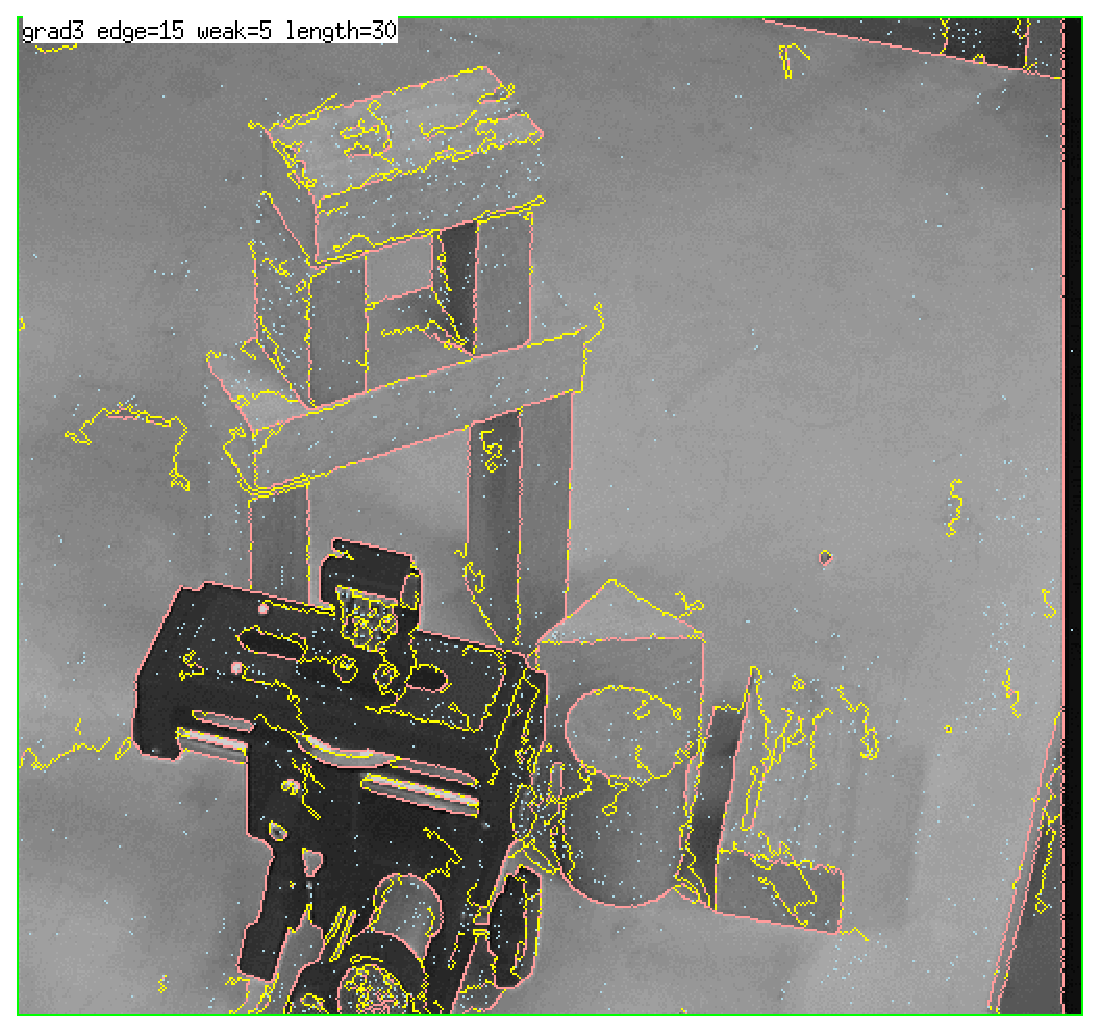
\includegraphics[height=9cm]{fig/block1.edg.ps}
%\epsfile{file=fig/block1.edg.ps,height=9cm}
\caption{Edge Finder and Overlaid Edges}
\end{center}
\end{figure}
\subsection{\label{tracking}Tracking}
{\tt "vision/correlation"} defines functions to find
correlation between window-image and tracking-image.

\begin{refdesc}
\classdesc{tracking-window}{pixel-image}{x-pos y-pos x-vel y-vel\\
\>pattern-size window-size\\
\>x-win y-win window window-margin\\
\>update threshold half-pattern correlation}{
This class defines tracking window.}

\methoddesc{:correlation}{}{
returns correlation between window-image and this image.}
\methoddesc{:grab}{\&optional (x x-pos) (y y-pos) (sampling 2)}{
grabs video image and returns grabbed pixel-image.}
\methoddesc{:window-rectangle}{val}{
draws rectangle on xwindow.}
\methoddesc{:rectangle}{val}{
draws rectangle on xwindow.}
\methoddesc{:move}{newpos \&aux (newx (aref newpos 0)) (newy (aref newpos 1))}{
moves tracking-window to {\em newpos} and grabs video image.}
\methoddesc{:track}{display-window \&optional th}{
tracks this image from window image.}
\methoddesc{:search}{display-window \&optional th}{
searches this image from window image.}
\methoddesc{:track-and-search}{flag \&optional th}{
tracks this image. If mistake tracking, searches this image from window image.}

\methoddesc{:pos}{}{
returns up-left position of window.}
\methoddesc{:vel}{}{
returns tracking velocity.}
\methoddesc{:insidep}{pos \&aux (x (aref pos 0)) (y (aref pos 1))}{
checks {\em pos} that is contained with tracking window.}
\methoddesc{:update}{\&optional (flag :get)}{
sets {\em flag} as update. if flag doesn't exist, returns update.}
\methoddesc{:prin1}{strm \&rest mesg}{
prints this tracking-window object with its name and dimensions.}
\methoddesc{:init}{x y size win-size}{
creates tracking-window object and sets slots.}
\end{refdesc}

\subsection{\label{PBMfile}Image File I/O}
%There are lots of file formats defined for the representation of
%pixel images.
{\tt "vision/pbmfile"} defines functions to transfer
image data between EusLisp and disk files.
EusLisp can read and write pgm
(portable gray-scale map) 
and ppm (portable pixmap) format files.

\begin{refdesc}
\funcdesc{read-pnm}{f \&optional buf0 buf1 buf2}{
reads a pgm or ppm file specified by file-stream {\em f} 
and returns a pixel-image or color-pixel-image object.
The image file can be either in ascii (P2 and P3) or in binary (P5 and P6) 
format.}
\funcdesc{read-pnm-file}{file \&optional buf0 buf1 buf2}{
reads a pgm or ppm file specified by filename {\em file}.}

\funcdesc{write-pgm}{f image  \&optional (depth 255)}{
writes a pixel-image specified by {\em image} into {\em f} file-stream
in the binary ppm format.
%(This function will be changed to allow adding comments.)
}
\funcdesc{write-ppm}{f image  \&optional (depth 255)}{
writes a pixel-image specified by {\em image} into {\em f} file-stream
in the binary pgm format.}
\funcdesc{write-pnm}{f img}{
writes a pixel-image specified by {\em img} into {\em f} file-stream.
If {\em img} is {\bf pixel-image}, it is written in the binary pgm format.
If {\em img} is {\bf color-pixel-image}, written in the binary
ppm format.}
\funcdesc{write-pnm-file}{file img}{
writes the pixel-image specified by {\em img} into {\em file}.
}
\funcdesc{image::read-raw-image}{file \&optional (x 256) (y x)}{
reads a raw-image file and returns a one-dimensional byte-vector (string).
%No assumption is made about the coordinates.
The dimensions of the raw-image must match with give {\em x} and {\em y}.
}
\funcdesc{image::write-raw-image}{file imgvec}{
writes pixel-values stored in a byte vector (string), {\em imgvec},
in {\em file}.}

\end{refdesc}


\subsection{JPEG compression/decompression}

EusLisp can link libjpeg.so in order to handle JPEG images.
Loading "eusjpeg.l" will define JPEG-compression and -decompression
functions.


\newpage
\section{\label{ManipulatorModel}Manipulators}
\markright{\arabic{section}. Manipulators}
\hfill {\em documented by Hiromu Onda}


Instances of {\bf rotational-joint} class and {\bf manipulator} class 
constitute a Manipulator Model. {\bf rotational-joint} is a subclass of the 
{\bf body}. {\bf manipulator} is a subclass of the {\bf cascaded-coords}.
{\bf rotational-joint} class defines models of manipulator joints. 
{\bf manipulator} class has methods for solving a forward kinematic solution and 
inverse kinematic solution. 

The way of the definition of a manipulator is that i) Make all the 
joints of the manipulator, ii) Integrate these joints into {\bf manipulator}.



\subsection{
Rotational Joint
%\label{JointModel}Rotational Joint
}

{\bf rotational-joint} describes a model of a joint. 
{\bf rotational-joint} has {\bf body} as super-class.
This class manages a model of shape, coordinates, rotation axis of a joint, 
angles of rotation, limits of joint angles, etc.
{\bf defjoint} macro below creates an instance of {\bf rotational-joint}.
This instance is bound to {\em joint-name}. Assign a ancestor joint to 
{\bf parent}. It is not necessary to assign rotational axes to base nor 
fingers. 

\ptext{
(defjoint \= {\it joint-name} \hspace{0.5cm} \=  \\ % \hspace{4cm} \=\\
\>        :shape \> {\it body-object} \\
\>        :color \> {\it color-id} \hspace{2cm} \= ;0-15 for MMD \\
\>        :parent \> {\it parent-joint} \\
\>        :axis \> {\it rotational-axis} \>  ; :x, :y or :z \\
\>        :offset \> {\it trans-from-parent-joint} \\
\>        :low-limit \> {\it joint-angle-limit-low} \\
\>	  :high-limit \> {\it joint-angle-limit-hight} \\
\>        ) \\}

\subsection{
Multi-Joint Manipulators
%\label{MultiJointsManipulator}Multi-Joint Manipulators
}

A model of a manipulator is described by {\bf manipulator}. 
{\bf defmanipulator} macro below creates an instance of {\bf manipulator}. 

\ptext{
(defmanipulator {\it manipulator-name} \\
\hspace{2cm} \= :class \hspace{2cm} \= {\it manipulator-class} \\
\> :base \> {\it base-joint} \\
\> :joints \>  {\it list-of-all-joints} \\
\> :hand \> {\it handjoint} \\
\> :left-finger \> {\it left-finger}\\
\> :right-finger \> {\it right-finger}\\
\> :handcoords \> {\it trans-from-hand-to-armsolcoords}\\
\> :toolcoords \> {\it trans-from-armsolcoords-to-toolcoords} \\
\> :open-direction \> {\it finger-open-direction}\\
\> :right-handed  \> {\it righty-or-lefty} \\
\>        ) \\
}
\begin{refdesc}	
\classdesc{rotational-joint}{body}{(axis offset high-limit low-limit)}{
describes each rotational joint of a 6 D.O.Fs manipulator.}
\classdesc{manipulator}{cascaded-coords}{(\= base baseinverse joint\\
\> angles right-handed hand handcoords right-finger left-finger\\
\>openvec max-span toolcoords toolinverse armsolcoords\\
\> toolinverse armsocoords approach grasp affix)}
{manages kinematics of a manipulator from base to hand.}
\methoddesc{:newcoords} {newrot \&optional newpos}{ 
updates the coords with newrot and newpos if new joint angles are within the 
limit.
}
 \methoddesc{:armsolcoords } {}{
computes and makes transformation (an instance coords) 
between the coords of the 
base and those of the hand. 
}
 \methoddesc{:tool} {\&rest msg}{
modifies or gets toolcoords.
}
 \methoddesc{:set-tool} {newtool \&optional offset copy}{
sets new toolcoords.
}
 \methoddesc{:reset-tool } {}{
forces this coords to be default-toolcoords.
}
 \methoddesc{:worldcoords } {}{
computes the position vector, the rotation matrix, and the coordinates of the 
toolcoords represented in the world coordinates. 
}
 \methoddesc{:set-coords } {}{
forces setting coords according to the forward kinematic solution.
}
 \methoddesc{:config } {\&optional (a newangles)}{
sets joint angles of the manipulator.
}
 \methoddesc{:park } {}{
forces all the joint angles to be zero.
% 初期姿勢に戻す
}
\methoddesc{:hand}{\&optional (h nil)}{
sets or returns the object of its hand.
%  ハンドオブジェクトを返す
}
\methoddesc{:handcoords}{}{
computes the position vector, the rotation matrix, and the coordinates of the 
handcoords represented in the world coordinates. 
% ハンド座標系ののワールド表現を求める
}
\methoddesc{:span}{}{
returns the current distance between fingers.
%  現在の指の間隔を返す
}
\methoddesc{:open-fingers}{s \&optional abs \&aux (current (send self :span))}
{moves fingers relatively or absolutely.
% 指幅を相対的、絶対的に指定する
}
\methoddesc{:close-fingers} {}{
closes fingers completely.
% 指を完全に閉じる 
}
\methoddesc{:angles} {\&optional flag}{
returns the list of current joint angles.
% 現在の姿勢の関節角度のリストを返す
}
% \methoddesc{:right-handed} {}{
%% ソースそのものがありませんでした。
% 右手姿勢、左手姿勢を選択する
%}
 \methoddesc{:get-approach } {}{
returns the object to which the hand is approaching.
% 現在アプローチしている対象を返す
}
 \methoddesc{:set-approach } {a}{
sets {\it a} as the object to which the hand will approach.
% アプローチ対象を設定する
}
 \methoddesc{:get-grasp} {}{
(:get-grasp () grasp-config)
%??? 
% 把握姿勢にある対象物を返す
}
 \methoddesc{:set-grasp} {g}{
sets {\it g} as the object which the hand will grasp.
% 把握対象物を指定する
}
 \methoddesc{:get-affix} {}{
returns the object which the hand grasps.
% 把握している物体を返す
}
 \methoddesc{:affix} {\&optional (grasp)}{
sets {\bf affixed-object} {\bf grasp}.
{\bf grasp} is associated to the handcoords as a descendant. 
% 把握を指示する
}
 \methoddesc{:unfix} {\&optional (margin 10.0)}{
sets {\bf affixed-object} nil.
{\bf grasp} is dissociated (removed) from the descendants list of the handcoords.
% 把握物体を解放したことを指示する
}
\longdescription{:create}{\=\&rest args \`[method]\\
           \>\&key \=((:name nm)) ((:hand h)) ((:joints j))
                ((:left-finger lf)) ((:right-finger rf))\\
               \>\> ((:toolcoords tc) (make-coords))
                ((:handcoords hc) (make-coords))\\
                \>\>((:base bs) (make-cascoords))
                (open-direction (floatvector 0 1 0))\\
                \>\>((:max-span mspan) 100.0)
                ((:lefty lft) t)
                ((:act a) nil)\\
            \>\&allow-other-keys}{
creates and initializes a new manipulator object.
% 新しいマニピュレータオブジェクトを作成、初期化する
}

\end{refdesc}
{\bf manipulator} manages the linkage of the coords of 
{\bf base, joints(J1\ldots J6), handcoords, toolcoords}. 
{\bf manipulator} has {\bf cascaded-coords} as super-class. 
{\bf manipulator} is connected with {\bf base} which is {\bf cascaded-coords}
(or subclasses of {\bf body}). {\bf manipulator} manages the transformation from 
the base frame to the toolcoords. Messages sent to {\bf manipulator} 
(i.e. {\bf :translate, :locate, :rotate, :orient, :transform} etc.) effect 
the end effector of the manipulator. If WRT parameter is set one of keywords 
(i.e. :local, :parent, :world or an instance of coordinates) in this message, 
the end-effector  moves with respect to the WRT parameter. 
In the next program {\bf eta3} is a instance of {\bf manipulator}.

%{\bf manipulator}オブジェクトは、
%{\bf base、joints(J1\ldots J6)、handcoords、toolcoords}
%の座標系の連鎖を管理する。
%図\ref{ManipulatorObject}に{\bf manipulator}オブジェクトのスロット構成を、
%表\ref{ManipulatorMethods}に受け付けられるメソッドを掲げる。
%{\bf manipulator}クラスは、{\bf cascaded-coords}のサブクラスであり、
%やはり、{\bf cascaded-coords}(または{\bf body}などのサブクラス)
%である{\bf base}に結合され、
%{\bf base}から{\bf toolcoords}(手先座標系)への変換を管理している。
%したがって、{\bf manipulator}オブジェクトに対して送られる
%{\bf :translate、:locate、:rotate、:orient、:transform}
%などのメッセージは、手先点に対して作用する。
%そのとき同時にWRTパラメータを指定すれば、
%手先はWRT座標系に対して動く。
%次のプログラムでは、{\bf eta3}を{\bf manipulator}のインスタンスと仮定している。


\begin{verbatim}
 (send eta3 :translate #f(0 0 -100))        ;put back the end-effector by 10cm
 (send eta3 :translate #f(0 0 -100) :world) ;move down the end-effector by 10cm
 (send eta3 :translate #f(0 0 -100)
             (manipulator-base eta3))  ;move down the end-effector with respect 
                                       ;to the coords of the base by 10cm
\end{verbatim}

%\begin{verbatim}
% (send eta3 :translate #f(0 0 -100))        ;手先を10cm引っ込める 
% (send eta3 :translate #f(0 0 -100) :world) ;10cm下げる
% (send eta3 :translate #f(0 0 -100)
%             (manipulator-base eta3))     ;手先をベース座標系で10cm下げる
%\end{verbatim}

When {\bf manipulator} receives these messages, it calculates the arm solution 
and 6 joint angles are determined. Generally, more solutions than one exist.
In that case, one appropriate solution is chosen of them according to the 
criteria (i.e. the distinction between {\bf right-handed} and {\bf left-handed},
and the consistency with current joint angles). If there is no solution for 
a given configuration or the calculated joint angles exceed its limits, 
{\bf manipulator} does not move and it gives a warning.

%これらのメッセージに対して、manipulatorはアーム解を計算して6つの
%関節角度を決定する。
%一般に解は複数存在するが、{\bf right-handed}(右手系、左手系)
%の区別、および現在の関節角度との連続性により適当な解が選択される。
%しかし、指定された位置、姿勢に対する解が存在しない場合や関節角が
%限界を越える場合は移動、回転は起こらず、警告が発せられる。

Arm-solution method {\bf :armsol} must be defined for respective manipulator 
classes which correspond to real manipulators. This method calculates the 
transformation between the base-coords and the hand-coords. Thus this allow us 
to put a manipulator wherever with respect to the world-coords. The arm solution 
is independent of the {\bf base, toolcoords}.

%アーム解の計算は、実際のマニピュレータに対応した
%個々のmanipulatorクラスに定義された{\bf :armsol}メソッドが行う。
%マニピュレータがワールド座標系のどこに置かれてもよいように、
%また、どのような工具を用いてもよいように、アーム解は、
%{\bf base、toolcoords}とは独立に、base座標系中でのハンドの位置、姿勢に
%対して与えられる。

Fig. \ref{JointCoords} shows the relation between coordinate systems 
({\bf base, J1, J2,\ldots , handcoords} and {\bf toolcoords}). $T$ and other 
transformations are calculated as follows.

%{\bf base、J1、J2、\ldots 、handcoords、toolcoords}の関係を図\ref{JointCoords}
%に示す。
%ワールドから手先への変換を$T$とすると、$T$および各部分変換は次のようにし
%て得られる。

$
\begin{array}{ll}
T & = base \cdot J1 \cdot J2 \cdot \ldots 
\cdot J6 \cdot handcoords \cdot toolcoords \\ 
 & = (send \; eta3 \; :worldcoords) \\ 
T_{Jn} & = base \cdot J1\cdot \ldots \cdot Jn \\
 & = (send \; Jn \; :worldcoords) \\
T_{arm} & = J1 \cdot J2 \cdot \ldots \cdot J6 \cdot handcoords \\ 
 & = (send \; eta3 \; :armsol-coords) \\ 
T_{tool} & = J1 \cdot J2 \cdot  \ldots \cdot J6 \cdot handcoords \cdot toolcoords \\ 
 & = (send \; eta3 \; :copy-coords) \\
T_{t} & = toolcoords \\ 
 & = (manipulator-toolcoords \; eta3)\\
T_{t}^{-1} & = toolcoords^{-1} \\ 
 & = (manipulator-toolinverse \; eta3) \\
T_{h} & = handcoords \\ 
 & = (manipulator-handcoords \; eta3)\\
\end{array}$

where $T$ is the transformation between the world-coords and the toolcoords.

\begin{figure}
\begin{center}
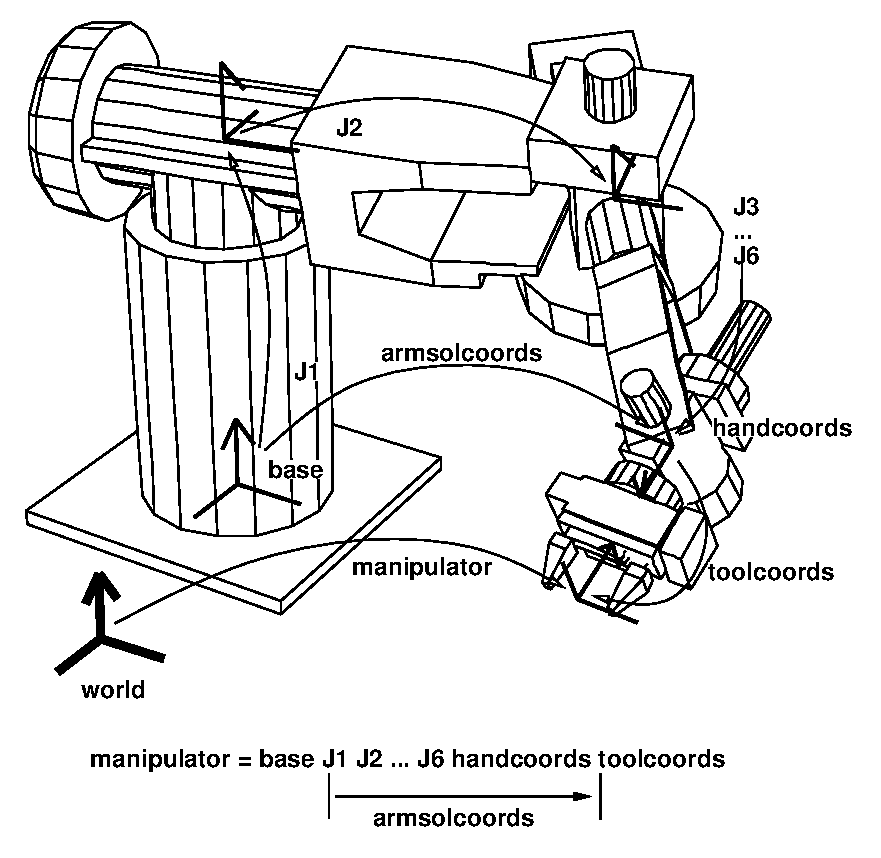
\includegraphics[height=100mm]{fig/eta3coords.ps}
%\epsfile{file=fig/eta3coords.ps,height=100mm}
%\mbox{
%\epsfysize=10cm
%\epsfbox{fig/eta3coords.ps}
%}
\end{center}
\caption{\label{JointCoords}
relation between coordinate systems in a manipulator}

\end{figure}

Each joint has a geometric model represented by Breps (Boundary Representation).
The coordinates of the vertices and the equations of the planes are not always 
current ones. Messages sent to {\bf manipulator} for translation or rotation only
update the coordinate systems, these do not update the coordinates of the 
vertices. This is why we can reduce the calculation time when translation or 
rotation occurs successively. If {\bf :worldcoords} message is sent to 
{\bf manipulator}, it updates the data such as the coordinates of the vertices.

%各関節は、Brepで表現された幾何モデルを保持している。しかし、頂点の座標、
%平面の方程式は常に現状を反映しているとは限らない。マニピュレータに対する
%移動、回転などのメッセージでは座標系の更新だけを行い、頂点の座標は変化し
%ない。これは、移動、回転が複数回続けて起こった場合の計算量を減らすためで
%ある。更新は、マニピュレータに{\bf :worldcoords}メッセージを送る
%ことで引き起こされる。

Mainly toolcoords are used for specify the motion of a manipulator in 
this {\bf manipulator}. There is a method ({\bf :config}) for specifying the 
configuration of the manipulator by joint angles. The arguments are a 
float-vector whose elements are 6.

%マニピュレータは、手先座標系で動作を指定することを主な目的としている。
%関節角による指定には {\bf :config} を用いる。
%引き数には6要素の列を与える。

\begin{verbatim}
  (send eta3 :config (float-vector pi/2 pi/2 0 1 0 1))
\end{verbatim}

{\bf :config} rotates joints of the manipulator if the joint angles are in the 
limit. As a result, the coordinates which {\bf manipulator} manages and the 
current toolcoords which given joint angles determines become inconsistent.
{\bf :set-coords} message must be sent if you need consistency. {\bf :set-coords}
calculates a forward kinematic solution and calculates the arm solution using the 
forward kinematic solution.


%{\bf :config}は、各関節角度が可動範囲に収まっていることを検査した後、
%それらを回転させる。
%この結果、マニピュレータの管理している座標系と
%関節角度から定まる実際の手先の位置姿勢とが一致しなくなる。
%両者を一致させるためには、{\bf :set-coords}メッセージを送る。
%{\bf :set-coords}は、関節角度から順方向のキネマティクスを計算し、
%最終的な手先座標系に対してさらにアーム解を解く。

Example: create the manipulator model (ETA3) and draw this on a Xwindow system.
\begin{verbatim}
;EusLisp 7.27 with Xlib created on Thu Sep 17 14:33:30 1992
(load "view.l")                                ;open a window
(load "/usr/local/eus/robot/eta3/eta3build.l") ;create the model of ETA3
(send *viewing* :look #f(2000 2000 2000))      ;change the viewpoint
(send-all (eta3arm-components eta3) :color 1)  ;change the color of lines
(send eta3 :config (float-vector 0 (/ -Pi 4.0) Pi/2 0 (/ -Pi 4.0) 0 ))
					       ;set joint angles of ETA3
(send eta3 :set-coords)                        ;refer to the above explanation
(draw eta3)                                    ;draw ETA3
\end{verbatim}


%例 ETA3のモデル生成とその描画
%\begin{verbatim}
%EusLisp 7.27 with Xlib created on Thu Sep 17 14:33:30 1992
%(load "view.l")                                ;ウィンドウを開く
%(load "/usr/local/eus/robot/eta3/eta3build.l") ;ETA3のモデルを生成する
%(send *viewing* :look #f(2000 2000 2000))      ;視点を変える
%(send-all (eta3arm-components eta3) :color 1)  ;物体の線の色を黒に変える
%(send eta3 :config (float-vector 0 (/ -Pi 4.0) Pi/2 0 (/ -Pi 4.0) 0 ))
%					       ;ETA3を関節角度の指定で動かす
%(send eta3 :set-coords)                        ;上記参照
%(draw eta3)                                    ;ETA3を描画する
%\end{verbatim}

\clearpage

% \newpage

\section{\label{MARS} MARS: A Multiple Autonomous Robot Simulator}
\markright{\arabic{section}. MARS}
\hfill {\Large \em (Preliminary Announcement)}

\hfill {\em Author: Yasuo KUNIYOSHI, ETL}

{\bf MARS} is a graphical simulation environment for multiple autonomous
mobile robots in 2D space.  This program is written in EusLisp.

{\bf Development Status:} As of Janurary, 1995, a pre-release version
of MARS is in use within ETL. We are actively improving the system and
plan to release the first version within the first half of 1995. We
will continue enhancing the system thereafter and hopefully achieve a
stable state by March 1996. Release announcements will be made through
the euslisp mailing list and other internet services.
Possibly we will adopt licencing conditions separate from the EusLisp.

{\bf Purpose:}
MARS is intended for use in intelligent robotics research on
single/multiple mobile robot(s), such as behaviour learning, map
building, collective intelligence, multi-robot cooperation,
cooperative learning, etc.


\subsection{How to Start} The MARS program resides in {\bf
robot/MARS/ver.XXX}. First, copy the ".eursrc" file to your home
directory. Make necessary changes. (Pathname of the directory in which
MARS is installed.)

Invoke {\bf eusx} in this directory,  and all the files are
automatically loaded and the simulator starts running.
Wait until a window opens and an initial message appears in the bottom window.

Example:
\begin{verbatim}
Try "SYSTEM"->"Load" menu.
Load "example.bbs".
And "SCL"->"On" menu.
\end{verbatim}

Notes:\\
SCL$\rightarrow$"Off" Pauses the simulation but continue GUI processing.\\
SYSTEM$\rightarrow$"Quit" Exits the toplevel loop. Can be resumed by (mars-loop).\\
SYSTEM$\rightarrow$"Save" Saves the current state to a file.\\
SYSTEM$\rightarrow$"All-Clear" Clears everything and initializes the system.\\
SYSTEM$\rightarrow$"Reset" Is used to reset internal states of the robots
(Special purpose).\\

\subsection{System Overview}

\begin{figure}[h]
\begin{center}
%\begin{tabular}{c@\extracolsep{1em}c}
\begin{tabular}{c c}
%\epsfile{file=fig/mars.eps,scale=0.3} & % ɽ���Ʊ�������ѹ����ơ�
\mbox{
\epsfsize=10cm
\epsfbox{file=fig/mars.eps}
}
%\epsfile{file=fig/simst.ps,hscale=0.42,vscale=0.45} \\
\mbox{
\epsfsize=10cm
\epsfbox{file=fig/simst.ps}
}
\end{tabular}
\caption{\label{MARSOverview} MARS window display example (left).
And overall program structure (right).}
\end{center}
\end{figure}

When you start up MARS, you will see the main window as shown in
Fig.~\ref{MARSOverview}(left). The MARS system adopts a modular
architecture as in Fig.~\ref{MARSOverview}(right). It consists of
a physcial simulation module, robot control modules, a graphical user
interface module (GUI), and a user defined global control loop.

{\bf Physical Simulation:}
Our current physical simulation module handles four types of objects,
{\bf wall} (static obstacles), {\bf block} (passive objects), {\bf
robot-body} (active objects), and {\bf magic-block} (special
reward-giving objects for learning experiments).

\begin{figure}
\begin{center}
%\begin{tabular}{c@\extracolsep{1em}c}
\begin{tabular}{c c}
%\epsfile{file=fig/robot-ui2.ps,hscale=0.5,vscale=0.5} &
\mbox{
\epsfsize=10cm
\epsfbox{file=fig/robot-ui2.ps}
}
%\epsfile{file=fig/robot-st2.ps,scale=0.4} \\
\mbox{
\epsfsize=10cm
\epsfbox{file=fig/robot-st2.ps}
}
\end{tabular}
\end{center}
\caption{\label{fig:robotst} Internal structure of a robot object
(left). And an example behavior-based robot configuration (right).}
\end{figure}

{\bf Robot Models:}
There is a clear interface between the physical simulation module and
robot control modules. Any number of {\bf robot} models can be
generated and simulated in (pseudo-)parallel.
Each {\bf robot} consists of a pair of modules,
a {\bf robot-body} and a {\bf robot-brain}.
A {\bf robot-body} defines physical properties of a robot and a {\bf
robot-brain} defines how the robot behaves.

{\bf Sensor Models:}
A user can choose and attach any number of sensors to any place of a
{\bf robot-body}. Currently available sensor models are as follows:
{\bf distance} (odometry), {\bf angle} (rotation), {\bf touch}, {\bf
infrared}, {\bf radar} (sonar), {\bf eye} (object-name-sensor).
Noise or uncertainty is not considered in the current version.

{\bf Robot Brains:}
A {\bf robot-brain} is a user defined module for processing the
simulated sensor data and generating action commands.
It must accept sensor data and output action commands. In addition, it
must be written as a re-entrant program, time-sliced by a {\bf :step}
message sent by the global control loop.
As long as these constraints are met, a user can adopt any cognitive
architecture. The system provides an example behavior-based type
architecture as a default.

{\bf GUI:}
The {\bf MARS} main window has a menu-bar with several buttons for
controlling the system. Also, the system has a built-in graphical
editor for creating/modifying the physical environment.
You can save/load a physical environment definition together with
agent definitions to/from a file.

{\bf Network Extension:}
A {\bf robot-brain} can be configured to be connected to external
process via an asychronous socket connection. In this case, a user can
use an arbitrary language (C, Prolog, Scheme, Perl, etc...) to write
the {\bf remote-brain}. Thanks to the asynchronous connection, a user
do not have to mind about time slicing at all.

{\bf Facility for Learning Experiments:}
{\bf MARS} provides several special functionalities for robot learning
experiments: reward-giving objects, reward sensors (send reward values
to each robot), and a reward-logger (accumulates a system-wide reward
statistics.)


\markboth{EusLisp version \eusversion Reference Manual (Part IV)}{X-windows}
\section{Xwindow Interface}
\markright{\arabic{section}. Xwindow}
The Xwindow interface on EusLisp becomes available when EusLisp is
invoked by the name of {\tt 'eusx'}.
\footnote{Eusx is a symbolic link to eus.}
The "DISPLAY" environment variable should be properly set to your Xserver,
since eusx tries to connect to Xserver referencing
the "DISPLAY" environment variable when it starts up.

EusLisp defines three levels of xwindow interface:
(1) Xlib functions, (2) Xlib classes, and (3) XToolKit classes.
All the xwindow functions described in this section and the following
XToolKit section are contained in the "X" package.
The function names of the original Xlib are changed so that
all constituent letters are converted to upcase
and the first 'X' prefix is removed.
For example, {\tt XdefaultGC} is named {\tt X:DEFAULTGC},
not {\tt X:XDEFAULTGC}.

The Xlib functions are defined as foreign functions
as the lowest level interface to Xwindow system.
These Xlib functions should be used carefully, 
since parameter type check or parameter number check is not performed.
For an instance, all the Xlib call requests {\tt x:*display*} argument
to identify the connection to Xserver, and if you forget it, Xlib reports
an error and the process dies.
The second level interface, Xlib classes are provided
to avoid this inconvenience and to make the interface object-oriented.
%By instantiating the xwindow class, you will get a window on a screen,
%and sending messages to the instance, you can draw lines, strings, or whatever
%in it.
This section focuses on this second level interface.
Even higher level xwindow library called XToolKit is explained 
in the next section.

Classes described in this section have the following inheritance
hierarchy.

\begin{quote}
\begin{verbatim}
propertied-object
   viewsurface
      x:xobject
         x:gcontext
         x:xdrawable
             x:xpixmap
             x:xwindow
   colormap
\end{verbatim}
\end{quote}

\subsection{\label{xvariables}Xlib global variables and misc functions}
\begin{refdesc}
\vardesc{x:*display*}{X's display ID (integer).}
\vardesc{x:*root*}{default root window object. }
\vardesc{x:*screen*}{default screen ID (integer).}
\vardesc{x:*visual*}{default visual ID (integer).}
\vardesc{x:*blackpixel*}{black pixel = 1}
\vardesc{x:*whitepixel*}{white pixel = 0}
\vardesc{x:*fg-pixel*}{default foreground pixel referenced at window creation,
normally {\tt *blackpixel*}.}
\vardesc{x:*bg-pixel*}{background pixel referenced at window creation,
normally {\tt *whitepixel*}}
\vardesc{x:*color-map*}{the system's default color-map}
\vardesc{x:*defaultGC*}{the default gcontext referenced at pixmap creation.}
\vardesc{x:*whitegc*}{GC whose foreground color is white.}
\vardesc{x:*blackgc*}{GC whose foreground color is black.}

% \vardesc{*gray-gc*}{half-tone GC}
\vardesc{*gray-pixmap*}{the result of {\tt (make-gray-pixmap 0.5)}}
\vardesc{*gray25-pixmap*}{16x16 pixmap,
a quarter of pixels are {\tt *fg-pixel*} and three quarters {\tt *bg-pixel*}.}
\vardesc{*gray50-pixmap*}{16x16 pixmap, a half of pixels are {\tt *fg-pixel*}.}
\vardesc{*gray75-pixmap*}{16x16 pixmap, three quarters of pixels are black.}
\vardesc{*gray25-gc*}{25\% gray GC made from  {\tt *gray25-pixmap*}.}
\vardesc{*gray50-gc*}{50\% gray GC made from  {\tt *gray50-pixmap*}.}
\vardesc{*gray75-gc*}{75\% gray GC made from  {\tt *gray75-pixmap*}.}
\vardesc{*gray*}{{\tt "\#b0b0b0"}}
\vardesc{*bisque1*}{{\tt "\#ffe4c4"}}
\vardesc{*bisque2*}{{\tt "\#eed5b7"}}
\vardesc{*bisque3*}{{\tt "\#cdb79e"}}
\vardesc{*lightblue2*}{{\tt "\#b2dfee"}}
\vardesc{*lightpink1*}{{\tt "\#ffaeb9"}}
\vardesc{*maroon*}{{\tt "\#b03060"}}
\vardesc{*max-intensity*}{65535}
\vardesc{font-cour8}{{\tt (font-id "*-courier-medium-r-*-8-*")}}
\vardesc{font-cour10}{{\tt (font-id "*-courier-medium-r-*-10-*")}}
\vardesc{font-cour12}{{\tt (font-id "*-courier-medium-r-*-12-*")}}
\vardesc{font-cour14}{{\tt (font-id "*-courier-medium-r-*-14-*")}}
\vardesc{font-cour18}{{\tt (font-id "*-courier-medium-r-*-18-*")}}
\vardesc{font-courb12}{{\tt (font-id "*-courier-bold-r-*-12-*")}}
\vardesc{font-courb14}{{\tt (font-id "*-courier-bold-r-*-14-*")}}
\vardesc{font-courb18}{{\tt (font-id "*-courier-bold-r-*-18-*")}}
\vardesc{font-helvetica-12}{{\tt (font-id "*-Helvetica-Medium-R-Normal-*-12-*")}}
\vardesc{font-lucidasans-bold-12}{{\tt (font-id "lucidasans-bold-12")}}
\vardesc{font-lucidasans-bold-14}{{\tt (font-id "lucidasans-bold-14")}}
\vardesc{font-helvetica-bold-12}{{\tt (font-id "*-Helvetica-Bold-R-Normal-*-12-*")}}
\vardesc{font-a14}{{\tt (font-id "*-fixed-medium-r-normal-*-14-*")}}

%\vardesc{x:*reversevideo*}{}
\vardesc{x:*xwindows*}{a list of all windows including subwindows
created and maintained by EusLisp.}
\vardesc{x:*xwindow-hash-tab*}{a hash table to look up the xwindow object
by its drawable ID.
In the event structure obtained by {\tt x:nextevent} is a window ID,
and {\tt x:window-main-loop} calls {\tt x:event-window} to know
the corresponding xwindow object using this table.}
%\vardesc{x:gcval}{}

\funcdesc{xflush}{}{
sends all commands retained in the Xlib command buffer to Xserver.
Since Xlib buffers output to Xserver,
commands you issued commands to Xserver are not executed immediately.
This is necessary to decrease network traffic and the frequency
of process switching.
To flush the command buffer to see the effects of the commands,
use {\bf xflush} or send {\bf :flush}
message to  xwindow objects.
}
\funcdesc{find-xwindow}{subname}{
Each xwindow may have name specified at the creation time.
Find-xwindow looks in the *xwindows* list and returns a list
of windows that have 'subname' as a substring
of its name. }

\end{refdesc}

\subsection{Xwindow}

\begin{refdesc}

\classdesc{Xobject}{geometry:viewsurface}{}{
The common super class for all the Xwindow related classes.
Currently, no slots variables and methods are defined.}

\classdesc{Xdrawable}{Xobject}
{(drawable  \hspace{10mm} \=  ; drawable  ID \\
 \> gcon \>  ; this drawable's default graphic context object\\
\> bg-color \> ; background color \\
\> width height \> ; horizontal and vertical dimensions in dots}
{{\bf Xdrawable} defines rectangular regions where graphics objects such as
lines and strings can be drawn.
{\bf Xdrawable} is an abstract class to define
common methods for xwindow and xpixmap,
and instantiation of this class has no effect.}

\methoddesc{:init}{id}{
{\em Id} is set to the {\em drawable} slot as the ID of this drawable.
A new GC (graphic context) is created and set to {\em gcon} as 
the default GC of this drawable object.}
\methoddesc{:drawable}{}{returns drawable id.}
\methoddesc{:flush}{}{flushes commands retained in the Xlib's buffer.}
\methoddesc{:geometry}{}{
returns the list of seven geometric attributes,
{\em root-window-id, x-position, y-position,
width, height, border-width} and {\em visual's depth}.}
\methoddesc{:height}{}{
returns the height (dots in y direction) of this drawable.}
\methoddesc{:width}{}{
returns width (dots in x direction) of this drawable.}
\methoddesc{:gc}{\&rest newgc}{
If no {\em newgc} is given, the current gc object is returned.
If {\em newgc} is an instance of gcontext,
it is set to the gc of this drawable.
Otherwise, {\em newgc} is regarded as a message and  sent to
the current gc.}
\methoddesc{:pos}{}{returns an integer vector representing 
the position of this drawable.
The position is always defined relative to the 
parent window, and windows created as direct subwindows of the root
window under the intervention of the window manager return the constant
coordinates in their surrounding title window regardless to their
true position in the root.}
\methoddesc{:x}{}{returns the {\em x} coordinate of this drawable relatively to
the parent window.}
\methoddesc{:y}{}{returns the {\em y} coordinate of this drawable relatively to
the parent window.}

\methoddesc{:copy-from}{drw}{
{\em Drw} is another drawable object (xwindow or pixmap).
The contents of {\em drw} is copied to this drawable.}

\begin{figure}
\begin{center}
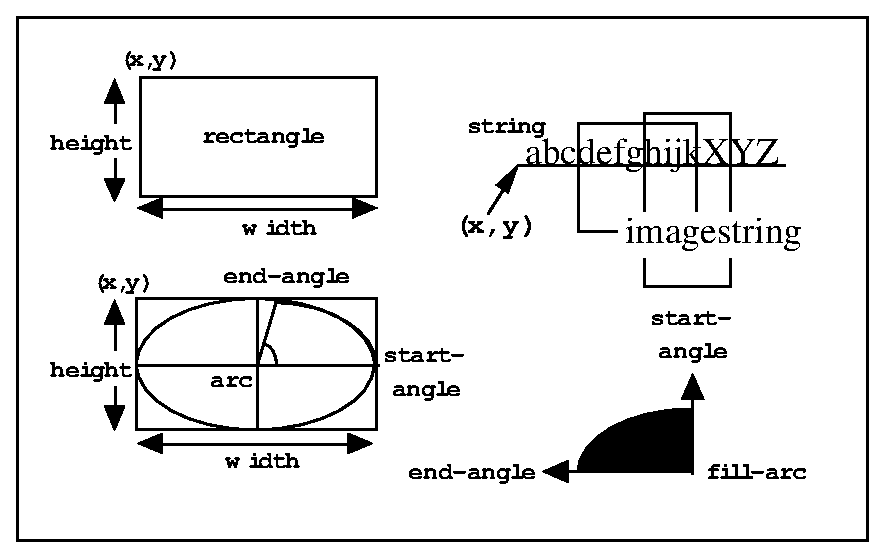
\includegraphics[height=6cm]{fig/xdraw.ps}
%\epsfile{file=fig/xdraw.ps,height=6cm}
%\mbox{
%\epsfysize=6cm
%\epsfbox{fig/xdraw.ps}
%}
\end{center}
\caption{drawing primitives\label{xdraw}}
\end{figure}


\methoddesc{:point}{x y \&optional (gc gccon)}{
draws a point at $(x, y)$ with optional {\em gc}.}
\methoddesc{:line}{x1 y1 x2 y2 \&optional (gc gcon)}{
draw a line from {\em (x1, y1)} to {\em (x2, y2)}
with optional {\em gc}. {\em x1, y1, x2,} and{\em y2} must be integers.}
\methoddesc{:rectangle}{x y width height \&optional (gc gcon)}{
draws a rectangle whose center is located at {\em (x, y)}
and size is specified by {\em width} and {\em height}.}
\methoddesc{:arc}{x y width height angle1 angle2 \&optional (gc gcon)}{
draws an elliptic arc whose center is {\em (x, y)} and starting angle at 
{\em angle1} and ending angle at {\em angle2}.
Angles should be given by radian.}
\methoddesc{:fill-rectangle}{x y width height \&optional (gc gcon)}{
fills in a rectangular region.}

\methoddesc{:fill-arc}{x y width height angle1 angle2 \&optional (gc gcon)}{
fills in an arc.
}
\methoddesc{:string}{x y str \&optional (gc gcon)}{
displays the string {\em str} starting at {\em (x, y)}. The background is
not filled.}
\methoddesc{:image-string}{x y str \&optional (gc gcon)}{
displays an imagestring of {\em str}. Imagestring fills background.}
\methoddesc{:getimage}{\&key x y width height (mask \#ffffffff) (format 2)}{
gets ximage from the server and returns the pixel data in a string.
The pixel data sent from the server is once stored in Xlib's ximage structure,
then copied to the string row by row.
The ximage structure is automatically destroyed.
The image string obtained by {\tt :getimage} can be used to make
a {\tt pixel-image}, which can be written to a file in the pbm formats
as described in section \ref{PBMfile}.}
\methoddesc{:putimage}{image \&key src-x src-y dst-x dst-y width height ((:gc g) gc)}{
puts {\em image} to the specified location in this drawable.
{\em image} is a string or a address pointing to an ximage structure.}
\methoddesc{:draw-line}{from to}{
is same as {\bf :line} method,
and provided for the compatibility with other viewsurface classes.}
\methoddesc{:line-width}{\&optional dots}{sets line-width of this drawable's
default GC. Use of the {\tt :gc :line-width} message is recommended.}
\methoddesc{:line-style}{\&optional dash}{sets line-style of this drawable's
default GC. Use of the {\tt :gc :line-style} is preferable.}
\methoddesc{:color}{\&optional c}{sets color of this drawable.}
%\methoddesc{:set-show-mode}{}{
%sets copy mode. this function usually uses for monochrome display.}
%\methoddesc{:set-erase-mode}{}{
%sets erase mode. this function usually uses for monochrome display.}
%\methoddesc{:set-xor-mode}{}{
%sets xor mode. this function usually uses for monochrome display.}
\methoddesc{:clear}{}{
clears full screen. this method calls {\tt :clear-area}}
\methoddesc{:clear-area}{\&key :x  :y :width :height :gc}{
clears a rectangle using the {\tt :fill-rectangle} method.}

\classdesc{Xpixmap}{Xdrawable}{}{Pixmap is a drawable that is often used
as a picture buffer or a background pattern.
Unlike xwindow, pixmap itself is not visible until it is copied to xwindow
or pixmap does not generate any event.}

\methoddesc{:init}{id}{initializes this pixmap.}
\methoddesc{:create}{\&key (width 500) (height 500) (depth 1) (gc *defaultgc*)}{
creates a {\em width} x {\em height} pixmap with {\em gc} as its
default GC.}
\methoddesc{:create-from-bitmap-file}{fname}{
creates a pixmap from a bitmap file.}
\methoddesc{:write-to-bitmap-file}{fname}{
writes the contents of this pixmap into a bitmap file,
which can be read back to create a pixmap by {\bf :create-from-bitmap-file}
method.}
\methoddesc{:destroy}{}{
destroys this pixmap and frees X resources.}

%%%%%% X W I N D O W
\classdesc{Xwindow}{Xdrawable}{(parent subwindows backing-pixmap event-forward)
}{{\bf Xwindow} defines visible rectangular regions of the screen.
It is inherited not only by {\bfx text-window} and {\bf canvas} where
any graphics objects can be drawn, but also by many {\bf panel-items}
and {\bf scroll-bars}, which look like graphics objects rather than windows.}

\longdescription{:create}{\&key ( \= (:parent *root*) \` [method] \\
\> (x 0) (y 0) (size 256) (width size) (height size) (border-width 2) \\
\> (save-under nil) (backing-store :always) (backing-pixmap nil)\\
\> (border *fg-pixel*) (background *bg-pixel*) \\
\> (map T) (gravity :northwest) \\
\> (title "WINDOW") (name title) \\
\> (font) \\
\> event-mask (:key :button :enterLeave :configure :motion)}
{creates and initializes a xwindow.
When {\em parent} is given, this window is created as a subwindow
of {\em parent}, and is registered in the {\em subwindows} list of
the {\em parent}.
{\em X, y, size, width, height} and {\em border-width} determine
the location and the dimensions of this window.
{\em Save-under} and {\em backing-store} control the Xserver's behaviors
taken upon when the window is re-mapped. {\em Save-under} is either
T or NIL, while {\em backing-store} is either {\tt :notUseful, :WhenMapped},
or {\em :Always}.
When {\em backing-pixmap} is T, a pixmap of the same size as this window
is created by EusLisp, and maintained as a backing-store in case
the Xserver does not have the capability of backing-store.
{\em Border} and {\em background} specify the {\em border\_pixel}
and {\em background\_pixel} attributes, respectively.
{\em Map} should be set NIL, if this window should not appear
immediately after its creation, as is the case many small windows 
are created as panel-buttons in a {\bf panel}.
{\em Title} is the window title which appears in the title bar of 
the window.
{\em Name} is the name of the window stored in the property-list
of this xwindow object and printed by the printer.
X's events reported to this window are determined by 
{\em Event-mask}, that is, either an integer representing a bit-coded event-mask
or a list of the following symbols:
{\tt :key, :button, :enterLeave, :motion} and {\tt :configure}.
If more precise control is needed, the following symbols for each event
can be specified: {\em :keyPress, :keyRelease, :ButtonPress, :ButtonRelease,
:EnterWindow, :LeaveWindow, :PointerMotion, :PointerMotionHint, 
:ButtonMotion, :KeyMapState, :Exposure, :VisibilityChange, :StructureNotify,
:ResezeRedirect, :SubstructureNotify, :SubstructureRedirect,
:FocusChange, :PropertyChange, :ColormapChange} and {\tt :OwnerGrabButton}.
{\tt :Key} enables both {\tt :keyPress} and {\tt :KeyRelease}, and
{\tt :button} enables both {\tt :ButtonPress} and {\tt :ButtonRelease}.
When an event is sent from the server, {\bfx window-main-loop} analyzes
the event structure and send the {\tt :KeyPress, :KeyRelease, :buttonPress,
:ButtonRelease, :EnterNotify, :LeaveNotify, :MotionNotify, :ConfigureNotify}
message to the window where the event occurred.}

\methoddesc{:map}{}{makes this xwindow and all the subwindows visible.}
\methoddesc{:unmap}{}{makes this xwindow and all the subwindows invisible.}
\methoddesc{:selectinput}{event-mask}{
{\em Event-mask} is either an integer or a list of eventmask symbols.
Each event corresponding to the bit turned-on or 
enumerated in the {\em event-mask} list
becomes to be reported to this window.}
\methoddesc{:destroy}{}{destroys this xwindow and frees X resource.
The corresponding entries in {\tt *xwindows*} and {\tt *xwindow-hash-tab*}
are also deleted so that this window object could be garbage-collected.
All subwindows are also deleted by sending {\tt :destroy}.
This window is dissociated from the subwindow list of the parent window.
The {\em drawable} ID is set to NIL.}
\methoddesc{:parent}{}{returns the parent window object.}
\methoddesc{:subwindows}{}{
returns the list of all the subwindows.
The subwindow most recently created comes first in the list.
Only the direct subwindows of this window are listed and
subwindows of the subwindows are not.}
\methoddesc{:associate}{child}{register the {\em child} window
as a subwindow of this window.}
\methoddesc{:dissociate}{child}{removes the {\em child} window
of the {\em subwindows} list.}

%\methoddesc{:save}{}{
%copies the content of this window to the backing-store pixmap.}
%\methoddesc{:refresh}{}{
%copies from the backing-store.}

\methoddesc{:title}{title}{
changes the title of this window.
Though the title is in the Xserver, it is maintained and displayed by
the window manager.}

\methoddesc{:attributes}{}{returns an integer-vector representing
the attributes of this window.}
\methoddesc{:visual}{}{returns the visual resource id for this window.} 
\methoddesc{:screen}{}{returns the screen resource id for this window.} 
\methoddesc{:root}{}{returns the root window id.} 
\methoddesc{:location}{}{
returns a two dimensional integer-vector describing the x and y coordinates
of this window.}
\methoddesc{:depth}{}{returns the depth (number of color planes) of this window.}
\methoddesc{:size}{}{returns the size (width and height) of this window.}
\methoddesc{:colormap}{}{returns colormap resource id for this window.} 

\methoddesc{:move}{newx newy}{
changes the location of this window to {\em (newx, newy)}.
The coordinates are given relative to the parent window.}
\methoddesc{:resize}{width height}{
changes the size of this window.
Probably because the size parameters are cached in the Xlib on the client side,
{\tt :geometry} message immediately after {\tt :resize} may return wrong (old)
result.}
\methoddesc{:raise}{}{brings this window upfront.}
\methoddesc{:lower}{}{pushes this window to the back.}
\methoddesc{:background}{pixel}{changes the background pixel value (the
index in the color map) to {\em pixel}.
The {\em pixel} value is also stored in the {\em bg-color} slot.
{\tt :Clear} operation is performed to fill the current background
with the specified {\em pixel}.}
\methoddesc{:background-pixmap}{pixmap}{
changes the background with given pixmap.}
\methoddesc{:border}{pixel}{sets the color of the border to {\em pixel}.}
%\methoddesc{:line-style}{style}{sets style attribute of GC.}
%\methoddesc{:line-width}{width}{sets width attribute of GC.}
%\methoddesc{:write-to-bitmap-file}{fname}{
%dumps the content of the backing-store pixmap to a bitmap-file.}
%\methoddesc{:draw-line}{from to}{
%a line is drawn in both this window and the backing-store.}
\methoddesc{:set-colormap}{cmap}{sets colormap.}
\methoddesc{:clear}{}{clears the entire xwindow.}
\methoddesc{:clear-area}{\&key :x :y :width :height}{
clears the specified rectangular area of this xwindow.}

%\methoddesc{:who-is-parent}{\&optional obj}{
%returns {\em obj}'s parent window.
%If {\em obj} is not exist, returns this window's parent.}

\funcdesc{make-xwindow}{\&rest args}{makes x-window.}
\funcdesc{init-xwindow}{\&optional (display (getenv "DISPLAY"))}{
is the first function to call when eusx start up.
{\tt Init-xwindow} connects to the Xserver specified by {\em display},
and initializes default variables described in the section \ref{xvariables}.
{\tt Init-xwindow} also loads default fonts and sets them to
global variables, such as font-courb12, lucidasans-bold-12, etc.
This font loading causes the delay at the start-up time.
Reduction of the number of fonts loaded or specifying the exact
font-names without using the wild-card character "*" will shorten the delay.}

% \funcdesc{switchvideo}{}{
% exchanges foreground color and background color.
% this function usually uses for monochrome display.}
% \funcdesc{reversevideo}{}{
% sets foreground color to white, and background color to black.
% this function usually uses for monochrome display.}

\subsection{Graphic Context}

\classdesc{gcontext}{Xobject}{(gcid GCValues)}{defines the graphic context.
In EusLisp, every xwindow has its default GC.}

\longdescription{:create}{\&key \= (drawable defaultRootWindow) \` [method]\\
\> (foreground *fg-pixel* (background *bg-pixel*) \\
\> function plane-mask \\
\> line-width line-style cap-style join-style \\
\> font dash \\}{
creates a gc with given attributes. {\em Drawable} is used by the Xserver
to know the screen and depth of the screen. 
The resulted GC can be used in any drawables as long as they are
created on the same screen.}
\methoddesc{:gc}{}{returns X's GC id.}
\methoddesc{:free}{}{frees this GC.}
\methoddesc{:copy}{}{makes a copy of this GC.}
\methoddesc{:foreground}{\&optional color}{if {\em color} is given,
it is set to the foreground color. {\em Color} is a pixel value.}
\methoddesc{:background}{\&optional color}{if {\em color} is given,
it is set to the background color. {\em Color} is a pixel value.}
\methoddesc{:foreback}{fore back}{sets foreground and background colors at once.}
\methoddesc{:planemask}{\&optional plane-mask}{sets plane-mask.}
\methoddesc{:function}{x}{sets drawing function.
{\em X} should either be one of the following numbers or keywords:
{\tt 0=Clear, 1=And, 2=AndReverse, 3=Copy, 4=AndInverted, 5=NoOp, 6=Xor, 7=Or,
8=Nor, 9=Equiv, \\ 10=Invert, 11=XorReverse, 12=CopyInverted, 13=OrInverted,
14=Nand, 15=Set, :clear, :and, :andReverse, :copy, :andInverted,
:NoOp, :Xor, :Or, :Nor, :Equiv, :Invert, \\ :XorReverse, :CopyInverted,
:OrInverted, :Nand, :Set}.}
\methoddesc{:font}{x}{sets the font attribute of this GC. {\em X} is
either a font-name or a font-ID.
If {\em x} is a font name (string), {\tt :font} calls {\tt x:LoadQueryFont}
to decide the font-id. If not found, {\tt "no such font ..."} is warned.
If {\em x} is NIL (not given), the current font-ID of this GC is returned.}
\methoddesc{:line-width}{x}{sets the line width in pixel.}
\methoddesc{:line-style}{x}{sets the line-style (solid, dashed, etc.).}
\methoddesc{:dash}{\&rest x}{Each component of {\em X} is an integer.
{\tt :Dash} sets the dash pattern of the line-style.}
% \methoddesc{:color}{c}{sets foreground color.}
\methoddesc{:tile}{pixmap}{sets the tile of this GC to {\em pixmap}.}
\methoddesc{:stipple}{pixmap}{sets the stipple of this GC to {\em pixmap}.}
\methoddesc{:get-attribute}{attr}{gets attribute.
{\em Attr} is one of {\tt :function, :plane-mask, :foreground,
:background, :line-width, :line-style, :cap-style, :join-style,
:fill-style, :fill-rule, :font}.
An integer value representing the attribute is returned.}
\longdescription{:change-attributes}{\&key \= function plane-mask foreground background
\`[method]\\
\>line-width line-style cap-style join-style font dash}{change attributes.
More than one attributes are changed at the same time.}

% \funcdesc{x::make-color-gc}{color}{makes {\em color} gc, and returns this gc.}
\end{refdesc}

\funcdesc{font-id}{fontname}{
If {\em fontname} is integer, it is returned regarding it as font-id.
If {\em fontname} is string, font-structure is inquired by
using {\tt x:LoadQueryFont}, and its font-id is returned.
{\em Fontname} can be a shorthand of exact name, such as
{\tt "*-courier-24-*"} for any 24-point courier font.
If the font could not be found, {\tt can't load font} warning
is printed.}

\funcdesc{textdots}{str font-id}{
returns a list of three integers representing (ascent descent width)
of the {\em str} (string) in dots.}

\subsection{Colors and Colormaps}

\begin{refdesc}
\classdesc{colormap}{object}
{(cmapid planes pixels LUT-list)}{defines an xwindow colormap
and application oriented color look-up tables.
A color is represented by RGB values from 0 through 65535.
Color cells in a color map are addressed by their indices,
which are between 0 and 255 on 8-bit pseudo color display.}
\end{refdesc}

Here we assume your display device has 8bit pseudo color capability
which allows you to choose 256 colors at the same time.
Basically there are two ways in the use of color maps:
to share the system's default color map or to create private color maps.
If you use the system's default color map, you have to
be careful not to use up all the color cells in the map,
since the map is shared among many processes.
If you use private color maps, you can allocate all 256 color entries
in the map without worrying about other processes,
but  the map has to be explicitly attached to your private windows.
The color map is activated by the window manager
when the mouse pointer is moved somewhere in the window.

The system's default color map is set up in {\tt x:*color-map*}
which is an instance of the {\tt x:colormap} class
when eusx begins execution.
If you use private color maps, you create instances of {\tt x:colormap}.
These instances 
correspond to the colormap object defined in the x server and are identified by
the {\tt cmapid}  stored in each instance.

When you use the system's default color map, you can define {\em read-only}
colors which are shared with other processes or define {\em read-write}
colors which are private to your EusLisp.
{\em Read-only} means that you can define arbitrary
color when you allocate the color cell,
but you cannot change it after the allocation.
On the other hand,
{\em read-write} colors can be altered even after you defined them. 
Shared colors are {\em read-only} since other processes expect the colors to be
unchanged.
This {\em read-only} or {\em read-write} attribute is attached to each
color entry (often referred to as color cell).

A colormap object defines translation from a color id to a physical
representation that is a triplet of red, green and blue components.
However, these logical color ids cannot be chosen arbitrarily, especially when
you use the the system's default color map. The color id (often referred
to as 'pixel') is an index of a particular color in a color map and Xlib
chooses one of free indices for a shared color when allocation is requested.
Therefore, there is no way, for example, to  guarantee  many levels of
gray colors to be allocated contiguously or to begin from the first (zeroth)
index.  

From the viewpoint of applications, more logical color naming is needed.
For example,
a number of gray levels should be referred to with their brightness as indices.
A ray trace program may wish to assign contiguous indices to a group of colors
of different brightness defined in HLS model.

To cope with this problem, EusLisp's colormap provides another translation table
called LUT (look-up table). For a logical group of colors, you can define
a LUT and attach a symbolic name to it. More than one LUTs can be defined
in a colormap. 
LUT is an integer vector for the translation of application specific 
logical color indices into physical pixel values that the Xserver can recognize.
 
\begin{refdesc}

\methoddesc{:id}{}{returns the cmap id.}
\methoddesc{:query}{pix}{gets RGB values for the specific pixel number.}
\methoddesc{:alloc}{r g b}{this method is the same as {\tt :store nil r g b}.
A new color cell is allocated in this colormap and is assigned with the
specified RGB values.}
\methoddesc{:store}{pix r g b}{sets RGB values to the {\em pix}th color cell.}
\methoddesc{:store}{pix color-name}{
{\bf :Store} is the lowest level method to set a color in a color map.
In the first form, you specify the color with the red, green and blue components
between 0 and 65535 inclusively.  In the second form, you
specify the color by name like "red" or "navy-blue". If no such color-name is
found, nil is returned.
Pixel is either an integer which is the index in a color map or nil.
If it is integer, the color cell must be read-write-able. 
If it is nil, a shared read-only color cell is allocated.
{\tt :Store} returns the index of the color cell in the color map.}

\methoddesc{:store-hls}{pix hue lightness saturation}{
stores the color specified in HLS (Hue, Lightness and Saturation) model
in the {\em pix}th entry  of this colormap.
If {\em pix} is NIL, a shared read-only color cell is allocated.
{\tt :Store-hls} returns the index to the allocated color cell.}

\methoddesc{:destroy}{}{destroys this colormap and frees resource.}
\methoddesc{:pixel}{LUT-name id}{
looks up in the LUT for the id'th entry and returns its pixel value.
{\em LUT-name} is the name of the look-up-table you defined by {\tt :define-LUT}.}

\methoddesc{:allocate-private-colors}{num}{
allocates {\em num} color cells in the private color map.}

\methoddesc{:allocate-colors}{rgb-list [private]}{
Each element of {\em rgb-list} is a list of red, green and blue components.
Color cells are allocated for each rgb value and an integer-vector
whose elements are pixel values is returned.}

\methoddesc{:define-LUT}{LUT-name rgb-list [private]}{
Colors described in {\em rgb-list} are allocated,
and an LUT is registered by the symbolic name of {\em LUT-name}.
In order to define private color cells, set {\em private} to T.}

\methoddesc{:define-gray-scale-LUT}{LUT-name levels [private]}{
allocates {\em levels} of color cells that represent linear 
gray scale colors and returns LUT.
For example, {\tt (send x:*color-map* :define-gray-scale-LUT 'gray8 8)}
allocates eight gray colors in the system's default color map, and
returns an integer vector such as {\tt \#i(29 30 31 48 49 50 51 0)}.
Physical pixel values can be inquired by sending the {\tt :pixel} message,
for example, {\tt (send x:*color-map* :pixel 'gray8 2)} returns 31.}
 
\methoddesc{:define-rgb-LUT}{LUT-name red green blue [private]}{
defines an LUT for shrunk RGB representation.
For example, if red=green=blue=2, totally $2^{2+2+2}=2^6=64$ color cells
are allocated.}

\methoddesc{:define-hls-LUT}{LUT-name count hue low-brightness
high-brightness saturation [private]}{
allocates {\em count} colors using the HLS model. Colors of the given {\em hue} (0..360),
{\em saturation} (0..1), and different levels of brightness between
{\em low-brightness}
and {\em high-brightness} are stored in the color map. A LUT named LUT-name
is also created.}

\methoddesc{:define-rainbow-LUT}{LUT-name count (hue-start 0) (hue-end 360) (brightness 0.5) (saturation 1.0) (private nil)}{
allocates {\em count} colors using the HLS model.
Colors of the given {\em brightness} (0..1),
{\em saturation} (0..1), and different hues between
{\em hue-start} and {\em hue-end}
are stored in the color map.
A LUT named {\em LUT-name} is also created.}

\methoddesc{:LUT-list}{}{returns all LUT list defined in this colormap.
Each entry in the list is a pair of the LUT-name and an integer vector.}
\methoddesc{:LUT-names}{}{returns the name list of all LUT in this colormap.}
\methoddesc{:LUT}{name}{
returns the integer-vector (LUT) identified by {\em name}.}

\methoddesc{:size}{LUT-name}{returns the length of {\em LUT}}
\methoddesc{:planes}{}{returns planes of this colormap.}
%\methoddesc{:planes-bits}{}{}
%\methoddesc{:planes-shifts}{}{}


\methoddesc{:set-window}{xwin}{
associates this colormap to the {\em xwin} window.
This colormap is activated when the cursor enters in {\em xwin}.}
\methoddesc{:free}{pixel | LUT}{frees a specific color cell
addressed by pixel, or all the entries in LUT.}
\methoddesc{:init}{[cmapid]}{
initializes this color map with cmap id.
All the LUTs registered are discarded.}
\methoddesc{:create}{\&key (planes 0) (colors 1) (visual *visual*) (contiguous nil)}
{creates a new color map object.}

\classdesc{XColor}{cstruct}
{((pixel        :integer) \\
\>  (red          :short) \\
\>  (green        :short) \\
\>  (blue         :short) \\
\>  (flags        :byte) \\
\>  (pad          :byte))}{
defines a color in the RGB model.
Use {\bf setf} to assign value to each slots.
The RGB values are sign extended and the greatest value is
represented as $-1$.}

\methoddesc{:red}{}{returns the red value of this XColor.}
\methoddesc{:blue}{}{returns the blue value of this XColor.}
\methoddesc{:green}{}{returns the green value of this XColor.}
\methoddesc{:rgb}{}{returns the list of red, green and blue values
of this XColor.}
\methoddesc{:init}{pix R G B \&optional (f 7)}{
initializes XColor.}

\funcdesc{find-visual}{type depth \&optional (screen 0)}{
finds the visual-ID of the specified {\em type} and {\em depth}.
{\em Type} should be either {\tt :StaticGray, :GrayScale,
:StaticColor, :pseudoColor, :TrueColor} or {\tt :DirectColor}.
Usually the {\em depth} should be either 1, 8 or 24.}

\end{refdesc}


\newpage
\section{XToolKit}
\markright{\arabic{section}. XToolKit}

XToolKit is the highest level X window interface to facilitate composing
GUI (Graphical User Interface) by using GUI components such as
buttons, pulldown menus, textWindows, etc., as building blocks.
The major differences from the Xlib classes are,
the XToolKit invokes user-supplied interaction routines
corresponding to the Xevents sent from the Xserver,
and provides consistent appearance of those interaction-oriented
window parts.
Classes consisting the XToolKit has the following inheritance structure.
\begin{verbatim}
          xwindow
               panel
                    menubar-panel
                    menu-panel
                    filepanel
                    textviewpanel
                    confirmpanel
               panel-item
                    button-item
                         menu-button-item
                         bitmap-button-item
                    text-item
                    slider-item
                    choice-item
                    joystick-item
               canvas
               textwindow
                    buffertextwindow
                         scrolltextwindow
                    textedit
               scroll-bar
                    horizontal-scroll-bar
\end{verbatim}

Just below the xwindow class are the five basic XToolKit classes:
{\tt panel}, {\tt panel-item},
{\tt canvas}, {\tt textWindow} and {\tt scroll-bar}.
{\tt Menubar-panel} and {\tt menu-panel} are defined under the {\tt panel}.
A basic strategy to build a new application window and to make
it run upon events is the following:
\begin{enumerate}
\item{\bf define an application class} An application window class should be
defined as a subclass of {\bf panel} that has the capability to lay out
XToolKit components.
\item{\bf define event handlers} In the application class, event handlers
that are called upon when buttons are pressed or menu items are selected
are defined. An event handler ought to be defined as a method 
with panel-item specific arguments.
\item{\bf define subpanels} If you use a {\tt menubar-panel}, it is placed at the
top of the application window, therefore it should be created first
by {\tt :create-menubar}. Similarly {\tt menu-panel}s needs to be
defined before the {\tt menu-button-item}s to which {\tt menu-panel}s
are associated.
\item{\bf create panel-items} Panel-items such as {\tt button-item},
{\tt text-item}, {\tt slider-item}, etc., can be created
by {\tt (send-super :create-item {\em class label object method})}.
Event handlers defined above are connected to each panel-item.
These initialization procedures should be defined in the {\tt :create}
method of the application window class.
Do not forget to define {\tt quit} button to make the event
dispatcher terminate whenever needed.
Any {\tt textWindow} and {\tt canvas} can also be placed in the application
window via the {\tt :locate-item} method.
\item{\bf create the entire window} Sending the {\tt :create} message to
the application class creates
the application window with its XToolKit components properly placed 
in the window.
%If you do not like the default placement, add {\tt :x} and {\tt :y}
%parameters at the creation of each component.
\item{\bf run the event dispatcher} In order to receive events from the
Xserver and delivers them to the corresponding xwindow,
run {\tt window-main-loop}.
On Solaris2, {\tt window-main-thread}, which delivers events in a
different thread, is available.
{\tt Window-main-thread} keeps the toplevel interaction alive.
Do not run more than one {\tt window-main-thread}.
\end{enumerate}

\subsection{X Event}

In the current implementation, 
an event structure is received in a fixed event buffer (an integer-vector
of 25 elements)
and the same buffer is reused on all events.
The event structure has to be copied when more than one events need to
be referenced at the same time.

{\tt Window-main-loop} is the function which captures all events sent
from the X server and delivers them to each window where the event happened.

\begin{refdesc}

\vardesc{event}{a 25-element integer-vector holding the most recent
event structure.}

\funcdesc{next-event}{}{
stores the event structure in {\tt event} and returns it
if there is at least one pending event,
NIL if there is no pending event.}

\funcdesc{event-type}{event}{
returns the keyword symbol representing the event-type in the {\em event}
structure. The event-type keywords are:
{\tt :KeyPress} (2),
{\tt :KeyRelease} (3),
{\tt :ButtonPress} (4),
{\tt :ButtonRelease} (5),
{\tt :MotionNotify} (6),
{\tt :EnterNotify} (7),
{\tt :LeaveNotify} (8),
{\tt :FocusIn} (9),
{\tt :FocusOut} (0),
{\tt :KeymapNotify} (1),
{\tt :Expose} (12),
{\tt :GraphicsExpose} (13),
{\tt :NoExpose} (14),
{\tt :VisibilityNotify} (15),
{\tt :CreateNotify} (16),
{\tt :DestroyNotify} (17),
{\tt :UnmapNotify} (18),
{\tt :MapNotify} (19),
{\tt :MapRequest} (20),
{\tt :ConfigureNotify} (22),
{\tt :ConfigureRequest} (23),
{\tt :GravityNotify} (24),
{\tt :ResizeRequest} (25),
{\tt :CirculateNotify} (26),
{\tt :CirculateRequest} (27),
{\tt :PropertyNotify} (28),
{\tt :SelectionClear} (29),
{\tt :SelectionRequest} (30),
{\tt :SelectionNotify} (31),
{\tt :ColormapNotify} (32),
{\tt :ClientMessage} (33),
{\tt :MappingNotify} (34),
{\tt :LASTEvent} (35).}

\funcdesc{event-window}{event}{
returns the window object where the {\em event} occurred.}

\funcdesc{event-x}{event}{extracts the {\em x} coordinate,
(i.e., the horizontal position of the mouse pointer relatively in the window)
out of the {\em event}.}
\funcdesc{event-y}{event}{extracts the {\em x} coordinate,
(i.e., the vertical position of the mouse pointer relatively in the window)
out of the {\em event}.}
\funcdesc{event-width}{event}{
returns the eighth element of the {\em event} structure
which represents the width parameter at the {\tt :configureNotify} event.}
\funcdesc{event-height}{event}{
returns the ninth element of the {\em event} structure
which represents the height parameter at the {\tt :configureNotify} event.}
\funcdesc{event-state}{event}{
returns a list of keywords representing the mouse button 
and modifier key state.
Keywords are: {\tt :shift, :control, :meta, :left, :middle} and {\tt :right}.
For example, if left mouse button is pressed while shift key is down,
{\tt (:shift :left)} is returned.}
\funcdesc{display-events}{}{displays all xwindow events captured by
{\tt x:nextevent}. Control-C is the only way to terminate this function.}

\macrodesc{window-main-loop}{\&rest forms}{
receives Xevents and delivers them to window objects where the event
occurred.
According to the event-type, methods in the window's class named 
{\tt :KeyPress, :KeyRelease, :ButtonPress,
:ButtonRelease, :MotionNotify,
:EnterNotify, :LeaveNotify} and {\tt :ConfigureNotify} 
are invoked with {\em event} as the argument.
If {\em forms} is given,
evaluates them each time event arrival is checked.}

\funcdesc{window-main-thread}{}{
Do the same thing as {\tt window-main-loop} in a different thread.
{\tt Window-main-thread} is only available on Solaris2.
{\tt Window-main-thread} installs an error handler which
does not enter a read-eval-print loop.
After printing the error information, the event
processing continues.}

\end{refdesc}

\subsection{Panel}

\begin{refdesc}
\classdesc{panel}{xwindow}
{(pos items fontid\\
\>rows columns	;total number of rows and columns\\
\>next-x next-y\\
\>item-width item-height)}{
Panel is a xwindow with the capability to lay out panel-items or any
xwindows including other panel objects.
A panel object supplies the default font for every panel-item
created in the panel.
Application windows should be defined as subclasses of the {\tt Panel}.}

\longdescription{:create}{\&rest args \= \&key \= ((:item-height iheight) 30)
((:item-width iwidth) 50)
\` [method]\\
\>\> (font font-lucidasans-bold-12)  ((:background color) *bisque1*) \\
\> \&allow-other-keys)}{creates and initializes a panel.
Since superclass's {\tt :create} is invoked,
all creation parameters for {\bf xwindow}, such as {\em width, height, 
border-width}, etc., are allowed.
{\em Item-height} and {item-width} give the minimum height and width
for each panel-item.}

\methoddesc{:items}{}{returns the list of all items associated.}
\methoddesc{:locate-item}{item \&optional x y}{
{\em Item} is any xwindow object, normally a panel-item.
If {\em x} and {\em y} are given, the item is located there.
Otherwise, {\em item} is located adjacent to the most recently located item.
Items are located from top to bottom, from left to right,
as shown in {\bf Fig.} \ref{panellayout}.
{\tt :Locate-item} also adds {\em item} in the {\em items} and {\em subwindows}
 list, and makes it visible by sending {\tt :map}.}

\begin{figure}
\begin{center}
%\epsfile{file=fig/panellayout.ps,height=7cm}
\mbox{
\epsfysize=7cm
\epsfbox{fig/panellayout.ps}
}
\end{center}
\caption{Item lay-out in panel\label{panellayout}}
\end{figure}

\longdescription{:create-item}{klass label receiver method \= \&rest args
\` [method]\\
\> \&key ((font fontid)\\
\> \&allow-other-keys)}{
creates an instance of the panel-item class specified by {\em klass}
(i.e., {\tt button-item,  menu-button-item, slider-item, joystick-item}, etc.),
and place the item in the panel using {\tt :locate-item}.
{\em Args} are passed to {\tt klass}'s {\tt :create} method.
{\em Label} is the identification string drawn in the panel item.
{\em Receiver} and {\em method} specify the event handler called upon
the corresponding event.}

\methoddesc{:delete-items}{}{delete all panel-items.}
\longdescription{:create-menubar}{ \= \&rest args \`[method]\\
\> \&key (font fontid)\\
\> \&allow-other-keys}{
creates a {\em menubar-panel} and  locates it at the top of the panel.}
\end{refdesc}

The following methods are provided to avoid "subclass's responsibility"
warning message when events are sent to panels without event handlers.
User applications should override these methods.

\begin{refdesc}
\methoddesc{:quit}{\&rest a}{
throws {\tt :window-main-loop} and terminates event processing.}
\methoddesc{:KeyPress}{event}{returns NIL.}
\methoddesc{:KeyRelease}{event}{returns NIL.}
\methoddesc{:ButtonPress}{event}{returns NIL.}
\methoddesc{:ButtonRelease}{event}{returns NIL.}
\methoddesc{:MotionNotify}{event}{returns NIL.}
\methoddesc{:EnterNotify}{event}{returns NIL.}
\methoddesc{:LeaveNotify}{event}{returns NIL.}
\end{refdesc}

\subsubsection{Subpanels (menu-panel and menubar-panel)}

\begin{refdesc}
% menu-panel
\classdesc{menu-panel}{panel}{
 (items item-dots item-height\\
                \>charwidth charheight\\
                \>height-offset\\
                \>highlight-item\\
                \>color-pixels\\
                \>active-color)
}{
{\tt Menu-panel} is a kind of panel that can locate only 
{\tt button-item}s and/or {\tt bitmap-button-item}s.
Unlike {\tt panel}, however, {\tt menu-panel} is normally invisible
and is exposed when the {\tt button-item} to which the {\tt menu-panel} is
associated is pressed.
If a {\tt menu-panel} is made always visible, it becomes a pinned menu.
The response of each button-item to mouse events is slightly different from
button-items in other panels,
as the mouse button has been pressed somewhere outside the button-item.
Creation of a {\tt menu-panel} should follow the order described below:
\begin{enumerate}
\item create a menu-panel by {\tt (instance menu-panel :create)}.
\item create button-items or/and bitmap-button-items and locate them in the
menu-panel by {\tt (send aMenuPanel :create-item button-item "BTN" obj meth)}.
\item create a menu-button-item in another panel and associate the menu-panel
with the menu-button-item by {\tt (instance menu-button-item :create
"Option" obj meth :menu-window aMenuPanel)}.
\end{enumerate}
}


\longdescription{:create}{\&rest args \= \&key\= (items) (border-width 0)
   (font font-courb12)
\` [method]\\
\>\> (width 100) (height-offset 15) (color *bisque1*)
                      (active *bisque2*) \\
           \>\&allow-other-keys) 
  }{
create a menu-panel window. The size of the window is expanded each time
new menu-item is added.}

\methoddesc{:create-item}{class label receiver method  \&rest mesg}{
adds a menu item in this menu-panel window and attatches
the corresponding action. 
The {\em receiver} objects receives {\em mesg}
when the mouse button is released on the item.}

% \methoddesc{:popup}{x y \&optional (offset 20)}{
% pops up the menu at the position (x,y) specified on the root window.}
% \methoddesc{:buttonPress}{event}{
% maps the menu-panel  and makes it visible.}
%\methoddesc{:buttonRelease}{event}{
%perform a method coresdonding toa selected item and unmap the menu window.
%}

\classdesc{menubar-panel}{panel}{}{
{\tt Menubar-panel} is a subpanel always located at the top of the parent 
panel. A menubar-panel resembles with the Macintosh desktop's menubar
which lets out several pull-down menus.
Panel-items placed in the menubar should be {\tt menu-button-item}s.
A menubar-panel is created by the panel's {\tt :create-menubar} method.}

\end{refdesc}

\subsubsection{File Panel}
The FilePanel is an application window for the interactive  manipulation
of files and directories.
Using {\tt cd} and {\tt go-up} buttons, any directory can be visited
and files contained in the directory are displayed in the {\tt ScrollTextWindow}
below.
Text files can be displayed in different windows (textViewPanel).
Files can also be printed, removed, and compiled by simply cliking buttons.
When a file is printed, {\tt a2ps {\em file} | lpr} commands are executed
in a forked process.

\begin{figure}
\begin{center}
%\epsfile{file=fig/filepanel.ps,height=7.5cm}
\mbox{
\epsfysize=7.5cm
\epsfbox{fig/filepanel.ps}
}
\end{center}
\caption{FilePanel window}
\end{figure}

\subsubsection{Text View Panel}

TextViewPanel is an application window class to display text files
(Fig. \ref{textviewpanel}).
The program text is shown to demonstrate how 
one of the simplest application windows is described.
In the {\tt :create} method, the quit button and find button,
and a text-item to feed the string to be searched for in the file
are created.
The view-window is a ScrollTextWindow that displays the file
with the vertical and horizontal scroll-bars.
The TextViewPanel captures {\tt :ConfigureNotify} event
to resize the view-window when the outermost title window is resized
by the window manager.

\begin{figure}
\begin{center}
%\epsfile{file=fig/textviewpanel.ps,height=7cm}
\mbox{
\epsfysize=7cm
\epsfbox{fig/textviewpanel.ps}
}
\end{center}
\caption{TextViewPanel window\label{textviewpanel}}
\end{figure}

\begin{verbatim}
(defclass TextViewPanel :super panel
        :slots (quit-button find-button find-text view-window))

(defmethod TextViewPanel
 (:create (file &rest args &key (width 400) &allow-other-keys)
    (send-super* :create :width width args)
    (setq quit-button
          (send self :create-item panel-button "quit" self :quit))
    (setq find-button
          (send self :create-item panel-button "find" self :find))
    (setq find-text
          (send self :create-item text-item "find: " self :find))
    (setq view-window
            (send self :locate-item
                (instance ScrollTextWindow :create
                   :width (setq width (- (send self :width) 10))
                   :height (- (setq height (send self :height)) 38)
                   :scroll-bar t :horizontal-scroll-bar t
                   :map nil      :parent self)))
    (send view-window :read-file file))
 (:quit (event)  (send self :destroy))
 (:find (event)
    (let ((findstr (send find-text :value)) (found)
          (nlines (send view-window :nlines)))
        (do ((i 0 (1+ i)))
            ((or (>= i nlines) found))
           (if (substringp findstr (send view-window :line i)) (setq found i)))
        (when found
           (send view-window :display-selection found)
           (send view-window :locate found))))
 (:resize (w h)
    (setq width w height h)
    (send view-window :resize (- w 10) (- h 38)))
 (:configureNotify (event)
   (let ((newwidth (send self :width))
         (newheight (send self :height)))
        (when (or (/= newwidth width) (/= newheight height))
          (send self :resize newwidth newheight)))  ) )
\end{verbatim}

\subsection{Panel Items}
\begin{refdesc}
\classdesc{panel-item}{xwindow}
{(pos notify-object notify-method\\
\>fontid label labeldots)}{
{\bf Panel-item} is an abstract class for all kinds of panel-item windows
to invoke {\em notify-object}'s  {\em notify-method} when item-specific
event occurs.
}

\methoddesc{:notify}{\&rest args}{
invokes {\em notify-object}'s  {\em notify-method}.
Responsive events and arguments passed to {\em notify-method}
are item specific:
\begin{description}
\item [button-item] The button is pressed and released
in the same button-item;
the argument is the button-item object.
\item [menu-button-item] A menu item is selected;
the argument is the menu-button-item object.
\item [choice-item] A new choice button is selected; the arguments are
the choice-item object and the index number of the choice.
\item [text-item] A newline or return is entered; the arguments are
the text-item object and the entire line (string).
\item [slider-item] The slider nob is grabbed and moved; the arguments are
the slider-item object and the new value.
\item [joystick-item] The joystick is grabbed and moved; the arguments are
the slider-item object, the new x and y values.
\end{description}
}

\longdescription{:create}{name reciever method \= \&rest args
\` [method] \\
\> \&key ((:width w) 100) ((:height h) 100) (font font-courb12)\\
\> \&allow-other-keys}{
creates a panel-item.
As panel-item is an abstract class,
this method should only be called by the subclasses
via {\tt send-super}.}

\classdesc{button-item}{panel-item}{}{
{\bf button-item} is the simplest panel-item.
Button-item has a rectangular box and a label string in it.
When clicked, button-item invokes {\em notify-object}'s {\em notify-method}
with the panel-item object as the only argument.
}

\methoddesc{:draw-label}{\&optional (state :top) (color bg-color) (border 2) (offset)}{
draws button-item's label.}

\longdescription{:create}{label revciever method \= \&rest args
\` [method]\\
\>\&key\= width height (font (send parent :gc :font))\\
\>\> (background (send parent :gc :background)) \\
\>\> (border-width 0) \\
\>\> (state :top)\\
\>\&allow-other-keys}{
creates a button-item.
If button's width and height are not given,
the sizes are automatically set to accomodate the label string
drawn with the given font.
Though the border-width is defaulted to 0,
pseudo 3D representation embosses the button.
The background color and font are defaulted to the ones defined for
the parent window, i.e. a panel.}

\methoddesc{:ButtonPress}{event}{
changes the background color to gray, as if the button.}

\methoddesc{:ButtonRelease}{event}{
changes {\em event}'s background color to normal.}


\classdesc{menu-button-item}{button-item}{(\= items item-dots item-labels\\
\>charwidth charheight \\
\>menu-window window-pos high-light)
}{
defines a pulldown menu.
Though a {\tt menu-button-item} looks like a {\tt button-item},
the {\tt menu-button-item} activates associated {\tt menu-panel}
below the button when it is pressed,
instead of sending an immediate message to the {\em notify-object}.
The actual message is sent when the mouse button is released on
one of the menu items.
}

\longdescription{:create}{\= label reciever method \` [method]\\
\>\&rest args\\
\>\&key (menu nil) (items) (state :flat)\\
\>\&allow-other-keys}{
creates a pulldown menu button.
{\em Receiver} and {\em method} arguments has no effect.}

\methoddesc{:ButtonPress}{event}{
reverses the appearance of the pulldown-menu
and exposes the associated menu-panel below the button.}

\methoddesc{:ButtonRelease}{event}{
unmaps the {\tt menu-panel} below this button
and reverts the appearance of the button.}

% Bitmap-button-item
\classdesc{bitmap-button-item}{button-item}{
(pixmap-id bitmap-width bitmap-height)
}{
Though {\tt bitmap-button-item}'s function is similar to
the {\tt button-item}, its appearance is different.
Instead of drawing a simple label string on the button, as is the
case for {\tt button-item},
{\tt bitmap-button-item} is drawn by a pixmap which is loaded
from a bitmap-file when the button is created.}

\methoddesc{:draw-label}{\&optional (state :flat) (color bg-color) (border 2)}{
draws a bitmap/pixmap on the button.
}
\longdescription{:create}{ bitmap-file reciever method \= \&rest args
\` [method]\\
                 \>\&key width height\\
                 \>\&allow-other-keys)
}{
creates bitmap-button-item.
The first argument, {\em bitmap-file}  replaces the {\em label} argument
of {\tt button-item}.} 
\methoddesc{:draw-label}{\&optional (state :flat) (color bg-color) (border 2)}{
draw a bitmap/pixmap on the button.
}
\methoddesc{:create-bitmap-from-file}{fname}{
creates pixmap from the bitmap file named {\em fname}, 
and stores its id in {\em pixmap-id}.}

% choice-item
\classdesc{choice-item}{button-item}{
 (choice-list active-choice transient-choice \\
                \>choice-dots choice-pos button-size)
}{
{\tt choice-item} is a set of round choice buttons.
One choice is always active, and only one choice can become active at
the same time.
{\tt choice-item} provides the similar function as radio-buttons.}

\longdescription{:create}{label reciever method \= \&rest args
\` [method]\\
           \>\&key \=(choices '("0" "1")) (initial-choice 0)\\
\>\> (font (send parent :gc :font))\\
                \>\>(button-size 13)\\
                \>\>(border-width 0)\\
  }{
create a choice-item-button. Each choice button is a circle of
radius {\em button-size}.
When a new choice is selected, {\em notify-object}'s {\em notify-method}
is invoked with the choice-item object and the index of the choice selected.
}
\methoddesc{:value}{\&optional (new-choice) (invocation)}{
If {\em new-choice} is given, it is set as the current active choice,
and the corresponding circle is filled black.
If {\em invocation} is also specified, {\em notify-object}'s {\em notify-method}
is invoked.
{\tt :Value} returns the current (or new) choice index.}

\methoddesc{:draw-active-button}{\&optional
(old-choice active-choice) (new-choice active-choice)}{
draw active button.
}
\methoddesc{:buttonPress}{event}{
If the mouse button is pressed on any of the choice buttons,
its index is recorded in {\em transient-choice}.
No further action is taken until the mouse button is released.}

\methoddesc{:buttonRelease}{event}{
If the mouse button is released on the same button which is already pressed,
the {\em active-choice} is updated and
{\em notify-object}'s {\em notify-method} is invoked.
}

% Slider-item
\classdesc{slider-item}{panel-item}{
(min-value max-value value\\
                \>minlabel maxlabel valueformat\\
                \>bar-x bar-y bar-width bar-height valuedots label-base\\
                \>nob-x nob-moving\\
                \>charwidth) 
}{
While {\tt choice-item} is used to select a discrete value,
{\tt slider-item} is used for the continuous value in the range
between {\em min-value} and {\em max-value}.
Each moment the value is changed, {\em notify-object}'s {\em notify-method}
is invoked with the slider-item object and the new value as the arguments.}

\longdescription{:create}{label reciever method \= \&rest args
\` [method]\\
\>\&key (min 0.0) (max 1.0) (parent)\\
\>(min-label "") (max-label "") (value-format "~4,2f")\\
\>(font font-courb12) (span 100) (border-width 0) (initial-value min)  }{
creates slider-item.
The sliding knob is displayed as a small black rectangle on a bar.
The left end represents the {\em min} value and the right end {\em max} value.
The length of the bar stretches for the {\em span} dots.
The current value is displayed to the right of the slider-item label
in the {\em value-format}.}

\methoddesc{:value}{\&optional newval invocation}{
If {\em newval} is given, it is set as the current value,
and the knob is slided to the corresponding location.
If {\em invocation} is also specified non nil,
{\em notify-object}'s {\em notify-method} is invoked.
{\tt :Value} returns the current (or new) value.}

% JoyStick-item
\classdesc{joystick-item}{panel-item}{
 (stick-size min-x min-y max-x max-y\\
                \>center-x center-y stick-x stick-y\\
                \>value-x value-y\\
                \>stick-return stick-grabbed\\
                \>fraction-x fraction-y)
}{
{\tt joystick-item} can be regarded as the two-dimensional slider-item.
Two continuous values can be specified by the moving black circle
on the coaxial chart that looks like a web (Fig. \ref{panelitem}).}

\longdescription{:create}{name reciever method \= \&rest args
\` [method]\\
           \>\&key \=(stick-size 5) (return nil)\\
                \>\>(min-x -1.0) (max-x 1.0)\\
                \>\>(min-y -1.0) (max-y 1.0)\\
           \>\&allow-other-keys) 
  }{
{\em Stick-size} is the radius of the stick's black circle.
The sizes of the circles in the coaxial chart are determined
according to the width and height of the joystick-item window.
If {\em return} is non-NIL, 
the joystick returns to the origin when the mouse button is released.
Otherwise, the joystick remains at the released position.}


%\methoddesc{:draw-circles}{}{
%}
%\methoddesc{:xy}{\&optional (x value-x) (y value-y)}{
%}
%\methoddesc{:draw-stick}{\&optional (x value-x) (y value-y) (erase t)}{
%}
\methoddesc{:value}{\&optional (newx) (newy) (invocation)}{
If both {\em newx} and {\em newy} are given, they are
set as the current values,
and the joystick moves to the corresponding location
on the coaxial chart.
If {\em invocation} is also specified non nil,
{\em notify-object}'s {\em notify-method} is invoked
with the joystick-item object and x and y values as the arguments.
{\tt :Value} returns the list of current (or new) values.}


\end{refdesc}

The following short program shows how to use panel-items 
described above, and Fig. \ref{panelitem} depicts how they
appear in a panel.

\begin{verbatim}
(in-package "X")
(defclass testPanel :super panel
        :slots (quit joy choi sli))
(defmethod testPanel
 (:create (&rest args)
    (send-super* :create :width 210 :height 180 
                 :font font-courb12 args)
    (send-super :create-item button-item "quit" self :quit :font font-courb14)
    (send-super :create-item choice-item "choice" self :choice
                :choices '(" A " " B " " C ")
                :font font-courb12)
    (send-super :create-item slider-item "slider" self :slider
                :span 90)
    (send-super :create-item joystick-item "joy" self :joy)
    self)
 (:choice (obj c) (format t "choice: ~S ~d~%" obj c))
 (:slider (obj val) (format t "slider: ~S ~s~%" obj val))
 (:joy (obj x y) (format t "joy: ~S ~s ~s~%" obj x y)) )
(instance testPanel :create)
(window-main-thread)
\end{verbatim}

\begin{figure}
\begin{center}
%\epsfile{file=fig/panelitem.ps,height=5cm}
\mbox{
\epsfysize=5cm
\epsfbox{fig/panelitem.ps}
}
\end{center}
\caption{Panel items created in a panel\label{panelitem}}
\end{figure}


\begin{refdesc}
\classdesc{text-item}{panel-item}
{(textwin)}{
{\tt Text-item} is used to display or to input one short line of text,
such as a file name.
A {\tt text-item} has a label string followed by
a small textwindow on the right.
When the pointer is put in the textwindow, key input is enabled
and the characters typed are buffered.
Line editing is available in the textwindow: 
{\tt control-F} and {\tt control-B} to move forward/backward by one character,
{\tt del} to delete the character on the left of the cursor,
{\tt control-D} to delete the character on the cursor, and
any graphical character to insert it at the cursor position.
Clicking a mouse button moves the cursor to the clicked character.
Hitting an enter (newline) key causes the buffered text to be sent to
the {\em notify-object}'s {\em notify-method}.}

\longdescription{:create}{label revciever method \= \&rest args \` [method]\\
\>\&key (font font-courb12) (columns 20) (initial-value ) (border-width 0)\\
\>\&allow-other-keys}{
creates text-item.
Though the linebuffer of the textwindow may have unlimited length,
visible portion is restricted to the {\em columns} characters.}

\methoddesc{:getstring}{}{
returns the string in the key buffer.}

%\methoddesc{:KeyPress}{pos}{
%if key is pressed, print key character to cursor position.}

%\methoddesc{:keyEnter}{ch}{
%prints {\em ch} to cursor position. But if {\em ch} is backspace,
%deletes 1 character from buffer. And if {\em ch} is return or newline,
%ignores.}
\end{refdesc}

\subsection{Canvas}
\begin{refdesc}
\classdesc{canvas}{xwindow}{(topleft bottomright)}{
Canvas is a xwindow to interact with figures or images.
Currently, only the region selection capability has been implemented.
At the buttonPress event, the canvas begins to draw a rectangle
with the topleft corner at the pressed position and bottomright corner
at the current pointer.
ButtonRelease causes the {\tt notify-method} to be sent to the {\tt notify-object}.
Use Xdrawable's methods to draw figures or images in the canvas.}

%\methoddesc{:adjust-corners}{}{
%corrects toleft and bottomright.}

%\methoddesc{:region-selection}{}{
%prints canvas region.}

%\methoddesc{:draw-selection-rectangle}{}{
%draws a rectangle that shows canvas region.}

%\methoddesc{:ButtonPress}{event}{
%reverses the color of button that shows {\em event}.}
%\methoddesc{:MotionNotify}{event}{
%makes selection rectangle which corners are pressed position 
%and cursor position.}
%\methoddesc{:ButtonRelease}{event}{
%clears selection rectangle and prints item on this canvas region.}

%\methoddesc{:clear-canvas}{item}{
%ignores {\em item}.}

\end{refdesc}

\subsection{Text Window}

There are three textwindow classes, {\tt TextWindow}, {\tt BufferTextWindow}
and {\tt ScrollTextWindow}.

\begin{refdesc}
\classdesc{textWindow}{xwindow}
{(fontid \\
\>charwidth charheight charascent dots \\
\>win-row-max win-col-max \\
\>win-row win-col \hspace{20mm} \= ;physical current position in window \\
\>x y\\
\>charbuf \>; for charcode conversion \\
\>keybuf keycount \> ;for key input\\
\>echo \\
\>show-cursor cursor-on \> ;boolean\\
\>kill delete \> ;control character \\
\>notify-object notify-method \\
\>)}{
realizes virtual terminals usable for displaying messages.
The displayed contents are not buffered and there is no way to retrieve
a line or a character already displayed in the TextWindow.
Basically, {\tt TextWindow} has similar capabilities to the dumb terminals,
that are, moving the cursor, erasing lines, erasing areas,
scrolling displayed texts, inserting strings, etc.
Also, the text cursor can be moved to the position designated by 
the mouse pointer.}

\methoddesc{:init}{id}{
initializes {\em id}th text-window.}

\longdescription{:create}{\=\&rest args \` [method]\\
\>\&key \=width height (font font-courb14) rows columns\\
\>(show-cursor nil) (notify-object nil) (notify-method nil)\\
\>\&allow-other-keys}{
creates text-window.
The sizes of the window may be specified either by {\em width} and {\em height}
or by {\em rows} and {\em columns}.
{\em Notify-object}'s {\em notify-method} is invoked when a newline character
is typed in.}

%\methoddesc{:set-notify}{reciever method}{
%}

\methoddesc{:cursor}{flag}{
The {\em flag} can either be {\tt :on, :off} or {\tt :toggle}.
The text cursor is addressed by the {\em win-row} and {\em win-col}. 
The text cursor is displayed if {\em flag} is {\tt :on},
is erased if {\em flag} is {\tt :off},
or is reversed if {\em flag} is {\tt :toggle}.
This method must be invoked frequently
whenever the character at the cursor is updated.}

\methoddesc{:clear}{}{
clears text-window.}

\methoddesc{:clear-eol}{\&optional (r win-row) (c win-col) (csr :on)}{
clears the rest of the line after the character
addressed by {\rm r} and {\em c}, including the character at the cursor.
}

\methoddesc{:clear-lines}{lines \&optional (r win-row)}{
clears multiple lines after {\em r}-th row.}

\methoddesc{:clear-eos}{\&optional (r win-row) (c win-col)}{
clears the region after the character addressed by {\em r} and {\em c}
till the end-of-the-screen.}

\methoddesc{:win-row-max}{}{returns the maximum number of lines
displayable in this window.}

\methoddesc{:win-col-max}{}{returns the maximum number of columns
displayable in this window.}

\methoddesc{:xy}{\&optional (r win-row) (c win-col)}{
calculates the pixel coordinates of the character 
addressed by {\em r} and {\em c}.}

\methoddesc{:goto}{r c \&optional (cursor :on)}{
moves the cursor to {\em r}-th row and {\em c}-th column.
}

\methoddesc{:goback}{\&optional (csr :on)}{
moves the cursor backward by one.}

\methoddesc{:advance}{\&optional (n 1)}{
moves the cursor forward by {\em n} characters.}

\methoddesc{:scroll}{\&optional (n 1)}{
scroll textwindow vertically by {\em n} lines.}

\methoddesc{:horizontal-scroll}{\&optional (n 1)}{
horizontally scrolls the text by {\em n} columns.}

\methoddesc{:newline}{}{
moves cursor to the beginning of the next line.}

\methoddesc{:putch}{ch}{
inserts the character {\em ch} at the cursor position.
The rest of the line is moved forward by one.}

%\methoddesc{:putstr}{str \&optional (e (length str))}{
%prints {\em str} to text-window.}
%
\methoddesc{:putstring}{str \&optional (e (length str))}{
places {\em str} at the cursor position.}

%\methoddesc{:getstring}{}{gets key-buffer.}

\methoddesc{:event-row}{event}{}
\methoddesc{:event-col}{event}{
returns the text cursor position designated by $(x, y)$ in the {\em event}.}
%\methoddesc{:EnterNotify}{event}{}
%\methoddesc{:ButtonPress}{event}{}
%\methoddesc{:ButtonRelease}{event}{}
%\methoddesc{:resize}{w h}{}
%\methoddesc{:ConfigureNotify}{event}{}
%\methoddesc{:keyrelease}{}{nob}
%\methoddesc{:enterNotify}{event}{}
%\methoddesc{:LeaveNotify}{event}{}
\methoddesc{:KeyPress}{event}{
inserts the character entered at the cursor position.
If the character is newline, notification is sent to the {\em notify-object}.}
%\methoddesc{:keyEnter}{ch}{}
%\methoddesc{:LineEnter}{ch}{}
%\methoddesc{:clear-text}{item}{clear text-window.}

\classdesc{textWindowStream}{stream}{(textwin)}{
{\tt TextWindowStream} is an output stream connected to a TextWindow.
Characters or strings output to this stream by using {\tt print, format,
write-byte}, etc., are displayed in the textwindow.
As usual file streams, the output data are buffered.}

\methoddesc{:flush}{}{
flushes buffered text string and send them to the textwindow.
{\tt Finish-output} or writing a newline character to this stream
automatically calls this method.}

\funcdesc{make-text-window-stream}{xwin}{
makes text-window-stream and returns the stream object.}

\classdesc{BufferTextWindow}{TextWindow}{
(linebuf expbuf max-line-length row col)}{
maintains the line buffer representing the contents of the textwindow.
Linebuf is the vector of lines. Expbuf holds tab-expanded text.
Only lines displayable in the window are maintained.
BufferTextWindows can be used as simple text editors
which have several, often only one, lines of text.
{\tt Text-item} employs a BufferTextWindow as a displayable line buffer.}

%\methoddesc{:create}{\&rest args}{}
%\methoddesc{:clear}{}{}
%\methoddesc{:goto}{r c \&optional (csr :on)}{}
\methoddesc{:line}{n}{returns the contents of the {\em n}-th line as a
string.}

\methoddesc{:nlines}{}{returns number of lines in the linebuf.}
\methoddesc{:all-lines}{}{returns the linebuf, which is a vector of strings.}
\methoddesc{:refresh-line}{\&optional (r win-row) (c win-col)}{
redraws the {\em r}-th line after the {\em c}-th column.}
\methoddesc{:refresh}{\&optional (start 0)}{
redraws the lines after the {\em start}-th line inclusively.}
\methoddesc{:insert-string}{string}{
inserts {\em string} at the cursor position.}
\methoddesc{:insert}{ch}{inserts the character at the cursor.}
\methoddesc{:delete}{n}{deletes {\em n} characters after the cursor.}
%\methoddesc{:keyEnter}{ch \&optional event}{}
%\methoddesc{:ButtonRelease}{event}{}

\funcdesc{expand-tab}{src \&optional (offset 0)}{
{\em Src} is a string possibly containing tabs.
These tabs are replaced by spaces assuming the tab stops at every 8th
position.}

\classdesc{ScrollTextWindow}{BufferTextWindow}{
(top-row top-col \hspace{30mm} \= ;display-starting position \\
\> scroll-bar-window \\
\> horizontal-scroll-bar-window \\
\> selected-line)}{
{\tt ScrollTextWindow} defines buffertextwindow with unlimited number of lines,
and vertical and horizontal scroll-bars can be attached.
ScrollTextWindow can handle {\tt :configureNotify} event to resize 
itself and accompanying scroll-bar windows, and to redisplay texts.
By clicking, a line can be selected.}

\methoddesc{:create}{\&rest args
           \&key (scroll-bar nil)
                (horizontal-scroll-bar nil)
           \&allow-other-keys}{
When scroll-bars are needed, specify T to each keyword argument.}

%\methoddesc{:locate-scroll-bar}{}{}
%\methoddesc{:clear}{}{}
%\methoddesc{:lines}{}{}
%\methoddesc{:max-line-length}{}{}
%\methoddesc{:refresh}{\&optional (offset 0) (lines (- win-row-max offset))}{}
%\methoddesc{:line-in-window-p}{ln}{}
%\methoddesc{:refresh-line}{ln \&optional (highlight nil) \&aux fg-save bg-save}{
%}
\methoddesc{:locate}{n}{displays the buffered text by placing the {\em n}-th
line at the top of the window.}
\methoddesc{:display-selection}{selection}{{\em Selection} represents
the location of the selected line. The entire seleced line is displayed
highlighted.}

\methoddesc{:selection}{}{returns the selected line (string).}

\methoddesc{:read-file}{fname}{reads the textfile specified by {\em fname}
into the {\em linebuf}, expands tabs, and display in the window.
The cursor is put at the beginning of the screen.}

\methoddesc{:display-string}{strings}{{\em Strings} is a sequence
of lines (strings). The {\em strings} are copied in the linebuf
and displayed in the window.}

%\methoddesc{:scroll-fraction}{}{}
%\methoddesc{:horizontal-scroll-fraction}{}{}

\methoddesc{:scroll}{n}{vertically scrolls {\em n} lines.}
\methoddesc{:horizontal-scroll}{n}{horizontally scrolls {\em n} columns.}
%\methoddesc{:insert-char}{c \&optional (refresh t)}{}
%\methoddesc{:insert-newline}{\&optional (refresh t)}{}
%\methoddesc{:insert}{thing \&optional (refresh t)}{}
%\methoddesc{:buttonPress}{event}{}
\methoddesc{:buttonRelease}{event}{
The line where the mouse pointer is located is selected.
If notification is specified when the window is created,
{\em notify-object}'s {\em notify-method} is invoked.}
\methoddesc{:resize}{w h}{changes the size of the window
and redisplays the contents according to the new size.
The same message is sent to scroll-bars if attached.}
%\methoddesc{:ConfigureNotify}{event}{}

%\classdesc{xitem}{xwindow}
%{(label labeldots width height)}{
%defines xitem that is used for pulldown menu.}

%\methoddesc{:draw-label}{}{
%draws xitem's label.}

%\longdescription{:create}{label \= \&rest args \hspace{120mm} [method]\\
%\>\&key width height (font font-cour10)\\
%\>\&allow-other-keys}{
%creates xitem.}

% \classdesc{input-panel}{panel}{}{
% defines input-lines for panel. Input-panel is a one line input window that
% has quit button, cancel button and input line with under-line. 
% This class is used by xinput function.}
% 
% \methoddesc{:getstring}{}{
% gets key-buffer.}
% 
% \methoddesc{:quit}{\&rest args}{
% quit this input line window.}
% 
% \methoddesc{:input-line}{\&rest args}{
% quit this input line window.}
% 
% \methoddesc{:create}{title len \&rest args}{
% creates input line window. And add 'CANCEL' button on this window.}
% 
%\funcdesc{xitem-length}{label \&key (font font-cour10)}{
%returns {\em label}'s length.}

%\funcdesc{xset-eachground}{win fg bg \&optional (f-flag t)}{
%sets {\em win}'s foreground color and background color. And {\em win} refresh.
%But if {\em f-flag} is nil, {\em win} don't refresh.}

% \funcdesc{x::xinput}{\&key (title "Input:") (len 30) (font font-cour10) (par *root*) x y}{
% creates input-panel positioned ({\em x},{\em y}), then gets string. 
% If input is end, returns input string, and destroys this input-panel. 
% When input string is nothing, returns nil. Notes that mouse cursor have
% to be moved on the input area, whenever you input text.}

\end{refdesc}

\newpage
 \newpage
\markboth{EusLisp version \eusversion Reference Manual (Part V)}{Applications}
\section{PostgreSQL Database}
\markright{\arabic{section}. PostgreSQL Database}

\subsection{PostgreSQL}

PostgreSQL is a free implementation of the relational database system,
which is available from \verb+ http://www.postgresql.org+.
Once PostgreSQL is installed on your computer, EusLisp provides
links to the databases via the {\tt libpq.so} library.


\begin{description}
\item{Connecting to the Postgres database}
	Instantiate pq:pgsql with proper arguments.  In most cases,
	you just want to specify the database name and the user name.
	If you don't know, just trust the defaults, namely
	(instance pq:pgsql :init) is usually ok to make a connection.

\item{Synchronous data transfer}
	There are the synchronous and asynchronous interface in libpq.so.
	Synchronous transfer is easier.  You send SQL commands by
	:exec method of the pgsql object, and get the result.
	(send db :exec "select typname,oid from pg\_type order by oid")
	will give you a list of all data types defined in your database.

\item{Asynchronous database access}
	For asynchronous processing, you have to define a function or
	method to receive a query result as the first argument. Let's 
	assume the receiver function is 'print'.  Then a query should be
	issued by the :sendQuery method with the receiver function name
	as the second argument.
	(send db :sendQuery "select oid from pg\_type" 'print)

\item{Type conversion}
	Postgres database stores data in a variety of forms internally,
	but every data item transferred between the database and the client
	is always converted to the string format. Thus, integer 1234 is "1234",
	and a symbol 'SYMBOL is "symbol".  But, of course, since we want to
	access a database to store lisp data, they should be handled as
	lisp integers and lisp symbols.
	I found the datatype information is stored in the pg\_type table.
	When we get data from a table, we can also retrieve the oid (object id)
	attributed to each field.  By looking up pg\_type table with the oid,
	we can know the datatype name, such as integer, character, date, etc.
	However, there is no symbol!  We can use the 'name' type instead, 
	but still there is incoherency to use as lisp symbol type, since
	there is no escapes (vertical bar and backslash) and lower-case to
	upcase conversion.  I mean if we use the 'intern' function to
	change the 'name' object to symbol, it becomes a symbol with the
	lower case print-name.  Do we call string-upcase before interning?
	Usually it works, but not always, because escapes are ignored.
	So I defined input and output function for Postgres in 'symbol\_io.c'.
	There is also a Makefile for it.  Make symbol\_io.so and copy it
	to /usr/local/pgsql/lib.  Invoke psql, and type "\i symbol\_io.sql",
	which will make postgres to load the lisp\_symbol\_io functions, and
	and define the symbol type.
	Call make-type-hashtab function once before any other database retrieval
	for the faster type look-up.
	Then, every data transfered from the database is converted properly.
	Currently, symbol, int, float, char (string), date, time, datetime
	are coerced to corresponding lisp objects. Other unknown type data
	are represented by strings.
\end{description}

 The following codes put in another file will load this database module,
 creates the *type-hashtab*, and reads the type list.

\begin{verbatim}
(load "pgsql")
(in-package "USER")
(unless (boundp 'db)
   (setq db (instance pq:pgsql :init) ))
(send db :exec "select * from family")
(pq:make-type-hashtab db)
(setq types (send db :exec "select typname,oid from pg\_type order by oid"))
\end{verbatim}

\begin{refdesc}

\classdesc{pgsql}{propertied-object}{...}

\methoddesc{:init}{key host port dbname user password}{
connects to a database designated by host, port and dbname.
Host is defaulted to the localhost. The default port number is 5432.
Default values to dbname and user are obtained from the USER environment variable.
}

\methoddesc{:type-conversion}{flag}{
Basically, every result delivered by a database query consists of a string.
If type-conversion is set to NIL, no type conversion is performed, and
query result is returned as a list of strings.
If type-conversion is set to T, number is coerced to number,
and symbol is interned in the current package.}

\methoddesc{:exec}{sql}{sends the SQL command to the database.
EusLisp waits for the completion of the database processing and
retrieves the results in a synchronous manner.}

\funcdesc{pq:table-fields}{db table}{
returns the list of all fields in the table
managed in the {\it db} database.
Each list element is again a list, describing the field number
starting from one, the symbolic field name, and the field type,
such as text, int4, symbol, etc.
}

\funcdesc{pq:table-attributes}{db table}{
returns a list that describes attributes of the given table in db.
The attributes are, name, owner, read-write grants, number of fields,
etc.}

\funcdesc{pq:query}{db handler \&rest sql}{
sends an SQL command composed by the sql arguments to db.
If handler is specified, the data retrieval is processed in asynchronous
manner. The handler function is invoked when the database processing result
arrives.
The SQL command is composed by combining {\it sql} arguments by
the {\it format} function.}

\funcdesc{pq:tables}{db}{returns a list of all tables created in db.}

\funcdesc{pq:delimit-list}{xlist delimiter}{
returns a string combining {\it xlist} with the constant delimter string.
For example, (delimit-list '(a b c) 'or) returns "a or b or c".
This function is useful to compose SQL commands.}

\funcdesc{pq:select}{db fields table \&key where limit limit-offset order-by}
{ sends an SQL command composed by the argument, and retrieves the
result in the synchronous manner.
The following example
gives a list of id, name and email selected from the address\_book table
where the email ends with ".go.jp". Number of output lists are limited to
10, and the result is sorted by 'id'.}

\begin{verbatim}
(select db '(id name email) 'address_book
     :where "email like '\*.go.jp'"
     :limit 10
     :order-by 'id)
\end{verbatim}


\funcdesc{pq:record-count}{db table}{
returns the number of records in the table. db is a pgsql object.}


\end{refdesc}

\newpage


\section{HTTP}

\subsection{HTTP Client}

\begin{refdesc}

\classdesc{URL-pathname}{pathname}{server port protocol}{
extends pathname to allow URL notation.}

\funcdesc{url-pathname}{name}{
instantiates url-pathname class object from url string or url-pathname class object.}

\funcdesc{escape-url}{url \&optional (ss *standard-output*) (queryp t)}{
writes percent-escaped {\tt url} to stream {\tt ss} (default: {\tt *standard-output*}).
If {\tt queryp} is T, then {\tt Space} in {\tt url} is encoded to {\tt +}, otherwise escaped as {\tt Space}.
This option is convenient for sending url query to server with separation.}

\funcdesc{escaped-url-string-from-namestring}{url-string \&optional (queryp t)}{
returns result of {\tt escape-url} as string.}

\funcdesc{unescape-url}{url \&optional (ss *standard-output*) (queryp t)}{
unescapes percent-escaped {\tt url} and writes unescaped url to stream {\tt ss}.}

\funcdesc{unescaped-url-string-from-namestring}{url-string \&optional (queryp t)}{
returns result of {\tt unescape-url} as string.}

\funcdesc{read-http}{url \&key (timeout 10) (retry 5)}
{makes a socket connection to the designated url, and
read the html document.
The result is a list of tags and plain strings.
HTML tags are converted as lists consisting of the tag-name
and argument lists.
For example, the following html document,
results in the following list.
Note that tags are represented as lists, in which
the directive is represented as a symbol
followed by symbols or strings.
Whether an argument is represented as symbol or string
reflects how the original argument is described.}


\begin{verbatim}
<body bgcolor=#ffa080>
<h1> EusLisp Title</h1>
<li> item1 </li>
<a href="http://www.etl.go.jp/~matsui/eus/euslisp.html"> euslisp</a>
</body>
\end{verbatim}

\begin{verbatim}
("HTTP/1.1 200 OK"
 "Date: Sun, 21 May 2000 11:47:00 GMT"
 "Server: Apache/1.3.9 (Unix)"
 "Last-Modified: Sun, 21 May 2000 11:19:35 GMT"
 "ETag: \"4f014-c7-3927c647\""
 "Accept-Ranges: bytes"
 "Content-Length: 199"
 "Content-Type: text/html"
 (head) (title) " Toshihiro Matsui on t570" (/title) (/head)
 (body bgcolor |#FFA080|)
 (h1) " Title Line" (/h1)
 (li) " item1 " (/li)
 (a href "http://www.etl.go.jp/~matsui/eus/euslisp.html")
 " euslisp"
 (/a)
 (/body))
\end{verbatim}

\funcdesc{extract-html}{tag html-list}{
returns a list of strings (and tags) sandwitched by tag and /tag.}

\funcdesc{remove-html-tags}{html-list}{
removes tags from the html-list leaving only texts (strings).}

\end{refdesc}

\subsection{HTTP CGI Programming}

EusLisp can be used for  CGI programming.
The following is a typical cgi entry to a EusLisp program.
This code piece should be placed under .../cgi-bin/ or under
any directories where ExecCGI is allowed.  The code piece
must have execute permission by the `nobody' user.
Note that CGI programs are executed by httpd whose owner is
nobody. You also have to set up some environment variables in the
code piece, for nobody does not know anything particular for EusLisp.

\begin{verbatim}
#! /bin/csh
setenv EUSDIR /usr/local/eus/
setenv LD_LIBRARY_PATH /usr/local/eus/Linux/lib
/usr/local/bin/eus /usr/local/eus/lib/demo/mycgi.l
\end{verbatim}

mycgi.l is a lisp source program, which should load
"\$EUSDIR/lib/llib/httpcgi.l" at the beginning.
The CGI program is responsible for obtaining CGI arguments,
generating an html header, and producing html contents.
The arguments are obtained by the {\tt get-cgi-query} function,
and split to a list by the {\tt parse-cgi-query} function.
The parsed list contains pairs of argument-name and argument-value.
For example, if the CGI is invoked by href to
"/cgi-bin/eus.cgi?user=matsui\&age=43",
the parsed list gives ((user matsui) (age 43)).

All normal CGI output should go to *cgi-out*.
Before any html document, a header should be generated
by the {\tt html-header} function.
If there is any error message written to *error-output*,
it appears in the httpd's error-log.
When the work is done and html document finishes by '</html> tag,
the process may close the connection (*cgi-out*) and may exit.
Normal exit of the CGI process usually signals the httpd to
send the data to http clients.


{*cgi-out*} is the output stream to which the generated html document
should be sent.

\begin{refdesc}

\funcdesc{gen}{string}{ Outputs the string to *cgi-out* stream,
which is then forwarded to to the client (browser).}

\funcdesc{html}{args ...}{generates args as one string.}

\funcdesc{html-table}{lst \&key heading (table-option "")}{
generates an html table.}

\funcdesc{get-cgi-query}{}{gets the argument to this CGI program.
First, the REQUEST\_METHOD environment variable is looked up, and
the POST/GET method is determined. The query string is obtained
from the QUERY\_STRING environment variable or from the standard input.
Anyways, the result is returned in one string.}

\funcdesc{parse-http-query}{query-string}

\funcdesc{html-header}{}{generates the html header, 
usually a simple string of two lines,
"Content-type: text/html\~\%\~\%".}

\funcdesc{qval}{arg query}{
arg (symbol) is searched in the query list,
and the value is returned if found.
The result is converted to euc encoding from sjis encoding.}

\end{refdesc}

\subsection{Fast-CGI}

Whereas CGI is a convenient method to produce dynamic document on
the server side, it is not the very best choice due to a performance reason:
the cgi process must be spawned everytime a request arrives, and the
process invocation time is not always negligible.  In my measurement, 
the simplest CGI written in EusLisp needs 0.3 sec to respond.
In this sense, EusLisp or any other programming system with rich runtime
modules is not a very good choice for CGI writing.

Since this invocation load is a common problem for all CGI programs,
there is a clever work around called Fast-CGI.
The basic idea of the Fast-CGI is to allow
CGI processes to keep alive even one CGI request is fulfilled.
The httpd process communicates with a fast-cgi process via a TCP connection.
 
\begin{refdesc}
\classdesc{fcgi-connection}{propertied-object}{cookie host} {}

\macrodesc{fcgi-loop}{\&rest forms}{
repeats evaluation of {\it forms} each time http connection request
is accepted.}


\end{refdesc}


% \input{sound}
%
\cleardoublepage
\markboth{EusLisp version \eusversion Reference Manual}{Index}
\footnotesize
\printindex
\end{document}

